\bookpart{模型}{Models}
\label{part:pgm-models}

\BookPartGuide{%
前三部分分别建立图表示、推断算法和学习准则。本部分把这些部件组合成完整概率模型，并沿两条线索比较：观测是否具有真实时间结构，以及关系由有向条件分解还是由无向相容函数组织。最后再转向潜变量、可逆变换和去噪过程，说明复杂观测分布可以由不同生成机制构造。

第~\ref{chap:pgm-static-directed}章“静态有向模型”处理没有真实时间轴的记录，从朴素贝叶斯和有限混合进入潜在类别、主题模型、层次共享和自回归密度建模。第~\ref{chap:pgm-energy-models}章“静态无向模型”用能量和团势描述联合相容关系，比较受限Boltzmann机、条件随机场、关系模型和指数族势函数，重点检查全局归一化与条件归一化的差别。第~\ref{chap:pgm-dynamic}章“动态有向模型”把同一组随机变量沿时间展开，讨论隐Markov模型、线性高斯状态空间、滤波、平滑和参数学习。第~\ref{chap:pgm-dynamic-undirected}章“动态无向模型”将条件随机场扩展到线性链和更一般的动态结构，区分在线可用信息、完整序列标注与结构化预测。第~\ref{chap:pgm-generative}章“概率生成模型”统一讨论VAE、规范化流、变分扩散、概率流和离散生成模型，比较潜变量边缘化、可逆换元和逐步去噪三种构造分布的机制。

各模型都应放回结构、学习目标、推断方法和输出任务中理解。模型名称相近不表示推断或训练目标相同；静态与动态、有向与无向、联合建模与条件建模之间的转换也会改变归一化对象、计算成本和适用边界。}

\chapter{静态有向模型}
\label{chap:pgm-static-directed}

前三部分分别讲清了概率图模型的三件事：怎样用图\emph{表示}联合分布、给定图后怎样做\emph{推断}、以及怎样从数据\emph{学习}参数和结构。从本章开始的第四部分“模型”，要把这些工具组装到一个个具体的、有名有姓的模型上：每一种模型选定一种图结构和一族局部条件分布，前面学到的推断与学习算法就落到这张具体的图上。本章先从最基础也最常用的一类——\emph{静态有向模型}入手。“静态”指记录之间没有真实的时间先后假设，每条记录是某个时刻拍下的一张“快照”；“有向”指联合分布被写成一串局部条件概率的乘积。

同一个“多个传感器读数常常一起变化”的现象，其实可以在三个层次上追问，而这三个层次恰好对应本章的三条主线。最直接的一层是\emph{观测之间的依赖}：给定第一个读数，第二个读数如何分布（朴素贝叶斯、自回归模型）。更深一层是\emph{记录内部的潜在解释}：两个读数一起升高，会不会是因为背后有一个我们没直接测到的“工作状态”在共同驱动它们（混合模型、因子模型）。再往上，当记录来自不同工厂、不同文档时，还要问\emph{跨记录的共享}：哪些规律是各组通用的、哪些允许各组各自不同（层次模型、主题模型）。

两个传感器的读数经常一起升高。可以直接建模第二个读数在第一个读数给定时的分布，也可以引入未观测的工作状态，让它共同影响两个读数。前一种方法拟合观测间的条件关系，后一种方法还要推断工作状态，并将它从联合分布中汇总掉。若记录又来自不同工厂，还要说明哪些规律跨厂共享、哪些参数允许各厂不同。本章围绕观测间的直接依赖、记录内部的潜在解释和跨记录的共享，分析它们怎样决定学习目标、缺失值查询及相关性的解释。

有向模型将联合分布写成局部条件概率的乘积，概率语义见第~\ref{chap:pgm-directed}章。本章选取静态模型，展开这些局部函数以及相应的推断和学习计算。这里的依赖没有沿真实时间演化的假设。一条记录记为$\bm x\in\mathbb R^d$或离散取值向量，训练数据为$\bm x_1,\ldots,\bm x_n$，待估参数统一记为$\bm\theta$；有类别标签时，用$Y$表示图中的类别节点。

先从全部建模变量都可观测的直接分解开始，再加入离散或连续的潜变量，分析求和与积分怎样形成观测分布。随后将多个记录按组组织，说明共享上层变量与每项选择成分的不同结构。潜变量的取值类型和记录间的共享方式可以同时变化，因此模型比较分别考察这两类选择，以及它们带来的计算和解释代价。

\section{静态观测的有向建模问题}
\label{sec:pgm-static-directed-common}

本节固定全章反复使用的记号和两条共同计算：有向图怎样给出联合分布，以及引入潜变量后似然和后验为何都变成对潜变量的求和或积分。后续具体模型都是在这两条公式上选定不同的图结构和局部函数。记全部节点变量为$\bm V=(V_1,\ldots,V_m)$，图为$\mathcal G$，$\operatorname{pa}_{\mathcal G}(i)$表示节点$i$的父集，$\bm\theta$汇集局部参数。每个节点的条件分布在父变量固定时归一化，联合分布便按图写成
\begin{equation}
  p_{\bm\theta}(\bm v)
    =\prod_{i=1}^m
       p_{\bm\theta_i}(v_i\mid
          \bm v_{\operatorname{pa}_{\mathcal G}(i)}).
  \label{eq:pgm-static-directed-common-joint}
\end{equation}
离散节点使用条件概率，连续节点使用相应基准测度下的条件密度。无环性让各局部条件分布可以按拓扑序组合；其归一化依据见第~\ref{chap:pgm-directed}章。图规定允许使用哪些父变量，函数形式及参数则决定具体的候选分布，二者共同影响能够表达的观测关系。

如果整条记录中的建模变量都已观测，评价似然只需将记录代入这些局部条件分布。若将变量分成观测量$\bm X$和潜变量$\bm Z$，记录只提供$\bm x$，就要汇总所有可能的潜在解释：
\begin{equation}
  \begin{aligned}
    p_{\bm\theta}(\bm x)
      &=\int p_{\bm\theta}(\bm x,\bm z)
                    \,\mathrm d\mu_Z(\bm z),\\
    p_{\bm\theta}(\bm z\mid\bm x)
      &=\frac{p_{\bm\theta}(\bm x,\bm z)}
                    {p_{\bm\theta}(\bm x)}.
  \end{aligned}
  \label{eq:pgm-static-directed-common-marginal}
\end{equation}
$\mu_Z$在离散状态上取计数测度，因此积分表示求和；混合状态则采用对应的乘积测度。后验式要求观测边缘概率或密度为正。第一个式子用于评价观测似然，第二个式子用于判断一条记录的潜在状态；有向分解容易求值，并不意味着这两个汇总都容易计算。

设$n$条记录相互独立并使用同一组固定参数，观测对数似然是各记录对数概率或密度的和：
\[
  \ell(\bm\theta)=\sum_{j=1}^n\log p_{\bm\theta}(\bm x_j).
\]
参数学习需要提高这些记录的概率或密度；含潜变量时，后验期望可能参与EM或梯度计算，通用方法见第~\ref{chap:pgm-parameter-learning}章。一个共享随机上层变量还会在被积分掉后诱导记录间依赖，此时应评价整组记录的联合似然，不能继续套用独立记录的对数似然和。

下面的直接模型限制观测之间的父集或局部函数；有限混合与连续因子模型加入记录内部的潜在解释；层次与混合成员模型进一步规定组间共享和组内分配。它们改变的是不同层次的关系，可以组合使用。这里的箭头表达概率分解，不自动赋予因果含义；变量顺序也不等同于真实时间的演化。

\section{观测之间的直接依赖建模}
\label{sec:pgm-static-directed-direct}

给定一条完整记录，就能在各节点读取父变量的取值，并计算局部条件概率的乘积。局部分布各自归一化后，这个乘积已经是合法的联合分布。缺失某些取值时，还需对它们求和或积分，计算规模随缺失模式改变。这里不为解释记录额外加入随机状态，而是直接规定训练中可见节点的条件分布。类别已记录时，重点是类别内部的属性关系；没有指定类别时，重点是沿所选字段顺序描述完整记录密度。预测时类别未知，只改变查询，不会把训练中已观测的类别改称模型主动引入的潜变量。

\subsection{基于类别条件的属性建模}
\label{sec:pgm-static-directed-naive-tan}

类别条件建模需要在每个类别内估计读数规律。若直接存储全部属性组合，每类的条件表随属性数量迅速增长；先限制类内依赖，再在必要时保留一部分依赖，可以明确控制需要从数据估计的内容。

\subsubsection{朴素贝叶斯：用类内独立减少待估参数}
\label{sec:pgm-static-directed-naive}

给定设备类别和一批传感器读数，最自然的分类问题是：看到读数后，它属于哪一类的可能性最大？要直接估计“读数组合$\to$类别”的完整分布，需要列出所有属性组合的概率，属性一多，组合数指数爆炸、数据根本不够分。一个大胆而朴素的简化是：一旦把类别固定下来，就假设各个读数之间\emph{条件独立}——也就是认为同一类设备的各传感器读数是在类别已知后彼此独立地产生的。这个假设在现实中很少严格成立，却能把一个高维联合分布拆成若干一维分布的乘积，参数量和数据需求骤降，而且实践中分类效果常常出奇地好，这就是朴素贝叶斯。训练数据同时记录设备类别与传感器读数时，可以先估计各类的读数分布，再据新读数计算类别后验。\term{朴素贝叶斯}（naive Bayes, NB）让类别成为所有属性的父节点，给定类别后，各属性共同独立。记$Y$有$K$类，先验为$\pi_k=p(Y=k)$，则
\begin{equation}
  \label{eq:pgm-static-directed-naive}
  p(y,\bm{x})=\pi_y\prod_{i=1}^{d}p(x_i\mid y),\qquad
  p(y\mid\bm{x})=
  \frac{\pi_y\prod_i p(x_i\mid y)}
       {\sum_{k=1}^{K}\pi_k\prod_i p(x_i\mid k)}.
\end{equation}
给定$Y$时的联合独立性，使各属性条件概率能够一起相乘；消去$Y$以后，共同类别仍可使属性相关。训练记录中的类别已知，最大似然估计分别计算类别比例和类内属性分布。预测新记录时，枚举$K$种类别，再将其权重归一化。此时$Y$是查询目标；模型主动引入的潜在状态与漏记的数据字段，则分别需要后面讨论的潜变量推断和缺失数据处理。

这种结构的学习目标可以直接由带标签记录写出。令训练集为$\mathcal D=\{(y_j,\bm x_j)\}_{j=1}^n$，参数包含类别概率$\bm\pi$和各类的属性参数$\bm\theta_i$，最大化监督联合对数似然
\begin{equation}
  \ell_{\mathrm{NB}}(\bm\pi,\bm\theta)
  =\sum_{j=1}^n\left[\log\pi_{y_j}
       +\sum_{i=1}^d\log p_{\bm\theta_i}(x_{j,i}\mid y_j)\right],
  \qquad \bm\pi\in\Delta^{K-1}.
  \label{eq:pgm-static-directed-naive-objective}
\end{equation}
这里$\Delta^{K-1}$表示$K$个非负分量之和为$1$的概率单纯形，离散条件表的每一行也满足这样的归一化约束。对数把条件乘积分成加和，各表行只读取相应类别和父配置的记录，因此可以分别优化。以下计数更新就是这个目标在二值条件模型下的解，并非另设的分类损失。

二值属性使用$a_{i,k}=p(X_i=1\mid Y=k)$。若类别$k$有$n_k>0$条记录，其中第$i$个属性为$1$的记录有$n_{i,k}^{+}$条，计数给出$\widehat\pi_k=n_k/n$、$\widehat a_{i,k}=n_{i,k}^{+}/n_k$。零计数会使某个条件概率为零，读取该表项的完整记录也随之得到零概率；若为类别概率或某行条件表设Dirichlet先验$\operatorname{Dirichlet}(\bm a)$、$a_s>0$，后验预测概率为$(n_s+a_s)/(N+\sum_r a_r)$，其中$N$是该行总计数。这个后验预测规则给未出现的状态保留正质量；它与最大后验估计所用的$a_s-1$修正不同。类别或父配置从未出现时，需要借助先验或其他约束估计其条件表。连续读数可采用类内高斯密度等函数，分布假设随之改变。

对两个类别和二值属性，在所有$a_{i,k}$及先验均严格位于$(0,1)$时，取伯努利似然的对数后验比，得到
\begin{equation}
  \label{eq:pgm-static-directed-naive-boundary}
  \begin{aligned}
  \log\frac{p(Y=1\mid\bm{x})}{p(Y=0\mid\bm{x})}
    &=b+\sum_{i=1}^{d}w_i x_i,\\
  b&=\log\frac{\pi_1}{\pi_0}
       +\sum_i\log\frac{1-a_{i,1}}{1-a_{i,0}},\\
  w_i&=\log\frac{a_{i,1}(1-a_{i,0})}
                       {a_{i,0}(1-a_{i,1})}.
  \end{aligned}
\end{equation}
这条线性评分来自伯努利条件概率的对数比。高斯属性若类间方差不同，对数比会带平方项；一般离散属性则以各状态的指示特征形成加性评分。NB先估计生成分布再得到系数，直接拟合分类损失则从类别预测目标估计系数，两者的学习方式不同。

\begin{example}[两个二值读数]
  \label{ex:pgm-static-directed-binary}
  另取一组人工参数，比较两个读数的直接分解与潜在解释。用$Y=1$表示异常工作状态，$X_1,X_2$表示二值读数，设
  \[
  \begin{gathered}
    p(Y=1)=0.1,\\
    p(X_1=1\mid Y=1)=0.8,\quad
    p(X_1=1\mid Y=0)=0.1,\\
    p(X_2=1\mid Y=1)=0.7,\quad
    p(X_2=1\mid Y=0)=0.2.
  \end{gathered}
  \]
  给定$Y$，两个读数独立生成。对观测$(X_1,X_2)=(1,1)$，两类权重为$0.1\times0.8\times0.7=0.056$与$0.9\times0.1\times0.2=0.018$，归一化得到
  \[
    p(Y=1\mid1,1)=\frac{0.056}{0.074}
      =\frac{28}{37}\approx0.7568.
  \]
  消去类别后，两个读数的边缘概率为$p(X_1=1)=0.17$、$p(X_2=1)=0.25$，联合概率$p(1,1)=0.074$却高于两边缘乘积$0.0425$。协方差为$0.0315$，显示共同类别引起的观测相关。
\end{example}

类内依赖也可能让两个读数重复提供同一信息。令第二个读数完全复制第一个，即$X_2=X_1$，并保持上述先验及$X_1$条件分布；两者为$1$时，正确后验为$0.08/(0.08+0.09)=8/17$。按独立属性重复相乘，却得到$0.064/(0.064+0.009)=64/73$，不仅改变按最大后验作出的类别判断，也放大对该判断的置信度。因此评价这项假设时，需要分别检查分类结果和后验概率。

\subsubsection{树增强朴素贝叶斯：保留一层类内依赖}
\label{sec:pgm-static-directed-tan-model}

复制读数的反例表明，同类内仍有关联的属性不能一概当作独立证据。完全放开父集又会回到庞大的条件表，因此可以先只允许每个属性额外读取一个属性，保留树形的类内依赖。

为了表示类内依赖，可以在类别指向全部属性的结构上，再加入一棵属性树，得到\term{树增强朴素贝叶斯}（tree-augmented naive Bayes, TAN）。选属性$r$为根，将树边从根向外定向，非根属性$i$的属性父节点记为$t(i)$，联合分布为
\begin{equation}
  \label{eq:pgm-static-directed-tan}
  p(y,\bm{x})=
    p(y)p(x_r\mid y)
    \prod_{i\ne r}p(x_i\mid y,x_{t(i)}).
\end{equation}
每个非根属性增加一个属性父节点，给定类别后，各属性按树上的条件概率生成。图~\ref{fig:pgm-static-directed-classifiers}将这棵树与NB结构并列；新增边提供允许建模的依赖，若要解释为因果关系，还需额外的建模依据。

\begin{figure}[htbp]
  \centering
  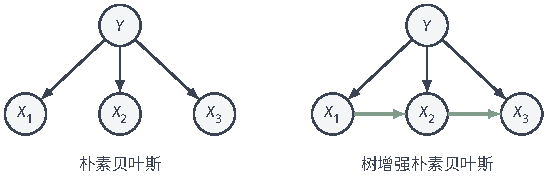
\includegraphics[width=92.650mm]{figures/06-probabilistic-graphical-models/04-models/tikz/pgm-static-directed-classifiers/figure.pdf}
  \caption{类别模型的两种属性结构。NB给定$Y$后各属性独立；TAN增加$X_1\to X_2\to X_3$，使右图的条件分布保留属性树上的依赖。训练时读入类别，预测时根据属性查询类别，观测状态随任务确定。}
  \label{fig:pgm-static-directed-classifiers}
\end{figure}

允许更大的父集，会增加需要估计的条件表。若属性$i$有$r_i$个状态，NB的自由参数为$(K-1)+K\sum_i(r_i-1)$；固定TAN属性树后，按父配置计数得到
\[
  (K-1)+K(r_r-1)
       +K\sum_{i\ne r}r_{t(i)}(r_i-1).
\]
两个类别和三个二值属性的自由参数由NB的$7$个增为TAN的$11$个，仍小于完整联合表所需参数，但新增父配置也需要数据支持。给定完整属性，两个模型枚举类别的评分均需$O(Kd)$次局部查询。二值TAN的对数评分还可含$x_i x_{t(i)}$项，因而能够表示属性间的交互。

TAN的学习包含参数估计与树选择两个层次。记定向后的属性树为$T$，固定它时，最大化
\begin{equation}
  \ell_T=\sum_{j=1}^n\left[
    \log\pi_{y_j}+\log p(x_{j,r}\mid y_j)
    +\sum_{i\ne r}\log p(x_{j,i}\mid y_j,x_{j,t(i)})\right].
  \label{eq:pgm-static-directed-tan-objective}
\end{equation}
每行条件表按类别与属性父值分组计数，再以该行总数归一化。树未知时，还需比较不同$T$各自达到的最大似然；下面把这个比较化成边权之和。选定树后重新按其父配置拟合条件表，便得到可用于类别预测的完整模型。

对于完整离散数据，可以选择使训练似然最大的属性树。先用经验分布$\widehat p$计算给定类别的条件互信息
\[
  \widehat I(X_i;X_j\mid Y)=
  \sum_{y,x_i,x_j}\widehat p(y,x_i,x_j)
  \log\frac{\widehat p(x_i,x_j\mid y)}
                 {\widehat p(x_i\mid y)\widehat p(x_j\mid y)}.
\]
求和只计算正频数项，零频数项以连续延拓取$0$。将候选树上的条件表分别拟合为最大似然表，其平均训练对数似然为
\begin{equation}
  \label{eq:pgm-static-directed-tan-score}
  -\widehat H(Y)-\sum_i\widehat H(X_i\mid Y)
  +\sum_{\{i,j\}\in E_{\mathrm{T}}}
       \widehat I(X_i;X_j\mid Y),
\end{equation}
这里$\widehat H$是经验熵，$E_{\mathrm T}$是属性树的无向边集。每个非根属性的条件熵可写为$H(X_i\mid Y,X_j)=H(X_i\mid Y)-I(X_i;X_j\mid Y)$，根仍贡献$H(X_r\mid Y)$；将各项相加，便得到式中的熵项与树边互信息。熵项不随树改变，因此以条件互信息为边权，求最大生成树并任取根定向即可。这个最大似然结论针对观测完整、无结构惩罚和自由条件表的设定，其他约束需重新分析得分。

若$r_i\le r$，直接统计全部属性对需$O(nd^2)$次计数更新，遍历条件表求边权需$O(Kd^2r^2)$操作，稠密最大生成树需$O(d^2)$时间。NB只统计单属性，计数为$O(nd)$。TAN增加这部分工作以拟合类内依赖，树结构仍限制可表达的高阶相互作用；数据稀疏时，新增条件表和不稳定的树边可能增加估计误差。Friedman等给出了TAN及其算法，结构学习的一般得分推导见第~\ref{chap:pgm-structure-learning}章\scite{pgm-static-directed-friedman1997}

\subsection{基于顺序条件的密度建模}
\label{sec:pgm-static-directed-autoregressive}

朴素贝叶斯需要一个已观测的类别节点来组织条件分布。若手头\emph{没有}类别标签、只想描述一条完整记录本身的联合分布，还有一个对任意联合分布都成立的通用办法：概率链式法则。它让我们人为给变量排一个顺序，然后把“整条记录的概率”写成第一个变量的边缘概率、给定第一个后第二个的条件概率、依此类推各项的连乘。这样做的好处是每一个因子都是一个归一化的条件分布，可以用功能很强的模型（如神经网络）逐个拟合，且无需引入任何潜变量、没有难以计算的积分；代价是要选定一个顺序，而且生成时只能沿该顺序逐个抽样。拟合观测的联合分布时，也可以依次为每个变量建立给定前面变量的条件分布。选定字段或像素的次序，把第$i$位以前的取值记为$\bm x_{<i}$。\term{自回归密度模型}（autoregressive density model）沿这个顺序计算条件概率，再相乘形成
\begin{equation}
  \label{eq:pgm-static-directed-ar}
  p_{\bm{\theta}}(\bm{x})
    =\prod_{i=1}^{d}p_{\bm{\theta}}(x_i\mid\bm{x}_{<i}).
\end{equation}
这种顺序规定预测前缀，例如表格字段排列或图像扫描顺序。第一个前缀$\bm x_{<1}$为空，因此第一项是边缘分布；各字段之间无需具有真实时间关系。

局部归一化保证式~\eqref{eq:pgm-static-directed-ar}的联合分布也归一化。离散变量先对$x_d$求和，最后一项变为$1$；依次消去$x_{d-1},\ldots,x_1$，最后留下$\sum_{x_1}p(x_1)=1$。连续变量使用非负可测、每个前缀下均归一化的条件密度，借助Tonelli定理依次积分，也得到总质量$1$。从某个联合分布恢复条件分布时，零概率前缀可补任意归一化条件分布，它与前缀零权重相乘后仍为零。归一化确定了概率合法性，拟合数据的质量还取决于所选条件函数。

链式法则允许任意联合分布沿任意变量排列分解。对二值变量使用完整条件表，仍需$1+2+\cdots+2^{d-1}=2^d-1$个自由参数。实际用有限宽度网络、有限感受野或高斯条件减少参数时，模型只保留这些局部函数可表达的分布。变量排列会改变待拟合的条件关系：一个方向的条件可能近似单峰，反向却可能出现多个峰，因此同样容量的函数在不同顺序下可产生不同误差。

消去例~\ref{ex:pgm-static-directed-binary}中的类别，得到两个读数的观测联合表
\[
  \begin{array}{ccccc}
    (x_1,x_2)&(0,0)&(0,1)&(1,0)&(1,1)\\
    p(x_1,x_2)&0.654&0.176&0.096&0.074
  \end{array}
\]
以$X_1$在前的顺序，将这张表改写为三个条件参数：
\[
  \begin{aligned}
    p(X_1=1)&=0.17,\\
    p(X_2=1\mid X_1=1)&=\frac{37}{85},\\
    p(X_2=1\mid X_1=0)&=\frac{88}{415}.
  \end{aligned}
\]
例如由$p(X_1=1)=0.17$和$p(X_2=1\mid X_1=1)=37/85$相乘，恢复$p(1,1)=0.074$。直接分解保留了整张读数联合表，用它能预测另一读数。若查询未观测工作状态$Y$，则还需要定义含$Y$的模型；观测表本身只给读数间的关系。

每个输出层需定义当前变量的完整条件分布。二值变量使用伯努利参数，有$r$个状态的变量使用softmax归一化概率；图像通道有$256$个离散值时，可以输出$256$项概率。连续条件可以输出均值$\mu_i(\bm x_{<i})$和正尺度$\sigma_i(\bm x_{<i})$来定义高斯密度，多峰条件则输出有限高斯混合的权重、均值和尺度。局部成分指示可被显式求和，因此混合参数化仍能计算这一条件似然。离散质量与连续密度使用不同的参考测度；将量化像素连续化时，还需给出量化区间积分或去量化方案。

完整训练记录提供每一位真实前缀，对这些条件分布的负对数似然求和，形成
\begin{equation}
  \label{eq:pgm-static-directed-ar-loss}
  L(\bm{\theta})=-\sum_{j=1}^{n}\sum_{i=1}^{d}
      \log p_{\bm{\theta}}
      (x_{j,i}\mid\bm{x}_{j,<i}).
\end{equation}
学习方法是把完整记录代入各条件函数，按式~\eqref{eq:pgm-static-directed-ar-loss}累加梯度，再更新共享参数。用小批量近似全数据梯度时，每个入选记录仍提供各位置的真实前缀。不同网络会采用逐步递推或同时前向计算，但共同优化的是这一个完整记录似然。额外的跨位置计算需要保持相同的读取约束，例如将全部输入汇总后广播到每个输出，会重新引入未来或当前目标信息。

生成记录时，条件所需的前缀尚待抽样。先取$X_1$，再据其结果取$X_2$，沿顺序继续，完成祖先采样。具有完整顺序依赖的标量模型要作$d$轮相继决策，不同记录可以批处理，同一记录则按前缀推进。缓存减少各轮重复计算，但前后状态的依赖仍保留。NB在类别给定后各属性独立，可并行抽样；TAN可按属性树的层次并行，生成顺序因此取决于具体父集。

自回归分解提供可计算的完整似然和顺序采样。观测的是前缀时，余下部分可按原条件分布续写；若第一位缺失、后面的多位已观测，计算第一位的后验可能需要汇总一批变量。选择模型时，应分别评估完整密度、祖先采样和任意条件补全的成本。第~\ref{chap:pgm-generative}章将沿用这条直接似然路线，与其他神经生成构造比较。

\subsubsection{NADE：复用逐步增长的前缀表示}
\label{sec:pgm-static-directed-nade-model}

用完整条件表实现自回归分解时，第$i$个条件分布要读取前面所有变量，参数表大小随$i$指数增长。换成神经网络拟合这些条件函数可以压缩参数量，但如果为每个位置$i$都各训练一个独立网络，又会有$d$个网络、彼此不共享，且无法利用“前$i$个变量的前缀”和“前$i+1$个变量的前缀”高度重叠这一事实。NADE的思路是让所有位置\emph{共用同一个网络}，并利用前缀只比上一步多一个变量的特点做增量计算：算出第$i$个条件所用的隐藏表示后，只需再加一项就能得到第$i+1$个条件的隐藏表示，而不必从头前向。逐前缀条件表的大小随维数增长。\term{神经自回归分布估计器}（neural autoregressive distribution estimator, NADE）让不同前缀共用网络参数，以限制需要保存的参数量。对二值观测，宽度为$h$的单隐藏层条件函数为
\begin{equation}
  \label{eq:pgm-static-directed-nade}
  \begin{aligned}
    \bm{a}_i&=\bm{c}+\sum_{j<i}\bm{W}_{:,j}x_j,&
    \bm{h}_i&=\operatorname{sigmoid}(\bm{a}_i),\\
    p(X_i=1\mid\bm{x}_{<i})
      &=\operatorname{sigmoid}
        (b_i+\bm{V}_{i,:}\bm{h}_i).
  \end{aligned}
\end{equation}
其中$\bm W\in\mathbb R^{h\times d}$、$\bm V\in\mathbb R^{d\times h}$，$\bm c,\bm b$为偏置，$\operatorname{sigmoid}(u)=(1+\exp(-u))^{-1}$。前缀从$i$延长到$i+1$时，用$\bm a_{i+1}=\bm a_i+\bm W_{:,i}x_i$增量更新，成本为$O(h)$；配合每位的输出计算，完整记录评价需$O(dh)$操作。$\bm h_i$由已知前缀确定，可直接计算，无需作为随机潜变量积分。这个前缀复用方式构成NADE计算似然的基础\scite{larochelle2011}

对式~\eqref{eq:pgm-static-directed-nade}输出的概率记$q_{j,i}$，NADE实际最小化的二值目标为
\[
 L_{\mathrm{NADE}}=-\sum_{j,i}
 [x_{j,i}\log q_{j,i}+(1-x_{j,i})\log(1-q_{j,i})].
\]
每轮沿前缀递推得到各$q_{j,i}$，将所有位置的误差信号反向传给共享的$\bm W,\bm V,\bm b,\bm c$，再作梯度更新。生成时把前一步抽得的值接入递推；有限隐藏宽度限制所能表示的条件函数，$O(dh)$计算量本身不保证拟合任意二值联合表。

\subsubsection{MADE：用掩码同时计算合法条件}
\label{sec:pgm-static-directed-made-model}

NADE要沿前缀一步步递推才能算完一条记录的似然，难以借助现代硬件一次性并行。于是产生一个诱人的想法：能不能让网络\emph{一次前向就同时输出}全部$d$个条件分布？难点在于自回归顺序要求“第$i$个输出只能看见前$i-1$个输入”，而普通全连接网络的每个输出能看见所有输入，会作弊地读到自己的当前值。MADE的解决办法非常直接：用一组固定的\emph{掩码}把违反顺序的连接权重强制置零，从结构上保证每个输出读取的恰好是它的合法前缀，从而在一次并行前向中算出全部条件。也可以同时计算各条件，但限制每个输出能读取的输入。\term{掩码自编码分布估计器}（masked autoencoder for distribution estimation, MADE）将违反自回归顺序的连接置零。给输入$j$次序号$j$、隐藏单元$u$次序号$m(u)$，仅保留输入边$j\le m(u)$与输出边$m(u)<i$。深层隐藏边的次序号非递减，输出端仍要求严格小于$i$，故每条输入到输出的路径都满足$j<i$。这样同时算出的第$i$个条件只使用合法前缀。

对单隐藏层二值输出，这些限制落实在权重矩阵上，模型结构可写成
\begin{equation}
  \bm h=\sigma((\bm W\odot\bm M_{\mathrm{in}})\bm x+\bm c),
  \qquad
  \bm q=\sigma((\bm V\odot\bm M_{\mathrm{out}})\bm h+\bm b),
  \label{eq:pgm-static-directed-made-structure}
\end{equation}
其中$\odot$为逐元素相乘，$\sigma$逐元素取sigmoid，$q_i$是第$i$个伯努利条件参数。训练使用与NADE相同的二值负对数似然，一次前向即可评价完整记录各位置；梯度只更新掩码允许的权重。生成时仍需先抽出第$i$位所依赖的前缀，再使用$q_i$，所以并行评价训练似然不等于并行生成整条记录。

图~\ref{fig:pgm-static-directed-mask}取三个输入和两个次序号分别为$1,2$的隐藏单元。以接收端为行、发送端为列，输入与输出掩码为
\[
  \bm{M}_{\mathrm{in}}=
  \begin{pmatrix}1&0&0\\1&1&0\end{pmatrix},\qquad
  \bm{M}_{\mathrm{out}}=
  \begin{pmatrix}0&0\\1&0\\1&1\end{pmatrix}.
\]
矩阵相乘得到$\left(\begin{smallmatrix}0&0&0\\1&0&0\\2&1&0\end{smallmatrix}\right)$，其非零项只在严格下三角，元素$2$计数两条合法路径。第一个条件输出仅用偏置，第三个输入只作为第三位似然的目标值，未进入任何条件参数。普通自编码器允许输出访问当前输入，可以通过复制完成重构。MADE结合前缀掩码与归一化条件输出，用各条件的负对数概率训练联合分布；这种似然目标需要由条件分布定义，普通重构误差则取决于另行选用的输出和损失\scite{pgm-static-directed-germain2015}

\begin{figure}[htbp]
  \centering
  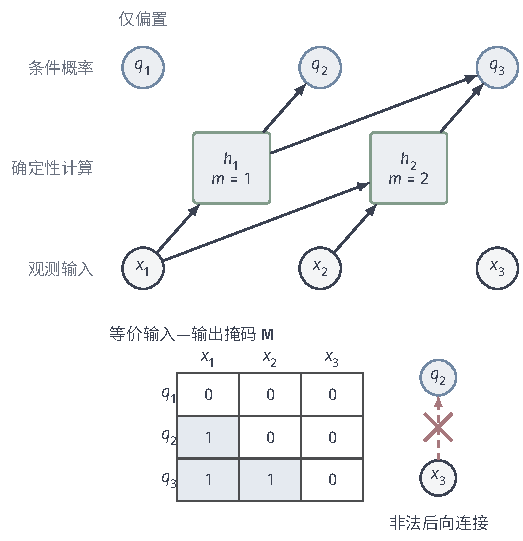
\includegraphics[width=88.554mm]{figures/06-probabilistic-graphical-models/04-models/tikz/pgm-static-directed-mask/figure.pdf}
  \caption{MADE掩码限定的条件依赖。隐藏方框进行确定性计算，输入与输出用圆框表示，$q_i=p(X_i=1\mid\bm x_{<i})$。下方输入—输出掩码中蓝色单元的1标出允许读取的前缀，右侧$x_3\to q_2$展示违反顺序的连接；各隐藏单元的次序号共同保证输出只能读取此前的输入。}
  \label{fig:pgm-static-directed-mask}
\end{figure}

\subsubsection{PixelCNN：把条件网络改为空间共享的掩码卷积}
\label{sec:pgm-static-directed-pixelcnn-model}

NADE、MADE都把输入当作一个没有空间结构的向量。但对图像而言，像素天然排布在二维网格上，同样的边缘、色块等局部图案会在图中不同位置反复出现；若为每个像素位置都单独保存一套连接权重，既浪费参数又无法利用这种“同一图案到处出现”的平移规律。卷积神经网络的优势正是让同一组卷积核在所有空间位置共享。于是只需把MADE的“掩码”思想搬到卷积上：按从上到下、从左到右的扫描顺序，让每个像素的条件网络只能读到它上方的行和同一行左侧的像素，就把空间权值共享与自回归的前缀约束结合起来。图像中相似的局部图案会出现在不同位置。为每个位置分别保存完整连接权重，没有利用这种重复；让相同卷积核在空间上复用，再屏蔽不合法的读取位置，就能把空间共享与前缀约束结合。

对图像，可用卷积共享不同位置的条件函数。\term{像素卷积自回归模型}（PixelCNN）按逐行扫描顺序，用掩码卷积读取当前像素上方和同行左侧的上下文。输入层排除当前目标值，后续层可读取当前位置已由合法前缀形成的隐藏表示。彩色图像还须规定像素内的通道顺序，例如红、绿、蓝，以使每个通道只访问此前通道。有限层数和卷积核限制可用感受野，模型虽归一化，却可能只利用部分前缀。原始论文同时介绍PixelCNN与PixelRNN，这里采用其中卷积掩码的依赖约束\scite{pgm-static-directed-oord2016}

具体到每通道$256$个离散值，网络在位置$i$输出得分$\bm f_{\bm\theta,i}$，条件结构与学习目标为
\begin{equation}
 \bm q_i=\operatorname{softmax}(\bm f_{\bm\theta,i}(\bm x_{<i})),
 \qquad L_{\mathrm{PixelCNN}}=-\sum_{j,i}\log q_{i,x_{j,i}}(\bm x_{j,<i}).
 \label{eq:pgm-static-directed-pixelcnn-objective}
\end{equation}
掩码卷积保证得分实际只读取允许的空间位置和此前通道，softmax保证各条件概率之和为$1$。每轮用真实图像前向计算所有条件，反向传播此目标并更新共享卷积核；生成则按同一像素和通道顺序抽样。NADE、MADE与PixelCNN因此共享自回归概率分解，改变的是前缀信息怎样计算、保存和复用。

\section{记录内共同变化的潜变量建模}
\label{sec:pgm-static-directed-latent}

聚类或压缩任务有时需要一个共同状态来解释多项读数。这个状态可以是每条记录选择的一种工作模式，也可以是连续变化的共同强度；本节先固定总体参数，研究一条记录内部的解释，跨记录的随机共享留到第~\ref{sec:pgm-static-directed-hierarchy-membership}节。为此可在观测外引入随机潜在坐标，再处理它们给定观测后的不确定性。\term{潜变量}（latent variable）指模型主动加入的未观测状态，漏记的字段则属于缺失数据，这一区别见第~\ref{sec:pgm-parameter-learning-definition}节。记潜在状态为$\bm z$，从它与观测的联合分布汇总得到
\begin{equation}
  \label{eq:pgm-static-directed-marginal}
  p_{\bm{\theta}}(\bm{x})=
  \begin{cases}
    \sum_{\bm{z}}p_{\bm{\theta}}(\bm{z})
          p_{\bm{\theta}}(\bm{x}\mid\bm{z}),
          &\text{离散潜变量},\\
    \int p_{\bm{\theta}}(\bm{z})
          p_{\bm{\theta}}(\bm{x}\mid\bm{z})\,d\bm{z},
          &\text{连续潜变量}.
  \end{cases}
\end{equation}
先验及各状态下的条件分布归一化，使观测分布的总质量为$1$。计算这个分布还要完成求和或积分，具体难度取决于潜变量和函数表示。仅由观测似然选择潜在解释时，也可能得到不同的等价分解；若要赋予它因果含义，需要更多依据。

\subsection{基于离散成分的混合建模}
\label{sec:pgm-static-directed-mixtures}

这一节转向本章的第二条主线：不再只在观测变量之间直接连边，而是为每条记录设想一个\emph{未观测的潜在状态}来解释它。先考虑最常见的情形——设备其实运行在若干离散的“工作模式”之一（如正常、过载、故障前兆），模式决定了这一整条记录的读数分布；但日志里并没有记录当前是哪种模式。把这个隐藏的模式选择记为$Z$，整条记录的分布就是“先按比例抽一种模式、再由该模式的分布生成读数”，对所有模式求和。这样一个“若干简单分布按比例混合”的模型就是有限混合模型；它同时解释了为什么单看两个读数会相关——它们只是共享了同一个隐藏模式。如果设备记录只含读数，工作状态可能由几个未标记的类别组成。\term{有限混合模型}（finite mixture model）先抽取成分，再用该成分的分布生成一条完整记录。成分$Z\in\{1,\ldots,K\}$具有权重$\pi_k\ge0$、$\sum_k\pi_k=1$，局部参数为$\bm\theta_k$，则
\begin{equation}
  \label{eq:pgm-static-directed-mixture}
  p(Z=k,\bm{x})=\pi_k p(\bm{x}\mid\bm{\theta}_k),
  \qquad
  p(\bm{x})=\sum_{k=1}^{K}\pi_kp(\bm{x}\mid\bm{\theta}_k).
\end{equation}
权重描述成分在总体中的比例，成分函数描述该状态下读数怎样变化。给定这些共享参数，每条记录独立抽取自己的$Z_j$，再生成观测。例~\ref{ex:pgm-static-directed-binary}若不记录类别，两个类内伯努利乘积就成为两成分混合；对类别求和后，仍得到前面的二元联合表。

有限混合的学习目标需要把没有记录的成分求和后再取对数：
\begin{equation}
 \max_{\bm\pi,\bm\theta_{1:K}}\;
 \ell_{\mathrm{mix}}=\sum_{j=1}^n\log\left[
    \sum_{k=1}^K\pi_kp(\bm x_j\mid\bm\theta_k)\right],
 \qquad \bm\pi\in\Delta^{K-1}.
 \label{eq:pgm-static-directed-mixture-objective}
\end{equation}
与NB的已知类别相比，每条记录现在不能直接归入一个计数组；其后验权重为$\pi_kp(\bm x_j\mid\bm\theta_k)/\sum_\ell\pi_\ell p(\bm x_j\mid\bm\theta_\ell)$。这些权重随参数变化，所以目标中的成分不再能像已标注类别那样分别优化。以下先说明混合解释相关性的机制，再用高斯成分展开EM。

共同成分怎样产生读数相关，可以把协方差分成类内和类间两部分。对具有有限二阶矩的两个属性，全协方差公式给出
\[
  \operatorname{Cov}(X_1,X_2)=
  \mathbb{E}\!\left[\operatorname{Cov}(X_1,X_2\mid Z)\right]
  +\operatorname{Cov}\!\left(
       \mathbb{E}[X_1\mid Z],\mathbb{E}[X_2\mid Z]\right).
\]
成分内部条件独立时，第一项为零，类间均值的共同变化仍可使第二项非零。前面二值读数的类间项为$0.1\times0.9\times(0.8-0.1)\times(0.7-0.2)=0.0315$，与联合表一致。若成分内部还有相关性，则保留第一项；有限混合本身并不规定成分内属性独立。

当读数是连续值时，最常用的成分分布是高斯分布；单个高斯只有一个峰、呈椭球状，无法描述“数据聚成好几团、每团中心和形状都不同”的情形，而把若干个高斯按比例混合，就能拼出多峰、任意形状的复杂分布。连续读数可以采用\term{高斯混合模型}（Gaussian mixture model, GMM）：$p(\bm x\mid Z=k)=\mathcal N(\bm x;\bm\mu_k,\bm\Sigma_k)$，各协方差正定。全协方差以$d(d+1)/2$个参数允许不同方向的相关和伸展；对角协方差以$d$个参数表示条件独立的属性；球形$\sigma_k^2\bm I$只估一个尺度。也可要求所有成分共享协方差，减少参数并让各成分具有同样形状。每个成分即使使用对角协方差，混合后的类间变化仍能形成非对角的总体协方差。

GMM将高斯成分代入式~\eqref{eq:pgm-static-directed-mixture-objective}，具体模型与目标是
\begin{equation}
 p(\bm x)=\sum_k\pi_k\mathcal N(\bm x;\bm\mu_k,\bm\Sigma_k),
 \qquad
 \ell_{\mathrm{GMM}}=\sum_j\log\sum_k\pi_k
          \mathcal N(\bm x_j;\bm\mu_k,\bm\Sigma_k).
 \label{eq:pgm-static-directed-gmm-objective}
\end{equation}
优化变量为权重、均值和满足选定约束的正定协方差；固定成分数$K$时，这才是EM要提高的观测目标。

固定参数后，用每个成分的先验权重乘该记录的密度，再对$K$项归一化，就得到\term{责任度}（responsibility），即记录属于各成分的后验概率。对高斯成分，第$t$轮参数下写成
\begin{equation}
  \label{eq:pgm-static-directed-responsibility}
  r_{j,k}^{(t)}=
  \frac{\pi_k^{(t)}
      \mathcal{N}(\bm{x}_j;\bm{\mu}_k^{(t)},\bm{\Sigma}_k^{(t)})}
       {\sum_{\ell=1}^{K}\pi_\ell^{(t)}
      \mathcal{N}(\bm{x}_j;\bm{\mu}_\ell^{(t)},\bm{\Sigma}_\ell^{(t)})}.
\end{equation}
对前面的二值混合，观测$(1,1)$属于异常成分的责任度同样是$28/37$。将类别作为潜在成分时，这些后验权重需要由当前参数推断，参数又要依据这些记录的归属来估计，两项计算因而交替进行。

EM在每轮先用旧参数计算式~\eqref{eq:pgm-static-directed-responsibility}中的责任度，再固定这些权重，优化新参数，通用推导见第~\ref{chap:pgm-parameter-learning}章。对高斯混合，需要最大化的期望完全数据对数似然为
\[
  \begin{aligned}
    Q={}&\sum_{j,k}r_{j,k}^{(t)}
       \left(\log\pi_k-\frac12\log|\bm{\Sigma}_k|\right)\\
       &-\frac12\sum_{j,k}r_{j,k}^{(t)}
         (\bm{x}_j-\bm{\mu}_k)^\top
          \bm{\Sigma}_k^{-1}(\bm{x}_j-\bm{\mu}_k)
       +\text{常数}.
  \end{aligned}
\]
在$\sum_k\pi_k=1$下对权重求驻点，得到加权样本比例；均值驻点为加权观测均值；将它代入协方差项，得到加权残差二阶矩。记有效样本数$N_k^{(t)}=\sum_jr_{j,k}^{(t)}$，当它为正且协方差更新保持正定时，三个更新为
\begin{equation}
  \label{eq:pgm-static-directed-gmm-em}
  \begin{aligned}
    \pi_k^{(t+1)}&=\frac{N_k^{(t)}}{n},\\
    \bm{\mu}_k^{(t+1)}
      &=\frac{\sum_jr_{j,k}^{(t)}\bm{x}_j}{N_k^{(t)}},\\
    \bm{\Sigma}_k^{(t+1)}
      &=\frac{1}{N_k^{(t)}}\sum_jr_{j,k}^{(t)}
       (\bm{x}_j-\bm{\mu}_k^{(t+1)})
       (\bm{x}_j-\bm{\mu}_k^{(t+1)})^\top.
  \end{aligned}
\end{equation}
协方差约束决定最后一步怎样汇总残差：对角模型取对角元素，球形模型取迹再除以$d$。这两种更新直接极大化各自的受约束目标，估计过程中始终使用相应的协方差形式。

\begin{example}[一轮可复核的高斯混合EM]
  \label{ex:pgm-static-directed-gmm-em}
  取一维人工记录$x_1=-1,x_2=1$，两个成分初始权重均为$1/2$、均值为$-1,1$、方差均为$1$。在$x_1$处，两成分的加权密度比为$1:\exp(-2)$，责任度矩阵为
  \[
    \bm{R}^{(0)}
      =\begin{pmatrix}a&1-a\\1-a&a\end{pmatrix},
    \qquad a=\frac{1}{1+\exp(-2)}\approx0.880797.
  \]
  两个成分的有效样本数各为$1$，所以新权重均仍为$1/2$；均值更新得到$\mu_1^{(1)}=1-2a\approx-0.761594$、$\mu_2^{(1)}=2a-1$。样本平方均为$1$，加权二阶矩也为$1$，减去新均值的平方得到
  \[
    (\sigma_1^2)^{(1)}=(\sigma_2^2)^{(1)}
      =1-(2a-1)^2\approx0.419974.
  \]
  责任度同时为两个成分保留正权重，两个新均值因此向中间移动；方差再围绕这些新均值估计。例子展示一次E步与M步的数值变化，尚未评价多轮优化的终点或新数据上的表现。
\end{example}

全协方差GMM先分解$K$个协方差矩阵，成本为$O(Kd^3)$，再计算$nK$个二次型及加权协方差统计，通常需$O(nKd^2)$操作。对角表示将统计成本降为$O(nKd)$。固定参数时，有限混合的似然与成分后验由可计算的$K$项得到，精确求和保持可行；学习还需求解非凸优化并选择成分数。计算责任度时可先求对数权重，减去最大值，再指数化归一化，以降低高维密度下溢的风险。

含至少两个成分、协方差无正下界的GMM存在以下退化路径：把某成分均值放到一个训练点，将协方差趋于零，该点的密度趋于无穷；其余成分继续覆盖其他记录，训练似然便可没有有限最大值。继续迭代少量样本的例子也会面临这种边界。协方差特征值下界、适当先验或受约束估计可限制这类路径，但相应地改变学习目标；手工重置成分还需另行检查单调性。实际可从分散记录或聚类中心多次初始化，比较所得解；有效样本数近零时，按预定规则处理空成分。选择成分数时，再结合留出似然和应用任务，评估新增成分在训练数据以外的收益。

参数还具有\term{标签交换}（label switching）对称性。对任意两个成分，同时交换权重、均值和协方差，式~\eqref{eq:pgm-static-directed-mixture}给出的观测分布完全相同，编号本身无法由数据确定。置换得到的是同一预测分布的命名变化，另一个局部极值则可能给出不同预测。某些混合族在条件满足时可除置换外识别，但这个两成分、两二值属性例子有$5$个自由参数，观测表仅有$3$个自由度，通常还存在其他非唯一分解。解释成分或汇总对称后验时，应保留这种差异：不同编号的参数直接平均，可能破坏原本有用的预测表示。Murphy的教材讨论混合分布及其估计\scite{pgm-murphy2012}

\subsection{基于连续因子的观测建模}
\label{sec:pgm-static-directed-linear-gaussian}

离散混合假设每条记录\emph{恰好属于}一个隐藏类别，是“非此即彼”的归属。但很多共同原因本身是连续变化的：负载、振动强度、环境温度都可强可弱，一条记录往往同时受到\emph{好几个}强弱不同的共同因素影响，而不是只选其中一个。这时更自然的模型是用几个连续的潜在“因子”线性叠加来解释观测，剩下解释不了的部分归于每个传感器独有的噪声；这就是因子分析。它把每个观测读数理解成“少数共同因子的加权组合＋自身噪声”，从而用降维后的连续坐标刻画记录之间的共同变化。离散混合让一条记录选择一种模式；连续因子模型则允许同一条记录同时带有多个强弱不同的共同因素。两者都通过潜变量解释观测关系，但潜在状态的含义、汇总运算和后验形式不同。

\subsubsection{因子分析：把相关性分成共同因子与独有噪声}
\label{sec:pgm-static-directed-fa-model}

多个读数也可能随连续的负载或振动强度共同变化。用$q<d$个潜在坐标表示这部分变化，剩余各维由独有噪声解释，就得到\term{因子分析}（factor analysis, FA）的线性高斯模型
\begin{equation}
  \label{eq:pgm-static-directed-fa}
  \begin{aligned}
    \bm{Z}&\sim\mathcal{N}(\bm{0},\bm{I}_q),\\
    \bm{X}&=\bm{\mu}+\bm{W}\bm{Z}+\bm{\varepsilon},\\
    \bm{\varepsilon}&\sim\mathcal{N}(\bm{0},\bm{\Psi}),\qquad
    \bm{\Psi}=\operatorname{diag}(\psi_1,\ldots,\psi_d),
    \quad\psi_i>0.
  \end{aligned}
\end{equation}
潜变量$\bm Z$与噪声$\bm\varepsilon$独立，$\bm\mu\in\mathbb R^d$是观测均值，载荷$\bm W\in\mathbb R^{d\times q}$的每列说明一个潜在坐标怎样同时影响各读数。给定所有潜在坐标，均值中的各因子贡献相加，观测只剩对角协方差的独立噪声。

线性变换保留高斯形式，独立的潜在贡献与噪声又使协方差相加，因此积分消去潜变量后得到
\begin{equation}
  \label{eq:pgm-static-directed-fa-marginal}
  \bm{X}\sim\mathcal{N}(\bm{\mu},\bm{C}),\qquad
  \bm{C}=\bm{W}\bm{W}^{\top}+\bm{\Psi}.
\end{equation}
共同变化$\bm W\bm W^\top$的秩至多为$q$，对角$\bm\Psi$记录各传感器独有的噪声。这个约束规定了相关性必须由共同因子解释。若让噪声协方差完全自由，噪声也能吸收观测相关，因子与噪声间的分配就更加不确定。

模型结构确定后，学习希望让这些高斯边缘分布解释完整训练记录。令$\bm C=\bm W\bm W^\top+\bm\Psi$，FA的观测目标为
\begin{equation}
 \ell_{\mathrm{FA}}(\bm\mu,\bm W,\bm\Psi)
   =\sum_j\log\mathcal N(\bm x_j;\bm\mu,\bm C),
 \qquad \bm\Psi\text{为正对角矩阵}.
 \label{eq:pgm-static-directed-fa-objective}
\end{equation}
对固定正定$\bm C$，对均值求导得到$\widehat{\bm\mu}=\overline{\bm x}$。将均值固定为这个样本均值，记$\bm y_j=\bm x_j-\overline{\bm x}$、$\bm S_x=n^{-1}\sum_j\bm y_j\bm y_j^\top$，去掉与$\bm W,\bm\Psi$无关的常数后，等价于最小化
\[
 \frac n2\left[\log|\bm C|+
                  \operatorname{tr}(\bm C^{-1}\bm S_x)\right].
\]
第一项惩罚无界扩张协方差，第二项评价观测偏差相对于模型协方差的大小；二者共同决定拟合，不能只压低残差。直接优化这个目标是一条路线，EM则先计算每条记录潜在因子的后验矩，再用这些矩更新载荷和噪声。

给定观测，需要估计潜在坐标及其误差。令中心化读数$\bm y=\bm x-\bm\mu$，后验二次项系数$\bm M=\bm I_q+\bm W^\top\bm\Psi^{-1}\bm W$，先验与条件密度相乘后的$\bm z$项为
\[
  \begin{aligned}
    -2\log p(\bm{z}\mid\bm{x})
      &=\bm{z}^{\top}\bm{z}
       +(\bm{y}-\bm{W}\bm{z})^{\top}
          \bm{\Psi}^{-1}(\bm{y}-\bm{W}\bm{z})
       +\text{常数}\\
      &=\bm{z}^{\top}\bm{M}\bm{z}
       -2\bm{z}^{\top}\bm{W}^{\top}\bm{\Psi}^{-1}\bm{y}
       +\text{常数}.
  \end{aligned}
\]
正定噪声使$\bm M$正定。对上式配方，写成$(\bm z-\bm m)^\top\bm M(\bm z-\bm m)+\text{常数}$，读取高斯中心和精度，得到
\begin{equation}
  \label{eq:pgm-static-directed-fa-posterior}
  \begin{aligned}
    p(\bm{z}\mid\bm{x})&=\mathcal{N}(\bm{z};\bm{m},\bm{S}),\\
    \bm{S}&=\bm{M}^{-1},\qquad
    \bm{m}=\bm{S}\bm{W}^{\top}\bm{\Psi}^{-1}
                  (\bm{x}-\bm{\mu}).
  \end{aligned}
\end{equation}
后验均值表示给定读数的潜在坐标估计，后验协方差量化剩余不确定性。权重$\bm\Psi^{-1}$让噪声较小的测量在相同载荷下贡献较多精度，先验则提供单位精度，使证据较弱的坐标向零收缩。在固定参数、完整观测的条件下，协方差由$\bm M$决定，读数数值只改变后验均值。

对独立同分布的完整记录，已将FA的均值固定为样本均值，以下以$\bm y_j=\bm x_j-\overline{\bm x}$中心化。E步用旧参数和式~\eqref{eq:pgm-static-directed-fa-posterior}得到$\bm m_j,\bm S$，并形成二阶矩$\bm T_j=\bm S+\bm m_j\bm m_j^\top=\mathbb E[\bm Z_j\bm Z_j^\top\mid\bm x_j]$。M步对期望加权残差目标中的载荷求导，得到
\[
  \bm{W}^{(t+1)}\sum_j\bm{T}_j
     =\sum_j\bm{y}_j\bm{m}_j^\top.
\]
这个矩阵方程右乘$\left(\sum_j\bm T_j\right)^{-1}$，可写出载荷更新。每项$\bm T_j$都包含正定$\bm S$，所以在正噪声与有限参数的当前迭代下，系数矩阵可逆。实际计算可直接求解矩阵方程，避免显式构造逆矩阵。

估计噪声时，还需把潜在坐标的后验方差计入残差。用$\bm W_+=\bm W^{(t+1)}$表示新载荷，期望残差协方差为
\begin{equation}
  \label{eq:pgm-static-directed-fa-residual}
  \begin{aligned}
    \bm{R}=\frac1n\sum_j\bigl[
      &(\bm{y}_j-\bm{W}_{+}\bm{m}_j)
       (\bm{y}_j-\bm{W}_{+}\bm{m}_j)^\top\\
      &+\bm{W}_{+}\bm{S}\bm{W}_{+}^\top
    \bigr].
  \end{aligned}
\end{equation}
FA逐维取$\psi_i^{(t+1)}=\bm R_{i,i}$。残差的第二项将潜变量后验方差映射到观测空间；若省掉它，就少计了一项半正定协方差贡献，噪声估计可能偏小。解析E步和这项M步共同构成模型的EM迭代，单调性条件见第~\ref{chap:pgm-parameter-learning}章。噪声趋于零时，还需检查边界解和数值条件。

\subsubsection{概率主成分分析及线性因子模型的查询}
\label{sec:pgm-static-directed-ppca-model}

将残余噪声约束为$\bm\Psi=\sigma^2\bm I_d$，得到\term{概率主成分分析}（probabilistic principal component analysis, PPCA）。FA分别估计每维噪声，PPCA要求在当前坐标单位下各方向噪声同方差。改变特征单位会改变后一假设的含义，因此尺度选择需要与噪声模型一致。两种模型都提供潜在表示，同时给出这些坐标的后验不确定性。

PPCA沿用式~\eqref{eq:pgm-static-directed-fa-objective}，但把候选协方差限制为$\bm C=\bm W\bm W^\top+\sigma^2\bm I_d$、$\sigma^2>0$。它仍估计样本均值，在同一协方差目标下只优化$\bm W$和共同噪声方差。EM的E步及载荷更新不变，只需在相应矩阵中代入各向同性噪声；噪声M步变为$(\sigma^2)^{(t+1)}=\operatorname{tr}(\bm R)/d$。这一步把各维期望残差平均，正是共同方差约束下的极大化结果。

PPCA的最大似然载荷也可由样本协方差求得。令$\bm S_x=n^{-1}\sum_j\bm y_j\bm y_j^\top$，特征值按$\lambda_1\ge\cdots\ge\lambda_d$排列，前$q$个特征向量组成$\bm U_q$。当其余特征值的平均值为正时，解为
\begin{equation}
  \label{eq:pgm-static-directed-ppca-ml}
  \begin{aligned}
    \widehat{\sigma}^2
      &=\frac{1}{d-q}\sum_{i=q+1}^{d}\lambda_i,\\
    \widehat{\bm{W}}
      &=\bm{U}_q
       (\bm{\Lambda}_q-\widehat{\sigma}^2\bm{I}_q)^{1/2}
       \bm{R}_0,\qquad
       \bm{R}_0\bm{R}_0^\top=\bm{I}_q,
  \end{aligned}
\end{equation}
其中$\bm\Lambda_q=\operatorname{diag}(\lambda_1,\ldots,\lambda_q)$。负对数似然的协方差项为$\log|\bm C|+\operatorname{tr}(\bm C^{-1}\bm S_x)$：固定模型特征值，迹的重排不等式要求把最大的模型方差与最大的观测方差对齐。此后每个自由方向贡献$\log c_i+\lambda_i/c_i$，在$c_i=\lambda_i$处最小；其余$d-q$维共用$\sigma^2$，对这部分总和求导就得到剩余特征值的平均数。保留方向的重根会产生主轴选择的不唯一性；噪声估计为零则到达奇异边界，正定高斯密度的公式需重新处理。Tipping与Bishop给出了这个似然解及EM方法\scite{tipping1999}

为比较概率表示与几何投影，在保留的$\lambda_i>\widehat\sigma^2$方向，将潜变量后验均值映回观测空间，得到
\[
  \widehat{\bm{W}}\bm{m}
    =\bm{U}_q\operatorname{diag}
       \left(1-\frac{\widehat{\sigma}^2}{\lambda_i}\right)_{i=1}^{q}
       \bm{U}_q^\top\bm{y}.
\]
PCA把读数正交投影到所选子空间，PPCA还按信噪比缩小其中的坐标。固定满列秩载荷并令$\sigma^2$趋于零，均值重构的极限才是列空间上的正交投影；零噪声处的模型分布位于低维支持，已不是全维正密度。这样可由有噪声的后验重构联系降维几何，同时保留噪声条件的作用。

取人工样本协方差的特征值$5,2,1$，只保留一个因子。PPCA估计$\widehat\sigma^2=(2+1)/2=1.5$，可选$\widehat{\bm W}=\sqrt{3.5}\bm u_1$，得到模型协方差特征值$5,1.5,1.5$。后两方向被共同噪声方差合并，潜变量后验方差为$(1+3.5/1.5)^{-1}=0.3$。均值重构为$0.7\bm u_1\bm u_1^\top\bm y$，显示相对于PCA投影的收缩幅度。

某些传感器未读取时，潜在状态的不确定性随证据减少而变化。记观测索引$O\subseteq\{1,\ldots,d\}$，缺失索引为$U$，在式~\eqref{eq:pgm-static-directed-fa-posterior}中只保留$\bm W_{O,:}$、$\bm\Psi_{O,O}$及$\bm x_O-\bm\mu_O$，得到$\bm m_O,\bm S_O$。再利用独立残余噪声，把这些后验矩传播到缺失读数，得到
\begin{equation}
  \label{eq:pgm-static-directed-fa-missing}
  \begin{aligned}
    \mathbb{E}[\bm{X}_U\mid\bm{x}_O]
      &=\bm{\mu}_U+\bm{W}_{U,:}\bm{m}_O,\\
    \operatorname{Cov}(\bm{X}_U\mid\bm{x}_O)
      &=\bm{\Psi}_{U,U}
        +\bm{W}_{U,:}\bm{S}_O\bm{W}_{U,:}^\top.
  \end{aligned}
\end{equation}
缺失读数的预测方差包括自身噪声$\bm\Psi_{U,U}$，以及共同因子尚不确定带来的$\bm W_{U,:}\bm S_O\bm W_{U,:}^\top$。填入条件均值只保存一个估计值；后续使用填补数据时，还需处理这两项预测误差。

\begin{example}[两台传感器对一个连续因子的测量]
  \label{ex:pgm-static-directed-fa-missing}
  取$q=1,d=2$、$\bm\mu=\bm{0}$、$\bm W=(1,2)^\top$和$\bm\Psi=\operatorname{diag}(1,4)$作为人工模型，观测协方差为
  \[
    \bm{C}=\begin{pmatrix}2&2\\2&8\end{pmatrix}.
  \]
  完整读数$(2,4)$给出后验精度$1+1^2/1+2^2/4=3$、线性项$1\times2/1+2\times4/4=4$，所以$Z\mid(2,4)\sim\mathcal N(4/3,1/3)$。

  只保留$X_1=2$，后验精度变为$2$，得到$Z\mid X_1=2\sim\mathcal N(1,1/2)$。第二读数的预测均值为$2\times1=2$，方差为$4+2^2/2=6$。在观测空间直接条件化，也得到均值$(2/2)\times2=2$和方差$8-2^2/2=6$，两条计算路线一致。
\end{example}

载荷及坐标存在\term{旋转不唯一性}（rotational non-identifiability）。任意正交$\bm R_0$下，将载荷变为$\bm W\bm R_0$、坐标变为$\bm R_0^\top\bm Z$，潜在先验和观测协方差都保持原样。数据似然因而只约束相应分布，一维时也无法确定因子符号。为把某个因子命名为物理强度，需要额外约束、实验或领域信息；FA还可能有载荷和独有噪声的其他分解歧义。

对完整记录和对角噪声，形成$\bm M$需$O(dq^2)$操作，分解它需$O(q^3)$；复用相关矩阵后，各记录后验均值的计算为$O(dq)$。用Woodbury恒等式和行列式引理，也能以潜在空间矩阵计算观测似然：
\[
  \bm{C}^{-1}=\bm{\Psi}^{-1}
    -\bm{\Psi}^{-1}\bm{W}\bm{S}\bm{W}^{\top}\bm{\Psi}^{-1},
  \qquad |\bm{C}|=|\bm{\Psi}|\,|\bm{M}|,
\]
这两个恒等式使密度评价可避开$d\times d$稠密分解。完整数据的一轮EM通常为$O(ndq+nq^2+dq^2+q^3)$，噪声更新只计算残差协方差的对角元素。相同缺失模式可共用后验精度，不同模式需分别形成矩阵。缺失数据的E步还要计算缺失量的条件矩，均值更新也要利用这些矩。只对已观测数据最大化似然的适用条件，需结合第~\ref{chap:pgm-parameter-learning}章的缺失机制与可忽略性分析。

\section{跨记录与分组观测的共享建模}
\label{sec:pgm-static-directed-hierarchy-membership}

前两节的模型都把$n$条记录看作来自同一个总体、彼此独立同分布。但现实数据常常是\emph{分组}的：记录来自不同工厂、不同用户、不同文档。同型号设备在不同工厂工作，各厂参数可能相似又各有偏差；同一文档也可能同时包含设备和维修等多个主题。这类任务需要进一步规定哪些未知量跨记录共享、哪些选择在记录内部变化。本节分别考察组参数来自共同总体、组内逐项使用共享成分，以及随机成分库怎样跨记录或跨组复用。这些机制可组合；共享一个固定参数并不等于已经为组间异质性建立了随机层次。

\subsection{组参数的共享与部分汇聚}
\label{sec:pgm-static-directed-partial-pooling}

设有的工厂仅提供两条测量，另一些工厂提供几十条。各厂独立估计能够保留差异，却使小样本厂的均值波动很大；完全合并则要求所有工厂共用均值。让每厂有自己的均值，同时把这些均值放进一个共同总体，便在两种极端之间留下可估计的共享程度。

在“每组各估一套参数”和“所有组合并成一套参数”这两个极端之间，存在一个自然的折中：让每组拥有自己的参数，但规定这些组参数都\emph{抽自同一个共享的上层分布}。于是数据多的组主要由自己的数据决定，数据少的组则被向上层中心“拉一把”，各组还能通过这个共同上层互相借力。\term{层次模型}（hierarchical model）让各组参数来自一个共享的上层分布，以联系组间规律。\term{板表示法}（plate notation）用带索引的框标出节点与边的重复范围：组板内、样本板外的节点每组复制一次，两板内部的节点在每组的每个样本复制一次。给定索引后展开这些副本及连接，就得到联合分解的完整图。板框表示重复组织，概率因子仍由展开后的节点和父集决定。

例如组$g$的测量服从$X_{g,j}\mid\mu_g\sim\mathcal N(\mu_g,\sigma^2)$，组均值来自$\mu_g\sim\mathcal N(m_0,\tau^2)$。给定组均值，所有测量独立；给定上层参数，各组均值也独立。取已知$m_0$及正数$\sigma^2,\tau^2$，组内$n_g$条记录的均值为$\overline x_g$，配方得到
\begin{equation}
  \label{eq:pgm-static-directed-pooling}
  \begin{aligned}
    \mathbb{E}[\mu_g\mid\bm{x}_g]
      &=a_g\overline x_g+(1-a_g)m_0,\\
    a_g&=\frac{n_g\tau^2}{\sigma^2+n_g\tau^2},\\
    \operatorname{Var}(\mu_g\mid\bm{x}_g)
      &=\left(\tau^{-2}+n_g\sigma^{-2}\right)^{-1}.
  \end{aligned}
\end{equation}
权重$a_g$随组内样本数增加而增大，随测量噪声增加而减小，后验均值在本组平均值与共享中心$m_0$之间变化。这正是\term{部分汇聚}（partial pooling）的含义：既不像“完全不汇聚”那样让小样本组各自为战、估计剧烈波动，也不像“完全汇聚”那样强行抹平所有组的差异，而是在保留组间差异的同时，用共同分布把数据较少的组向中心收缩，收缩多少由该组数据量自动决定。取人工参数$m_0=0,\tau^2=1,\sigma^2=4,\overline x_g=3$，两条测量得到后验均值$1$，二十条测量得到$2.5$。两种收缩程度来自先验与测量精度的相对比例。

这一组层与样本层结构也直接给出观测分布。令$\bm x_g$收集工厂$g$的$n_g$条记录，$\bm1$为$n_g$维全1向量，积分掉$\mu_g$得到
\[
 \bm X_g\sim\mathcal N(m_0\bm1,
       \sigma^2\bm I_{n_g}+\tau^2\bm1\bm1^\top).
\]
组内不同记录因共同均值而具有协方差$\tau^2$。固定超参数时，各组之间仍独立，这与把全组数据当作独立测量的似然不同。

若共享参数需要从数据估计，经验贝叶斯的明确目标是
\begin{equation}
 \ell_{\mathrm{EB}}(m_0,\tau^2,\sigma^2)
 =\sum_g\log\int\mathcal N(\mu_g;m_0,\tau^2)
                \prod_j\mathcal N(x_{g,j};\mu_g,\sigma^2)\,d\mu_g.
 \label{eq:pgm-static-directed-pooling-objective}
\end{equation}
这里优化$m_0$及待估的正方差；若$\sigma^2$已知，就固定它。EM用旧超参数和式~\eqref{eq:pgm-static-directed-pooling}得到组后验均值$m_g$与方差$s_g^2$，再更新
\[
 \begin{aligned}
 m_0^+&=G^{-1}\sum_gm_g, &
 (\tau^2)^+&=G^{-1}\sum_g[(m_g-m_0^+)^2+s_g^2],\\
 (\sigma^2)^+&=\frac{\sum_{g,j}[(x_{g,j}-m_g)^2+s_g^2]}{\sum_g n_g}.
 \end{aligned}
\]
$G$是组数，加号表示本轮的新参数；每个方差更新同时包括均值残差和后验不确定性。重新计算组后验后继续迭代，检查边缘似然变化、方差边界和停止容差，不能用一次组均值平均替代整个学习过程。

式~\eqref{eq:pgm-static-directed-pooling}中的共享分布固定已知时，本组后验只读取本组数据；其他组的新增记录不会改变它。若用全部组估计$m_0,\tau^2$，或为它们设先验再联合推断，各组便通过未知共享量交换信息。例如将$\mu_g$作为潜在组参数进行EM，E步求其后验矩，共同$\tau^2$下的M步将$m_0$更新为各组$\mathbb E[\mu_g\mid\mathcal D]$的平均。完全贝叶斯方法继续积分共享参数的不确定性。组级分布假设需要与组间规律相符，否则向同一中心收缩会引入偏差。

完全贝叶斯分析为$\bm h=(m_0,\tau^2,\sigma^2)$指定适当先验，目标变为
\[
 p(\bm h,\mu_{1:G}\mid\mathcal D)
 \propto p(\bm h)\prod_g p(\mu_g\mid\bm h)
                         \prod_jp(x_{g,j}\mid\mu_g,\bm h).
\]
可以交替更新组均值与共享参数的条件后验，不能解析的部分使用前文的采样或变分计算。固定超参数时，已有组下一条记录的预测为$\mathcal N(m_g,\sigma^2+s_g^2)$；尚无数据的新组则为$\mathcal N(m_0,\sigma^2+\tau^2)$。完全贝叶斯预测还要对$\bm h$的后验积分，经验贝叶斯则把拟合的$\bm h$直接代入，两种输出对共享参数不确定性的处理不同。

\subsection{组内逐项分配与混合成员}
\label{sec:pgm-static-directed-mixed-membership}

有限混合模型给\emph{整条记录}只分配一个隐藏类别——一台设备要么正常、要么异常，一篇文档要么属于这个主题、要么属于那个主题。但很多对象天然是“多种成分按比例混合”的：一篇文档往往同时讨论设备、维修、安全等多个主题，不同段落甚至不同词语各自侧重不同主题。于是更细的做法是把分配单位从“整条记录”下沉到“记录里的每一项”：整组持有一个关于各成分的\emph{比例}，组内每个观测再按这个比例各自挑选成分。同一组中每个局部观测还可以选择自己的成分，这种结构称为\term{混合成员}（mixed membership）。一篇同时讨论设备和维修的文档，每个词分别选择主题，文档的主题比例控制这些选择；主题本身是词概率分布，其语义名称需由数据和应用解释。设文档$g=1,\ldots,G$有$N_g$个词，词表大小为$v$，词编号为$X_{g,j}\in\{1,\ldots,v\}$。主题词概率向量$\bm\beta_k$与文档主题比例$\bm\pi_g$各自非负、分量和为$1$。

\subsubsection{pLSA：每篇文档拥有固定比例，每个词选择主题}
\label{sec:pgm-static-directed-plsa-model}

先看混合成员思想最朴素的实现：不给文档主题比例的来源建模，而是把每篇训练文档的比例直接当作一组需要估计的\emph{自由参数}。有限混合为整条记录只抽一个成分，不能直接描述一篇文档在不同词位置使用不同主题的过程。让文档持有一组比例、每个词重新选择主题，就能保留文档内的多主题构成。

\term{概率潜在语义分析}（probabilistic latent semantic analysis, pLSA）为每篇训练文档估计一个固定比例$\bm\pi_g$。给定文档编号，词位置$j$先从$\operatorname{Categorical}(\bm\pi_g)$抽主题$Z_{g,j}$，再从相应$\bm\beta_{Z_{g,j}}$抽词，得到
\begin{equation}
  \label{eq:pgm-static-directed-plsa}
  p(\bm{x}_g\mid\bm{\pi}_g,\bm{\beta}_{1:K})
    =\prod_{j=1}^{N_g}
       \sum_{k=1}^{K}\pi_{g,k}\beta_{k,x_{g,j}}.
\end{equation}
$\operatorname{Categorical}$给出类别抽样概率，$\beta_{k,a}$是主题$k$产生词$a$的概率。给定固定比例与主题参数，不同词各有自己的主题后验，权重正比于$\pi_{g,k}\beta_{k,x_{g,j}}$，各位置的后验独立。EM用这些责任度更新文档比例为平均主题责任度，再按全语料加权词频更新主题分布。相同词可合并为词频以复用计算。Hofmann介绍了pLSA的混合分解与EM估计\scite{pgm-static-directed-hofmann1999}

pLSA的目标与学习步骤可以写成一组可执行的更新。最大化
\begin{equation}
 \ell_{\mathrm{pLSA}}=\sum_{g,j}\log\sum_k\pi_{g,k}\beta_{k,x_{g,j}},
 \qquad \bm\pi_g\in\Delta^{K-1},\quad\bm\beta_k\in\Delta^{v-1}.
 \label{eq:pgm-static-directed-plsa-objective}
\end{equation}
从正的归一化参数开始，E步对每个词归一化当前主题权重；M步分别汇总文档内的主题计数与全语料的主题词计数：
\[
 \begin{aligned}
 r_{g,j,k}&=\frac{\pi_{g,k}\beta_{k,x_{g,j}}}
                   {\sum_\ell\pi_{g,\ell}\beta_{\ell,x_{g,j}}},\\
 \pi_{g,k}^+&=\frac1{N_g}\sum_jr_{g,j,k},\qquad
 \beta_{k,a}^+=\frac{\sum_{g,j}r_{g,j,k}\mathbb I\{x_{g,j}=a\}}
                         {\sum_{g,j}r_{g,j,k}}.
 \end{aligned}
\]
这里要求$N_g>0$且被更新主题的总责任度为正，分母为零时需预先约定保留、平滑或重置规则。用新参数重算责任度，迭代到目标变化足够小或预算用尽；该停止条件不保证全局最优。

pLSA的文档比例一共包含$G(K-1)$个自由参数，随训练文档数增长。遇到新文档，可固定已学主题，再由新词拟合一组比例，称为折入估计。这个步骤扩展了参数表，但原模型没有描述新比例的随机来源；需要组级生成时，就要进一步为比例定义分布。

\subsubsection{LDA的比例生成与主题学习}
\label{sec:pgm-static-directed-lda-model}

pLSA有一个明显的缺口：它的主题比例是逐篇文档硬估出来的参数，参数数量随文档数线性增长，模型并没有描述“一篇新文档的比例从哪里来”，因此无法天然地为没见过的文档生成概率。要补上这一环，就得把文档比例本身也提升为一个\emph{随机变量}，给它一个先验分布（通常用Dirichlet分布）；新文档先从这个先验抽出比例，再依据实际看到的词把比例的后验收缩。新文档没有已拟合的比例表项。若希望模型在读取新词之前就能生成一篇文档，需要给比例本身安排随机来源，再用新词修正这份不确定性。

\term{潜在狄利克雷分配}（latent Dirichlet allocation, LDA）为每篇文档的比例设置先验，使新文档也有相同的生成步骤。
比例先验采用Dirichlet分布。
记$\bm\pi_g\sim\operatorname{Dirichlet}(\bm\alpha)$，各$\alpha_k>0$，总质量为$\alpha_0=\sum_k\alpha_k$；其密度在概率单纯形内部正比于$\prod_k\pi_{g,k}^{\alpha_k-1}$，均值为$\alpha_k/\alpha_0$。它为比例向量提供共同中心及不同的分散程度，可参考\BookChapterRef{chap:random-variables}{卷2《数学准备：概率、因果与决策》的“随机变量与概率基础”章}。
先抽文档比例，再逐词抽取主题和词值。
给定主题词分布，其联合分布及对比例、主题汇总后的观测分布为
\begin{equation}
  \label{eq:pgm-static-directed-lda}
  \begin{aligned}
    p(\bm{\pi}_g,\bm{z}_g,\bm{x}_g\mid
          \bm{\alpha},\bm{\beta}_{1:K})
      &=p(\bm{\pi}_g\mid\bm{\alpha})
         \prod_j\pi_{g,z_{g,j}}\beta_{z_{g,j},x_{g,j}},\\
    p(\bm{x}_g\mid\bm{\alpha},\bm{\beta}_{1:K})
      &=\int p(\bm{\pi}_g\mid\bm{\alpha})
          \prod_j\left(\sum_k
              \pi_{g,k}\beta_{k,x_{g,j}}\right)d\bm{\pi}_g.
  \end{aligned}
\end{equation}
这里固定文档长度，只建模其中的词。各文档共用$\bm\alpha$和主题分布，新文档的比例按先验产生，再根据词进行后验推断。于是模型给出了固定长度下的新文档生成分布，词序或语法还需别的结构描述。

给定$\bm\pi_g$，各位置的词独立同分布；积分掉这个共同随机比例后，位置间一般相关，但任意词序排列仍有相同概率，即词袋的可交换性。若把样本改为词计数向量，还需乘相应的多项式计数系数。LDA由此加入了pLSA所缺的文档级比例先验，同时需要处理比例积分；原始论文给出模型、变分推断和经验贝叶斯学习\scite{blei2003}

\begin{example}[固定比例、随机比例与整组单一主题]
  \label{ex:pgm-static-directed-lda-two-words}
  用两词词表$\{a,b\}$及主题$\bm\beta_1=(0.8,0.2)$、$\bm\beta_2=(0.2,0.8)$比较三种共享方式。取LDA先验$\bm\alpha=(1,1)$，则$\pi_{g,1}=u$均匀分布于$[0,1]$，$\pi_{g,2}=1-u$。给定$u$，词$a$的概率为$0.2+0.6u$，边缘为$1/2$；两词均为$a$时需要对同一个$u$积分，得到
  \[
    p(a,a)=\int_0^1(0.2+0.6u)^2\,du
      =0.04+0.12+0.12=0.28.
  \]
  固定比例$(1/2,1/2)$时，式~\eqref{eq:pgm-static-directed-plsa}给出$0.5^2=0.25$；整篇仅选一个主题时，概率为$(0.8^2+0.2^2)/2=0.34$。三种模型的单词边缘均为$1/2$，但共享方式导致双词联合概率不同。

  在LDA中，四种主题配置$(1,1),(1,2),(2,1),(2,2)$与$(a,a)$的联合概率为$16/75,2/75,2/75,1/75$。第一项由$\int_0^1u^2\,du\times0.8^2$得到，第二项由$\int_0^1u(1-u)\,du\times0.8\times0.2$得到。将四项归一化，后验配置权重为$16/21,2/21,2/21,1/21$，按各配置的比例后验组合，形成
  \[
    \begin{aligned}
      p(\bm{\pi}_g\mid a,a)
        ={}&\frac{16}{21}\operatorname{Dirichlet}(3,1)
           +\frac{4}{21}\operatorname{Dirichlet}(2,2)\\
           &+\frac{1}{21}\operatorname{Dirichlet}(1,3).
    \end{aligned}
  \]
  混合后验的均值为$\mathbb E[\pi_{g,1}\mid a,a]=19/28$，下一词为$a$的概率为$0.2+0.6\times19/28=17/28$。未知主题使比例后验成为多个Dirichlet分布的混合，各项对应不同的主题计数。
\end{example}

若每个词的主题都已知，计数$n_{g,k}$与先验共轭，直接给出$\bm\pi_g\mid\bm z_g\sim\operatorname{Dirichlet}(\bm\alpha+\bm n_g)$。只观测词时，这个后验需要按未知主题配置加权；长度$N_g$的文档有$K^{N_g}$种配置，主题数大于$1$时，枚举成本随文档长度指数增长。下面用近似推断或单点采样处理这个配置空间，同时保留比例的不确定性。

先看主题词分布作为点参数的学习设定。观测目标是
\[
 \ell(\bm\alpha,\bm\beta)
   =\sum_g\log p(\bm x_g\mid\bm\alpha,\bm\beta).
\]
比例积分与配置求和使它难以直接计算。为每篇文档引入近似后验$q_g$，最大化可计算的文档下界
\begin{equation}
 \mathcal L_g(q_g;\bm\alpha,\bm\beta)
 =\mathbb E_{q_g}[\log p(\bm\pi_g,\bm z_g,\bm x_g
                        \mid\bm\alpha,\bm\beta)-\log q_g(\bm\pi_g,\bm z_g)].
 \label{eq:pgm-static-directed-lda-elbo}
\end{equation}
这是第~\ref{chap:pgm-variational}章的ELBO在当前联合模型上的具体形式。局部步骤只改变本篇的近似后验，全局步骤则改变所有文档共用的$\bm\alpha,\bm\beta$；两者优化同一语料下界$\sum_g\mathcal L_g$。

先固定$\bm\beta_{1:K}$，用平均场$q(\bm\pi_g)\prod_jq(Z_{g,j})$近似同篇文档的联合后验。选择$q(\bm\pi_g)=\operatorname{Dirichlet}(\bm\gamma_g)$和$q(Z_{g,j}=k)=\rho_{g,j,k}$，交替优化比例因子与主题因子，得到坐标更新
\begin{equation}
  \label{eq:pgm-static-directed-lda-vi}
  \begin{aligned}
    \rho_{g,j,k}&\propto
      \beta_{k,x_{g,j}}
       \exp\!\left\{\psi(\gamma_{g,k})
                   -\psi\!\left(\sum_\ell\gamma_{g,\ell}\right)\right\},\\
    \gamma_{g,k}&=\alpha_k+\sum_j\rho_{g,j,k}.
  \end{aligned}
\end{equation}
函数$\psi(u)=d\log\Gamma(u)/du$为digamma，指数中的项是$q$下的$\log\pi_{g,k}$期望。局部参数$\bm\phi_g$由$\bm\gamma_g,\bm\rho_g$组成，每个词先归一化$\rho$，再交替更新两式。这是第~\ref{chap:pgm-variational}章的坐标上升在LDA中的应用，得到指定变分族内的近似。固定全局参数时，一轮稠密更新通常需$O(K\sum_gN_g)$操作。

将主题词分布作为点参数时，变分EM先固定当前主题，求各文档的局部近似，再用$\rho$加权的全语料词频更新主题概率。比例先验参数$\bm\alpha$的目标包含$\log\Gamma(\alpha_0)-\sum_k\log\Gamma(\alpha_k)$及各文档$\mathbb E_q[\log\pi_{g,k}]$，在正值约束下数值优化。使用变分期望后，迭代分析针对变分目标，观测似然的变化还需另行检查。若主题参数也作为随机量，就更新其后验或变分因子；第~\ref{chap:pgm-parameter-learning}章分别讨论这些学习目标。

在全局更新中，主题词概率为
\[
 \beta_{k,a}^+=\frac{\sum_{g,j}\rho_{g,j,k}\mathbb I\{x_{g,j}=a\}}
                     {\sum_{g,j}\rho_{g,j,k}},
\]
分母需为正；必要的平滑对应另外加入的先验。更新后再次对每篇文档求局部近似，监测语料ELBO及局部收敛。若优化$\bm\alpha$，固定当前$q$时保留正参数约束，目标为$G[\log\Gamma(\alpha_0)-\sum_k\log\Gamma(\alpha_k)]+\sum_{g,k}(\alpha_k-1)\mathbb E_q\log\pi_{g,k}$，可用带约束的数值优化。

全局主题也可设先验$\bm\beta_k\sim\operatorname{Dirichlet}(\bm\eta)$、$\eta_a>0$，如图~\ref{fig:pgm-static-directed-plates}所示。各文档共用$\bm\beta_k$，各词共用本篇的$\bm\pi_g$，主题分配$Z_{g,j}$则逐词取值。这些不同共享层级同时容纳连续比例与离散分配。

\begin{figure}[htbp]
  \centering
  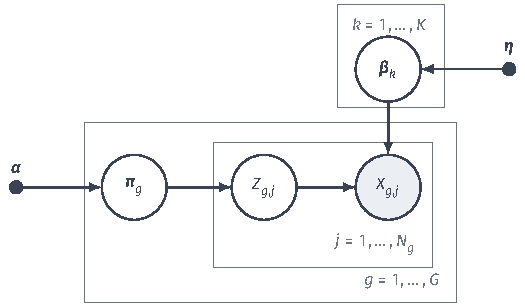
\includegraphics[width=88.935mm]{figures/06-probabilistic-graphical-models/04-models/tikz/pgm-static-directed-plates/figure.pdf}
  \caption{带全局主题先验的LDA重复结构。空心圆表示随机潜在量，填色圆表示观测词，实点表示给定超参数。文档板内每篇有一个$\bm\pi_g$，词板内每词有一组主题分配和观测；$K$个$\bm\beta_k$跨全部文档共享，词节点根据$Z_{g,j}$读取其中一个主题分布。}
  \label{fig:pgm-static-directed-plates}
\end{figure}

若按图~\ref{fig:pgm-static-directed-plates}为主题本身也设置先验，学习对象就改为
\[
 p(\bm\beta_{1:K},\bm\pi_{1:G},\bm z\mid\mathcal D,\bm\alpha,\bm\eta)
 \propto\prod_kp(\bm\beta_k\mid\bm\eta)
      \prod_g p(\bm\pi_g\mid\bm\alpha)
      \prod_{g,j}\pi_{g,z_{g,j}}\beta_{z_{g,j},x_{g,j}}.
\]
这个联合后验保留全局主题的不确定性，不能继续把$\bm\beta$的点参数更新当作同一推断目标。以下用折叠采样直接处理其主题分配。

在主题词分布也有Dirichlet先验的设定下，先积分掉$\bm\pi_g$和$\bm\beta_k$，再使用第~\ref{chap:pgm-sampling}章的Gibbs方法更新一个词的主题。排除当前位置后，文档主题计数记为$n_{g,k}^{-}$，全语料主题词计数为$c_{k,a}^{-}$，并记$c_{k,\cdot}^{-}=\sum_a c_{k,a}^{-}$、$\eta_0=\sum_a\eta_a$，单点条件为
\begin{equation}
  \label{eq:pgm-static-directed-lda-gibbs}
  p(Z_{g,j}=k\mid\text{其余分配},\mathcal{D})
     \propto (n_{g,k}^{-}+\alpha_k)
        \frac{c_{k,x_{g,j}}^{-}+\eta_{x_{g,j}}}
             {c_{k,\cdot}^{-}+\eta_0}.
\end{equation}
文档主题计数给出第一项，主题词计数给出第二项，二者是相应共轭后验的预测权重；文档分母与$k$无关，已经抵消。相乘并归一化，得到精确的单点条件分布。有限轮Gibbs样本构成的整体后验估计仍需考虑抽样误差和混合速度。

实际的一次扫描先从计数表移除当前位置原来的主题贡献，计算式~\eqref{eq:pgm-static-directed-lda-gibbs}的$K$个非负权重，再归一化抽取新主题，并把对应的文档主题计数和主题词计数加回。逐词重复扫描，丢弃初始过渡阶段并检查链的混合后，用保留状态作后验平均。对每个保留分配，可用$\bm\alpha+\bm n_g$与$\bm\eta+\bm c_k$恢复比例和主题的条件Dirichlet后验，再平均所需预测；不能把一个最终分配当成整个后验。

在对称主题先验下，同时置换主题编号和比例坐标，观测分布保持不变。非对称先验可约束部分编号，有限语料中的主题词分布仍可能有其他歧义；相近主题、短文档或过大的主题数会加剧不稳定性。词袋和比例先验各自限制了词序及组间变化，解释主题含义时，需要同时评价这些假设和分解的稳定性。

\subsection{随机成分库及其跨组共享}
\label{sec:pgm-static-directed-random-library}

前面的有限模型先固定可用成分数。现在把总体的成分库也看成未知量：先为一个总体建立随机混合测度，再让多个组共享它提供的原子、拥有不同使用比例。前一个问题由DPM处理，后一个问题再由HDP增加组层；DPM本身仍是单一总体模型。

\subsubsection{DPM：让数据中的占用成分参与推断}
\label{sec:pgm-static-directed-dpm-model}

前面的混合和主题模型都要求事先指定成分（主题）数$K$；$K$过小会欠拟合，过大则浪费容量并增加不稳定性。非参数贝叶斯方法不给成分库设固定上限，而在所有可能成分构成的空间上放置随机概率测度作为先验，使数据实际占用的成分数成为后验推断的一部分。有限混合和主题模型先给定候选成分数$K$。
\term{狄利克雷过程混合}（Dirichlet process mixture, DPM）为混合测度设置随机先验，让有限数据中的占用成分数参与推断。
在标准Borel成分参数空间上，记这个随机概率测度为$G\sim\operatorname{DP}(c,H)$。
其中$c>0$为浓度参数，基测度$cH$的总质量为$c$，$H$是基概率测度。若写作$\operatorname{DP}(\alpha,G_0)$，这里的参数对应为$\alpha=c$、$G_0=H$。
本节采用$c,H$，以区分主题比例先验的参数。
这里需要复用的有限分割规律是：对参数空间的任意有限可测分割$A_1,\ldots,A_m$，随机质量$(G(A_1),\ldots,G(A_m))$服从参数为$(cH(A_1),\ldots,cH(A_m))$的Dirichlet分布；零基质量的单元恒取零。这个规律使计数更新能够同时约束不同分辨率下的成分质量。


无穷多成分、权重总和为1的随机分布不便直接表示，折棒构造（stick-breaking construction）给出一种可数构造：取一根长度为1的棍，第$k$步按一个Beta随机比例从当前剩余棍段上截下一段作为成分$k$的权重，余下部分留给后续成分；反复截取而得的各段长度之和恰为1，由此得到混合建模可用的可数权重序列。
独立抽取$v_k\sim\operatorname{Beta}(1,c)$与$\bm\xi_k\sim H$，依次给剩余质量分配比例$v_k$，令
\[
  w_k=v_k\prod_{\ell<k}(1-v_\ell),\qquad
  G=\sum_{k=1}^{\infty}w_k\delta_{\bm{\xi}_k}.
\]
其中$\delta_{\bm\xi_k}$是原子处的点质量；折棒构造定理保证这个$G$具有上述有限分割规律。
权重和为$1$给出概率测度的归一化，Dirichlet过程分布还依赖这些分割规律。
Teh等的论述介绍了相应构造及其用于层次共享的方式\scite{pgm-static-directed-teh2006}
给定$G$，各记录独立抽取$\bm\zeta_j\mid G\sim G$，再按$\bm X_j\mid\bm\zeta_j\sim p(\cdot\mid\bm\zeta_j)$生成读数。
记录重复抽到一个原子，就使用同一成分参数；成分分布仍可连续。

DPM的学习目标是观测数据下的随机测度和记录分配后验，而非把候选数改大的固定维度最大似然。用$\Pi_{c,H}$表示DP先验律，其目标可写为
\begin{equation}
 p(dG,d\bm\zeta_{1:n}\mid\mathcal D)
 \propto \Pi_{c,H}(dG)\prod_{j=1}^n
       G(d\bm\zeta_j)\,p(\bm x_j\mid\bm\zeta_j).
 \label{eq:pgm-static-directed-dpm-posterior}
\end{equation}
给定读数时，占用成分的证据同时来自已有计数与该成分能否解释当前读数。下面先在成分参数已知的条件下计算DP更新，再把这个结果用于数据条件下的分配。

给定$n$个潜在成分参数，在任意有限分割上，用各单元的计数更新Dirichlet先验。
把这些相容的分割更新合在一起，得到随机测度的后验
\[
  G\mid\bm\zeta_{1:n}\sim\operatorname{DP}
    \left(c+n,\frac{cH+\sum_{j=1}^n\delta_{\bm\zeta_j}}{c+n}\right).
\]
下一条记录的成分参数预测分布由这个后验的均值给出。

取无原子的$H$并积分掉$G$，前$n$个潜在参数中占用成分$k$的计数为$n_k$，下一条复用它的概率为$n_k/(n+c)$，新抽成分的总概率为$c/(n+c)$。已有计数$(3,1)$、$c=1$时，三个选择分别为$0.6,0.2,0.2$。若该条读数也已给定，还需乘各已有成分和基准测度下的预测密度，再归一化。有限$n$至多占用$n$个成分，第$j$次增加成分的先验概率为$c/(c+j-1)$，所以占用数的先验期望是这些概率之和$\sum_{j=1}^n c/(c+j-1)$。可数先验放宽候选容量，实际推断处理当前占用或截断的候选成分，恢复真实有限类别数还需要其他条件。

在$H$与成分似然共轭的情形，可以积分掉$G$及各成分参数，直接更新记录的成分编号。把第$j$条记录移出后，令$n_k^{-j}$为剩余第$k$组的记录数，$\mathcal D_k^{-j}$为其数据。已有成分与新成分的未归一化权重分别是
\begin{equation}
 \begin{aligned}
 a_k&=n_k^{-j}\int p(\bm x_j\mid\bm\xi)
                              p(d\bm\xi\mid\mathcal D_k^{-j}),\\
 a_{\mathrm{new}}&=c\int p(\bm x_j\mid\bm\xi)H(d\bm\xi).
 \end{aligned}
 \label{eq:pgm-static-directed-dpm-allocation}
\end{equation}
先删除移出后变空的成分，再计算各预测密度、归一化这些权重并抽取新编号，最后写回计数与充分统计量；若选中新成分，则创建相应统计量。反复扫描得到占用数和预测分布的后验近似，成分参数需要时再从对应条件后验抽取。这说明$c/(n+c)$只是尚未读取新观测时的新建概率，不能直接用作给定读数后的分配概率。非共轭成分的预测积分可能不能解析完成，须再用数值积分、辅助变量或其他近似，并检查相应采样方法的有效性。

\subsubsection{HDP：使多个组共享同一套可数成分}
\label{sec:pgm-static-directed-hdp-model}

DPM解决了单组数据下成分数不定的问题，但在多组（多篇文档、多个工厂）场景下还有新问题：我们希望各组\emph{共享同一套}主题或成分，只是使用比例不同——不同文档讨论的应是同一批主题，而不是每篇文档各发明一套。若给每组单独抽一个Dirichlet过程，由于基测度连续，各组抽到的成分几乎必然互不相同，无法共享。解决办法是在组之上再加一层：先抽一个全局的随机成分库，再让每组的随机测度围绕这个全局库生成。多个组需要共享成分时，还要让它们使用相同原子。从同一个无原子$H$分别抽取独立Dirichlet过程，各组的原子几乎必然不同。\term{层次狄利克雷过程}（hierarchical Dirichlet process, HDP）取全局浓度参数$\gamma>0$，先抽离散的随机基准，再由它生成组测度：
\begin{equation}
  \label{eq:pgm-static-directed-hdp}
  G_0\sim\operatorname{DP}(\gamma,H),\qquad
  G_g\mid G_0\sim\operatorname{DP}(c,G_0).
\end{equation}
$G_0$几乎必然离散，所以各$G_g$共用同一可数原子集合，同时分别具有组级权重。在主题模型中，这些原子是词分布，每篇文档按自己的权重逐词选择共享主题。一个模型因此同时具有层次共享、混合成员及非固定成分数；这些属性描述不同的组织方式。Teh等进一步说明DP构造和HDP共享原子的机制\scite{pgm-static-directed-teh2006}

HDP的完整生成结构还包括$\bm\zeta_{g,j}\mid G_g\sim G_g$和$X_{g,j}\mid\bm\zeta_{g,j}\sim p(\cdot\mid\bm\zeta_{g,j})$。固定$c,\gamma,H$时，学习目标是全局测度、组测度及各项成分参数的联合后验：
\begin{equation}
 \begin{aligned}
 &p(dG_0,dG_{1:G},d\bm\zeta\mid\mathcal D)\\
 &\quad\propto\Pi_{\gamma,H}(dG_0)
     \prod_g\Pi_{c,G_0}(dG_g)
     \prod_{g,j}G_g(d\bm\zeta_{g,j})p(x_{g,j}\mid\bm\zeta_{g,j}).
 \end{aligned}
 \label{eq:pgm-static-directed-hdp-posterior}
\end{equation}
这里$G$在下标范围$1{:}G$中表示组数，$G_g$表示第$g$组的随机测度。条件于全局库，各组独立抽取权重；观测却会通过未知的全局库联系各组后验。与LDA相比，HDP既推断哪些主题被占用，也推断全局使用倾向怎样约束各文档比例，不能只把它理解为给固定主题数的LDA多加一个普通先验。

为把这个目标变成有限计算，下面在主题词模型中构造一个明确的截断近似。固定截断数$K$，取$v_k\sim\operatorname{Beta}(1,\gamma)$（$k<K$）并令$v_K=1$，把剩余折棒质量合并到最后一项，定义$w_k=v_k\prod_{\ell<k}(1-v_\ell)$。共享原子$\bm\xi_k$在这里是词概率向量，取$H=\operatorname{Dirichlet}(\bm\eta)$。每篇文档的组权重为$\bm\pi_g\mid\bm w\sim\operatorname{Dirichlet}(c\bm w)$，再按$Z_{g,j}\sim\operatorname{Categorical}(\bm\pi_g)$、$X_{g,j}\sim\operatorname{Categorical}(\bm\xi_{Z_{g,j}})$生成词。这个有限模型基于共享原子表示，但$K$有限时不同于原来的可数HDP，必须保留截断敏感性检查。

记全部未知量为$\Omega=(\bm v,\bm\xi,\bm\pi,\bm z)$，上述步骤对应明确的联合密度
\begin{equation}
 \begin{aligned}
 p_K(\mathcal D,\Omega)
 ={}&\prod_{k<K}\operatorname{Beta}(v_k;1,\gamma)
       \prod_{k=1}^K\operatorname{Dirichlet}(\bm\xi_k;\bm\eta)\\
 &\cdot\prod_g\operatorname{Dirichlet}(\bm\pi_g;c\bm w)
       \prod_{g,j}\pi_{g,z_{g,j}}\xi_{z_{g,j},x_{g,j}}.
 \end{aligned}
 \label{eq:pgm-static-directed-hdp-truncated-joint}
\end{equation}
采用平均场$q(\Omega)=\prod_{k<K}q(v_k)\prod_kq(\bm\xi_k)\prod_gq(\bm\pi_g)\prod_{g,j}q(Z_{g,j})$，其中折棒因子为Beta，词分布与组权重因子为Dirichlet，分配因子为类别分布。所有形状参数保持正值。具体的优化目标是
\begin{equation}
 \max_q\;\mathcal L_K(q)
   =\mathbb E_q[\log p_K(\mathcal D,\Omega)-\log q(\Omega)].
 \label{eq:pgm-static-directed-hdp-elbo}
\end{equation}
它下界化的是有限模型的$\log p_K(\mathcal D)$；提高该下界不能直接证明原可数模型的证据提高。这里把第~\ref{chap:pgm-variational}章的变分原理用于刚才写出的有限联合模型，不把以下计算称为原HDP的解析后验。

令$q(\bm\pi_g)=\operatorname{Dirichlet}(\bm a_g)$、$q(\bm\xi_k)=\operatorname{Dirichlet}(\bm\lambda_k)$、$q(Z_{g,j}=k)=r_{g,j,k}$。固定其余因子时，分别收集联合对数密度中含当前变量的项，可得
\begin{equation}
 \begin{aligned}
 r_{g,j,k}&\propto\exp\{\mathbb E_q\log\pi_{g,k}
                          +\mathbb E_q\log\xi_{k,x_{g,j}}\},\\
 a_{g,k}&=c\mathbb E_q[w_k]+\sum_jr_{g,j,k},\\
 \lambda_{k,a}&=\eta_a+\sum_{g,j}r_{g,j,k}\mathbb I\{x_{g,j}=a\}.
 \end{aligned}
 \label{eq:pgm-static-directed-hdp-local-vi}
\end{equation}
第一行对$k$归一化；两类对数期望与LDA一样由digamma差计算。组权重更新的先验伪计数是$c\mathbb E_q[w_k]$，而不是每组各自固定的一组$\alpha_k$；共享主题更新则汇集所有文档的词频。若$q(v_k)=\operatorname{Beta}(u_k,b_k)$，独立性给出$\mathbb E_q[w_k]=\mathbb E_q[v_k]\prod_{\ell<k}\mathbb E_q[1-v_\ell]$，其中$\mathbb E_q[v_k]=u_k/(u_k+b_k)$、$v_K=1$。

全局折棒的更新不能直接套用LDA计数公式。组先验的对数密度中包含以下依赖全局权重的项：
\[
 -\sum_k\log\Gamma(cw_k).
\]
它使全局权重与组权重之间不再共轭。固定其他变分因子后，可对Beta形状参数的对数$\bm\omega=(\log u_k,\log b_k)_{k<K}$数值优化$\mathcal L_K$。例如把其他因子的期望先汇总，记$A(\bm v)=\mathbb E_{q(\Omega\setminus\bm v)}\log p_K(\mathcal D,\Omega)$，在微分与积分可交换、梯度估计方差有限时，有
\[
 \nabla_{\bm\omega}\mathcal L_K
 =\mathbb E_{q_{\bm\omega}(\bm v)}
 [(A(\bm v)-\log q_{\bm\omega}(\bm v))
                     \nabla_{\bm\omega}\log q_{\bm\omega}(\bm v)].
\]
抽取折棒样本、计算括号内的全局与组先验项，再平均梯度并更新$\bm\omega$，就是前文评分函数估计在这个模型中的一项实现。概率接近边界时要检查数值精度和梯度方差；有限样本梯度更新不保证每一步ELBO上升。

完整训练循环因而包含：更新各词分配，汇总组权重与共享主题的参数，再优化全局折棒因子；随后回到各文档重算分配。初始化时使用正的形状参数，局部更新可多次迭代；停止时同时检查ELBO估计的变化及其蒙特卡洛波动，而不是仅比较相邻两次带噪数值。增大$K$后重新检查预测和尾部质量敏感性，分别报告截断近似、平均场近似与数值优化的限制。给已有文档预测新词，可用$\sum_k\mathbb E_q[\pi_{g,k}]\mathbb E_q[\xi_{k,a}]$；新文档则先从学得的全局权重及共享主题构造组先验，再结合其已观测词做局部推断。

DPM和HDP把有限数据占用的成分数、分配与随机权重纳入后验推断。以上演示固定浓度等超参数；若还要估计这些量，需要另加经验贝叶斯目标，或为它们设先验后扩大联合后验。截断变分用有限候选近似可数模型，需要检查截断误差；采样调整占用成分，需要检查链的混合。HDP还要共同处理组级成分和全局原子的关系，独立拟合各组有限混合无法完成这项共享推断。浓度参数影响分组倾向，需结合超参数估计和预测检验使用。输出时可报告预测、占用数及组间共享的不确定性，原子编号本身仍只承担命名。

\section{结构组合与查询选择}
\label{sec:pgm-static-directed-comparison}

本章模型沿两个维度变化：潜变量取值离散或连续，共享发生在记录内或跨组。比较时固定三条线索：面对一个查询，模型要对哪些随机量求和或积分、这些量在什么范围内共享、哪些非唯一性会限制对结果的解释；先固定查询与被积分的随机量，才能在同一口径下比较计算代价和适用场景。在表~\ref{tab:pgm-static-directed-comparison}中，给定所选全局参数或超参数，按各模型的设定汇总随机潜在量，得到观测似然$p(\bm x)$；用点估计固定的参数不再积分。NB和TAN的完整训练记录为$(y,\bm x)$，类别预测时则对$Y$归一化。独立性、共享和非唯一性另列，便于分析同一种查询在不同结构中需要完成哪些工作。

\begin{table*}[htbp]
  \centering
  \small
  \begin{tabularx}{\linewidth}{@{}
    >{\raggedright\arraybackslash}p{28mm}
    >{\raggedright\arraybackslash}p{30mm}
    >{\raggedright\arraybackslash}p{27mm}
    >{\raggedright\arraybackslash}p{30mm}
    >{\raggedright\arraybackslash}X@{}}
    \toprule
    模型与潜在量 & 独立性与共享 & 观测似然 & 局部后验 & 非唯一性与主要代价\\
    \midrule
    NB／TAN：训练时无潜变量 &
    类内独立／类内树；参数跨样本共享 &
    完整记录直接乘积 &
    类别后验枚举$K$项 &
    支持不足的条件表不确定；TAN还需选择树\\
    自回归：无随机潜变量 &
    顺序父集；条件网络可共享参数 &
    条件密度直接乘积 &
    前缀续写直接；任意补全未必易算 &
    网络参数可不唯一；优化、顺序选择与串行生成\\
    有限混合：离散分配 &
    样本在固定参数下独立；类内结构由成分决定 &
    $K$项有限和 &
    成分责任度精确 &
    标签交换、冗余成分；局部极值与退化\\
    FA／PPCA：连续因子 &
    给定因子后观测独立；共享载荷 &
    解析高斯密度 &
    解析高斯后验与缺失预测 &
    旋转及可能的额外分解歧义；维数与噪声假设\\
    LDA：连续比例与离散主题 &
    组级比例、全局主题；组内条件独立 &
    需积分比例，通常近似 &
    联合后验通常近似，局部条件可解析 &
    主题置换与重叠；局部推断和全局学习交替\\
    DPM／HDP：分配与随机测度 &
    可数候选成分；HDP跨组共享原子 &
    对未知随机量积分通常需近似 &
    采样或截断变分 &
    成分编号不唯一；占用数、超参数与近似误差\\
    \bottomrule
  \end{tabularx}
  \caption{静态有向模型在给定参数或超参数下的计算。表中的精确结果指相应有限求和、解析积分或局部条件；学习目标、参数不确定性及潜在解释另按各模型分析。}
  \label{tab:pgm-static-directed-comparison}
\end{table*}

直接模型以局部条件拟合观测联合分布。NB用类内独立减少待估参数，TAN增加树边及结构搜索，神经自回归则用非线性条件与参数共享扩大可表达的关系。完整记录可直接计算局部乘积，祖先生成和缺失查询还需按各自依赖进行。潜变量路线也可能保留精确计算：有限混合显式汇总$K$项，线性高斯模型解析积分，同时给出似然和局部后验。

共享随机量会联系不同位置的推断。pLSA固定文档比例时，逐词做有限求和；LDA积分共同的文档比例后，主题分配需要一起解释这些词。全局主题再带先验时，不同文档也相互联系，HDP还需要推断共享的占用成分。这些联系决定了联合后验的规模，除各变量的状态数外，还需考察它们共同读取哪些数据。

模型之间的联系还要落到结构和学习对象的变化上。NB与TAN都保留类别生成属性的结构，TAN只放宽类内父集；把NB的训练类别隐藏，并保留原来的条件乘积，就得到乘积分布的有限混合。这里改变的是类别的观测状态，所以已知计数变成需要E步计算的后验期望计数。FA到PPCA则没有改变观测状态，而是把逐维噪声约束为同一个方差；两者都约束协方差的低秩加噪声分解。下一章的高斯马尔可夫随机场将转而约束精度矩阵的零元素，二者对同一高斯分布族施加不同结构限制。自回归网络的三种实现都保留顺序条件乘积，掩码和卷积改变条件函数的计算及参数共享。

有限混合与混合成员的区别在分配单位：前者一条记录选择一个成分，后者在一组内部逐项选择。pLSA到LDA进一步把文档比例由固定参数变为随机量，因此新文档有了比例先验，也增加了比例积分。DPM对单一总体引入随机成分库；HDP在这个库之上增加组权重，让不同组共享原子而保持不同使用比例。这些变化分别作用于容量、共享和分配单位，不能排成一条每个模型都替代前者的升级链。

表~\ref{tab:pgm-static-directed-learning-map}补充各分支的目标和更新对象，与表~\ref{tab:pgm-static-directed-comparison}的查询成本合读，可以区分“模型怎样表示”“参数怎样学到”和“训练后怎样使用”。
\begin{table*}[htbp]
 \centering\small
 \begin{tabularx}{\linewidth}{@{}p{25mm}XXX@{}}
 \toprule
 模型 & 结构改变与动机 & 学习目标 & 具体更新对象\\
 \midrule
 NB／TAN & 类内独立或属性树减少条件表规模 & 带标签联合似然；TAN另选树 & 类别与父配置计数；条件互信息最大生成树\\
 NADE／MADE／PixelCNN & 前缀复用、掩码与空间共享控制条件函数 & 完整记录自回归负对数似然 & 由各位置梯度共同更新网络权重\\
 有限混合／GMM & 用未知离散成分解释多种模式 & 成分求和后的观测似然 & 责任度、加权均值与协方差交替更新\\
 FA／PPCA & 连续共同强度与独有噪声分解相关 & 低秩加噪声高斯似然 & 后验一、二阶矩，载荷与受约束噪声\\
 层次正态 & 组参数共享总体且保留差异 & 组边缘似然或联合后验 & 组后验矩与超参数；或联合采样、变分\\
 pLSA／LDA & 逐词分配；固定或随机文档比例 & pLSA似然、LDA的ELBO或联合后验 & 文档比例、主题词频；LDA另推断比例或折叠分配\\
 DPM／HDP & 随机成分库；HDP跨组共享原子 & 随机测度联合后验；有限近似的ELBO & 分配、成分、组权重及全局权重\\
 \bottomrule
 \end{tabularx}
 \caption{建模选择与学习计算的对应。表中并列的目标属于不同设定，使用某一模型时须先选定点参数估计或贝叶斯后验目标，再采用相应更新。}
 \label{tab:pgm-static-directed-learning-map}
\end{table*}

也可以组合上述属性。混合因子分析为每个离散成分配置连续因子，成分内积分后仍是低秩加对角协方差的高斯，所以成分责任度和因子后验可解析计算。自回归条件可采用有限混合，组级载荷可设置层次先验。因此离散或连续、线性高斯或非线性、组间共享或独立、逐项生成或联合生成，分别描述模型的一项选择。

观测分布估计准确时，潜在解释仍可能受对称性约束：网络权重可有多种表示，成分可交换编号，因子可旋转方向。选择模型时，可先用留出数据评价预测，再按目的检查所需输出；解释结构需要报告对称性及稳定性，补全任务则需要评价条件预测和误差范围。似然计算、预测表现和潜在语义各有相应的核验对象。

\section{本章小结}
\label{sec:pgm-static-directed-summary}

本章把表示、推断和学习组装到具体的静态有向模型上，并沿三条主线展开：观测之间的直接依赖、记录内部由潜变量给出的共同解释、以及跨记录跨组的共享。静态有向分解把局部条件组合成联合分布。全部变量可观测时直接读取乘积，引入潜在状态后则先汇总它们，得到观测分布。两个传感器的同一联合表可用自回归条件或隐藏类别的混合表示，前者给出读数预测次序，后者加入需要另行验证的工作状态解释。

有限混合用责任度与成分参数交替学习，固定参数的局部后验仍可精确求得。线性高斯积分把观测协方差、降维和缺失预测联系起来；共享随机量与混合成员联系多个记录或组的推断，联合计算可能需要近似。取值类型与共享方式可以组合使用，标签置换、因子旋转和其他分解歧义则限制了潜在坐标的唯一解释。

判断新模型时，可以从联合归一化、查询待消变量、共享范围和估计的边界条件逐项展开。若建模依据首先是变量状态之间的相容性，可以改用局部相容函数与统一归一化，而不必先指定谁生成谁。第~\ref{chap:pgm-energy-models}章据此比较联合归一化与输出条件归一化；这是一种表示选择，不意味着有向分解不能表达对称的观测分布。第~\ref{chap:pgm-generative}章再以自回归和高斯潜变量为参照，讨论神经网络如何参数化更灵活的密度，以及相应概率计算的代价。

\paragraph{扩展阅读}
Bishop的PRML用混合、潜变量及变分学习展开静态模型，Koller与Friedman从局部条件结构讨论共同的推断与学习方法。可沿同一图的作用域比较不同局部分布，检查哪些求和或积分仍有解析形式，哪些学习目标需要近似后验\scite{bishop2006,pgm-koller2009}

\chapter{静态无向模型}
\label{chap:pgm-energy-models}

相邻检测位置可能同时过热，也可能受到同一测量干扰，整排状态因而需要联合考虑。给定各位置的相对偏好以及相邻状态的相容权重，怎样计算整排配置的概率？若温度读数已知、只需预测异常标签，是否还要同时建立这些读数的生成分布？

两项任务都可以组合局部势，区别在于哪些变量参与归一化。联合无向模型比较全部建模变量的配置，条件无向模型则固定输入、只比较输出。局部无向分解规定了变量在给定分隔节点后的独立关系（参见第~\ref{chap:pgm-undirected}章）；本章据此构造具体模型，说明结构怎样影响推断，以及潜变量、高阶势和神经参数化各带来哪些表达能力与计算要求。联合与条件是本章的主要划分；变量是否可见、势是否成对以及参数化方式可以组合。

\section{无向模型的共同形式}
\label{sec:pgm-energy-models-common}

先为整排状态规定无向图$\mathcal{G}=(V,E)$，令$d=|V|$、$\bm{X}=(X_1,\ldots,X_d)^\top$。局部配置越符合建模偏好，其\term{势函数}（potential function）值越大；这个值表示相对相容程度，无须自身求和为$1$。记因子作用域集合为$\mathcal{C}$，每个$C\in\mathcal{C}$取图中的一个团，允许使用非极大团。将严格正势$\psi_{\bm{\theta},C}$写成局部能量$E_{\bm{\theta},C}=-\log\psi_{\bm{\theta},C}$，乘积权重便转为能量之和：
\begin{equation}
  \begin{aligned}
    E_{\bm{\theta}}(\bm{x})
      &=\sum_{C\in\mathcal{C}}E_{\bm{\theta},C}(\bm{x}_C),\\
    p_{\bm{\theta}}(\bm{x})
      &=\frac{\prod_{C\in\mathcal{C}}
               \psi_{\bm{\theta},C}(\bm{x}_C)}
              {Z_{\bm{\theta}}}
        =\frac{\exp[-E_{\bm{\theta}}(\bm{x})]}{Z_{\bm{\theta}}},\\
    Z_{\bm{\theta}}
      &=\int \exp[-E_{\bm{\theta}}(\bm{u})]\,\mathrm{d}\mu(\bm{u}).
  \end{aligned}
  \label{eq:pgm-energy-models-joint}
\end{equation}
参数向量$\bm{\theta}$包含各局部势的参数。离散状态采用计数测度$\mu$，连续状态采用指定基准测度，通常是Lebesgue测度。\term{能量函数}（energy function）的值越低，配置的未归一化权重越大；\term{配分函数}（partition function）$Z_{\bm{\theta}}$累加或积分全部权重，使其成为概率，故须满足$0<Z_{\bm{\theta}}<\infty$。这里使用无量纲的对数权重，物理模型的逆温度已计入参数。

也可以用负能量$f_{\bm{\theta}}=-E_{\bm{\theta}}$给配置评分，对数概率还需扣除$\log Z_{\bm{\theta}}$。增加与$\bm{x}$无关的能量常数，会等比例缩放全部权重及配分函数，概率保持原值。按正比例缩放能量时，配置间的能量差也同比例变化；比例不为$1$且两个配置的能量不同时，它们的概率比会改变。若只比较固定模型中的两种配置，配分函数可从比值中消去：
\[
  \frac{p_{\bm{\theta}}(\bm{x})}{p_{\bm{\theta}}(\bm{x}')}
  =\exp\{E_{\bm{\theta}}(\bm{x}')-E_{\bm{\theta}}(\bm{x})\}.
\]
因此，能量差能够排序配置，绝对概率仍依赖全部权重的总量。改变局部势的状态偏好时，配分函数也可能改变；即使某个配置的未归一化权重不变，其概率仍可能随归一化而改变。

若测量输入$\bm{x}$已经固定、待预测量为$\bm{Y}$，需要比较的候选只有输出配置。相同能量构造此时只在输出空间归一化：
\begin{equation}
  \begin{aligned}
    p_{\bm{\theta}}(\bm{y}\mid\bm{x})
      &=\frac{\exp[-E_{\bm{\theta}}(\bm{y},\bm{x})]}
              {Z_{\bm{\theta}}(\bm{x})},\\
    Z_{\bm{\theta}}(\bm{x})
      &=\int\exp[-E_{\bm{\theta}}(\bm{v},\bm{x})]
                  \,\mathrm{d}\mu_Y(\bm{v}).
  \end{aligned}
  \label{eq:pgm-energy-models-conditional}
\end{equation}
每个使用的输入都须给出$0<Z_{\bm{\theta}}(\bm{x})<\infty$。该式只定义输出的条件概率，没有为输入规定$p(\bm{x})$，也不限制输入之间的依赖。附加只依赖输入的能量$c(\bm{x})$时，它在分子、分母中消去。图~\ref{fig:pgm-energy-models-normalization}据此区分输入的两种职责：它可以改变各势的数值，却不参与输出的求和。

\begin{figure}[htbp]
  \centering
  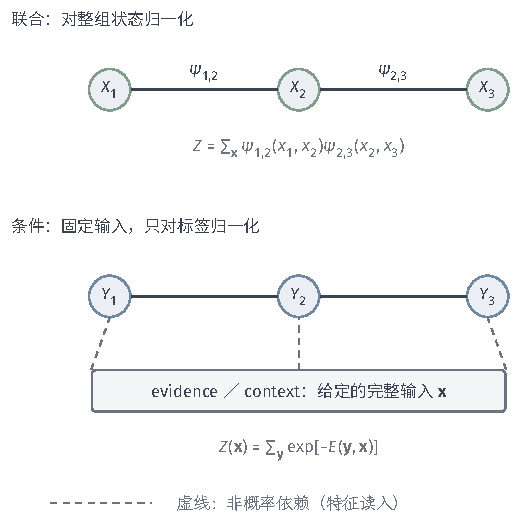
\includegraphics[width=86.907mm]{figures/06-probabilistic-graphical-models/04-models/tikz/pgm-energy-models-normalization/figure.pdf}
  \caption{三节点相互作用的两种归一化。上方联合模型对全部状态求和；下方把$\bm{x}$列为给定证据或条件输入，只对标签$\bm{y}$求和。灰底框中的输入通过虚线影响标签势，虚线表示特征依赖，不表示有向生成关系。}
  \label{fig:pgm-energy-models-normalization}
\end{figure}

有限离散状态配合有限能量，必然产生正且有限的配分函数。连续能量则需检查尾部：即使$E(x)=-x^2$处处有定义，$\int_{\mathbb{R}}e^{x^2}\,\mathrm{d}x$仍发散。允许势为零时，可以用$+\infty$能量排除配置，但归一化还须有正总权重；离散支持至少保留一个正权配置，连续支持则需有正测度。因子分解仍能给出相应Markov性质，而从Markov性质反推分解的正性定理不能直接用于零势（参见第~\ref{chap:pgm-undirected}章）。

\section{联合能量模型}
\label{sec:pgm-energy-models-joint-models}

为整组测量状态建立联合分布，可以用于补全状态、计算多变量事件概率或生成配置。以下先取成对作用，再分别引入隐藏状态、改变能量函数或扩大因子作用域。它们共同使用式~\eqref{eq:pgm-energy-models-joint}，推断时能利用的分解与代数形式却各不相同。

\subsection{观测变量成对模型}
\label{sec:pgm-energy-models-pairwise}

对只有两种状态的检测位置，取$x_i\in\{-1,+1\}$。\term{Ising模型}（Ising model）分别用单点参数表示状态偏好，用边参数表示相邻状态同号或异号的偏好：
\begin{equation}
  E_{\bm{\theta}}(\bm{x})
    =-\sum_{i\in V}b_ix_i
     -\sum_{\{i,j\}\in E}J_{i,j}x_ix_j.
  \label{eq:pgm-energy-models-ising}
\end{equation}
\term{外场}（external field）$b_i$取正值时偏好$+1$。\term{耦合参数}（coupling parameter）$J_{i,j}$取正值时奖励同号，取负值时奖励异号；每条无向边只计一次，约定$J_{i,j}=J_{j,i}$。这些参数描述统计相容性，不能仅凭它们推断干预一个位置对另一位置的效应。

要计算一个位置的条件概率，固定其余状态，仅保留含$x_i$的得分$x_i(b_i+\sum_{j\in N(i)}J_{i,j}x_j)$，其中$N(i)$为邻居集合。$+1$与$-1$的权重比为$\exp[2(b_i+\sum_jJ_{i,j}x_j)]$，归一化两项后得到
\begin{equation}
  \begin{aligned}
    p_{\bm{\theta}}(X_i=+1\mid\bm{x}_{V\setminus\{i\}})
      &=\sigma\!\left(2b_i+
           2\sum_{j\in N(i)}J_{i,j}x_j\right),\\
    \sigma(u)&=\frac{1}{1+e^{-u}}.
  \end{aligned}
  \label{eq:pgm-energy-models-ising-conditional}
\end{equation}
这个满条件分布只读取邻居状态。移去这些条件以后，无直接边的两个节点仍可能经其他节点相关。

用三个相邻位置构造数值例子：图取$1-2-3$，不设单点偏好，同号边势为$3$、异号边势为$1$。这些是人为指定的权重，尚未归一化为概率。为计算联合权重，先统计相邻同号对：
\[
  N_{=}(\bm{x})
   =\mathbf{1}\{x_1=x_2\}+\mathbf{1}\{x_2=x_3\}.
\]
令$E_0(\bm{x})=-(\log3)N_{=}(\bm{x})$，配置权重就是$3^{N_{=}(\bm{x})}$。首节点可取两个值，每个后继节点的两项权重和为$3+1=4$，故$Z_0=2\times4\times4=32$。由$\mathbf{1}\{x_i=x_j\}=(1+x_ix_j)/2$，这也对应$J_{1,2}=J_{2,3}=(\log3)/2$的Ising分布。两种能量约定相差常数：$E_0$比式~\eqref{eq:pgm-energy-models-ising}的零外场能量少$\log3$，后者的配分函数为$32/3$。概率相同，配分函数数值则随能量常数而变。

在该对称链中，给定一个位置，后继位置同号和异号的条件概率分别为$3/4$、$1/4$。两端同号对应两次保持或两次翻转，因而
\[
  p(X_3=X_1\mid X_1)
    =(3/4)^2+(1/4)^2=\frac58.
\]
各节点的边缘都为均匀二值分布，所以$\mathbb{E}[X_1X_3]=2(5/8)-1=1/4$。两端虽无边仍相关，给定$X_2$才独立。将同样参数用于更长的零外场链，每跨一条边，条件均值乘以$1/2$，相隔$r$条边的相关为$(1/2)^r$。这说明相互作用能够沿路径传递，其强度还由参数决定。

类别数增加到$K>2$后，标签编号的乘积无法直接表示相容性。\term{Potts模型}（Potts model）改为比较类别是否相等，对$x_i\in\{1,\ldots,K\}$定义
\begin{equation}
  E_{\bm{\theta}}(\bm{x})
   =-\sum_i b_i(x_i)
    -\sum_{\{i,j\}\in E}J_{i,j}\mathbf{1}\{x_i=x_j\}.
  \label{eq:pgm-energy-models-potts}
\end{equation}
$b_i(k)$规定位置$i$对类别$k$的偏好。计算节点条件分布时，固定邻居，为每个类别$k$形成权重
\[
  w_i(k)=\exp\left\{
    b_i(k)+\sum_{j\in N(i)}J_{i,j}\mathbf{1}\{k=x_j\}
  \right\},
\]
将权重除以$\sum_{\ell=1}^K w_i(\ell)$即得满条件概率。每条边只用一个参数区分类别相同与不同，限制了它能表达的相容关系；特定异类组合有不同偏好时，需改用$K\times K$边势表。二类Potts可以重新编码为Ising，其中耦合系数需按前述$1/2$因子换算。

完整观测提供单点状态以及边上的乘积或同类指示。固定图、存在有限内点最大似然解时，模型期望与对应经验统计量匹配；例如$J_{i,j}$的似然梯度使用经验$x_ix_j$减去$\mathbb{E}[X_iX_j]$（通用推导及替代准则参见第~\ref{chap:pgm-parameter-learning}章）。Ising的解析满条件还能直接用于Gibbs更新和伪似然拟合。强耦合时，单点变化难以转到另一种整体配置，采样仍可能很慢。

一般稠密边势在树上求配分函数与边缘需$O(dK^2)$运算，特殊边势可能进一步简化。一般图则受消元后的诱导宽度限制，原始因子成对不保证全局计算只有二次成本。二值吸引型模型可以通过图割求最优配置，但这一最大化未计算配分函数（参见第~\ref{chap:pgm-variational}章）。参数也会限制模型适用性：过强的同号偏好可能掩盖局部异常；三角形的每条边都偏好异号时，任一二值配置至少违背一项偏好。

温度等连续状态可以用二次能量描述。\term{高斯Markov随机场}（Gaussian Markov random field, GMRF）通过精度矩阵表示条件依赖；对$\bm{x}\in\mathbb{R}^d$取
\begin{equation}
  \begin{aligned}
    E_{\bm{\theta}}(\bm{x})
      &=\frac12(\bm{x}-\bm{\mu})^\top
                    \bm{Q}(\bm{x}-\bm{\mu}),\\
    Z_{\bm{\theta}}
      &=(2\pi)^{d/2}|\bm{Q}|^{-1/2},
      \qquad \bm{Q}=\bm{Q}^\top\succ0.
  \end{aligned}
  \label{eq:pgm-energy-models-gaussian}
\end{equation}
均值为$\bm{\mu}$，协方差的逆$\bm{Q}$称为\term{精度矩阵}（precision matrix）。正定性使二次能量在所有方向增长，并使高斯积分有限。为补全一个未知位置，给定其余位置后的分布为
\[
  \begin{aligned}
    \widetilde{\mu}_i(\bm{x})
      &=\mu_i-\frac{1}{Q_{i,i}}
           \sum_{j\ne i}Q_{i,j}(x_j-\mu_j),\\
    X_i\mid\bm{x}_{V\setminus\{i\}}
      &\sim\mathcal{N}\!\left(
          \widetilde{\mu}_i(\bm{x}),Q_{i,i}^{-1}\right).
  \end{aligned}
\]
$\widetilde{\mu}_i$是给定其余节点后的条件均值。在非退化高斯模型中，$Q_{i,j}=0$恰好对应$X_i\perp X_j\mid\bm{X}_{V\setminus\{i,j\}}$；协方差为零判别的则是边缘独立，两者不可互换（证明参见第~\ref{chap:pgm-undirected}章）。

仍取三个检测位置，用中心化并缩放后的温度构造零均值模型，令
\[
  \bm{Q}=
  \begin{pmatrix}
    2&-1&0\\ -1&2&-1\\ 0&-1&2
  \end{pmatrix},
  \qquad
  \bm{Q}^{-1}=\frac14
  \begin{pmatrix}
    3&2&1\\ 2&4&2\\ 1&2&3
  \end{pmatrix}.
\]
$\bm{Q}$的顺序主子式为$2,3,4$，所以它正定。两端精度为零，协方差却为$1/4$，展示了中点传递的边缘相关。给定$x_1=2,x_3=0$，中点分布为$\mathcal{N}(1,1/2)$；以条件均值补全得到$1$，条件方差则量化补全后仍有的不确定性。

高斯推断主要使用线性求解和矩阵分解。稠密Cholesky分解耗时$O(d^3)$，随后可计算条件均值、所需协方差及对数行列式；链状精度具有固定带宽时，分解可随$d$线性增长。一般稀疏矩阵可能产生消元填充，原始零元素数量因此不足以判定时间成本。学习时，若均值已知为零，取样本二阶矩$\bm{S}=n^{-1}\sum_{r=1}^n\bm{x}_r\bm{x}_r^\top$，要最大化的精度相关对数似然为
\[
  \frac n2\{\log|\bm{Q}|-\operatorname{tr}(\bm{S}\bm{Q})\},
  \qquad \bm{Q}\succ0,
\]
缺边对应$Q_{i,j}=0$，这些约束与正定性共同限定候选精度。无图约束且$\bm{S}\succ0$时，最优解是$\bm{S}^{-1}$；有零约束时通常需要约束优化。仅半正定的精度不能在整个$\mathbb{R}^d$上归一化为式~\eqref{eq:pgm-energy-models-gaussian}，单个高斯也无法表达多峰。解析计算的便利伴随这些表示条件，延长优化迭代不能消除它们\scite{pgm-undirected-rue2005}

\subsection{潜变量能量模型}
\label{sec:pgm-energy-models-latent}

共同异常也可能来自未测状态。可以让一个潜变量连接多个可见位置，先建立联合分布，再将它边缘化。\term{玻尔兹曼机}（Boltzmann machine, BM）采用二值变量的成对能量实现这一构造。以下改用$0/1$编码：可见量为$\bm{x}\in\{0,1\}^{d_{\mathrm{v}}}$，隐藏量为$\bm{z}\in\{0,1\}^m$，共有$d_{\mathrm{v}}+m$个节点：
\begin{equation}
  \begin{aligned}
    E_{\bm{\theta}}(\bm{x},\bm{z})
      &=-\bm{b}^\top\bm{x}-\bm{c}^\top\bm{z}
        -\bm{x}^\top\bm{W}\bm{z}\\
      &\quad-\frac12\bm{x}^\top\bm{U}\bm{x}
             -\frac12\bm{z}^\top\bm{R}\bm{z},\\
    p_{\bm{\theta}}(\bm{x},\bm{z})
      &=\frac{e^{-E_{\bm{\theta}}(\bm{x},\bm{z})}}
               {Z_{\bm{\theta}}},\\
    p_{\bm{\theta}}(\bm{x})
      &=\sum_{\bm{z}}p_{\bm{\theta}}(\bm{x},\bm{z}).
  \end{aligned}
  \label{eq:pgm-energy-models-bm}
\end{equation}
$\bm{W}\in\mathbb{R}^{d_{\mathrm{v}}\times m}$连接可见与隐藏节点，$\bm{U}$、$\bm{R}$分别连接各组内部，二者对称且对角为零。组内项乘$1/2$以避免重复计边。一般BM即使固定全部可见量，隐藏节点仍有相互作用；训练所需的数据后验期望和无条件模型期望都可能依赖近似推断。

若要直接计算隐藏后验，可以删除两组各自内部的边，令$\bm{U}=\bm{0}$、$\bm{R}=\bm{0}$。这就是\term{受限玻尔兹曼机}（restricted Boltzmann machine, RBM）的二部限制：固定一组以后，另一组的节点没有剩余相互作用。记$u_j(\bm{x})=c_j+\sum_iW_{i,j}x_i$，隐藏条件分布分解为
\[
  p_{\bm{\theta}}(\bm{z}\mid\bm{x})
   =\prod_{j=1}^m\frac{\exp[z_ju_j(\bm{x})]}
                         {1+\exp[u_j(\bm{x})]}.
\]
每个分母都由$z_j=0,1$的两个权重相加得到，条件分布因而按节点独立。交换两组可得相应的可见条件分布：
\begin{equation}
  \begin{aligned}
    p_{\bm{\theta}}(Z_j=1\mid\bm{x})
      &=\sigma\!\left(c_j+\sum_iW_{i,j}x_i\right),\\
    p_{\bm{\theta}}(X_i=1\mid\bm{z})
      &=\sigma\!\left(b_i+\sum_jW_{i,j}z_j\right).
  \end{aligned}
  \label{eq:pgm-energy-models-rbm-conditionals}
\end{equation}
这些sigmoid表达没有Ising满条件的系数$2$，因为变量已经由$\{-1,+1\}$改为$0/1$编码。

二部限制还简化了隐藏变量的求和。对固定可见配置，\term{自由能}（free energy）取全部隐藏配置权重和的负对数，得到可见分布的有效能量；它汇总隐藏状态，而非只取最优隐藏状态：
\begin{equation}
  \begin{aligned}
    F_{\bm{\theta}}(\bm{x})
      &:=-\log\sum_{\bm{z}}
                 e^{-E_{\bm{\theta}}(\bm{x},\bm{z})}\\
      &=-\bm{b}^\top\bm{x}
        -\sum_{j=1}^m\log(1+e^{u_j(\bm{x})}),\\
    p_{\bm{\theta}}(\bm{x})
      &=\frac{e^{-F_{\bm{\theta}}(\bm{x})}}{Z_{\bm{\theta}}}.
  \end{aligned}
  \label{eq:pgm-energy-models-free-energy}
\end{equation}
隐藏求和可拆成$\sum_{\bm{z}}\prod_j e^{z_ju_j}=\prod_j(1+e^{u_j})$，这给出了自由能公式。隐藏节点连接多个可见节点时，消元后的一项$\log(1+e^{u_j})$通常同时依赖它们。因此，联合模型中的成对作用可以成为可见边缘中的高阶势（图~\ref{fig:pgm-energy-models-rbm}）。

\begin{figure}[htbp]
  \centering
  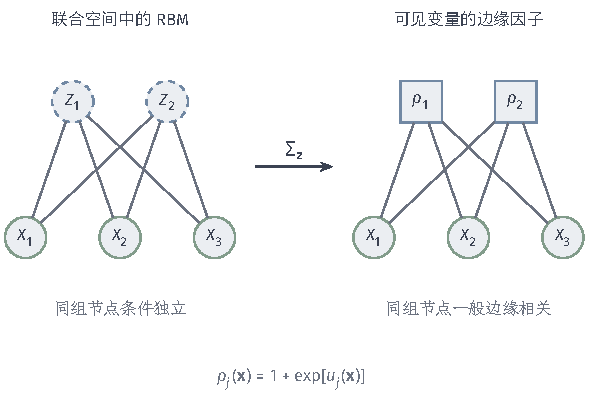
\includegraphics[width=99.653mm]{figures/06-probabilistic-graphical-models/04-models/tikz/pgm-energy-models-rbm/figure.pdf}
  \caption{RBM的条件分解与隐藏消元。左侧仅有跨组边，固定一组时另一组条件独立；右侧把两个隐藏节点消去，两个因子$1+\exp[u_j(\bm{x})]$各涉及三个可见变量。一元可见偏置势在两侧均省略。可见边缘仍可能相关。}
  \label{fig:pgm-energy-models-rbm}
\end{figure}

取两个可见节点和一个隐藏节点，偏置均为零，$W_{1,1}=W_{2,1}=\log2$。可见权重为$e^{-F(\bm{x})}=1+2^{x_1+x_2}$，配置$(0,0),(0,1),(1,0),(1,1)$的权重依次为$2,3,3,5$，总和为$13$。给定$(x_1,x_2)=(1,1)$，隐藏状态为$1$的概率是$4/5$。给定$z=0$时，两可见节点独立、取$1$概率各为$1/2$；给定$z=1$时，该概率各为$2/3$。消去隐藏状态后，$p(X_1=X_2=1)=5/13$与$p(X_1=1)p(X_2=1)=(8/13)^2$相差$1/169$，独立性没有保留。

单个可见配置的自由能求值为$O(d_{\mathrm{v}}m)$，其权重总和$Z_{\bm{\theta}}=\sum_{\bm{x}}e^{-F_{\bm{\theta}}(\bm{x})}$通常仍需指数计算。枚举较小的一组、解析消去另一组虽可减少运算，仍含$2^{\min(d_{\mathrm{v}},m)}$规模。RBM使完整可见配置下的隐藏后验可算，没有普遍消除联合归一化成本。部分可见量未测时，$p(\bm{z}\mid\bm{x}_{\mathrm{obs}})$也未必保有上述独立Bernoulli分解。

这两个块条件可以构成\term{交替Gibbs采样}（alternating Gibbs sampling）：固定一组，独立随机抽取另一组，再交换两组。算法~\ref{alg:pgm-energy-models-rbm-gibbs}传递的是抽到的二值状态；若直接传递概率，所得确定性迭代已不再使用这个Gibbs核。

\begin{algorithm}[RBM的一段交替Gibbs链]
  \label{alg:pgm-energy-models-rbm-gibbs}
  \begin{algorithmic}[1]
    \Require 固定的有限参数$\bm{\theta}$，初始状态$\bm{x}^{(0)}$，步数$k\geq1$
    \Ensure 链状态$\bm{x}^{(1)},\ldots,\bm{x}^{(k)}$
    \For{$t=0,\ldots,k-1$}
      \State 按式~\eqref{eq:pgm-energy-models-rbm-conditionals}独立抽取各$Z_j^{(t+1)}$
      \State 固定$\bm{z}^{(t+1)}$，独立抽取各$X_i^{(t+1)}$
    \EndFor
  \end{algorithmic}
\end{algorithm}

固定有限参数下，每个块条件概率都在$0$与$1$之间，可见状态链因而能到达任意配置，并有自转移。交替Gibbs核保持$p_{\bm{\theta}}(\bm{x})$不变，有限不可约、非周期链的分布遂长期收敛到它；这并未给出小$k$充分混合的保证（参见第~\ref{chap:pgm-sampling}章）。完整一次更新为$O(d_{\mathrm{v}}m)$，强权重形成的近确定条件可能使链长期停留在同一模式。

训练一个权重时，需要提高数据配置的概率，同时扣除模型自身的联合统计。对单条数据$\bm{x}$，潜变量似然梯度在RBM中写为（通用推导参见第~\ref{chap:pgm-parameter-learning}章）
\begin{equation}
  \frac{\partial\log p_{\bm{\theta}}(\bm{x})}
       {\partial W_{i,j}}
    =x_i\,p_{\bm{\theta}}(Z_j=1\mid\bm{x})
      -\mathbb{E}_{p_{\bm{\theta}}}[X_iZ_j].
  \label{eq:pgm-energy-models-rbm-gradient}
\end{equation}
数据项由隐藏条件概率精确取得，模型项则通常需要采样。多条记录对数据项求平均，偏置的梯度对应一阶统计量。RBM简化的是给定数据的后验计算，模型期望仍然存在。重构误差与似然也有不同含义：慢混合的短链容易留在起始数据附近，却可能没有正确分配不同模式的概率质量\scite{pgm-energy-models-hinton2010}

图~\ref{fig:rbm-alternating-sampling-and-gradient}按这一顺序区分概率、抽样状态与训练统计：先固定参数运行交替链、估计模型统计，再用数据统计减模型统计更新参数。

\begin{figure*}[htbp]
  \centering
  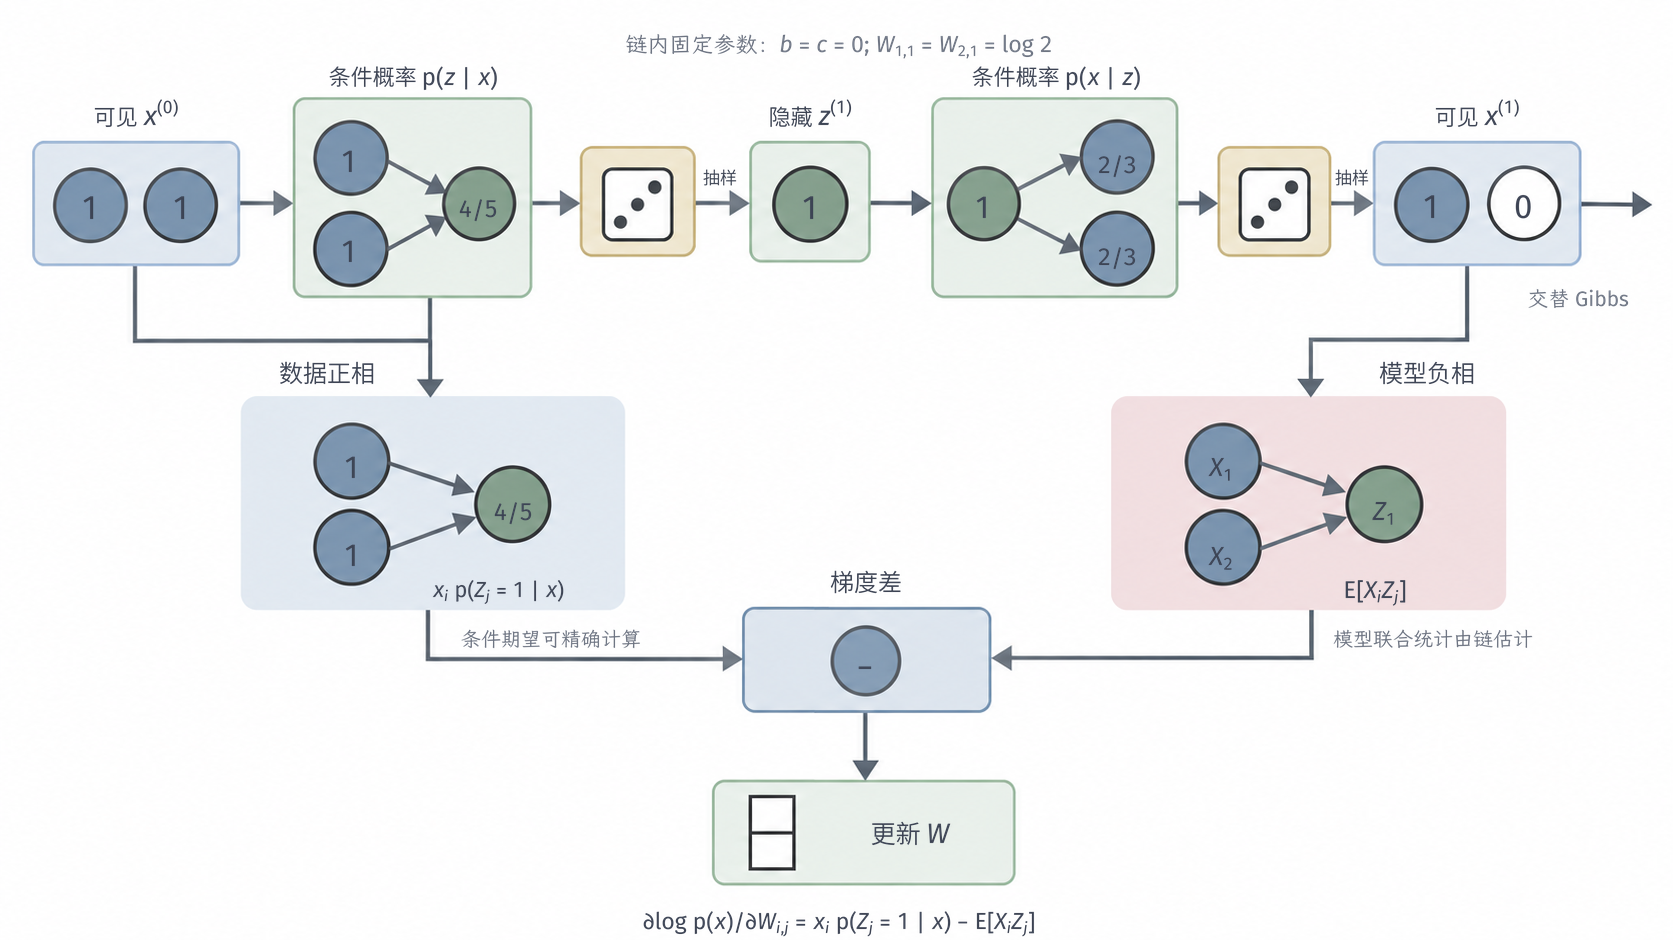
\includegraphics[width=141.647mm]{figures/06-probabilistic-graphical-models/04-models/generated/rbm-alternating-sampling-and-gradient/figure.png}
  \caption{二值RBM中的抽样状态和训练统计。取$b=c=0$、$W_{1,1}=W_{2,1}=\log2$，可见状态$(1,1)$对应隐藏条件概率$4/5$；若抽到$z=1$，可见单元的条件概率各为$2/3$，下一状态可以是$(1,0)$。图中概率与抽样值分别标出。似然梯度以可算的数据统计减去采样估计的模型联合统计，单步重构不能证明混合已完成。}
  \label{fig:rbm-alternating-sampling-and-gradient}
\end{figure*}

\subsection{灵活能量模型}
\label{sec:pgm-energy-models-flexible}

成对二值作用和二次能量限制了相容关系的函数形式。若需要表达更复杂的非线性关系，可以让神经网络为一个配置输出标量能量。\term{神经能量模型}（neural energy-based model）仍按$p_{\bm{\theta}}(\bm{x})\propto e^{-E_{\bm{\theta}}(\bm{x})}$形成分布，改变的是能量函数族。网络的确定性隐藏激活只是计算过程；只有为隐藏量定义了随机分布，才需要把它作为概率潜变量边缘化。

采用$E_{\bm{\theta}}(\bm{x})=\sum_CE_{\bm{\theta},C}(\bm{x}_C)$时，局部网络可以丰富势的形状，同时保留原作用域规定的条件独立性。直接由一个网络读取全部$x_i$而不施加分解，则可能产生全局势；网络内部的计算连线不能代替数据变量的Markov图。函数形式更丰富并不自动降低推断宽度。

连续神经能量能否定义概率，还取决于尾部是否使积分有限。可以在灵活项之外加入二次增长，采用以下充分条件：
\[
  E_{\bm{\theta}}(\bm{x})
    =\frac{\alpha}{2}\lVert\bm{x}\rVert_2^2+r_{\bm{\theta}}(\bm{x}),
  \qquad \alpha>0,\quad r_{\bm{\theta}}(\bm{x})\geq-C,
\]
取有限常数$C$，要求能量可测、在某个正测度集合上有限。上式给出$e^{-E_{\bm{\theta}}(\bm{x})}\leq e^Ce^{-\alpha\lVert\bm{x}\rVert_2^2/2}$，高斯上界保证积分有限，有效支持保证积分为正，合起来得$0<Z_{\bm{\theta}}<\infty$。一般网络不会自动满足这些条件。也可以明确限制到有限体积支持，并保证能量有适当下界。

条件分类得分尚不足以确定输入密度。有限标签上的softmax将$s_k(\bm{x})$转为$p(Y=k\mid\bm{x})$；所有类别得分同时加$c(\bm{x})$，条件概率不变，$\sum_ke^{s_k(\bm{x})}$却改变。因此分类训练不能唯一规定$p(\bm{x})$，单个得分也不能直接解释成$\log p(\bm{x})$。联合能量的支持、归一化对象与训练目标仍需另行给出。

一般神经能量缺少RBM的解析块条件，连续状态可以转用能量对输入的梯度来采样。在无约束$\mathbb{R}^d$上，连续可微能量的一种Langevin离散更新是
\begin{equation}
  \begin{aligned}
    \bm{x}^{(t+1)}
      &=\bm{x}^{(t)}
        -\frac{\varepsilon}{2}
          \nabla_{\bm{x}}E_{\bm{\theta}}(\bm{x}^{(t)})
        +\sqrt{\varepsilon}\,\bm{\xi}^{(t)},\\
    \bm{\xi}^{(t)}&\sim\mathcal{N}(\bm{0},\bm{I}),
       \qquad \varepsilon>0.
  \end{aligned}
  \label{eq:pgm-energy-models-langevin}
\end{equation}
各步独立的高斯噪声使状态在下降方向之外也能探索邻近区域。固定步长、未经Metropolis校正的离散链一般存在偏差，稳定性还依赖梯度条件；有限步运行另有初始化及混合误差。用于估计模型期望的链状态称为负样本。一次能量梯度求值若耗时$C_E$，一条$k$步链的梯度成本为$O(kC_E)$；计算量应包括每步梯度求值，不能仅按一次网络前向传播估计。Du与Mordatch展示了这类连续神经能量的梯度采样实现，其有限步程序本身不构成任意能量下精确采样的保证\scite{pgm-energy-models-du2019}

对比散度从数据配置启动短链，用终点统计替代模型期望；持久链沿用上轮状态，以跟踪缓慢变化的模型。二者近似了取得模型期望的过程，有限步更新未必等于精确似然梯度。神经能量的形状也会受到这种误差影响：负样本若只覆盖局部区域，其他区域的低能量值可能没有受到训练约束。短链终点随参数变化，忽略其分布导数也是对比散度不一般等于某个固定目标精确梯度的原因（参见第~\ref{chap:pgm-parameter-learning}章）。

若希望避免每轮生成模型链，可以用已知噪声密度$p_{\mathrm{N}}$进行噪声对比估计。其分类对数比为$-E_{\bm{\theta}}(\bm{x})+c-\log[\nu p_{\mathrm{N}}(\bm{x})]$，其中$\nu$是噪声与数据的数量比，$c$作为全局对数归一化参数学习。该目标显式使用噪声密度及采样比例，噪声还须覆盖相关支持，故不等于任意的数据分类训练。高维噪声过易区分时，分类信号可能不足以细化数据附近的密度。

光滑连续密度还可以匹配输入对数密度的梯度。由于$\nabla_{\bm{x}}\log p_{\bm{\theta}}=-\nabla_{\bm{x}}E_{\bm{\theta}}$，分数匹配不需要求$Z$的值。相关导数须可积、分部积分的边界项须为零；满足这些条件时，去掉与参数无关的项后，目标为（推导参见式~\eqref{eq:pgm-parameter-learning-score-matching}）
\[
  \mathbb{E}_{p_*}\!\left[
      \frac12\lVert\nabla_{\bm{x}}E_{\bm{\theta}}(\bm{X})\rVert_2^2
      -\Delta_{\bm{x}}E_{\bm{\theta}}(\bm{X})\right],
\]
这里$p_*$为数据分布，$\Delta_{\bm{x}}$求各坐标二阶偏导之和。省去归一化后，成本转为输入导数，尤其是Hessian迹的计算或估计。标准目标针对连续状态；离散状态或受限支持须另行处理，不能省略相应边界项。训练时无需计算$Z$也不表示训练后已经知道它。加噪数据上的分数学习另见第~\ref{chap:pgm-generative}章。

\subsection{高阶与关系联合模型}
\label{sec:pgm-energy-models-higher-relational}

一组传感器恰有一个激活，或设备、连接及报警共同满足某项规则，都是整组状态的约束。\term{高阶势}（higher-order potential）用至少三个变量共同决定权重。对二值组，记激活数$k_C=\sum_{i\in C}\mathbf{1}\{x_i=+1\}$，可以以$g(k_C)$评价计数。取$\lambda>0$、$k_0\in\{0,\ldots,|C|\}$时，$\lambda\mathbf{1}\{k_C\ne k_0\}$惩罚不符目标计数，$\lambda\mathbf{1}\{0<k_C<|C|\}$惩罚组内不一致。

较大的作用域也可能只是低阶项的另一种写法：$(k_C-k_0)^2$展开后只含常数、一元及成对项。要识别不可约高阶作用，可取三个$\{-1,+1\}$变量，令$p(\bm{x})\propto\exp(\lambda x_1x_2x_3)$、$\lambda\ne0$。乘积符号决定偏好，且满足
\[
  \sum_{\bm{x}\in\{-1,+1\}^3}
     x_1x_2x_3\log p(\bm{x})=8\lambda.
\]
在该求和中，归一化常数对应的项为零，三阶项留下八个$\lambda$。若这个正分布可以仅用原三变量的一元与成对势表示，每项对数势都遗漏至少一个变量，先对遗漏变量求和便得零，左侧因此应为零，与$\lambda\ne0$矛盾。这排除了原变量上的成对改写；增加潜变量后则可能采用另一种表示。

高阶势的内部结构决定局部计算量。任意$r$变量二值稠密因子有$2^r$个表项，对一个变量发送消息通常需遍历另$2^{r-1}$种配置。计数势可以先动态规划汇总其余节点恰有$k$个激活的权重。接收节点未激活时，该权重乘$e^{-g(k)}$；接收节点激活时，组内计数增加一，改乘$e^{-g(k+1)}$。分别对$k$求和便得到两种状态的消息，单个输出消息的卷积为$O(r^2)$。这只简化本地因子，未消除其他因子形成的全局环。学习的统计量相应换为计数指示或整体一致性，梯度仍比较经验统计与模型期望。

同一种规则若要用于许多设备，可以将重复因子写成\term{关系模板}（relational template）：规定哪些实体类型及关系参与作用域、哪些实例共享参数。以具体实体替换占位符称为\term{落地}（grounding），得到的还是普通图模型。共享参数减少了参数数量，落地节点和因子仍可能很多，重叠实例也并不独立。

\term{Markov逻辑网络}（Markov logic network, MLN）以逻辑公式组织模板，用成立的落地次数给配置评分。以下限制实体域$D$及谓词集合均有限，并排除产生无限项的函数符号；公式中的自由实体变量遍历域元素。每个落地原子命题是一个Boolean随机变量，配置$\bm{x}$列出全部真值。给模板$r$权重$w_r$、记其落地集合为$\mathcal{I}_r(D)$，联合模型写为
\begin{equation}
  \begin{aligned}
    n_r(\bm{x})
      &=\sum_{g\in\mathcal{I}_r(D)}
           \mathbf{1}\{\text{公式 }r\text{ 在落地 }g\text{ 上为真}\},\\
    E_{\bm{\theta}}(\bm{x})&=-\sum_rw_rn_r(\bm{x}),\\
    p_{\bm{\theta}}(\bm{x})
      &=Z_{\bm{\theta}}^{-1}
          \exp\!\left[\sum_rw_rn_r(\bm{x})\right].
  \end{aligned}
  \label{eq:pgm-energy-models-mln}
\end{equation}
逻辑蕴含说明公式何时成立，不是有向概率边。正权重奖励满足公式的配置；权重有限时，违反公式的实例仍可有非零概率，并非硬性规则。

模板$\operatorname{Fault}(a)\Rightarrow\operatorname{Alarm}(a)$涉及同一设备的故障与报警。若要表达跨设备的相互作用，还可以使用
\[
  \operatorname{Linked}(a,b)\land\operatorname{Fault}(a)
       \ \Rightarrow\ \operatorname{Fault}(b)
\]
将$(a,b)=(u,v)$代入后，连接及两个故障原子共同进入一个因子；连接未观测时，它构成三阶作用。概率图连线说明命题共同参与某个因子，不能直接解释成实体存在物理连接。将连接设为证据会简化因子，所做的是原联合分布的条件化。

逻辑权重与规则概率也需区分。只给一个设备使用首个模板，取$w=\log4$且无其他势，以$F,A$记故障、报警真值。配置$(0,0),(0,1),(1,0),(1,1)$中，三个满足蕴含的权重为$4$，违反配置$(1,0)$的权重为$1$，所以$Z=13$。公式成立概率为$12/13$，条件报警概率$p(A=1\mid F=1)=4/5$，边缘报警概率$p(A=1)=8/13$。三项查询针对不同事件或条件，不能把权重直接当作其中任何一个概率；重叠模板还会使查询依赖周围证据。

学习$w_r$时，似然梯度累加全部落地实例，比较观测的$n_r$与模型期望。完整观测可以使用伪似然；部分命题未观测时，数据统计也需后验推断。消元、近似消息及采样作用于落地后的模型。域大小$N=|D|$、模板有$q$个实体占位符时，实例数可能达$O(N^q)$，精确推断还受落地图宽度约束。模板简短和参数共享并未消除这些成本，MLN的构造及伪似然学习参见原始工作\scite{pgm-energy-models-richardson2006}

硬规则排除违反配置；相互矛盾时可能没有正权配置，即$Z=0$，可行区域分离时单点采样也可能无法穿越。软规则虽避免这种排除，扩大实体域仍会改变落地次数与模板的相对作用，复用原权重未必保持原边缘概率。关系共享规定重复结构及参数合并，不自动保证不同域规模下的概率一致性。

\section{条件能量模型}
\label{sec:pgm-energy-models-conditional-models}

若温度、历史摘要和传感器类型已经给定，检测任务可以只预测异常标签。为这些输入另拟联合分布未必是必要步骤。条件能量将输入作为已知量，专门表达标签之间的相容性；标签配置共同竞争概率质量，仍须处理全局输出归一化。

\subsection{条件随机场的定义}
\label{sec:pgm-energy-models-crf-definition}

固定输入之后，可以用无向图规定标签的条件独立关系。满足这种Markov性质的条件分布称为\term{条件随机场}（conditional random field, CRF），通常通过输入相关的团势构造：
\begin{equation}
  \begin{aligned}
    p_{\bm{\theta}}(\bm{y}\mid\bm{x})
      &=\frac{1}{Z_{\bm{\theta}}(\bm{x})}
          \prod_{C\in\mathcal{C}}
             \psi_{\bm{\theta},C}(\bm{y}_C,\bm{x}),\\
    E_{\bm{\theta}}(\bm{y},\bm{x})
      &=-\sum_{C\in\mathcal{C}}
             \log\psi_{\bm{\theta},C}(\bm{y}_C,\bm{x}).
  \end{aligned}
  \label{eq:pgm-energy-models-crf-factors}
\end{equation}
该图只以输出变量为节点。固定输入，若$S$分离$A$、$B$，则$\bm{Y}_A\perp\bm{Y}_B\mid(\bm{Y}_S,\bm{x})$。完整输入可以被多个势或序列编码器读取；标签作用域由一个势同时涉及哪些未知标签决定，不能从输入编码器的连线推定。

既有联合Markov模型$p(\bm{x},\bm{y})$条件化后也能给出CRF形式，直接条件拟合则只学习$p(\bm{y}\mid\bm{x})$，不同时约束$p(\bm{x})$。反向组成联合分布时，必须为CRF另选输入分布。输入缺失需要边缘化时，同样缺少其分布，单凭条件标签模型无法完成这项查询。

常用的线性形式为$\log\psi_{\bm{\theta},C}=\bm{\theta}^\top\bm{f}_C(\bm{x},\bm{y}_C)$，各作用域可以共享参数。给定完整标签记录$\{(\bm{x}_r,\bm{y}_r)\}_{r=1}^n$，比较观测特征得分与该输入下全部标签的权重总量，条件对数似然为
\begin{equation}
  \ell_{\mathrm{cond}}(\bm{\theta})
    =\sum_{r=1}^n
       \left[
        \sum_C\bm{\theta}^\top
                    \bm{f}_C(\bm{x}_r,\bm{y}_{r,C})
        -\log Z_{\bm{\theta}}(\bm{x}_r)
       \right].
  \label{eq:pgm-energy-models-crf-likelihood}
\end{equation}
不同输入一般给出不同配分函数，梯度要逐条计算条件标签边缘及期望特征，推断因而反复参与训练。固定特征、完整标签的线性参数化使对数似然为凹函数，有限最优解仍取决于可分离性与正则化；可训练神经特征或未观测标签的边缘化则不保留一般凹性结论（梯度推导参见第~\ref{sec:pgm-parameter-learning-conditional}节）。以时间或序列位置重复输出关系时，可以进一步得到链与片段模型，其详细计算见第~\ref{chap:pgm-dynamic-undirected}章。CRF的完整表述见Sutton与McCallum\scite{pgm-energy-models-sutton2012}

\subsection{一般图与关系条件随机场}
\label{sec:pgm-energy-models-general-relational}

二维位置或相互连接的设备，可能需要保留链之外的标签关系。一般图CRF继续用式~\eqref{eq:pgm-energy-models-crf-factors}，改由输出关系规定作用域；关系CRF将它们写成模板。设备属性、已知连接及图结构属于输入，待预测标签才是未知变量。

例如，每个设备有标签$Y_i$，属性形成一元势，每条已知连接复用同一相邻标签势。若输入$\bm{x}$进一步确定模板$r$的实例集$\mathcal{I}_r(\bm{x})$，各实例的得分相加为
\begin{equation}
  E_{\bm{\theta}}(\bm{y},\bm{x})
   =-\sum_r\sum_{g\in\mathcal{I}_r(\bm{x})}
        \bm{\theta}_r^\top
             \bm{f}_r(\bm{x}_g,\bm{y}_g).
  \label{eq:pgm-energy-models-relational-crf}
\end{equation}
实例$g$选定具体实体及关系作用域，$\bm{x}_g$收集已知特征，$\bm{y}_g$包含参与的未知标签。共享参数$\bm{\theta}_r$接收各实例的学习统计；实例可能重叠，不能因此当作独立记录。Taskar等人的关系Markov网络给出了这种条件分布与集体分类的代表构造\scite{pgm-energy-models-taskar2002}

给定关系输入后，标签图仍可能成环，例如设备连接本身形成闭环。团树可以精确汇总它的概率（参见第~\ref{chap:pgm-junction-tree}章），成本取决于消元后的作用域。标签数为$K$、所用消元序诱导宽度为$w$时，主要计算一般含$K^{w+1}$规模。简单环宽度仍小，不必一律近似；密集关系或大型高阶作用域则可能超出可用资源。

宽图难以精确处理时，可近似边缘或最优配置。平均场、环置信传播及采样用于概率与期望，最大化松弛、图割或整数优化针对最优配置（参见第~\ref{chap:pgm-variational}、\ref{chap:pgm-sampling}章）。后一个问题的解不会自动给出前一个问题的概率。环消息可能不收敛，收敛值也未必是精确边缘；据此训练时，须说明使用了近似梯度或配分函数。

关系势错误也会沿集体推断传播。若所有连接都奖励同标签，而实际常连接不同故障类型，多个节点可能共同偏移；高连接度还使一个位置重复参与许多势。需要检查特征与共享方式，延长消息迭代无法修复这种错设。连接仅作为已知输入时，其生成分布仍未定义，标签推断不能自行扩展为未知连接生成。

评价须说明预测发生在同一张关系图还是新图。同图中已标注、未标注节点的划分属于传导任务，与预测全新独立图不同；测试标签不得借邻域特征进入训练。部分训练标签未观测时，条件似然分子也要边缘化它们，训练增加后验推断并通常失去凹性。共享关系模式可以合并信息，相关性、划分泄漏及推断误差仍要分别控制。

\section{模型比较}
\label{sec:pgm-energy-models-comparison}

模型的区别可以按归一化变量、可见信息及可利用运算逐项比较。表~\ref{tab:pgm-energy-models-comparison}汇总代表设定，所列属性允许组合；例如采用神经高阶势的关系CRF，仍按给定输入的标签空间归一化。这些名称不是互斥类别。

\begin{table*}[htbp]
  \centering
  \small
  \begin{tabularx}{\linewidth}{p{27mm}p{19mm}p{24mm}p{24mm}X}
    \toprule
    代表设定 & 归一化对象 & 变量与潜变量 & 势的作用域 & 可计算性与主要限制\\
    \midrule
    Ising／Potts & 全部状态 & 离散；此处全观测 & 一元、成对 & 树上精确；一般图的全局求和与强耦合采样可能昂贵\\
    高斯MRF & 全部状态 & 连续；此处全观测 & 二次能量 & 正定精度下可解析归一化；矩阵填充与单峰限制\\
    BM／RBM & 可见与隐藏状态 & 二值；含潜变量 & 联合空间成对 & RBM的块条件与自由能可算，联合配分函数一般仍难\\
    神经联合能量 & 全部状态 & 可离散或连续；潜变量可选 & 局部或全局 & 网络求值不等于归一化；尾部、采样和学习偏差均需控制\\
    MLN & 落地命题配置 & Boolean；可有未观测命题 & 模板决定阶数 & 参数共享不消除落地数量及推断宽度的增长\\
    一般图关系CRF & 给定关系输入的标签 & 此处离散；标签可缺失 & 成对或高阶 & 低宽度可精确；宽图依赖近似推断且须重复用于学习\\
    \bottomrule
  \end{tabularx}
  \caption{本章代表模型的归一化与计算条件。潜变量、势阶数和参数化允许组合，条件模型也可定义连续输出；表中只列本章展开的设定。}
  \label{tab:pgm-energy-models-comparison}
\end{table*}

先按查询选择联合或条件对象。若查询涉及输入的生成或概率补全，还需为输入提供概率模型；始终给定输入而只预测标签时，可以直接学习条件分布。输出依然全局归一化，复杂标签图可能仍难以求和，且不同训练输入各有$Z_{\bm{\theta}}(\bm{x})$。

表达能力要同时看势的函数形式和未知变量作用域。GMRF能借二次结构处理环，却仅表示单峰高斯；RBM的成对联合势可诱导高阶边缘，归一化仍可能昂贵。计数高阶势能用卷积，任意高阶表却需指数存储。局部神经势丰富函数形状并保留原图，全局网络则可能失去稀疏分解，不能只按“成对”或“神经”判断可表达范围与代价。

收敛性分析要区分优化目标与计算该目标的误差。完整离散模型需要模型期望，BM还需数据隐藏后验，RBM只简化后者；神经能量通常依靠负样本或输入导数。线性固定特征CRF有凹似然，但期望是否能精确计算还取决于输出图；训练需反复推断；神经参数或隐藏标签不保留一般凹性。应检查有限最优解、优化停止与近似误差，短链重构或单个训练损失不足以说明收敛。

泛化性需要在未参与拟合和调参的数据上评价，并固定预测单位。条件模型可比较同一留出集上按记录平均的负对数似然，值越小越好；单点标签错误与整组标签错误评价不同输出单位，不能互换。关系模型还要区分同图传导与新图预测。联合模型若用留出似然评价，须取得可比较的配分函数估计并报告其误差；训练目标下降本身不保证这些预测指标改善。

\section{本章小结}
\label{sec:pgm-energy-models-summary}

局部相容权重经过共同归一化，才能形成整组状态的概率；能量是权重的负对数写法，添加常数不改分布。三位置联合例子的权重总和为$32$，展示了局部耦合怎样改变整组状态的概率。固定输入后也可以改变标签势，再对输出单独归一化；输入本身无需生成分布。

联合与条件划分归一化对象，其他属性可在其内部组合。潜变量使简单联合作用产生复杂边缘，RBM的二部限制使隐藏后验与自由能可算，联合配分函数仍是训练难点。高阶势及关系模板表达整体约束，也增加作用域、落地规模和可行性要求；神经能量需另查积分尾部及近似学习误差。

固定输入并不意味着标签独立。一般标签图的查询受消元宽度限制；若局部关系沿序列重复，则可利用时间接口组织消息，详见第~\ref{chap:pgm-dynamic-undirected}章。回答开篇问题时，先决定是否需要输入的生成分布，再按所需相互作用选择局部结构，最后确认归一化、推断与学习的成本。表达能力、求解保证和未见数据的预测评价要分别核对。

序列也可以采用有向生成模型：先规定潜状态演化，再为测量定义发射分布，链上的求和与最大化仍可复用（参见第~\ref{chap:pgm-dynamic}章）。这样的观测模型为未来测量的概率预测提供依据；本章固定输入的标签CRF则只规定标签条件分布，未给输入读数建立生成机制。

\paragraph{扩展阅读}
Bishop的PRML和Murphy的教材可继续用于学习能量分布及采样训练。建议分别追踪三个计算对象：配置得分、归一化概率、梯度中的模型期望，并核对何种结构使每项可算；得分容易求值不代表概率和期望也容易求值\scite{bishop2006,pgm-murphy2012}

\chapter{动态有向模型}
\label{chap:pgm-dynamic}

前两章的模型都把每条记录看作一张静态“快照”，记录之间没有先后之分。但设备监测、语音、定位、金融等数据本质上是\emph{随时间展开的序列}：此刻的状态由上一刻演化而来，此刻的传感器读数又只是这个内部状态的一个带噪测量。处理这类数据会遇到两个静态模型里没有的核心问题。第一，\emph{信息要沿时间传递}：判断当前状态时，怎样把整段历史的证据压缩成一个可以递推的量，而不必每来一个新观测就重新处理全部历史？第二，\emph{要把“状态如何演化”和“观测如何由状态产生”这两件事分开}：同一个内部状态可能产生很不相同的读数，而后来的读数还可能反过来修正我们对过去状态的判断。本章研究的动态有向模型，就是用一条有向的状态链把这两个机制分别表示出来，让历史判断能够与新证据\emph{逐步}结合。

学习这类模型还有一个便利：只要把“对未来有用的信息”全部集中到当前状态里，从时刻$t$到$t+1$的更新在\emph{每一步都形式相同}，于是推断变成一条只需维护一个固定大小消息的递推，计算量随序列长度线性增长，而不会随历史长度膨胀。本章的一条主线就是：这个跨时刻要传递的消息包含什么、需要保留多少历史，以及在离散状态和连续状态、线性和非线性等不同设定下，这条递推何时能\emph{精确}计算、何时必须近似。

一台设备连续两次报警，可能意味着故障正在持续，也可能来自传感器误报。前一次状态判断影响我们怎样理解下一次报警；后来的读数又可能改变我们对故障起点的判断。动态有向模型把设备状态的演化与传感器产生读数的机制分别表示，使历史判断可以与新证据逐步结合。本章研究这种递推怎样保存不确定性，以及它需要保留多少历史信息。

按时间组织有向分解后，递推预测只需把过去对未来有用的信息传到下一时刻。消元和消息传递正是完成这一压缩的工具（参考第~\ref{chap:pgm-directed}、\ref{chap:pgm-elimination}、\ref{chap:pgm-junction-tree}章）。本章先确定跨时刻传递的变量，再讨论有限概率表和高斯参数何时能精确保存这些信息。对于隐藏状态，推断还会提供后验统计量，让转移和观测参数可以从序列中学习。

这里的时间表示系统的采样时刻，或任务中有明确前后关系的序列位置。其他序列模型可能把不同对象放在时间轴上：序列条件随机场描述给定观测后的标签分布，适合条件预测（第~\ref{chap:pgm-dynamic-undirected}章）；扩散模型利用人为设定的噪声过程构造生成分布，其步数记录噪声过程的进展（第~\ref{chap:pgm-generative}章）。本章则围绕系统状态怎样演化、观测怎样反映状态展开。

\section{序列状态的建模与学习问题}
\label{sec:pgm-dynamic-common}

本节建立全章通用的序列建模语言：用一张小模板图沿时间复制出整条序列，把变量组织成隐藏状态和观测，并说明由此产生的学习问题。对设备而言，状态既可能是正常、异常这样的离散工况，也可能是连续温度，或由运行模式和温度共同组成。后续先给出共用的序列结构与学习问题，再分别讨论离散、连续和混合状态。这个划分依据当前模型采用的状态表示；把离散历史并入一个大状态，或给连续量离散化，都会改变表示及计算代价，并不产生彼此绝对隔离的模型类别。

\subsection{时间模板、潜状态与序列联合分布}
\label{sec:pgm-dynamic-template}

在绝大多数动态系统里，每个时刻遵循的局部规律是\emph{相同}的——同一台设备的物理规律不会每过一秒就换一套。因此与其为$T$个时刻各画一张图、各设一组参数，不如只画一张描述“一个时刻内部、以及相邻时刻之间如何相连”的\emph{模板}，再让它沿时间轴重复复制。设备在不同采样时刻往往遵循相同的依赖结构。把当前时刻内部的依赖和相邻时刻之间的依赖画成一个模板，再沿时间重复展开，就得到\term{动态有向图模型}（dynamic Bayesian network, DBN）。这一表示框架允许不同的状态空间与局部分布；隐马尔可夫模型和状态空间模型都可以借它组织。

把第$t$个时刻的变量放在同一个\term{时间切片}（time slice）内，记为随机向量$\bm{Y}_t=(Y_{t,1},\ldots,Y_{t,d})^\top$。其中$d$个变量可同时包含观测量和隐藏量。先考虑只连接相邻切片的模型，跨切片的边从$t-1$指向$t$。用$\operatorname{pa}^{-}(i)$记录节点$i$在上一切片的父节点索引，用$\operatorname{pa}^{0}(i)$记录当前切片的父节点索引。有向分解于是给出转移模板
\begin{equation}
  p(\bm{y}_t\mid\bm{y}_{t-1})
  =\prod_{i=1}^{d}
    p\bigl(y_{t,i}\mid
      \bm{y}_{t-1,\operatorname{pa}^{-}(i)},
      \bm{y}_{t,\operatorname{pa}^{0}(i)}\bigr).
  \label{eq:pgm-dynamic-two-slice}
\end{equation}
要求切片内部无环后，可以先按时间、再按切片内的拓扑序排列节点。这个顺序使任意有限长度$T$的展开都保持有向无环结构。序列的起点由初始分布$p(\bm{y}_1)$给定，后续切片再按转移模板生成。式~\eqref{eq:pgm-dynamic-two-slice}这段可重复的相邻切片结构称为\term{两切片动态有向图模型}（two-slice temporal Bayesian network, 2TBN）。

模板里可以放很多变量，但为了让递推清晰，最常用的组织是把变量分成两类：一类是真正\emph{驱动系统演化、并概括了对未来全部影响}的内部状态（它通常看不到），另一类是这个状态产生的、我们能读到的传感器观测。这样安排是为了让“预测未来”只需盯住状态、而不必带着全部历史观测走。一种常用组织方式把影响未来的内部信息集中到潜状态$\bm{z}_t$，把传感器读数记为观测$\bm{x}_t$。状态可以是物理量，也可以是模型为预测而构造的变量。假设给定$\bm{z}_{t-1}$后，$\bm{z}_t$与更早状态条件独立（即下一时刻只依赖当前状态、不需要更早历史）；给定完整状态序列后，各时刻观测条件独立，且$\bm{x}_t$由$\bm{z}_t$产生。这两个局部机制——一个\emph{转移模型}描述状态怎样随时间变化，一个\emph{观测模型}描述状态怎样产生读数——组成\term{状态空间模型}（state space model, SSM）：
\begin{equation}
  \begin{aligned}
    p(\bm{z}_{1:T},\bm{x}_{1:T})
      &=p(\bm{z}_1)p(\bm{x}_1\mid\bm{z}_1)\\
      &\quad{}\times\prod_{t=2}^{T}
        p(\bm{z}_t\mid\bm{z}_{t-1})
        p(\bm{x}_t\mid\bm{z}_t).
  \end{aligned}
  \label{eq:pgm-dynamic-state-space}
\end{equation}
式~\eqref{eq:pgm-dynamic-state-space}把联合分布拆成初始、转移和观测三类因子，也为粒子滤波提供起点（第~\ref{sec:pgm-sampling-smc}节）。其中$\bm{z}_t$是潜状态，$\bm{x}_t$是观测；下文讨论这类分解何时能精确递推，并用于参数学习。记号$p$兼指概率质量函数和相对于相应测度的密度，离散状态的积分按求和理解。小写粗体表示向量；标量离散模型使用随机变量$Z_t,X_t$及取值$z_t,x_t$。图~\ref{fig:pgm-dynamic-template}展开了三个时刻，每个潜状态既产生当前观测，也传递未来所需的信息。允许观测间连边或更复杂切片内依赖的DBN则超出了这个状态空间特例。

\begin{figure}[htbp]
  \centering
  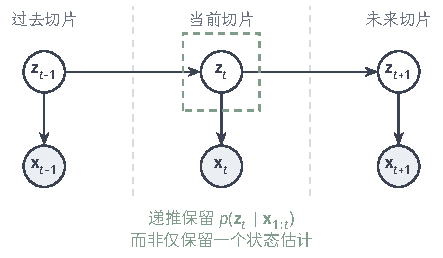
\includegraphics[width=74.997mm]{figures/06-probabilistic-graphical-models/04-models/tikz/pgm-dynamic-template/figure.pdf}
  \caption{状态空间模型在三个时刻的展开。空心节点为潜状态，填色节点为观测，竖直虚线分隔时间切片。当前潜状态的后验汇总过去证据，用于下一步预测；箭头表示生成依赖，平滑计算则沿状态链反向传递未来证据。}
  \label{fig:pgm-dynamic-template}
\end{figure}

有了联合分解，还需要说明哪些量从数据中估计。设训练集包含$N$条独立收集的序列$\bm x^{(n)}_{1:T_n}$，$\bm\theta$汇总初始、转移和观测分布中的待估参数。观测没有给出状态路径，因而每条观测序列的概率需要累加所有可能状态的贡献。参数学习的共同目标是
\begin{equation}
  \widehat{\bm\theta}\in\argmax_{\bm\theta\in\Theta}
  \ell(\bm\theta),\qquad
  \ell(\bm\theta)=\sum_{n=1}^N
  \log\int p_{\bm\theta}(\bm z_{1:T_n},\bm x^{(n)}_{1:T_n})
       \,\mathrm d\bm z_{1:T_n}.
  \label{eq:pgm-dynamic-observed-objective}
\end{equation}
其中$\Theta$要求各局部分布合法，离散状态把积分改成求和。正则或先验会改变这个目标，不能只在更新时任意加入修正。模型拟合后，状态推断是在固定参数下重新计算后验；它与对$\bm\theta$的优化是两个不同问题。

\subsection{状态记忆与跨时刻依赖}
\label{sec:pgm-dynamic-memory}

动态模型最关键的一个简化假设是：为了预测下一步，\emph{无需更早的历史}，知道当前状态就够了——更早的信息都已被当前状态“吸收”。这有点像下棋时只需知道当前棋局，而不必记住此前每一步怎么走的。递推需要保留多少历史，取决于状态怎样选择。\term{Markov假设}（Markov assumption）要求给定当前状态后，预测下一状态所需的信息已经齐备。对于$r$阶依赖$p(\bm{z}_t\mid\bm{z}_{t-r:t-1})$，可以把最近$r$个状态拼接成一个扩充状态，从而改写成一阶模型，代价是扩大状态空间。观测只间接反映内部状态，因此观测历史仍可能持续改变当前状态的后验，即使潜状态满足一阶Markov性。

设备每次按相同规则升温，温度分布仍会从冷启动逐渐向高温移动。这里保持的是局部机制：\term{时间齐次性}（time homogeneity）要求转移核不随$t$改变；\term{参数共享}（parameter sharing）表示不同位置复用同一组转移或观测参数。共享参数的条件分布若还依赖时间或已知外部输入，取值仍可随时刻变化。\term{严格平稳性}（strict stationarity）约束的则是整个过程，要求任意有限组时刻的联合分布在整体平移后保持不变。齐次Markov链从平稳分布初始化时，才得到这样的平稳过程。

将过去变量消去后，需要把哪些信息留给未来？所有跨越时间分界的依赖经过的变量集合称为\term{时间接口}（temporal interface）。一阶状态空间模型只需保留$\bm{z}_t$的后验，因为给定这个状态，过去与未来被分开。一般DBN可以保留当前切片中有下一切片子节点的变量及其联合分布。过去证据可能让这些变量相关，联合分布因此包含单独边缘没有保存的信息。计算代价取决于离散接口的联合配置数，或连续后验的表示复杂度，这也是消元中诱导宽度的重要来源（第~\ref{chap:pgm-elimination}章）。Koller和Friedman详细讨论了图模板、时间接口与精确推断的关系\scite{pgm-koller2009}。

\subsection{预测、状态重建与参数学习的接口}
\label{sec:pgm-dynamic-queries}

在进入具体模型前，先把对一条时间序列能提的几类问题区分清楚，因为它们读取证据的时间范围不同、对应不同算法：是预测\emph{未来}、估计\emph{此刻}，还是事后追溯\emph{过去}。设备监测提出三类查询。\term{预测}（prediction）给出$p(\bm{z}_{t+h}\mid\bm{x}_{1:t})$或$p(\bm{x}_{t+h}\mid\bm{x}_{1:t})$，其中$h\geq1$，用于判断未来状态或读数——此刻做决策时只允许用到目前为止的数据。\term{滤波}（filtering）给出$p(\bm{z}_t\mid\bm{x}_{1:t})$，用于\emph{在线}地、收到一个新读数就更新一次当前状态判断（像实时跟踪）。\term{平滑}（smoothing）给出$p(\bm{z}_t\mid\bm{x}_{1:T})$，其中$t<T$，用于\emph{事后}结合“未来才拿到的证据”重建过去（像检修时回看整段记录），因此通常比在线滤波判断得更准。固定间隔平滑读取长度为$T$的整段数据；固定滞后平滑只等待预定步数的未来观测，适合允许延迟的状态判断。

重建整段工况还可能需要\term{最可能状态序列}（most probable state sequence），即让$p(\bm{z}_{1:T}\mid\bm{x}_{1:T})$达到最大的整条路径。对全部潜状态求最大值得到MPE查询；保留部分状态求最大值、其余状态求和或积分，则得到边缘MAP（第~\ref{chap:pgm-elimination}章）。逐时刻取平滑边缘的最大项，对应按各位置误判数评价的决策；整条路径优化评价的是联合概率，两种目标可能选择不同结果。连续状态的路径最优以所选坐标和基准测度下的后验密度为准。

预测和滤波可以从当前后验逐步计算，平滑则在此基础上加入未来证据。记上一步滤波分布为$f_{t-1}(\bm{z}_{t-1})=p(\bm{z}_{t-1}\mid\bm{x}_{1:t-1})$。将它与转移分布结合并消去旧状态，得到当前预测；再乘当前观测似然并归一化，得到
\begin{equation}
  \begin{aligned}
    f_t^{-}(\bm{z}_t)
      &=\int p(\bm{z}_t\mid\bm{z}_{t-1})
        f_{t-1}(\bm{z}_{t-1})\,\mathrm{d}\bm{z}_{t-1},\\
    c_t
      &=\int p(\bm{x}_t\mid\bm{z}_t)
        f_t^{-}(\bm{z}_t)\,\mathrm{d}\bm{z}_t,\\
    f_t(\bm{z}_t)
      &=\frac{p(\bm{x}_t\mid\bm{z}_t)
        f_t^{-}(\bm{z}_t)}{c_t}.
  \end{aligned}
  \label{eq:pgm-dynamic-bayes-filter}
\end{equation}
第一次预测取$f_1^{-}=p(\bm{z}_1)$；每个归一化量$c_t$需有限且为正。它同时等于$c_t=p(\bm{x}_t\mid\bm{x}_{1:t-1})$，所以$\log p(\bm{x}_{1:T})=\sum_{t=1}^{T}\log c_t$给出整段观测的对数似然。一次递推因而既更新状态判断，也累计训练和模型比较需要的分数。有限状态与线性高斯模型的优势在于，这些积分或求和可以精确计算，结果仍有固定大小的表示。

\section{离散状态序列的建模与学习}
\label{sec:pgm-dynamic-discrete}

从离散状态入手最简单：状态只取有限个类别（正常/异常/故障前兆），于是“转移模型”就是一张概率表，所有求和都可以在这些有限状态上精确完成。先从最容易的情形讲起——状态能被直接看到（巡检记录了工况），这时只要数一数状态之间转移的次数就能估计转移表；再进入更常见也更难的情形——状态看不到、只有带噪观测，这时要对所有可能的隐藏路径求和。离散工况只取有限类别；其演化可以用转移概率表表示。若巡检直接记录工况，数据给出真实转移次数；若只有传感器读数，就要汇总可能的隐藏路径，再以期望次数学习。下面在这个共同问题下分别处理可见状态和隐藏状态。

\subsection{可见状态：转移结构与计数学习}
\label{sec:pgm-dynamic-visible}

如果每次巡检都能可靠记录设备的正常或异常状态，训练序列就直接给出了状态转移。用$Z_t\in\{1,\ldots,K\}$表示有限状态，$\pi_i=p(Z_1=i)$表示初始概率。齐次转移矩阵$\bm{A}\in\mathbb{R}^{K\times K}$的元素为
\[
  a_{i,j}=p(Z_t=j\mid Z_{t-1}=i),\qquad
  a_{i,j}\geq0,\quad \sum_{j=1}^{K}a_{i,j}=1.
\]
矩阵每一行列出从一个当前状态到各下一状态的概率，非负且总和为一。本节考虑有限状态、离散时间和齐次转移，初始概率$\bm\pi$按列向量记录（Markov关系参见\BookChapterRef{chap:random-variables}{卷2《数学准备：概率、因果与决策》的“随机变量”章}）。

初始概率和转移表共同定义整条可见路径的概率。训练记录为$z^{(n)}_{1:T_n}$时，本模型的结构和学习目标可明确写为
\begin{equation}
  \begin{aligned}
    p_{\bm\theta}(z_{1:T})&=\pi_{z_1}
       \prod_{t=2}^{T}a_{z_{t-1},z_t},\\
    \ell_{\mathrm{MC}}(\bm\theta)
       &=\sum_{n=1}^{N}\log\pi_{z^{(n)}_1}
           +\sum_{i,j}n_{i,j}\log a_{i,j}.
  \end{aligned}
  \label{eq:pgm-dynamic-visible-objective}
\end{equation}
这里$n_{i,j}$是所有记录内$i\to j$的总次数，$\bm\theta=(\bm\pi,\bm A)$满足概率非负和归一化约束。最大化该式就是让数据实际出现的起点与转移获得较大概率；各行归一化又防止所有转移概率同时增大。先看给定参数怎样预测，再利用同一分解求参数。

把当前状态分布记为概率列向量$\bm{q}_t$。对随机状态$Z_t$求和，下一步分布满足$\bm{q}_{t+1}=\bm{A}^{\top}\bm{q}_t$。重复这一计算便得到
\begin{equation}
  \bm{q}_{t+h}=(\bm{A}^{\top})^h\bm{q}_t,\qquad
  p(Z_{t+h}=j\mid Z_t=i)=(\bm{A}^h)_{i,j}.
  \label{eq:pgm-dynamic-markov-prediction}
\end{equation}
两步转移中的$\sum_k a_{i,k}a_{k,j}$累加了经过各个中间状态的路径概率。继续累加中间状态，就得到$h$步矩阵幂；转置来自概率列向量与按行定义的转移矩阵之间的约定。

\begin{example}[两状态设备的多步预测]
  \label{ex:pgm-dynamic-markov}
  为单独展示多步预测，设状态$1$为正常、状态$2$为异常，采用下面的人工参数。它与四节点报警模型及例~\ref{ex:pgm-sampling-filter}分别设定，后面的发射概率也将另给：
  \[
    \bm{\pi}=\begin{pmatrix}0.8\\0.2\end{pmatrix},\qquad
    \bm{A}=
    \begin{pmatrix}0.9&0.1\\0.2&0.8\end{pmatrix}.
  \]
  从确定正常的状态出发，下一步异常概率为$0.1$；两步后需要累加先正常后异常和先异常后异常两条路径，得到$0.9\times0.1+0.1\times0.8=0.17$。当前异常概率为$u_t$时，递推为
  \[
    u_{t+1}=0.1(1-u_t)+0.8u_t=0.1+0.7u_t.
  \]
  解得$u_{t+h}=1/3+0.7^h(u_t-1/3)$。初始偏差随预测步数按几何因子衰减，异常概率趋向$1/3$；这个极限由正常进入异常和异常退出两种转移共同决定。
\end{example}

例~\ref{ex:pgm-dynamic-markov}的极限是平稳分布$(2/3,1/3)^\top$，满足$\bm A^\top\bm\pi_\star=\bm\pi_\star$。平稳分布给出转移后保持不变的分布；从任意初态是否趋向它，还取决于链的长期行为条件。时间平均又涉及沿同一条路径累积的观测量，与这里的单时刻分布极限不同。下面转向如何从数据估计转移概率，以及状态隐藏时怎样推断。

可见状态的参数学习可以直接使用转移计数。令$n_{i,j}$为训练序列中$i\to j$的次数，转移对数似然为$\sum_{i,j}n_{i,j}\log a_{i,j}$。在各行总和为$1$的约束下最大化，得到$\widehat a_{i,j}=n_{i,j}/\sum_k n_{i,k}$。从未访问的行会出现$0/0$，意味着数据没有给出该行的信息，可用先验或保留旧值处理。多条独立序列分别计数后汇总，序列之间的接缝不计作转移；初始分布则只统计各序列首状态。

具体地，初始更新为$\widehat\pi_i=N^{-1}\sum_n\mathbf1\{z^{(n)}_1=i\}$。对转移表第$i$行加入乘子$\lambda_i$；正计数项的内点驻点条件为$n_{i,j}/a_{i,j}=\lambda_i$；对$j$求和并使用行和为$1$，得到$\lambda_i=\sum_jn_{i,j}$，因而产生上述计数比例，零计数项可取边界值$0$。没有隐藏变量时，这一步直接求解约束似然，无需反复运行EM。

\subsection{隐藏离散状态的组织与估计}
\label{sec:pgm-dynamic-hidden-discrete}

读数与工况并非一一对应时，我们需要同时表示工况怎样变化，以及每种工况怎样产生读数。先建立逐时刻隐藏状态模型，再分别改变它保存的历史、停留时长和内部组成。这三种变化可以组合，但每次变化都要重新确定求和的路径与学习所需统计量。

\subsubsection{HMM：逐时刻隐藏工况的学习与推断}
\label{sec:pgm-dynamic-hmm-model}

现实中真正能直接读到内部“健康工况”的情形很少，我们拿到的只是报警、温度等间接读数，而且同一个工况可能产生多种读数、同一种读数也可能来自不同工况。要描述这样的数据，需要\emph{两层}：底层是一条隐藏工况按转移表演化的Markov链，上层是“在每种工况下，读数服从什么分布”的观测机制；这就是隐马尔可夫模型——它相当于把第11章的静态混合模型加上时间轴，让前一时刻的成分影响下一时刻的成分，从而能刻画“故障会持续”而不是每刻独立乱跳。设备内部的健康状态通常隐藏在报警、温度等读数之后。用一个有限状态链描述内部演化，再给每个状态指定产生读数的分布，就得到\term{隐马尔可夫模型}（hidden Markov model, HMM）。其中的\term{发射分布}（emission distribution，这是观测模型在离散状态下的叫法，“发射”即隐藏状态把观测“发”出来）描述给定状态后的观测，记$b_j(x)=p(x\mid Z_t=j)$为它在$x$处的概率质量或密度。联合分布为
\begin{equation}
  p(z_{1:T},x_{1:T})
    =\pi_{z_1}b_{z_1}(x_1)
      \prod_{t=2}^{T}a_{z_{t-1},z_t}b_{z_t}(x_t).
  \label{eq:pgm-dynamic-hmm}
\end{equation}
HMM的隐藏状态取离散值，观测则可以是Bernoulli报警，也可以是服从状态相关高斯密度的温度。与独立混合模型相比，它用转移分布连接相邻潜类别，使前一时刻的工况影响下一时刻的成分选择（第~\ref{chap:pgm-static-directed}章）。

模型参数是$\bm\theta=(\bm\pi,\bm A,\{\bm\vartheta_j\}_{j=1}^K)$，其中$\bm\vartheta_j$控制第$j$个发射分布。训练读数仍只告诉我们$x$，不能把某条猜测的状态路径当成观测。需要最大化的目标为
\begin{equation}
  \ell_{\mathrm{HMM}}(\bm\theta)
   =\sum_{n=1}^{N}\log\sum_{z_{1:T_n}}
       \pi_{z_1}b_{z_1}(x^{(n)}_1)
       \prod_{t=2}^{T_n}a_{z_{t-1},z_t}b_{z_t}(x^{(n)}_t).
  \label{eq:pgm-dynamic-hmm-objective}
\end{equation}
求和使每条可能工况路径都按其概率贡献观测似然。后面的前向递推计算这个目标，前向--后向递推提供学习所需的期望计数，最优路径算法则只回答路径决策，三者不能互相替代。

静态混合与HMM之间还存在精确的特例关系。若所有转移行都等于同一成分比例，即$a_{i,j}=\pi_j$，起点也服从$\bm\pi$，且各时刻共享相同发射分布，则潜状态独立同分布，路径求和可以逐时刻分开，得到$\prod_t\sum_j\pi_jb_j(x_t)$。这才退回独立混合观测；仅仅让转移表对角元素较小，并不消除状态之间的依赖。

计算观测序列似然时，最笨的办法是枚举全部$K^T$条隐藏路径再相加，状态数一多就爆炸。但这些路径大量共享“前缀”：凡是在时刻$t$处于同一末状态的路径，它们后面的命运完全一样、可以合并计算。于是只需维护一个长度为$K$的消息——每个末状态对应的“所有到此前缀的概率之和”，沿时间递推即可，这正是变量消元在链上的体现。计算观测似然$p(x_{1:T})$时，直接枚举隐藏路径要遍历$K^T$个配置。具有同一末状态的前缀可以共享未来计算，因此先把它们的联合概率加在一起。这个和就是未归一化前向消息$\alpha_t(j)=p(x_{1:t},Z_t=j)$。它满足
\[
  \alpha_t(j)
    =b_j(x_t)\sum_i
      p(x_{1:t-1},Z_{t-1}=i)a_{i,j}.
\]
据此前向消息可递推为
\begin{equation}
  \begin{aligned}
    \alpha_1(j)&=\pi_jb_j(x_1),\\
    \alpha_t(j)&=b_j(x_t)\sum_{i=1}^{K}
      \alpha_{t-1}(i)a_{i,j},\\
    p(x_{1:T})&=\sum_j\alpha_T(j).
  \end{aligned}
  \label{eq:pgm-dynamic-forward}
\end{equation}
递推每次消去$Z_{t-1}$，更早路径的贡献已汇总到$\alpha_{t-1}$中。从初始联合概率出发，这一步始终保持$\alpha_t$的概率含义，也说明了前缀合并为何精确。将各状态的消息归一化，$\alpha_t(j)/\sum_i\alpha_t(i)$就是滤波概率。

前向递推只用到当前及过去的观测，给出在线滤波。事后若想更准确地重建\emph{早期}状态，还应利用“后来才观测到的证据”——连续两次报警会让我们更相信故障其实更早就在酝酿。由于链上给定$Z_t$后过去与未来条件独立，未来证据也能压缩成一条沿时间反向传播的消息，与前向消息一合并就得到平滑后验。事后重建早期状态，需要把未来证据压缩成一条反向消息。定义$\beta_t(i)=p(x_{t+1:T}\mid Z_t=i)$；末时刻没有未来观测，故$\beta_T(i)=1$。对下一状态边缘化可得
\begin{equation}
  \begin{aligned}
    \beta_t(i)&=\sum_{j=1}^{K}
      a_{i,j}b_j(x_{t+1})\beta_{t+1}(j),\\
    \gamma_t(i)&:=p(Z_t=i\mid x_{1:T})
      =\frac{\alpha_t(i)\beta_t(i)}{L},\\
    \xi_t(i,j)&:=p(Z_t=i,Z_{t+1}=j\mid x_{1:T})\\
      &=\frac{\alpha_t(i)a_{i,j}b_j(x_{t+1})
        \beta_{t+1}(j)}{L},
  \end{aligned}
  \label{eq:pgm-dynamic-backward}
\end{equation}
这里$L=p(x_{1:T})>0$为整段观测似然。给定$Z_t$后，过去与未来观测条件独立，因而$\alpha_t\beta_t$可以合并两部分证据，再由同一个似然归一化。\term{前向--后向算法}（forward--backward algorithm）据此分别压缩过去和未来：$\gamma_t$给出单时刻平滑，$\xi_t$保存相邻状态的联合后验，供转移参数学习使用。

为减少长序列连乘造成的数值下溢，每一步都把前向消息归一化，记$\widehat\alpha_t(j)=p(Z_t=j\mid x_{1:t})$，并保存未归一化消息的总和$c_t$。后向缩放与它配合：令$\widehat\beta_T=1$，将$\sum_j a_{i,j}b_j(x_{t+1})\widehat\beta_{t+1}(j)$除以$c_{t+1}$。这样$\gamma_t(i)=\widehat\alpha_t(i)\widehat\beta_t(i)$，$\xi_t$也使用$c_{t+1}$归一化。另一种实现是在对数域稳定求和。若$c_t=0$，当前观测前缀落在模型支撑之外，应终止更新并检查分布设定或数值计算。

\begin{algorithm}[缩放的HMM前向--后向递推]
  \label{alg:pgm-dynamic-forward-backward}
  \begin{algorithmic}[1]
    \Require $\bm{\pi},\bm{A},b_j$与观测$x_{1:T}$，$T\geq1$
    \Ensure 似然对数、平滑概率$\gamma_t$与成对概率$\xi_t$
    \State $u_1(j)\gets\pi_jb_j(x_1)$，$c_1\gets\sum_j u_1(j)$
    \State 若$c_1=0$，报告观测不在模型支撑内并终止
    \State $\widehat\alpha_1(j)\gets u_1(j)/c_1$
    \For{$t=2,\ldots,T$}
      \State $u_t(j)\gets b_j(x_t)\sum_i\widehat\alpha_{t-1}(i)a_{i,j}$
      \State $c_t\gets\sum_j u_t(j)$；若$c_t=0$则报告并终止
      \State $\widehat\alpha_t(j)\gets u_t(j)/c_t$
    \EndFor
    \State $\widehat\beta_T(i)\gets1$，$\gamma_T(i)\gets\widehat\alpha_T(i)$
    \For{$t=T-1,\ldots,1$}
      \State $\widehat\beta_t(i)\gets
        \sum_j a_{i,j}b_j(x_{t+1})\widehat\beta_{t+1}(j)/c_{t+1}$
      \State $\gamma_t(i)\gets\widehat\alpha_t(i)\widehat\beta_t(i)$
      \State $\xi_t(i,j)\gets
        \widehat\alpha_t(i)a_{i,j}b_j(x_{t+1})
        \widehat\beta_{t+1}(j)/c_{t+1}$
    \EndFor
    \State 返回$\sum_t\log c_t$及上述后验统计量
  \end{algorithmic}
\end{algorithm}

密集转移下，算法~\ref{alg:pgm-dynamic-forward-backward}每步遍历状态对，时间成本为$O(TK^2)$，再加发射概率求值。在线滤波只保留一条消息，工作内存为$O(K)$；平滑保存全部前向消息，需要$O(TK)$内存。为EM计算转移计数时，可以逐步累加$\xi_t$，省去$T$张$K\times K$表的存储。若转移图稀疏，计算只遍历允许的边，成本随这些边的数量变化。

\begin{example}[报警证据怎样改变过去的判断]
  \label{ex:pgm-dynamic-hmm}
  沿用例~\ref{ex:pgm-dynamic-markov}的$\bm{\pi}$和$\bm{A}$。记$X_t=1$为报警，另设教学发射概率$b_1(1)=0.1$、$b_2(1)=0.7$，表示异常工况更易报警。观测$x_{1:3}=(0,1,1)$产生如下前向消息：
  \[
    \begin{aligned}
      \bm{\alpha}_1&=(0.72,0.06)^\top,\\
      \bm{\alpha}_2&=(0.066,0.084)^\top,\\
      \bm{\alpha}_3&=(0.00762,0.05166)^\top.
    \end{aligned}
  \]
  第二步的正常权重为$(0.72\times0.9+0.06\times0.2)\times0.1=0.066$：先汇总两种前状态转到正常的贡献，再乘正常时报警的概率。总似然为$0.05928$，后向消息依次为$\bm{\beta}_3=(1,1)^\top$、$\bm{\beta}_2=(0.16,0.58)^\top$和$\bm{\beta}_1=(0.055,0.328)^\top$。第一个时刻的异常滤波概率是$0.06/0.78\approx0.0769$，加入后续证据后的异常平滑概率为$0.06\times0.328/0.05928\approx0.3320$。连续报警增加了此前已经异常、第一次却未报警这一解释的权重。
\end{example}

表~\ref{tab:pgm-dynamic-hmm-example}把同一序列的两类判断并列。这里，两次报警及异常状态的持续性共同提高了早期异常的后验概率；在其他观测序列下，未来证据也可以降低这个概率。

\begin{table}[htbp]
  \centering
  \begin{tabular}{ccrr}
    \toprule
    时刻$t$ & 报警$x_t$ & 异常滤波概率 & 异常平滑概率 \\
    \midrule
    $1$ & $0$ & $0.076923$ & $0.331984$ \\
    $2$ & $1$ & $0.560000$ & $0.821862$ \\
    $3$ & $1$ & $0.871457$ & $0.871457$ \\
    \bottomrule
  \end{tabular}
  \caption{同一人工设备序列的异常后验。滤波列逐步读取当前及过去观测，平滑列使用完整$x_{1:3}$；最后一个时刻的证据范围相同，因而两列重合。}
  \label{tab:pgm-dynamic-hmm-example}
\end{table}

前面求的是各时刻状态的边缘分布，回答“此刻最可能是什么状态”；但很多问题要的是\emph{整条最可能的状态路径}（如最可能的完整故障过程）。注意“逐时刻各自取最可能”与“整条联合最可能”并不等价，后者必须考虑相邻状态的转移相容性。求最优路径仍可动态规划：由于最优路径经过时刻$t$的某个状态后，其前缀必定也是到达该状态的最优前缀，每个末状态只需保留一个最优前缀和它的前驱，逐步递推到末端再回溯即可。寻找联合概率最大的路径时，每个末状态只需保留最优前缀及其前驱。记$\delta_t(j)$为以$j$结尾的路径中最大的联合概率$p(z_{1:t},x_{1:t})$，用前驱表保存最大值来自哪一个状态。\term{Viterbi算法}（Viterbi algorithm）据此递推：
\begin{equation}
  \begin{aligned}
    \delta_1(j)&=\pi_jb_j(x_1),\\
    \delta_t(j)&=b_j(x_t)\max_i
      \{\delta_{t-1}(i)a_{i,j}\},\\
    \psi_t(j)&\in\argmax_i
      \{\delta_{t-1}(i)a_{i,j}\}.
  \end{aligned}
  \label{eq:pgm-dynamic-viterbi}
\end{equation}
先选末状态$z_T^\star\in\argmax_j\delta_T(j)$，再按$z_t^\star=\psi_{t+1}(z_{t+1}^\star)$回溯；平局可按最小索引处理。当末状态固定时，未来因子对全部前缀相同，所以保留较优前缀足以保留整体最优解。密集转移的时间成本仍为$O(TK^2)$，回溯表占$O(TK)$。对数得分实现可避免路径概率连乘下溢，并以$-\infty$表示禁止的转移。

例~\ref{ex:pgm-dynamic-hmm}的最优路径是$(1,2,2)$，联合概率为$0.8\times0.9\times0.1\times0.7\times0.8\times0.7=0.028224$，给定观测后的路径概率约为$0.4761$，其余概率仍分散在其他路径上。逐位置选择与联合选择的差别可看另一个两时刻分布：令$(1,1),(1,2),(2,1),(2,2)$的概率为$0.40,0.25,0.01,0.34$，两个边缘分别选择$1$和$2$，组成的$(1,2)$却不如联合最优$(1,1)$。取初始分布$(0.65,0.35)$并按上述联合概率确定条件转移，即可构造这个Markov例子。

可见Markov链学参数靠数真实转移次数；HMM里状态隐藏，真实计数拿不到。沿用第9章EM的思路：不把状态路径硬猜成某一条，而是按当前参数算出每条相邻转移、每个状态在各时刻的\emph{后验概率}，用这些软计数充当期望次数，再像可见链一样按比例更新参数，如此交替。隐藏状态没有实际可读的转移计数，却可以按各路径的后验概率累计期望计数。\term{Baum--Welch算法}（Baum--Welch algorithm）用这一思路在HMM上执行EM：E步计算当前参数下的$\gamma_t,\xi_t$，M步根据这些软计数拟合初始、转移和发射分布。当前参数记为$\bm{\theta}^{(k)}$，期望完全数据对数似然为
\begin{equation}
  \begin{aligned}
    \mathcal{Q}(\bm{\theta}\mid\bm{\theta}^{(k)})
      &=\sum_i\gamma_1(i)\log\pi_i\\
      &\quad{}+\sum_{t=1}^{T-1}\sum_{i,j}
        \xi_t(i,j)\log a_{i,j}\\
      &\quad{}+\sum_{t=1}^{T}\sum_j
        \gamma_t(j)\log b_j(x_t).
  \end{aligned}
  \label{eq:pgm-dynamic-hmm-em-objective}
\end{equation}
在一次M步中固定旧参数算出的后验权重，只调整对数内的候选参数。对$a_{i,j}$施加逐行归一化约束，一阶条件给出$a_{i,j}\propto\sum_t\xi_t(i,j)$。由于$\sum_j\xi_t(i,j)=\gamma_t(i)$，更新可写为
\begin{equation}
  \begin{aligned}
    \pi_i^{(k+1)}&=\gamma_1(i),\\
    a_{i,j}^{(k+1)}
      &=\frac{\sum_{t=1}^{T-1}\xi_t(i,j)}
        {\sum_{t=1}^{T-1}\gamma_t(i)},\\
    b_j^{(k+1)}(v)
      &=\frac{\sum_{t=1}^{T}
        \gamma_t(j)\mathbf{1}\{x_t=v\}}
        {\sum_{t=1}^{T}\gamma_t(j)}.
  \end{aligned}
  \label{eq:pgm-dynamic-baum-welch}
\end{equation}
类别发射用最后一行的期望频数更新。高斯发射则按$\sum_t\gamma_t(j)\bm{x}_t/\sum_t\gamma_t(j)$更新均值，再围绕这个新均值累计加权残差外积，得到协方差。多条独立序列先分别计算统计量，再相加更新转移和发射；初始概率使用各序列$\gamma_1$的平均。

本例得到$\xi_1(1,2)=0.72\times0.1\times0.7\times0.58/0.05928\approx0.493117$和$\xi_2(1,2)\approx0.077935$。一次M步将$a_{1,2}$更新为$(0.493117+0.077935)/(0.668016+0.178138)\approx0.674880$，两个状态的报警概率变为$0.314642$和$0.836082$。只有三次读数时，估计容易随证据显著变化。训练中可比较多组初值，用似然相对增量与迭代上限控制停止，再用独立序列或时间隔离的验证段评价这些参数的预测表现。

精确E步与提高$\mathcal Q$的M步使观测似然单调不降（第~\ref{chap:pgm-parameter-learning}章），它评价的是同一训练数据上的目标进展。全局最优需要进一步的优化条件，状态解释依赖可识别性，测试预测则需要独立数据检验。某个更新分母为零时，该轮后验没有访问相应状态，软计数对参数不提供信息。正初始化、结构约束和先验可以处理部分退化，估计的可识别范围仍由数据与模型共同决定。

给隐藏状态重新编号，同时置换$\bm{\pi}$、$\bm{A}$的行列和对应发射分布，会得到完全相同的观测似然。这种\term{标签交换}（label switching）使状态编号只能在选定约定下解释。发射分布接近时，数据也难以区分状态；全部发射相同且按式~\eqref{eq:pgm-dynamic-hmm}生成时，状态路径求和后，观测分布中的转移信息完全消失。选择状态数$K$时，增加$K$可能复制已有状态，也可能补偿持续时间假设的偏差。应结合验证预测似然、持续时间解释和后验占用检查模型；使用常规信息准则还需考虑潜变量模型的奇异性与可识别性条件。Murphy的教材系统介绍了HMM推断、学习和模型选择\scite{pgm-murphy2012}。

普通HMM用当前类别概括历史，又以自转移决定停留时间。若当前类别不足以区分近期经历、设备对持续时长有额外约束，或者多个内部过程共同影响读数，就需要改变相应结构。以下三个子小节分别处理这些不同缺口；它们不是按性能高低排列的替代方案。

\subsubsection{高阶HMM：用扩充状态保存有限历史}
\label{sec:pgm-dynamic-higher-order}

一阶Markov假设“知道当前状态就够了”有时过强：设备下一时刻是否退出异常，可能取决于它已经连续异常了多久、或最近几步的具体经过。若下一状态确实依赖最近$r$个状态，可以直接把这$r$个状态\emph{拼接成一个更大的扩充状态}，从而在形式上仍是一阶模型——代价是状态数从$K$膨胀到$K^r$。实际系统可能需要更长历史来预测转移。若下一状态依赖最近$r$个状态，模型成为\term{高阶HMM}（higher-order HMM）。把$(Z_{t-r+1},\ldots,Z_t)$拼成扩充状态后，仍可执行动态规划。一次转移移去最早状态、加入新状态，所以每个扩充状态只有$K$个合法后继，计算成本为$O(TK^{r+1})$。虽然共有$K^r$个扩充状态，转移图保留了稀疏移位结构；消息本身仍需记录$K^r$个配置。

仅说明扩充状态还没有完全定义模型。令$\rho(z_{1:r})$为起点联合分布，$a_{u,j}$为历史上下文$u\in\{1,\ldots,K\}^r$之后的转移概率，保留当前状态的发射$b_j$。当$T\geq r$时，结构与学习目标为
\begin{equation}
  \begin{aligned}
    p_{\bm\theta}(z,x)&=\rho(z_{1:r})
       \prod_{t=r+1}^{T}a_{z_{t-r:t-1},z_t}
       \prod_{t=1}^{T}b_{z_t}(x_t),\\
    \ell_r(\bm\theta)&=\sum_n\log\sum_{z_{1:T_n}}
                       p_{\bm\theta}(z,x^{(n)}).
  \end{aligned}
  \label{eq:pgm-dynamic-higher-objective}
\end{equation}
短于$r$的序列使用$\rho$的相应起点边缘。学习先在合法移位图上运行前向--后向，累计“上下文$u$后接$j$”的后验期望次数$N_{u,j}$，再按$a_{u,j}^{\mathrm{new}}=N_{u,j}/\sum_kN_{u,k}$更新；发射参数仍使用当前状态的后验边缘。起点统计来自各独立序列的初始状态块，不能把不同记录连接起来。上下文未获得后验占用时，该行仍没有可估信息。扩充状态是计算表示，任意放开其稠密转移会改变原来的高阶模型。

\subsubsection{隐半Markov模型：显式学习状态持续时间}
\label{sec:pgm-dynamic-hsmm-model}

普通HMM对“在一个状态停留多久”只有一个隐含的、很受限的描述：每一步都以固定的自转移概率决定是否留下，于是停留时长被迫服从几何分布，其特点是“刚进入就离开”的概率最高、已停留越久的条件退出风险并不累积，这与很多实际设备（至少要运行若干步、或老化后更易退出）不符。要如实刻画持续时长，应把“这一片段持续多久”显式建模成一个随机变量。设备在一种工况中已经运行的时长，也可能影响退出概率。普通HMM进入状态$i$后，每步以固定概率$a_{i,i}<1$继续停留，因此连续停留时长$D$服从
\begin{equation}
  p(D=\ell\mid i)=(a_{i,i})^{\ell-1}(1-a_{i,i}),
  \qquad
  \mathbb{E}[D\mid i]=\frac{1}{1-a_{i,i}}.
  \label{eq:pgm-dynamic-geometric-duration}
\end{equation}
其中$\ell-1$次自转移后接一次退出，产生\term{几何持续时间}（geometric duration）。退出概率与已经停留的时长无关，本例正常工况的平均持续时间为$10$步。如果设备必须运行至少$5$步才允许退出，就需要让持续时间本身进入模型。

为工况另给持续时间分布$g_j(\ell)$，得到\term{显式持续时间模型}（explicit-duration model）。\term{隐半Markov模型}（hidden semi-Markov model, HSMM）据此以片段为单位：片段内部状态固定，边界处按$\widetilde a_{i,j}$转移。常用$\widetilde a_{j,j}=0$使相邻片段对应不同状态。状态$j$的片段长$\ell$、结束于$t$时，条件观测似然为$B_j(t,\ell)=\prod_{s=t-\ell+1}^{t}b_j(x_s)$。这里假设序列从新片段开始，$g_j$在$\{1,\ldots,D_{\max}\}$上归一化。记$F_t(j)$为观测前缀与一个$j$片段恰在$t$结束的联合概率，$G_s(j)$为前$s$步观测与下一片段进入$j$的联合权重，递推为
\begin{equation}
  \begin{aligned}
    G_0(j)&=\pi_j,\\
    G_s(j)&=\sum_{i\ne j}
      F_s(i)\widetilde a_{i,j},\qquad s\geq1,\\
    F_t(j)&=\sum_{\ell=1}^{\min(t,D_{\max})}
      g_j(\ell)B_j(t,\ell)G_{t-\ell}(j).
  \end{aligned}
  \label{eq:pgm-dynamic-hsmm}
\end{equation}
每一项把前一片段的权重、当前片段的长度概率和观测似然相乘，再对可能长度求和。采样固定在$T$停止时，最后一段可能仍在持续，形成右删失。用存活概率$\overline g_j(\ell)=p(D\geq\ell\mid j)$保留这一信息，整体似然为
\[
  p(x_{1:T})=\sum_j\sum_{\ell=1}^{\min(T,D_{\max})}
    \overline g_j(\ell)B_j(T,\ell)G_{T-\ell}(j).
\]
这一式子包含在$T$结束和越过终点继续持续的片段。若采样也从片段中途开始，需另外指定初始剩余时长分布。预计算片段发射概率并缓存$G_s(j)$后，常规成本从$O(TD_{\max}K^2)$降到$O(TK^2+TD_{\max}K)$，其中先汇总边界转移，再枚举片段长度；这一分离依赖发射条件独立及持续时间不依赖前驱状态。将无限支撑持续时间截断会引入额外误差。EM相应累计片段、边界转移和持续时间的后验期望计数。

为了把这个过程用于训练，令$\mathcal S_T$表示在当前起止约定下允许的潜片段配置，$s$记录片段状态、边界、完整片段的时长以及末段已观察的长度；末段尚未观察的剩余长度已由存活概率求和。其权重由初态、边界转移、完整片段长度概率和发射相乘；固定终点处尚未结束的片段用上述存活项。于是本模型的观测目标是
\begin{equation}
  \ell_{\mathrm{HSMM}}(\bm\theta)
    =\sum_{n=1}^{N}\log\sum_{s\in\mathcal S_{T_n}}
            p_{\bm\theta}(s,x^{(n)}),
  \label{eq:pgm-dynamic-hsmm-objective}
\end{equation}
其中$\bm\theta$包括初态、$\widetilde{\bm A}$、$g_j$和发射参数。E步在边界与时长递推中计算片段及相邻片段的后验概率。M步将边界期望次数按出发状态归一化，更新$\widetilde{\bm A}$；再由各位置属于状态$j$的后验概率更新发射。若使用有限表表示$g_j$，可以把被删失片段的未观测完整长度也纳入E步，再按完整长度的期望频数归一化；若直接优化存活似然，必须保留$\log\overline g_j$的贡献。把末段已观察长度当成真实结束长度，会系统改变时长目标。

要与普通HMM精确对应，需要将时长支撑扩展为全部正整数。在从新片段开始、片段间不自转移的口径下，取$g_i(d)=a_{i,i}^{d-1}(1-a_{i,i})$及$\widetilde a_{i,j}=a_{i,j}/(1-a_{i,i})$（$j\ne i$且$a_{i,i}<1$），并匹配终点删失处理，HSMM可以重现相应HMM的状态路径分布；有限截断的时长表一般不能保留这一全分布等价。显式时长因此改变的是停留机制；它不自动意味着每一组数据上的预测都会改善。

\subsubsection{因子HMM：多条状态链通过观测相互解释}
\label{sec:pgm-dynamic-factorial-model}

到目前为止都用\emph{一条}隐藏状态链概括全部内部过程。但系统里可能并行着多个相对独立的内部过程——设备本身的健康在演化、传感器自身的工作状态也在演化，两者共同决定最终报警。若硬塞进一条链，状态数会变成各过程状态的笛卡尔积、组合爆炸。更贴切的是用\emph{多条}各自转移、只在产生观测时才耦合的隐藏链。设备健康状态和传感器工作状态也可能分别演化，却共同决定报警。\term{因子HMM}（factorial HMM）用多条隐藏链表示这些过程。记$Z_{t,m}$为第$m$条链的状态，$m=1,\ldots,M$，模型规定
\begin{equation}
  \begin{aligned}
    p(\bm{z}_t\mid\bm{z}_{t-1})
      &=\prod_{m=1}^{M}
        p(z_{t,m}\mid z_{t-1,m}),\\
    p(\bm{x}_t\mid\bm{z}_t)
      &=p(\bm{x}_t\mid z_{t,1},\ldots,z_{t,M}).
  \end{aligned}
  \label{eq:pgm-dynamic-factorial}
\end{equation}
先验转移分别作用于各条链，共同观测则把它们连接起来。

若还指定分解初态$\prod_m\pi^{(m)}_{z_{1,m}}$，完整联合结构和观测学习目标就是
\begin{equation}
  \begin{aligned}
    p_{\bm\theta}(z,x)
      &=\prod_m\pi^{(m)}_{z_{1,m}}
        \prod_{t=2}^{T}\prod_m a^{(m)}_{z_{t-1,m},z_{t,m}}
        \prod_{t=1}^{T}p_{\bm\theta}(x_t\mid z_{t,1:M}),\\
    \ell_{\mathrm{FHMM}}(\bm\theta)
      &=\sum_n\log\sum_{z_{1:T_n,1:M}}
                            p_{\bm\theta}(z,x^{(n)}).
  \end{aligned}
  \label{eq:pgm-dynamic-factorial-objective}
\end{equation}
这里先验链独立需要初态与转移都按链分解；它不是仅凭转移式就能推出的结论。每条链表示一个内部过程，共同发射则规定这些过程怎样一起产生读数。例如，同一次报警可以由设备异常或传感器异常解释，观测后两种解释的概率彼此关联。每链$K$个状态时，精确联合消息包含$K^M$种配置；按各维依次收缩转移乘积，可用约$O(MK^{M+1})$成本完成一步预测，仍随链数指数增长。结构化变分保留链内时间依赖并近似链间相关，采样也可以估计E步统计量。Ghahramani和Jordan系统分析了因子HMM的这种后验耦合\scite{pgm-dynamic-ghahramani1997}。

因子HMM的E步计算共同观测下的联合后验，再取各链的相邻状态边缘。令$N^{(m)}_{i,j}$为第$m$条链从$i$转到$j$的后验期望总次数，M步按$a^{(m),\mathrm{new}}_{i,j}=N^{(m)}_{i,j}/\sum_kN^{(m)}_{i,k}$更新该链转移，初态使用各序列起点边缘的平均。共同发射参数则最大化$\sum_{n,t}\mathbb E[\log p_{\bm\vartheta}(x_t^{(n)}\mid Z_{t,1:M})\mid x^{(n)}]$，其统计量由所选发射参数化决定，不能只保留各链单独的边缘就任意分开更新。变分或采样E步改变的是这些期望的计算，近似精度与原似然的进展要分别检查。

把所有链合为一个大状态，可以将它表示为状态数至多$K^M$的HMM，但转移与发射带有原来的分解约束。任意大状态HMM通常没有这组约束。第~\ref{sec:pgm-dynamic-undirected-factorial-crf}节的多状态链条件模型也保留多个输出，却直接建模给定输入后的标签分布，不承担这里的观测生成任务。

\section{连续状态序列的建模与学习}
\label{sec:pgm-dynamic-continuous}

离散HMM用有限状态格子近似真实状态，想要的分辨率越高、状态数$K$就越大，转移表和计算量随之膨胀，而且离散化本身会丢失状态间“距离”的信息（温度30度和31度比30度和90度更接近，在类别标签里却看不出来）。对温度、位置、速度这类本质连续的状态，更自然的是直接在连续空间里建模；这时求和变成积分，后验能否用有限参数精确保存，取决于转移和观测函数的形式——当它们都是线性加高斯噪声时，后验始终是高斯，只需要递推均值和协方差两个量。当状态表示温度、位置或强度时，连续量比有限工况更直接。此时求和变成积分，能否用有限参数精确保存后验，取决于转移和观测机制。线性高斯模型先展示积分闭合的情形；随后的一般连续模型说明哪些计算需要近似。

\subsection{线性高斯状态空间模型的推断与学习}
\label{sec:pgm-dynamic-lgssm-model}

连续状态空间里什么情况下递推能精确闭合？关键在于：高斯分布经线性变换仍是高斯、两个高斯相乘（条件化）仍是高斯。因此若初始状态是高斯、状态按线性方程加高斯噪声演化、观测是状态的线性函数加高斯噪声，那么滤波、平滑的后验在每一时刻都还是高斯，永远只需维护均值向量和协方差矩阵即可完整描述，这就是Kalman滤波的情形。温度偏移和位置需要连续数值表示；若用有限状态格子追踪，分辨率越高，HMM的状态数越大。保留连续状态后，还可以借助高斯族完成精确递推：线性变换和高斯条件化都保持高斯形式。\term{线性高斯状态空间模型}（linear Gaussian state space model, LGSSM）采用高斯初态、线性映射和独立高斯扰动，使整个有限序列成为联合高斯。

设潜状态$\bm{z}_t\in\mathbb{R}^{q}$、观测$\bm{x}_t\in\mathbb{R}^{p}$。对于齐次参数且无外部输入的系统，基本方程为
\begin{equation}
  \begin{aligned}
    \bm{z}_1&\sim\mathcal{N}(\bm{m}_0,\bm{P}_0),\\
    \bm{z}_t&=\bm{A}\bm{z}_{t-1}+\bm{\varepsilon}_t,
      &\bm{\varepsilon}_t&\sim\mathcal{N}(\bm{0},\bm{Q}),\\
    \bm{x}_t&=\bm{C}\bm{z}_t+\bm{\eta}_t,
      &\bm{\eta}_t&\sim\mathcal{N}(\bm{0},\bm{R}).
  \end{aligned}
  \label{eq:pgm-dynamic-lgssm}
\end{equation}
矩阵$\bm{A}\in\mathbb{R}^{q\times q}$作用于状态，$\bm{C}\in\mathbb{R}^{p\times q}$把状态映射为观测均值；$\bm{Q}$、$\bm{R}$分别描述过程和测量噪声。噪声相互独立、跨时刻独立，并与初始状态独立。这里$\bm{A}$是线性映射，其行和可以偏离$1$，与离散转移表的含义不同。先取$\bm{P}_0,\bm{Q},\bm{R}$正定，以便使用密度和逆矩阵；退化情形需在支撑子空间内处理。已知控制量$\bm{u}_t$可以通过$\bm{B}\bm{u}_t$进入状态方程，时变矩阵也可按时刻递推，保留的是线性高斯结构。

这一模型要学习的量是$\bm\theta=(\bm m_0,\bm P_0,\bm A,\bm C,\bm Q,\bm R)$，不是每个时刻的一条确定状态轨迹。对于独立观测序列，目标明确为
\begin{equation}
  \widehat{\bm\theta}\in\argmax_{\bm\theta\in\Theta_{\mathrm{LG}}}
    \sum_{n=1}^{N}\log p_{\bm\theta}(\bm x^{(n)}_{1:T_n}),
  \label{eq:pgm-dynamic-lgssm-objective}
\end{equation}
其中$\Theta_{\mathrm{LG}}$包含所选维度、协方差正定性与需要的结构约束。下面的滤波给出精确观测似然，平滑提供EM所需矩，M步再更新这些参数。

与静态因子模型相比，这里让连续潜因素通过$\bm A$跨时刻联系。对于已中心化观测，在$q<p$的低维设定下，若取$\bm A=0$、$\bm Q=\bm P_0=\bm I$、$\bm m_0=0$，并把$\bm R$约束为对角矩阵，则各状态独立服从标准高斯，每个位置就是以$\bm C$为载荷的因子分析；再令$\bm R=\sigma^2\bm I$便得到对应的概率主成分模型。一般LGSSM不具有这些独立与噪声约束，故不能仅把状态叫作“因子”就认定二者相同。这一关系也解释了学习统计为何从静态的一二阶矩增加到相邻状态的联合矩。

用$\bm{m}_{t\mid s}=\mathbb{E}[\bm{z}_t\mid\bm{x}_{1:s}]$和$\bm{P}_{t\mid s}=\operatorname{Cov}(\bm{z}_t\mid\bm{x}_{1:s})$记录后验均值和协方差。在上述线性高斯条件下，这两项完整确定状态后验（相关状态估计基础可参考\BookChapterRef{chap:dynamical-systems-and-state-estimation}{卷2《数学准备：概率、因果与决策》的“动力系统与状态估计”章}）。对本章的状态和观测$\bm z_t,\bm x_t$，先将旧滤波分布经线性转移传播，得到
\begin{equation}
  \begin{aligned}
    \bm{m}_{t\mid t-1}&=\bm{A}\bm{m}_{t-1\mid t-1},\\
    \bm{P}_{t\mid t-1}
      &=\bm{A}\bm{P}_{t-1\mid t-1}\bm{A}^{\top}
        +\bm{Q}.
  \end{aligned}
  \label{eq:pgm-dynamic-kalman-predict}
\end{equation}
起点$t=1$使用给定初始分布，即$\bm{m}_{1\mid0}=\bm{m}_0$、$\bm{P}_{1\mid0}=\bm{P}_0$。此后的预测协方差把两种来源相加：旧状态的不确定性经过线性映射传播，过程噪声贡献本步新增的不确定性。

预测观测的协方差为$\bm S_t=\bm C\bm P_{t\mid t-1}\bm C^\top+\bm R$。实际读数与预测均值之差称为新息，对状态与观测的联合高斯分布作条件化，得到
\begin{equation}
  \begin{aligned}
    \bm{e}_t&=\bm{x}_t-\bm{C}\bm{m}_{t\mid t-1},\\
    \bm{K}_t&=\bm{P}_{t\mid t-1}\bm{C}^{\top}\bm{S}_t^{-1},\\
    \bm{m}_{t\mid t}
      &=\bm{m}_{t\mid t-1}+\bm{K}_t\bm{e}_t,\\
    \bm{P}_{t\mid t}
      &=\bm{P}_{t\mid t-1}
        -\bm{K}_t\bm{S}_t\bm{K}_t^{\top}.
  \end{aligned}
  \label{eq:pgm-dynamic-kalman-update}
\end{equation}
新息$\bm e_t$给出测量与预测的偏差，Kalman增益$\bm K_t$把这个偏差转成状态均值的修正。在线性高斯及独立噪声条件下，更新给出精确后验；仅有二阶矩时，它可用于最佳线性估计，一般非高斯后验的完整形状还需要其他信息。实现增益时可解线性方程，协方差则可用Joseph形式或平方根递推保持数值稳定；前者把更新写成两个半正定项之和，后者直接维护协方差的因子。缺失机制可忽略时，无观测的一步只做预测，部分缺失则取$\bm C$的实际观测行与$\bm R$的相应子矩阵；可忽略条件见第~\ref{chap:pgm-parameter-learning}章。

同一个预测计算给出观测密度$\mathcal N(\bm{x}_t;\bm{C}\bm{m}_{t\mid t-1},\bm{S}_t)$。把各步预测密度的对数累加，得到
\begin{equation}
  \log p(\bm{x}_{1:T})
    =-\frac12\sum_{t=1}^{T}
      \left[
        p\log(2\pi)+\log|\bm{S}_t|
        +\bm{e}_t^\top\bm{S}_t^{-1}\bm{e}_t
      \right].
  \label{eq:pgm-dynamic-kalman-likelihood}
\end{equation}
对数似然同时衡量预测偏差和预测不确定性，可用于拟合参数与评价观测预测。完整观测、密集矩阵下，每步常规成本为$O(q^3+p^3+q^2p+qp^2)$；在线状态存储为$O(q^2)$，观测计算另外需要约$p^2+pq$大小的矩阵。状态与观测维度固定时，总成本随序列长度$T$线性增加。

学习参数需要整段观测下的状态矩，因此在前向滤波之后反向传播未来证据。Rauch--Tung--Striebel（RTS）平滑用下面的增益，将下一状态的平滑修正传回当前状态：
\[
  \bm{J}_t=\bm{P}_{t\mid t}\bm{A}^{\top}
    \bm{P}_{t+1\mid t}^{-1}.
\]
在线性高斯条件下，反向条件均值及协方差给出精确递推：
\begin{equation}
  \begin{aligned}
    \bm{m}_{t\mid T}
      &=\bm{m}_{t\mid t}
        +\bm{J}_t(\bm{m}_{t+1\mid T}
          -\bm{m}_{t+1\mid t}),\\
    \bm{P}_{t\mid T}
      &=\bm{P}_{t\mid t}
        +\bm{J}_t(\bm{P}_{t+1\mid T}
          -\bm{P}_{t+1\mid t})\bm{J}_t^\top.
  \end{aligned}
  \label{eq:pgm-dynamic-rts}
\end{equation}
从$t=T$的滤波结果初始化，依次处理$t=T-1,\ldots,1$，便得到各时刻给定整段观测的平滑均值及协方差。逆向增益使用前向滤波协方差，因而未来证据沿各时刻已建立的条件关系传回。保存前向均值、协方差和预测量后，常规实现需$O(Tq^2)$存储，反向过程增加$O(Tq^3)$的密集矩阵计算。

学习转移映射还需要相邻状态的联合矩。反向条件均值的残差与$\bm{z}_{t+1}$条件不相关，所以其滞后一阶协方差为
\begin{equation}
  \begin{aligned}
    \bm{P}_{t,t-1\mid T}
      &:=\operatorname{Cov}(\bm{z}_t,\bm{z}_{t-1}
        \mid\bm{x}_{1:T})\\
      &=\bm{P}_{t\mid T}\bm{J}_{t-1}^{\top},
      \qquad t=2,\ldots,T.
  \end{aligned}
  \label{eq:pgm-dynamic-lag-covariance}
\end{equation}
转置决定这里的方向：$\bm{J}_{t-1}\bm{P}_{t\mid T}$给出$\operatorname{Cov}(\bm{z}_{t-1},\bm{z}_{t}\mid\bm{x}_{1:T})$，与展示式互为转置。相邻状态仍共享后验不确定性，学习动态关系时，需要把这项协方差与均值外积一起计入。

\begin{example}[温度偏移的滤波、平滑与二阶矩]
  \label{ex:pgm-dynamic-kalman}
  另设一个以摄氏度为单位的人工温度偏移模型：$Z_1\sim\mathcal{N}(0,1)$、$Z_2=Z_1+\varepsilon_2$、$X_t=Z_t+\eta_t$，两类噪声独立且均为$\mathcal{N}(0,1)$，方差单位是摄氏度平方。读数$x_1=1,x_2=2$到来后，首次滤波得到$K_1=1/2$、$m_{1\mid1}=0.5$、$P_{1\mid1}=0.5$。第二步预测保留均值$m_{2\mid1}=0.5$，过程噪声把方差增至$P_{2\mid1}=1.5$。增益$K_2=1.5/2.5=0.6$将新读数融入预测，得到
  \[
    m_{2\mid2}=0.5+0.6(2-0.5)=1.4,\qquad
    P_{2\mid2}=0.6.
  \]
  反向使用平滑增益$J_1=0.5/1.5=1/3$，得到
  \[
    \begin{aligned}
      m_{1\mid2}&=0.5+(1/3)(1.4-0.5)=0.8,\\
      P_{1\mid2}&=0.5+(1/3)^2(0.6-1.5)=0.4,\\
      P_{2,1\mid2}&=0.6/3=0.2.
    \end{aligned}
  \]
  第二次观测使早期状态均值从$0.5$修正为$0.8$，修正幅度由状态间的关系决定，读数$2$只提供间接证据。联合平滑协方差$\bigl(\begin{smallmatrix}0.4&0.2\\0.2&0.6\end{smallmatrix}\bigr)$的非零非对角项记录了两个状态共享的不确定性。
\end{example}

图~\ref{fig:pgm-dynamic-kalman-trajectory}将同样的递推用于二维位置，采用随机游走$\bm z_t=\bm z_{t-1}+\bm\varepsilon_t$和直接观测$\bm x_t=\bm z_t+\bm\eta_t$，参数固定为$\bm Q=\operatorname{diag}(0.8,0.5)$、$\bm R=\operatorname{diag}(0.45,0.3)$及$\bm P_0=0.4\bm I$。该图的九次观测从零开始编号。随机游走的一步预测均值延续上一滤波位置，在图中持续移动的轨迹上出现滞后。当前读数修正滤波位置，未来读数再通过RTS修正过去。人工真值用于比较误差，算法只读取观测。
\begin{figure*}[htbp]
  \centering
  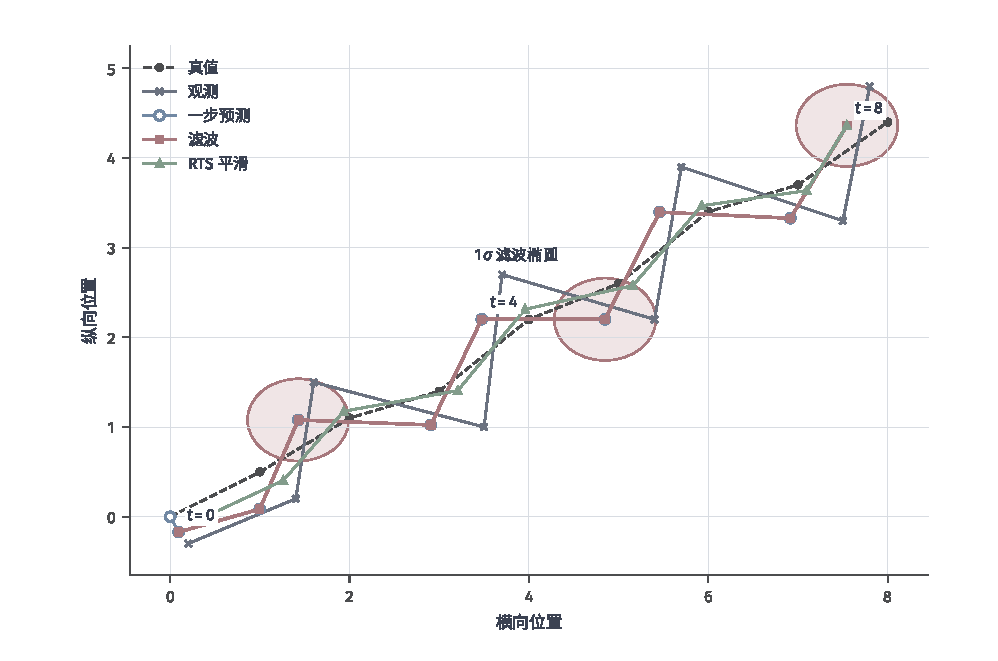
\includegraphics[width=159.059mm]{figures/06-probabilistic-graphical-models/04-models/matplotlib/pgm-dynamic-kalman-trajectory/figure.pdf}
  \caption{人工二维轨迹上的Kalman滤波与RTS平滑。黑色虚线为真值，灰叉为观测，蓝色空心点为观测前预测，红色方点为在线滤波均值，绿色三角为读取全部九次观测的平滑均值。红色半透明椭圆在$t=2,5,8$处显示滤波不确定性，其半轴为各坐标$1$倍标准差；末时刻两类均值重合。图源保存全部参数和坐标，结果对应这组固定的随机游走假设与观测。}
  \label{fig:pgm-dynamic-kalman-trajectory}
\end{figure*}

例~\ref{ex:pgm-dynamic-kalman}第二时刻的更新也可以直接看密度（图~\ref{fig:pgm-dynamic-gaussian}）。观测似然集中在$2$附近，预测密度集中在$0.5$附近，相乘并归一化后，后验均值位于$1.4$。测量与预测共同约束同一状态，使后验方差缩小。

\begin{figure}[htbp]
  \centering
  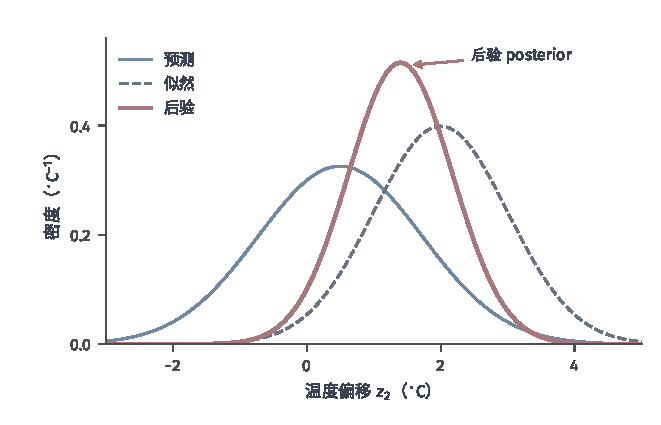
\includegraphics[width=105.412mm]{figures/06-probabilistic-graphical-models/04-models/matplotlib/pgm-dynamic-gaussian/figure.pdf}
  \caption{标量Kalman更新中的预测、似然与后验。蓝色实线表示预测$\mathcal{N}(0.5,1.5)$，灰色虚线表示对状态归一化的似然$\mathcal{N}(2,1)$，红色粗线表示后验$\mathcal{N}(1.4,0.6)$。图例区分三条曲线，红色引线标出后验。横轴为温度偏移，纵轴为密度。这里观测矩阵为$1$，观测似然对状态归一化后恰好形成图示高斯密度。}
  \label{fig:pgm-dynamic-gaussian}
\end{figure}

未知的线性映射和噪声协方差，可以用状态后验统计量来估计。线性高斯EM先计算完全数据对数似然需要的一阶、二阶矩，再拟合转移与观测分布。这与Baum--Welch按软计数学习的结构相同，区别在于连续状态用矩保存期望。当前参数下所需的统计量为
\begin{equation}
  \begin{aligned}
    \overline{\bm{z}}_t&=\bm{m}_{t\mid T},\\
    \bm{M}_t
      &:=\mathbb{E}[\bm{z}_t\bm{z}_t^\top\mid\bm{x}_{1:T}]
        =\bm{P}_{t\mid T}
          +\overline{\bm{z}}_t\overline{\bm{z}}_t^\top,\\
    \bm{M}_{t,t-1}
      &:=\mathbb{E}[\bm{z}_t\bm{z}_{t-1}^\top\mid\bm{x}_{1:T}]\\
      &=\bm{P}_{t,t-1\mid T}
          +\overline{\bm{z}}_t\overline{\bm{z}}_{t-1}^\top.
  \end{aligned}
  \label{eq:pgm-dynamic-em-moments}
\end{equation}
这些期望由同一组旧参数下的滤波和平滑结果给出，在整个M步中保持固定。Ghahramani和Hinton给出了线性系统EM的完全数据似然及相应充分统计量的推导\scite{pgm-dynamic-ghahramani1996}。

M步怎样使用这些矩，可以从残差展开看出。记转移残差$\bm r_t(\bm A)=\bm z_t-\bm A\bm z_{t-1}$，其期望外积为
\begin{equation}
  \begin{aligned}
    \bm{E}_t(\bm{A})
      &:=\mathbb{E}\bigl[
        \bm r_t(\bm A)\bm r_t(\bm A)^\top
        \mid\bm{x}_{1:T}\bigr]\\
      &=\bm{M}_t-\bm{A}\bm{M}_{t,t-1}^{\top}
        -\bm{M}_{t,t-1}\bm{A}^{\top}\\
      &\quad{}+\bm{A}\bm{M}_{t-1}\bm{A}^{\top}.
  \end{aligned}
  \label{eq:pgm-dynamic-transition-residual}
\end{equation}
观测残差的期望外积$\bm{D}_t(\bm{C})$同样展开为
\[
  \begin{aligned}
    \bm{D}_t(\bm{C})
      &=\bm{x}_t\bm{x}_t^\top
        -\bm{C}\overline{\bm{z}}_t\bm{x}_t^\top
        -\bm{x}_t\overline{\bm{z}}_t^\top\bm{C}^\top\\
      &\quad{}+\bm{C}\bm{M}_t\bm{C}^\top.
  \end{aligned}
\]
转移与观测的高斯对数密度包含协方差行列式和加权残差二次型。将二次型写成迹、再取后验期望，EM辅助目标为
\begin{equation}
  \begin{aligned}
    \mathcal Q
      &=-\frac{T-1}{2}\log|\bm Q|
        -\frac12\sum_{t=2}^{T}
          \operatorname{tr}\{\bm Q^{-1}\bm E_t(\bm A)\}\\
      &\quad{}-\frac{T}{2}\log|\bm R|
        -\frac12\sum_{t=1}^{T}
          \operatorname{tr}\{\bm R^{-1}\bm D_t(\bm C)\}\\
      &\quad{}+\text{初始项}+\text{常数}.
  \end{aligned}
  \label{eq:pgm-dynamic-lgssm-q}
\end{equation}
辅助目标把M步分成线性回归和协方差估计。回归使用完整后验二阶矩，因此平滑均值之外的状态不确定性也进入残差与参数更新。

当$T\geq2$、观测完整且相关二阶矩和可逆时，对$\bm A$求导得到回归的正规方程
\[
  \bm A^{(k+1)}\sum_{t=2}^{T}\bm M_{t-1}
    =\sum_{t=2}^{T}\bm M_{t,t-1}.
\]
观测映射满足相同形式的回归方程。先更新两个映射，再用新映射计算期望残差，得到
\begin{equation}
  \begin{aligned}
    \bm A^{(k+1)}
      &=\left(\sum_{t=2}^{T}\bm M_{t,t-1}\right)
        \left(\sum_{t=2}^{T}\bm M_{t-1}\right)^{-1},\\
    \bm C^{(k+1)}
      &=\left(\sum_{t=1}^{T}
        \bm x_t\overline{\bm z}_t^\top\right)
        \left(\sum_{t=1}^{T}\bm M_t\right)^{-1},\\
    \bm Q^{(k+1)}
      &=\frac{1}{T-1}\sum_{t=2}^{T}
        \bm E_t(\bm A^{(k+1)}),\\
    \bm R^{(k+1)}
      &=\frac{1}{T}\sum_{t=1}^{T}
        \bm D_t(\bm C^{(k+1)}).
  \end{aligned}
  \label{eq:pgm-dynamic-lgssm-m-step}
\end{equation}
对$\bm Q^{-1}$或$\bm R^{-1}$求导即可得到协方差更新，例如转移项满足$(T-1)\bm Q=\sum_t\bm E_t$。单条序列的初始参数更新为$\bm m_0^{(k+1)}=\overline{\bm z}_1$、$\bm P_0^{(k+1)}=\bm P_{1\mid T}$。对$n$条独立序列，$\bm m_0^{(k+1)}$取初始平滑均值的平均，$\bm P_0^{(k+1)}$取各初始平滑协方差与初始均值相对总体均值外积之和的平均。转移残差按$\sum_{\ell=1}^{n}(T_\ell-1)$归一化，观测残差按$\sum_{\ell=1}^{n}T_\ell$归一化。初始协方差这样同时保存序列内部的不确定性和各序列起点之间的差异。

将例~\ref{ex:pgm-dynamic-kalman}的平滑结果代入，得到$M_1=0.4+0.8^2=1.04$、$M_2=0.6+1.4^2=2.56$及$M_{2,1}=0.2+1.4\times0.8=1.32$。旧参数$A=C=Q=R=1$下算出的这组矩，给出一次无约束M步：
\[
  \begin{aligned}
    A^{(k+1)}&=1.32/1.04=33/26,\\
    C^{(k+1)}&=(1\times0.8+2\times1.4)/(1.04+2.56)=1,\\
    Q^{(k+1)}&=2.56-1.32^2/1.04=23/26,\\
    R^{(k+1)}&=(1^2+2^2-3.6)/2=0.7.
  \end{aligned}
\]
初始均值与方差分别变为$0.8$和$0.4$。更新得到$A^{(k+1)}>1$，说明无约束极大化可以选择增长的动力学；只有两个观测时，全部系统参数的识别还缺少数据支持。若目标要求稳定动力学，可在$\bm A$的谱半径上施加约束，并求解对应M步。

每轮EM完成滤波、平滑和矩的累计，固定维度时成本随总序列长度线性增长。可以结合似然增量与迭代上限停止，并比较多组初值的观测预测。二阶矩和奇异时，回归可能有多个解；协方差落到退化边界时，需要处理低维支撑。协方差下界、先验、已知噪声结构或固定参数可以约束这些问题，对应目标和更新也随之改变。

连续状态的坐标也有等价表示。对任意可逆矩阵$\bm H$，改用$\widetilde{\bm z}_t=\bm H\bm z_t$，并同时变换$\widetilde{\bm A}=\bm H\bm A\bm H^{-1}$、$\widetilde{\bm C}=\bm C\bm H^{-1}$、$\widetilde{\bm Q}=\bm H\bm Q\bm H^\top$和初始分布，观测分布保持不变。把某个坐标解释成温度或磨损程度，需要测量关系等额外约束。若一个非零方向始终不被$\bm C,\bm C\bm A,\ldots$观测到，数据对该方向的约束还可能不足。因此，后验计算、状态识别和长期误差控制分别依赖相应的模型条件。

单一线性机制适合的响应范围终究有限。下一小节仍保留连续状态，放开线性或高斯条件，考察后验积分怎样近似；由离散模式选择不同连续机制的另一种结构，则在第~\ref{sec:pgm-dynamic-mixed}节单独建立。

\subsection{非线性或非高斯的连续状态建模}
\label{sec:pgm-dynamic-nonlinear-model}

非线性动力学以及偏斜、离群点或离散跳变等噪声特征，可以用更一般的状态空间模型表示。具有加性噪声结构时，写为
\begin{equation}
  \bm z_t=f_t(\bm z_{t-1})+\bm\varepsilon_t,\qquad
  \bm x_t=h_t(\bm z_t)+\bm\eta_t.
  \label{eq:pgm-dynamic-nonlinear}
\end{equation}
直接指定转移和观测分布，还可以表示非加性、非高斯机制。Bayes递推式~\eqref{eq:pgm-dynamic-bayes-filter}依然适用，但单个高斯通常无法精确保存更新后的后验。下列方法分别在局部函数、积分矩或路径后验上近似，由此保留不同的信息。

转移函数、观测函数、噪声分布和初态仍共同构成模型；若它们依赖待估参数，就分别写为$f_{t,\bm\theta}$、$h_{t,\bm\theta}$及相应参数化密度。当前分支只讨论连续状态，离散模式与连续量的组合另见下一节。观测似然目标仍是
\begin{equation}
  \ell_{\mathrm{NL}}(\bm\theta)
    =\sum_n\log\int p_{\bm\theta}(\bm z_1)
      \prod_{t=2}^{T_n}p_{\bm\theta}(\bm z_t\mid\bm z_{t-1})
      \prod_{t=1}^{T_n}p_{\bm\theta}(\bm x_t^{(n)}\mid\bm z_t)
      \,\mathrm d\bm z_{1:T_n}.
  \label{eq:pgm-dynamic-nonlinear-objective}
\end{equation}
困难在于路径积分一般不再有高斯闭式。若采用近似EM，E步近似整段后验的初态、转移及观测统计，M步优化这些期望构成的辅助目标；一般非线性参数化要用数值优化，不能直接沿用线性回归更新。先明确以下工具各自返回什么状态分布，再决定它是否提供学习所需的整段统计。

一旦转移或观测函数非线性，高斯经过它一般不再是高斯，精确闭合被打破。最直接的补救是工程上常用的一阶近似：在当前均值处把非线性函数\emph{泰勒展开}到一阶、用其Jacobian当作线性化矩阵，于是这一步又能套用Kalman公式。它简单廉价，但只有在后验很集中、线性化误差可忽略时才准。在当前估计附近用一阶线性函数近似动力学和观测函数，就可以继续传播高斯均值与协方差。这形成\term{扩展Kalman滤波}（extended Kalman filter, EKF）。对加性高斯噪声，记$\bm F_t$为$f_t$在$\bm m_{t-1\mid t-1}$处的Jacobian，$\bm H_t$为$h_t$在预测均值处的Jacobian，预测计算为
\[
  \begin{aligned}
    \bm m_{t\mid t-1}&\approx f_t(\bm m_{t-1\mid t-1}),\\
    \bm P_{t\mid t-1}
      &\approx\bm F_t\bm P_{t-1\mid t-1}\bm F_t^\top+\bm Q_t,\\
    \bm S_t&\approx\bm H_t\bm P_{t\mid t-1}\bm H_t^\top+\bm R_t.
  \end{aligned}
\]
观测更新以$h_t(\bm m_{t\mid t-1})$为预测读数，以$\bm P_{t\mid t-1}\bm H_t^\top\bm S_t^{-1}$为增益。函数可微、后验集中在线性化有效区域时，局部函数及其矩的近似较为适用。初值偏离、强曲率或分离的后验峰会削弱这种局部表示。

EKF只在一个点上做线性化，强曲率时偏差很大，还要求算导数。无迹变换换一个思路：与其近似函数，不如挑少数几个精心选取的“代表点”（它们恰好匹配输入高斯的均值和协方差），让这些点\emph{原样}通过真正的非线性函数，再用变换后的点加权估计输出的均值和协方差，从而在不求导的情况下捕捉到一部分曲率。也可以让少量代表点直接经过非线性函数，用输出点估计变换后的矩。\term{无迹变换}（unscented transform, UT）选择确定性点来匹配输入均值与协方差，因而省去Jacobian计算。给定$q$维高斯近似$\mathcal N(\bm m,\bm P)$，取$\bm L\bm L^\top=\bm P$、$\kappa>0$，一种$2q+1$点规则为
\[
  \begin{aligned}
    \bm\chi_0&=\bm m,&w_0&=\frac{\kappa}{q+\kappa},\\
    \bm\chi_i&=\bm m+\sqrt{q+\kappa}\bm L_{:,i},
      &w_i&=\frac{1}{2(q+\kappa)},\\
    \bm\chi_{q+i}&=\bm m-\sqrt{q+\kappa}\bm L_{:,i},
      &w_{q+i}&=\frac{1}{2(q+\kappa)},
  \end{aligned}
\]
这里$i=1,\ldots,q$。对称点及其权重恰好恢复输入的$\bm m,\bm P$。经过$f$后，加权均值$\widehat{\bm\mu}=\sum_iw_i f(\bm\chi_i)$和协方差$\sum_iw_i(f(\bm\chi_i)-\widehat{\bm\mu})(f(\bm\chi_i)-\widehat{\bm\mu})^\top$近似输出矩。将这一规则用于预测状态、预测观测和两者的交叉协方差，再按高斯分布条件化，得到\term{无迹Kalman滤波}（unscented Kalman filter, UKF）。

例如$Z\sim\mathcal N(0,1)$经过$f(Z)=Z^2$。在$0$处，函数值和导数均为$0$，EKF给出的均值、方差都是$0$，精确结果则为$1$和$2$。取$q=1,\kappa=2$，代表点$0,\sqrt3,-\sqrt3$对应权重$2/3,1/6,1/6$，输出为$0,3,3$，加权后恰好恢复均值$1$、方差$2$。这个例子展示了代表点怎样捕捉均值附近的曲率。对其他函数，积分矩仍有近似误差；UKF还将条件后验压缩成一个高斯，分离的多个峰因此会丢失。Särkkä和Svensson讨论了EKF、UT及平滑扩展的条件与算法\scite{pgm-dynamic-sarkka2023}。

EKF、UKF都把后验强行压成一个高斯，遇到多峰（状态有几个互斥的可能解释）时会失效。另一类做法不去逐时刻递推某个特定形式，而是直接为\emph{整条状态路径}挑选一个计算得起的近似分布，用第7章的变分思想让它尽量贴近真实后验，从而能保留多峰或跨时刻相关等更丰富的结构。整段状态重建或参数学习还可以直接近似路径后验。\term{变分状态估计}（variational state estimation）选择可计算的路径分布$q_{\bm\phi}(\bm z_{1:T}\mid\bm x_{1:T})$，通过最大化证据下界拟合它（第~\ref{chap:pgm-variational}章）。在线性或局部二次近似下，结构化高斯族可保留相邻时刻的相关性；在下一节的切换系统中，这个思路还可扩展为离散模式链和连续状态链的联合近似。近似族确定了哪些依赖和后验形状能够保存。

对单条序列，其路径变分目标具体为
\begin{equation}
  \begin{aligned}
  \mathcal L(\bm\theta,\bm\phi;\bm x)
    &=\mathbb E_{q_{\bm\phi}(\bm z\mid\bm x)}
        \biggl[\log p_{\bm\theta}(\bm z_1)
        +\sum_{t=2}^{T}\log p_{\bm\theta}(\bm z_t\mid\bm z_{t-1})\\
    &\qquad{}+\sum_{t=1}^{T}\log p_{\bm\theta}(\bm x_t\mid\bm z_t)
        -\log q_{\bm\phi}(\bm z\mid\bm x)\biggr].
  \end{aligned}
  \label{eq:pgm-dynamic-path-elbo}
\end{equation}
共享编码器可以由读数给出近似分布参数，也可以为每条序列直接设置局部变分参数；$\bm\phi$表示相应的待优化量。固定$\bm\theta$、只更新$\bm\phi$是近似状态推断；联合训练则最大化各记录下界之和，交替或联合更新两组参数。梯度中的期望需按近似族解析计算、重参数化或采样估计，并满足相应的可微与可积条件。联合学习时，下界由观测对数似然和近似后验误差共同决定，优化过程中两者都可能变化；模型的预测表现仍需单独评价。

当后验多峰、偏斜、甚至任意形状时，用一个高斯或几个参数都难以刻画，最普适的办法是退回到第8章的蒙特卡洛思想：用一大把带权重的状态\emph{样本（粒子）}来非参数地表示整个后验分布，多个峰可以同时被不同粒子占据，权重则按观测不断更新。分离的后验峰对应不同状态解释，可以用一组样本同时保留。\term{粒子滤波}（particle filtering）以带权状态样本近似滤波分布。设粒子数$n$，第$i$个粒子为$\bm z_{t,i}$，按$q_t(\bm z_t\mid\bm z_{t-1,i},\bm x_t)$提议。在尚未重采样的一步，权重更新为
\[
  w_{t,i}\propto w_{t-1,i}
    \frac{p(\bm x_t\mid\bm z_{t,i})
      p(\bm z_{t,i}\mid\bm z_{t-1,i})}
      {q_t(\bm z_{t,i}\mid\bm z_{t-1,i},\bm x_t)}.
\]
若先按旧权重重采样祖先，祖先选择已计入旧权重，新权重只需当前的重要性比率。序贯重要性更新及带重采样的自举滤波见式~\eqref{eq:pgm-sampling-sis-weight}与算法~\ref{alg:pgm-sampling-bootstrap}。它们用样本和加权和代替难以解析的积分。转移先验提议可约去权重中的转移项；观测集中时，却可能让大量粒子落在低似然区域。每步需要约$n$次转移、似然求值以及重采样，维度与时间跨度影响所需粒子数。固定$n$时，应检查权重集中和样本覆盖。

长期重采样可能使许多粒子共享早期祖先，降低过去路径的多样性。因此，离线平滑和EM还需粒子平滑或其他路径后验方法，计算选择取决于任务需要保留的状态或路径不确定性。



\section{离散模式与连续状态的联合建模}
\label{sec:pgm-dynamic-mixed}

前面要么用离散链（HMM，状态是模式但无法刻画模式内细腻的连续变化），要么用连续状态空间（LGSSM，全程服从同一套线性动态，无法表达“系统在几套截然不同的运行机制之间切换”）。但很多真实过程两者兼有：设备在升温、恒温、冷却等\emph{离散模式}间切换，而在每个模式内部温度又近似服从各自的\emph{线性高斯}动态。把两层结合起来，让离散模式去选择当前用哪一套连续动态方程，就得到切换线性动态系统。有些设备既有升温、恒温等离散运行模式，又有各模式内连续变化的温度。只选择离散或连续一种状态，会把两种不同的信息挤在同一表示里。我们可以让离散模式选择局部连续机制，保留两层不确定性，并组合前面两类模型的计算。

升温、恒温和冷却可能各自近似线性，却使用不同的转移参数。\term{切换线性动态系统}（switching linear dynamical system, SLDS）引入离散模式$S_t\in\{1,\ldots,L\}$，按模式选择连续转移与观测机制。这里$S_t$表示运行模式，与四节点例中传感器失灵变量$S$分别定义。一个常见形式为
\begin{equation}
  \begin{aligned}
    p(s_t\mid s_{t-1})&=\omega_{s_{t-1},s_t},\\
    \bm z_t\mid\bm z_{t-1},s_t
      &\sim\mathcal N(\bm A_{s_t}\bm z_{t-1},\bm Q_{s_t}),\\
    \bm x_t\mid\bm z_t,s_t
      &\sim\mathcal N(\bm C_{s_t}\bm z_t,\bm R_{s_t}),
  \end{aligned}
  \label{eq:pgm-dynamic-switching}
\end{equation}
指定$p(s_1)$与条件高斯初始分布$p(\bm z_1\mid s_1)=\mathcal N(\bm z_1;\bm m_{0,s_1},\bm P_{0,s_1})$后，就能按这些局部机制生成完整序列。图~\ref{fig:pgm-dynamic-switching}显示模式对连续状态与观测的影响。推断时模式也未知，需同时保留可能模式与各模式下的状态不确定性。

\begin{figure}[htbp]
  \centering
  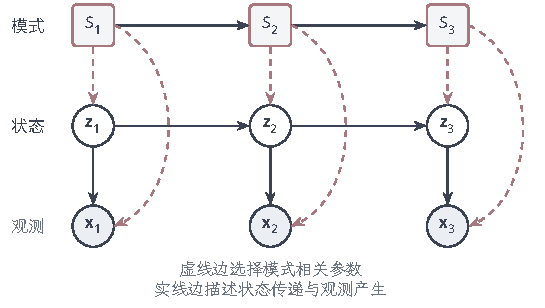
\includegraphics[width=92.276mm]{figures/06-probabilistic-graphical-models/04-models/tikz/pgm-dynamic-switching/figure.pdf}
  \caption{切换系统的三层依赖。方形节点表示离散模式，空心圆表示连续状态，填色圆表示观测。每条完整模式路径对应一组线性高斯递推；到达相同当前模式的不同历史仍可产生不同高斯后验。}
  \label{fig:pgm-dynamic-switching}
\end{figure}

这些局部分布需要组合成同一个联合模型，才能确定哪些模式路径进入训练。完整结构与目标为
\begin{equation}
  \begin{aligned}
    p_{\bm\theta}(s,z,x)
      &=p_{\bm\theta}(s_1)p_{\bm\theta}(\bm z_1\mid s_1)
        \prod_{t=2}^{T}p_{\bm\theta}(s_t\mid s_{t-1})
                           p_{\bm\theta}(\bm z_t\mid\bm z_{t-1},s_t)\\
      &\qquad{}\times\prod_{t=1}^{T}
                           p_{\bm\theta}(\bm x_t\mid\bm z_t,s_t),\\
    \ell_{\mathrm{SLDS}}(\bm\theta)
      &=\sum_n\log\sum_{s_{1:T_n}}\int
                   p_{\bm\theta}(s,z,x^{(n)})\,\mathrm d\bm z_{1:T_n}.
  \end{aligned}
  \label{eq:pgm-dynamic-switching-objective}
\end{equation}
模式概率以及每种模式的映射、噪声与初态都是待估参数。式中的求和保留运行模式的不确定性，积分保留同一模式路径内的连续不确定性。只保留最可能模式再拟合连续量，会改变此处的似然目标。

固定模式历史$s_{1:t}$时，连续状态后验为高斯；换一条历史，均值和协方差一般随之改变。精确滤波把这些历史加在一起，最多形成$L^t$个高斯分量。合并、剪枝或限制每种当前模式的分量数，以近似换取可控成本。EM同时需要模式转移期望计数与各模式的连续二阶矩，E步的混合推断质量因而直接影响学习。

更新所需统计量可以从完全数据分解直接读出。以下期望均在旧参数的整段联合平滑后验下计算，$\sum_{n,t\geq2}$表示汇总每条序列内部的转移。模式转移的更新为
\[
  \omega_{i,j}^{\mathrm{new}}
    =\frac{\sum_{n,t\geq2}p(S_{t-1}=i,S_t=j\mid x^{(n)})}
           {\sum_{n,t\geq2}p(S_{t-1}=i\mid x^{(n)})}.
\]
对当前模式$j$，先累计由$\mathbf1\{S_t=j\}$加权的连续矩和模式占用量：
\[
  \begin{aligned}
    \bm U_j&=\sum_{n,t\geq2}\mathbb E[
       \mathbf1\{S_t=j\}\bm z_{t-1}\bm z_{t-1}^{\top}\mid x^{(n)}],\\
    \bm V_j&=\sum_{n,t\geq2}\mathbb E[
       \mathbf1\{S_t=j\}\bm z_t\bm z_{t-1}^{\top}\mid x^{(n)}],\\
    w_j&=\sum_{n,t\geq2}p(S_t=j\mid x^{(n)}).
  \end{aligned}
\]
于是局部回归与噪声更新为
\begin{equation}
  \begin{aligned}
    \bm A_j^{\mathrm{new}}&=\bm V_j\bm U_j^{-1},\\
    \bm r_{t,j}&=\bm z_t-\bm A_j^{\mathrm{new}}\bm z_{t-1},\\
    \bm Q_j^{\mathrm{new}}
      &=\frac{1}{w_j}\sum_{n,t\geq2}\mathbb E[
       \mathbf1\{S_t=j\}\bm r_{t,j}\bm r_{t,j}^{\top}\mid x^{(n)}].
  \end{aligned}
  \label{eq:pgm-dynamic-switching-update}
\end{equation}
这与线性高斯EM使用相同的回归与残差原理，但每项由当前模式的后验概率加权。观测映射$\bm C_j$的回归分别需要观测与状态的后验交叉矩，以及状态的后验二阶矩：
\[
 \begin{aligned}
  &\sum_{n,t}\bm x_t^{(n)}\mathbb E[
          \mathbf1\{S_t=j\}\bm z_t^{\top}\mid x^{(n)}],\\
  &\sum_{n,t}\mathbb E[
          \mathbf1\{S_t=j\}\bm z_t\bm z_t^{\top}\mid x^{(n)}].
 \end{aligned}
\]
第一项乘第二项的逆矩阵给出$\bm C_j$的更新。$\bm R_j$则对观测残差外积按模式占用量归一化。初态概率由各起点的模式边缘平均；每种模式的初始均值与协方差由起点的加权一二阶矩更新。

这些更新要求相应加权矩可逆、模式占用量非零，且没有改变自由协方差设定的额外约束。训练依次执行混合平滑、累计统计、更新模式概率和连续参数，再检查观测目标或相应近似目标；近似E步不能直接继承精确EM的似然单调保证。只有一个模式时，求和消失并退回LGSSM；一般SLDS的连续状态不能精确压成有限个离散类别，因此通常不能化为有限状态HMM。

在式~\eqref{eq:pgm-dynamic-switching}中，可以只抽样离散模式路径，每个粒子内部按给定模式历史运行精确Kalman递推。这种Rao--Blackwell化利用条件线性高斯结构来减少采样对象（第~\ref{chap:pgm-sampling}章）。

每个粒子还必须携带自己的模式历史条件下的高斯参数；只知道当前模式并不足以选定唯一高斯后验。粒子滤波返回当前状态近似，离线EM还需要整段平滑下的模式计数与相邻连续矩，不能用各时刻滤波均值替代。

\section{状态表示、查询与模型选择}
\label{sec:pgm-dynamic-comparison}

本章模型沿状态可见与否、离散或连续、记忆长度、单链或多链、线性或非线性、是否含离散模式切换等维度变化。下面把它们放回同一套状态空间框架，按要描述的状态、要回答的查询以及对应的推断与学习代价横向比较，作为具体任务选型的依据。对同一条报警序列，模型选择需要同时回答状态表达什么、读取哪些证据以及如何学习机制。先综合各模型之间的结构关系，再讨论这些选择对查询和评价的影响。

\subsection{同一骨架上的模型特例与组合}
\label{sec:pgm-dynamic-model-relations}

比较动态有向模型时，先固定要描述的状态与要回答的查询：状态是否可见、取离散值还是连续值，转移保留多长历史，推断可读取哪些时刻的证据。表~\ref{tab:pgm-dynamic-models}据此并列各类模型的条件和计算。DBN作为共同表示框架适用于各行，具体差别来自状态空间、局部分布和依赖假设。

\begin{table*}[htbp]
  \centering
  \small
  \begin{tabularx}{\linewidth}{@{}p{25mm}p{23mm}p{29mm}p{27mm}X@{}}
    \toprule
    模型 & 状态可见性与空间 & 转移假设 & 常见查询 & 推断与学习 \\
    \midrule
    有限Markov链 & 可见、离散 & 按当前状态给出下一状态分布 & 多步预测、长期分布 & 矩阵递推；可见转移计数 \\
    HMM & 隐藏、离散 & 一阶链，几何停留时间 & 滤波、平滑、整条路径 & 前向--后向、Viterbi；Baum--Welch \\
    高阶HMM与HSMM & 隐藏、离散或分段状态 & 更长历史或显式持续时间 & 路径与片段边界 & 扩充状态或片段动态规划；期望计数 \\
    因子HMM & 多条隐藏离散链 & 先验转移分开，观测耦合 & 联合滤波与平滑 & 联合表可精确但指数增长；变分或采样 \\
    线性高斯模型 & 隐藏、连续 & 线性转移与独立高斯噪声 & 状态分布、预测密度 & Kalman滤波、RTS平滑；二阶矩EM \\
    切换线性系统 & 隐藏、离散与连续混合 & 模式选择线性动态 & 模式与连续状态联合查询 & 高斯混合枚举一般指数增长；混合约简或条件粒子方法 \\
    一般状态空间模型 & 隐藏、连续或混合 & 非线性、非高斯等 & 滤波、平滑及预测风险 & 局部线性化、矩近似、变分或粒子方法 \\
    \bottomrule
  \end{tabularx}
  \caption{动态有向模型的状态、转移与计算。各类模型均需指定初始分布，线性高斯精确递推还需高斯初态。近似方法可按后验形状和查询要求组合选择。}
  \label{tab:pgm-dynamic-models}
\end{table*}

从共同框架看，DBN允许一般切片内与跨片依赖，状态空间分解进一步把历史影响集中到一个状态并令当前观测由它产生。HMM与LGSSM随后分别限制状态空间和局部分布，而高阶、显式时长及因子结构改变状态记忆、片段或组成。SLDS把离散选择与连续机制放在同一联合分布中。这些是结构、特例或组合关系；Kalman、Viterbi和粒子算法则是固定模型后回答不同查询的计算方法。

学习目标也要和结构一起比较。可见链最大化完整状态似然，隐藏状态模型最大化观测边缘似然；计算这类目标时，离散模型需要路径期望计数，线性高斯模型需要后验一二阶及相邻矩，混合模型同时需要两者。路径变分法改为优化显式下界。即使两种模型都调用EM或前向消息，这也不保证它们的观测变量、目标和学习统计相同。

有限状态动态规划和Kalman递推每次都将过去压缩成固定大小的精确消息。前者保存$K$个状态概率，后者保存均值向量和协方差矩阵，因而维度固定时，总成本随时间长度线性增长。接口固定仍可能带来昂贵消息：因子HMM需记录$K^M$种联合配置，切换系统的高斯分量又随模式历史增多。评价成本时，应同时给出序列长度、接口维度和消息表示。

\subsection{推断、学习与评价对应不同问题}
\label{sec:pgm-dynamic-evaluation}

证据可用的时刻决定查询算法。在线控制按当前和过去读数滤波，事后检修则可借助未来证据平滑，两者应分别评价。若损失按逐时刻误判数累计，平滑边缘给出相应最优决策；要求完整路径满足转移限制时，则优化联合解释。连续联合高斯后验的均值也是联合密度众数，混合后验中这两个对象却可能分离，平均值甚至位于分量之间的低密度区域。

误差诊断需要同时检查模型和计算。HMM即使精确推断，也可能因状态过少或持续时间假设偏差而预测失配；EKF还增加了局部线性化误差。比较方法时，固定训练与测试的时间边界，以及一步或多步预测目标，再报告预测对数密度与计算成本；有状态参考值时，可同时评价状态误差和后验不确定性覆盖。按时间保持数据边界，才能评价面向未来的预测；打乱时间点或提前读取未来观测会改变这个任务。

共享参数把多个时刻的数据用于估计同一局部机制，在共享假设适用时减少了待估自由度。运行环境变化后，旧的齐次机制可能失配；已知输入、时变参数或模式切换可表示这种变化，新增机制也需要相应数据来识别。选择模型时，先确定任务所需依赖，再检查状态后验的表示与计算成本，使表达范围、可估计性和推断方法相互匹配。

\section{本章小结}
\label{sec:pgm-dynamic-summary}

动态有向分解把过去对未来的影响集中到时间接口上，使新观测能够逐步并入当前判断。DBN规定依赖模板，Markov性规定给定状态后哪些历史可被压缩，时间齐次与参数共享规定机制的复用方式，平稳性规定过程分布在时间平移下的变化。明确各项条件，才能知道递推中保存的消息代表什么。

有限隐藏状态用前向--后向消息累加路径概率，用Viterbi前驱表恢复最优路径，再由Baum--Welch按后验期望计数学习。线性高斯系统用均值和协方差精确保存状态分布，经Kalman滤波与RTS平滑取得一阶、二阶矩，再拟合局部映射与噪声。这两条路线都先以局部消息完成全局推断，再把后验统计量交给参数学习。

设备的当前报警判断、故障追溯和整段工况解释分别对应滤波、平滑和路径查询。状态增多、持续时间复杂或模式与连续动态混合时，精确消息成本上升，局部高斯、变分和粒子方法在不同位置近似。模型的表达假设决定可描述的演化规律，推断与学习决定怎样从观测取得判断，时间隔离的预测评价则检验它在新数据上的适用性。

\Needspace{8\baselineskip}
\paragraph{扩展阅读}
Bishop的PRML第13章从顺序数据展开HMM与线性动态系统，Murphy的教材进一步讨论滤波、平滑和状态估计。阅读时可沿同一观测序列比较各查询的证据范围，并追踪后验消息怎样变成参数学习所需的统计量\scite{bishop2006,pgm-murphy2012}。

\chapter{动态无向模型}
\label{chap:pgm-dynamic-undirected}

设备先后出现两次高温报警，我们希望判断它们是否属于同一段持续故障。若几个相邻设备也同时报警，还需要考虑空间上的共同变化。上一章用状态转移和观测生成机制描述这些关系；也可以直接为“相邻时刻状态相容”“同一时刻设备状态相容”规定权重，再比较整段状态的所有候选配置。后一种做法得到沿序列展开的无向模型。

无向边不否认时间的先后，只是不把局部相容权重解释为从前一状态生成后一状态的条件概率。已知整段读数、只预测故障标签时，还可以把读数固定在势函数中，对标签序列单独归一化。下面先建立这两种归一化的共同形式，再分别讨论联合状态建模和条件序列预测，说明状态、片段与多状态耦合怎样改变推断和学习。

\section{动态无向模型的共同形式}
\label{sec:pgm-dynamic-undirected-common}

把第$t$个位置的一组状态记为$\bm V_t$，序列长度为$T$；输入读数另记为$\bm x_{1:T}$。一个时间切片可以只有一个状态，也可以包含多个设备或多个标签。局部因子既可连接同一片内的变量，也可跨相邻片；重复同一种连接及参数，就形成时间模板。它描述随机变量沿序列的组织，不要求图结构随时间改变。

先考虑相邻切片的作用。令$a_{\bm\theta,t}(\bm v_t)$为片内得分，$b_{\bm\theta,t}(\bm v_{t-1},\bm v_t)$为跨片得分；首尾边界偏好计入相应$a$。整段联合分布为
\begin{equation}
  \begin{aligned}
    F_{\bm\theta}(\bm v_{1:T})
      &=\sum_{t=1}^T a_{\bm\theta,t}(\bm v_t)
          +\sum_{t=2}^T b_{\bm\theta,t}
                         (\bm v_{t-1},\bm v_t),\\
    p_{\bm\theta}(\bm v_{1:T})
      &=\frac{\exp F_{\bm\theta}(\bm v_{1:T})}
                    {Z_{\bm\theta,T}}.
  \end{aligned}
  \label{eq:pgm-dynamic-undirected-joint}
\end{equation}
记$\mathcal V_t$为第$t$片状态空间，$\mu_t$为相应的计数测度或连续状态的Lebesgue测度，令$\mu=\bigotimes_{t=1}^T\mu_t$，则
\[
  Z_{\bm\theta,T}=\int_{\prod_t\mathcal V_t}
     \exp F_{\bm\theta}(\bm v_{1:T})\,\mu(\mathrm d\bm v_{1:T}).
\]
它对全部建模状态求和或积分。得分是负能量，各个指数得分是局部势，无须分别归一化；其概率语义承接第~\ref{chap:pgm-energy-models}章。有限离散空间及有限得分保证配分函数正且有限；连续状态则需要尾部可积，后面的高斯模型用正定二次能量满足这一条件。

如果读数已知、未知量是标签$\bm Y_{1:T}$，局部得分可以依赖输入，归一化只覆盖标签：
\begin{equation}
  p_{\bm\theta}(\bm y_{1:T}\mid\bm x_{1:T})
    =\frac{\exp F_{\bm\theta}(\bm y_{1:T};\bm x_{1:T})}
                  {Z_{\bm\theta,T}(\bm x_{1:T})}.
  \label{eq:pgm-dynamic-undirected-conditional}
\end{equation}
这里$Z_{\bm\theta,T}(\bm x_{1:T})$对标签的乘积状态空间求和或积分，输入固定为查询条件。输入特征可以使用已取得的过去、当前及未来读数；这不等于模型给输入规定了生成分布。若任务只能在线使用过去读数，就必须据此限制可用特征与查询信息，不能把整段输入下的预测当作在线预测。

在切片之间切开图，所有跨界因子共同涉及的未知变量构成时间接口。求和消息保留接口配置的权重，最大化消息保留最优配置；单标签链的接口只是一个标签，多设备耦合或高阶历史则可能需要多个变量。决定计算规模的是接口状态数及其可利用的因子分解，而不只是序列长度。连续模型若具有高斯闭合性，接口消息可以由均值、精度等有限参数表示。

本章先为每个有限$T$定义分布。即使每一段都复用相同局部势，截去末端后的边缘也未必等于另行归一化的短链：对末状态求和会留下一个依赖前端状态的边界权重。若要建立一致的无限随机过程，还须检查不同长度的边缘相容性。参数共享也只表示局部函数使用相同参数，不自动保证平稳性。

\section{联合动态无向模型}
\label{sec:pgm-dynamic-undirected-joint-models}

联合模型评价整段状态的概率。给定部分时刻的状态后，可以补全其余位置；需要生成序列时，还要从该联合分布采样。下面先让时间接口只含一个离散状态或一个连续向量，再增加同一时刻的空间相互作用。

\subsection{离散链式模型}
\label{sec:pgm-dynamic-undirected-discrete-chain}

\paragraph{模型结构}
持续故障的相邻状态通常比频繁跳变的状态更相容。令$S_t\in\{1,\ldots,K\}$，用正势$\phi_t(k)$评价单点状态，用$\psi_t(j,k)$评价相邻状态组合，联合权重为
\begin{equation}
  w(s_{1:T})=\phi_1(s_1)
             \prod_{t=2}^T\psi_t(s_{t-1},s_t)\phi_t(s_t),
  \qquad p(s_{1:T})=\frac{w(s_{1:T})}{\sum_{u_{1:T}}w(u_{1:T})}.
  \label{eq:pgm-dynamic-undirected-chain-weight}
\end{equation}
二值状态$S_t\in\{-1,+1\}$可取得分$\sum_t h_tS_t+\sum_{t\ge2}J_tS_{t-1}S_t$，得到Ising链。$J_t>0$提高同号配置的相对权重，$h_t$则指定单点偏好。Potts链将同号奖励改为$J_t\mathbf1\{S_{t-1}=S_t\}$，支持多类别状态。链式分解限制为局部相邻作用，不能表达任意长程约束；但局部耦合已经可以产生远处变量的边缘相关。

一个三位置教学例子取$\phi_t=1$、同号边势为$3$、异号为$1$。两条边都同号的两种配置各有权重$9$，只有一条边同号的四种配置各为$3$，两条边都异号的两种配置各为$1$，总权重是$32$。每个位置的正类边缘仍为$1/2$，相邻同号的概率却为$3/4$。把三个位置各自拟合成概率$1/2$的独立状态，会遗漏这项持续性。

\paragraph{推断}
前向消息汇总以某个状态结束的前缀，后向消息汇总该状态之后的后缀。令$\alpha_1(k)=\phi_1(k)$、$\beta_T(k)=1$，递推为
\begin{equation}
  \begin{aligned}
    \alpha_t(k)&=\phi_t(k)\sum_j\alpha_{t-1}(j)\psi_t(j,k),\\
    \beta_{t-1}(j)&=\sum_k\psi_t(j,k)\phi_t(k)\beta_t(k),\\
    Z&=\sum_k\alpha_T(k),\qquad
    p(S_t=k)=\alpha_t(k)\beta_t(k)/Z.
  \end{aligned}
  \label{eq:pgm-dynamic-undirected-chain-messages}
\end{equation}
固定某个已观测状态时，将其余状态的单点势置零，再执行同样递推，所得归一化分布就是状态补全的条件分布。最大积和回溯则求整段最可能状态，不能替代边缘概率。一般稠密边势下，前向、后向或最优序列解码均需$O(TK^2)$时间。

有限正链也能改写为有向Markov链，但转移需要吸收后缀权重：
\begin{equation}
  p(S_t=k\mid S_{t-1}=j)
     =\frac{\psi_t(j,k)\phi_t(k)\beta_t(k)}{\beta_{t-1}(j)},
     \quad t\ge2.
  \label{eq:pgm-dynamic-undirected-chain-transition}
\end{equation}
在给定前一状态后，前缀与后缀被该状态分隔，上式由条件概率的比值直接得到，分母正好是分子的状态和。初始分布为$\phi_1(k)\beta_1(k)/Z$。因此无向链与有向链可以表示相同有限序列分布；直接把$\psi_t$逐行归一化，通常却会丢掉状态偏好和后缀影响。即使势共享参数，转换后的转移也可能随距末端的位置变化。

\paragraph{参数学习}
设完整训练序列的得分为$F_{\bm\theta}=\bm\theta^\top\bm G$，$\bm G$汇总所有位置的单点与相邻状态特征。单条记录的对数似然梯度是
\[
  \bm G(s_{1:T})-\mathbb E_{p_{\bm\theta}}\bm G(S_{1:T}).
\]
第一项来自观测状态，第二项由消息给出的单点及相邻状态边缘计算。重复参数接收全部位置的统计和；统计和里的各项依赖，并不是独立训练样本。若某些状态未观测，第一项还须改为给定已知状态后的特征期望。近似该后验与近似模型期望是两项不同误差，通用学习推导见第~\ref{chap:pgm-parameter-learning}章。

\subsection{高斯链式模型}
\label{sec:pgm-dynamic-undirected-gaussian-chain}

\paragraph{模型结构}
温度或位移是连续量，状态还可能同时含多个坐标。对相邻差异及状态偏好使用二次评分，可以保留链结构并得到可解析的连续分布。令每片$\bm V_t\in\mathbb R^d$，把$\bm v_{1:T}$堆叠为$Td$维向量$\bm v$，取
\begin{equation}
  E(\bm v)=\tfrac12\bm v^\top\bm K\bm v-\bm h^\top\bm v,
  \quad \bm K=\bm K^\top\succ0,
  \qquad
  p(\bm v)=\mathcal N(\bm K^{-1}\bm h,\bm K^{-1}).
  \label{eq:pgm-dynamic-undirected-gaussian}
\end{equation}
$\bm h$是$Td$维线性得分参数，正定精度$\bm K$保证能量可积。只允许同片和相邻片关系时，$\bm K$是块三对角矩阵；非相邻块为零，表示给定其余状态后的条件独立。此类模型只表达单峰高斯序列分布，不能靠增加链长度产生非高斯多峰状态。

例如标量能量$E=\tfrac12av_1^2+\tfrac12q\sum_{t=2}^T(v_t-v_{t-1})^2$，$a,q>0$，先约束初始状态，再约束相邻差异。若去掉初始项，所有状态一起平移不改变能量，常数方向不受约束，不能在$\mathbb R^T$上归一化。这个例子说明平滑偏好本身并不足以定义合法联合分布。

线性高斯状态空间模型也可写成这种能量。初始高斯项与各转移高斯项的负对数相加，便得到块三对角精度；将观测层一并建立后，固定读数会再加入测量二次项。反过来，正定高斯链可以通过条件分布形成有向表示。两种表示可能对应同一有限序列分布，状态转移和空间条件关系强调的建模对象却不同（参见第~\ref{chap:pgm-dynamic}章）。

\paragraph{推断}
联合均值满足$\bm K\bm m=\bm h$。记对角块为$\bm D_t$，下邻块为$\bm B_t=\bm K_{t,t-1}$，线性项分块为$\bm h_t$。从前向后消元，定义$\bm S_1=\bm D_1$、$\bm r_1=\bm h_1$，并递推
\begin{equation}
  \begin{aligned}
    \bm S_t&=\bm D_t-\bm B_t\bm S_{t-1}^{-1}\bm B_t^\top,\\
    \bm r_t&=\bm h_t-\bm B_t\bm S_{t-1}^{-1}\bm r_{t-1}.
  \end{aligned}
  \label{eq:pgm-dynamic-undirected-gaussian-elimination}
\end{equation}
$\bm S_t$是消去前面状态后留给当前片的精度，$\bm r_t$是相应线性项；正定性保证各Schur补仍正定。逆矩阵记号表示解线性方程的作用，实际可用Cholesky分解完成，不必显式求逆。末端先求$\bm m_T=\bm S_T^{-1}\bm r_T$，再反向代入
\[
  \bm m_t=\bm S_t^{-1}
       (\bm r_t-\bm B_{t+1}^\top\bm m_{t+1}).
\]
给定右端状态后，左端条件均值是这个仿射形式；对右端后验求期望，便得到整个链的均值。

若部分坐标$\bm v_O$已知，把其余坐标记为$\bm V_U$，条件精度仍为$\bm K_{UU}$，线性项变为$\bm h_U-\bm K_{UO}\bm v_O$。这由将已知值代入二次能量、收集未知坐标的项得到；对剩余链执行消元，就能计算状态补全的均值与协方差。

学习和不确定性评价还需要协方差。记$\bm C_t=\operatorname{Cov}(\bm V_t)$，由条件高斯的全协方差公式可得
\begin{equation}
  \begin{aligned}
    \bm C_T&=\bm S_T^{-1},\\
    \bm C_t&=\bm S_t^{-1}
       +\bm S_t^{-1}\bm B_{t+1}^\top\bm C_{t+1}
                          \bm B_{t+1}\bm S_t^{-1},\\
    \operatorname{Cov}(\bm V_t,\bm V_{t+1})
      &=-\bm S_t^{-1}\bm B_{t+1}^\top\bm C_{t+1}.
  \end{aligned}
  \label{eq:pgm-dynamic-undirected-gaussian-moments}
\end{equation}
单片和相邻片的矩已足以计算链式二次特征。一般稠密$d\times d$块下，这些递推需$O(Td^3)$时间和$O(Td^2)$存储；若要求全部非相邻协方差，输出本身可占$O(T^2d^2)$空间。把局部矩查询与显式生成完整协方差混为一谈，会夸大前者的成本\scite{pgm-undirected-rue2005}。

\paragraph{参数学习}
完整记录给出$\bm V_t$及$\bm V_t\bm V_s^\top$的样本统计量；块三对角结构只需要$s=t$或$s=t+1$的二阶项。拟合自然参数$\bm K,\bm h$时，似然梯度比较观测统计与上述递推计算的模型统计，同时保持$\bm K\succ0$和指定稀疏模式。若按状态空间的转移矩阵、噪声协方差参数化，则沿用对应模型的学习约束；不同参数化的优化性质不能混用。

状态部分缺失时，用给定已知状态后的均值与协方差形成期望统计量，再执行学习更新。潜在坐标及共享参数还可能不可唯一解释，有限样本也可能不足以得到非退化协方差估计；正则化和可识别条件需要随拟合目标说明。高斯闭合性解决的是概率与矩计算，不自动保证任意参数学习问题都唯一可解。

\subsection{时空相互作用模型}
\label{sec:pgm-dynamic-undirected-spatiotemporal}

\paragraph{模型结构}
多个设备沿时间变化时，仅为每个设备建立独立链，会漏掉邻近设备同时过热的关系。令每片有$m$个状态$V_{t,i}$，固定空间邻接集合为$\mathcal E_s$。把空间关系和同一设备的时间持续性都加入得分：
\begin{equation}
  \begin{aligned}
    F(\bm v)= {}&\sum_{t,i}a_{t,i}(v_{t,i})
       +\sum_t\sum_{(i,j)\in\mathcal E_s}
                      c_{t,ij}(v_{t,i},v_{t,j})\\
       &+\sum_{t=2}^T\sum_i b_{t,i}(v_{t-1,i},v_{t,i}).
  \end{aligned}
  \label{eq:pgm-dynamic-undirected-spatiotemporal}
\end{equation}
整段联合分布仍按$e^F$归一化。空间势说明同一片内哪些状态相互作用，时间势说明哪些状态跨片相连；它们不要求输入测量存在有向生成关系。离散状态可以使用Ising、Potts或一般状态表，连续状态若使用可积二次能量，则得到稀疏时空高斯随机场。

\paragraph{推断}
把一片的全部状态合并，可以形式上得到一条向量状态链，却不能因此忽略接口规模。每设备有$K$个状态时，一片已有$K^m$种配置，朴素稠密片间递推需$O(TK^{2m})$时间。利用原空间图及跨片因子进一步分解，可能降低实际计算；精确消元的主要限制是诱导宽度。若宽度过大，可按第~\ref{chap:pgm-variational}、\ref{chap:pgm-sampling}章近似所需边缘或期望，并检查实际查询的误差。

高斯时空图即使成环，也可以利用正定精度的稀疏线性代数计算均值。消元时出现的填充决定分解成本，不能仅由原图边数推出线性复杂度。离散图上的环与高斯图上的环，因势函数的代数闭合性不同，带来的是不同计算问题。

\paragraph{参数学习}
空间共享参数汇总各位置的空间特征，时间共享参数汇总各设备的跨片特征，再与模型期望比较。完整设备阵列的一段轨迹构成一条训练记录；同段里的节点和时间片有依赖，样本单位仍应按数据收集机制确定。若依赖近似边缘计算梯度，优化停止还需结合推断误差检查，训练目标的小幅变化本身不足以确认模型期望已算准。

\section{条件动态无向模型}
\label{sec:pgm-dynamic-undirected-conditional-models}

只需根据读数判断故障标签时，可以直接建立标签的条件分布。线性链先表达逐点标签的相邻关系；半Markov模型把输出改为片段；多状态链保留多个标签之间的耦合；潜状态模型则在已标注的任务输出之外增加内部解释。这些选择可以组合，下面按各自补充的职责展开。
\subsection{线性链条件随机场}
\label{sec:pgm-energy-models-linear-chain}

\paragraph{模型结构}

逐点分类只能评价每个位置自己的标签，难以协调连续故障标签的相容性。让整条标签序列共同竞争，可以同时使用局部观测与标签关系。顺序标签只保留相邻相互作用时，输出图是一条链。\term{线性链条件随机场}（linear-chain CRF）将得分分为单点状态项与相邻转移项；序列长度为$T$、$y_t\in\{1,\ldots,K\}$时，写成
\begin{equation}
  \begin{aligned}
    f_{\bm{\theta}}(\bm{y},\bm{x})
      &=\sum_{t=1}^T a_t(y_t;\bm{x})
        +\sum_{t=2}^T b_t(y_{t-1},y_t;\bm{x}),\\
    p_{\bm{\theta}}(\bm{y}\mid\bm{x})
      &\propto e^{f_{\bm{\theta}}(\bm{y},\bm{x})}.
  \end{aligned}
  \label{eq:pgm-energy-models-chain-score}
\end{equation}
$a_t$评价输入与当前标签，$b_t$评价相邻标签组合。记$\phi_t(k)=e^{a_t(k;\bm{x})}$、$\psi_t(j,k)=e^{b_t(j,k;\bm{x})}$，暂略参数下标；首尾偏好可分别计入$a_1$、$a_T$。“转移”在这里是标签相容势，无须满足$\sum_k\psi_t(j,k)=1$，也不规定标签的因果生成顺序。

\paragraph{推断}
要汇总所有标签序列，可将具有相同末标签的前缀合并。\term{前向消息}（forward message）$\alpha_t(k)$保存以$y_t=k$结束的长度$t$前缀权重总和。按前一标签分组，再乘入当前状态势和边势，得到
\begin{equation}
  \begin{aligned}
    \alpha_1(k)&=\phi_1(k),\\
    \alpha_t(k)&=\phi_t(k)
       \sum_{j=1}^K\alpha_{t-1}(j)\psi_t(j,k),
       \qquad t=2,\ldots,T,\\
    Z_{\bm{\theta}}(\bm{x})&=\sum_{k=1}^K\alpha_T(k).
  \end{aligned}
  \label{eq:pgm-energy-models-forward}
\end{equation}
每个长度$t$前缀只对应一个末标签对$(j,k)$，新增权重是旧前缀权重乘状态势及边势。分组没有遗漏或重复，结合初始消息即可归纳证明$\alpha_t$确为全部相应前缀权重之和。

单点边缘还需要当前位置右侧的证据。以$\beta_t(j)$保存固定$y_t=j$时、$t+1$至$T$的后缀权重和，排除当前位置的状态势，则
\begin{equation}
  \begin{aligned}
    \beta_T(j)&=1,\\
    \beta_t(j)&=\sum_{k=1}^K
         \psi_{t+1}(j,k)\phi_{t+1}(k)\beta_{t+1}(k),\\
    p(Y_t=k\mid\bm{x})
      &=\frac{\alpha_t(k)\beta_t(k)}{Z_{\bm{\theta}}(\bm{x})}.
  \end{aligned}
  \label{eq:pgm-energy-models-backward}
\end{equation}
相邻标签固定后，左右部分分别由前向和后向消息汇总，将边势和右端状态势接入可得
\begin{equation}
  p(Y_{t-1}=j,Y_t=k\mid\bm{x})
   =\frac{\alpha_{t-1}(j)\psi_t(j,k)
                   \phi_t(k)\beta_t(k)}
          {Z_{\bm{\theta}}(\bm{x})}.
  \label{eq:pgm-energy-models-edge-marginal}
\end{equation}
链得分的特征只涉及单点或相邻标签，因此这两类边缘足以形成全部模型期望。递推利用的是分配律下的求和消元（通用说明参见第~\ref{chap:pgm-elimination}章）。

用一个三位置的教学例子检查固定输入怎样影响标签。取$y_t\in\{-1,+1\}$，同号、异号边势仍为$3$、$1$。输入给三个位置的状态势分别为$(1,2)$、$(1,1)$、$(1,3)$，顺序为$(-1,+1)$，即首尾偏好正类、中点无单点偏好。表~\ref{tab:pgm-energy-models-chain-weights}列出全部配置，可据此核查消息、归一化及解码。

\begin{table}[htbp]
  \centering
  \begin{tabular}{crr}
    \toprule
    状态或标签配置 & 联合权重$w_0$ & 条件权重$w_{\bm{x}}$\\
    \midrule
    $(-,-,-)$ & $9$ & $9$\\
    $(-,-,+)$ & $3$ & $9$\\
    $(-,+,-)$ & $1$ & $1$\\
    $(-,+,+)$ & $3$ & $9$\\
    $(+,-,-)$ & $3$ & $6$\\
    $(+,-,+)$ & $1$ & $6$\\
    $(+,+,-)$ & $3$ & $6$\\
    $(+,+,+)$ & $9$ & $54$\\
    \midrule
    总和 & $32$ & $100$\\
    \bottomrule
  \end{tabular}
  \caption{相同边势下的两组权重。$+$、$-$代表$+1$、$-1$；条件列由联合列乘输入指定的三个状态势得到。概率应各自除以列总和，状态势本身尚不是归一化标签概率。}
  \label{tab:pgm-energy-models-chain-weights}
\end{table}

按$(-1,+1)$记录消息向量，前向结果为$\bm{\alpha}_1=(1,2)$、$\bm{\alpha}_2=(5,7)$、$\bm{\alpha}_3=(22,78)$，例如$\alpha_2(+1)=1(1\times1+2\times3)=7$。末消息总和给$Z(\bm{x})=100$。后向结果为$\bm{\beta}_3=(1,1)$、$\bm{\beta}_2=(6,10)$、$\bm{\beta}_1=(28,36)$，中点的正类边缘因此为
\[
  p(Y_2=+1\mid\bm{x})=\frac{7\times10}{100}=0.7.
\]
中点虽无局部类别偏好，仍从两侧势得到正类支持。两条边同号的概率各为$0.78$，这些边缘将在参数学习时用于计算模型的期望特征。

概率边缘累加各配置，完整序列解码则要找得分最大的配置。\term{Viterbi算法}（Viterbi algorithm）将前向求和换为最大化，保存最优前缀的前驱；以对数得分计算，可写为
\begin{equation}
  \begin{aligned}
    \delta_1(k)&=a_1(k;\bm{x}),\\
    \delta_t(k)&=a_t(k;\bm{x})
       +\max_j\{\delta_{t-1}(j)+b_t(j,k;\bm{x})\}.
  \end{aligned}
  \label{eq:pgm-energy-models-viterbi}
\end{equation}
为每个$(t,k)$记录达到最大值的$j$，从$\argmax_k\delta_T(k)$反向回溯，平局按固定标签顺序处理。数值例的$\exp[\delta_t(k)]$向量依次为$(1,2),(3,6),(9,54)$，最优序列是$(+,+,+)$，概率为$0.54$。逐点选择最大边缘标签最小化逐点错误的期望，联合解码则最大化整序列概率；本例两种选择恰好一致，并不构成一般等价。另有潜变量需先求和时，应求标签的边缘MAP，不能直接对全部变量共同取最大。

三种链递推的时间均为$O(TK^2)$。只求配分函数可以用$O(K)$消息空间；保存全部边缘消息或回溯前驱通常需$O(TK)$，全部稠密边势若预存还需$O(TK^2)$。长链要采用对数域log-sum-exp，或逐步缩放并保存尺度，避免下溢破坏归一化。训练的逐记录梯度同样反复执行前向后向，特征提取及编码器成本另计。

\paragraph{参数学习}
训练数据由成对的观测序列和标签序列组成，单条记录的条件对数似然是$f_{\bm\theta}(\bm y,\bm x)-\log Z_{\bm\theta}(\bm x)$。固定特征、线性得分$f_{\bm\theta}=\bm\theta^\top\bm F$时，其梯度是已标注序列的特征减去条件分布下的期望特征：
\[
  \nabla_{\bm\theta}\log p_{\bm\theta}(\bm y\mid\bm x)
   =\bm F(\bm y,\bm x)
       -\mathbb E_{p_{\bm\theta}(\bm Y\mid\bm x)}
                      \bm F(\bm Y,\bm x).
\]
特征只涉及单点及相邻标签，前向—后向边缘因而足以形成这项期望。三位置例子中，若观测标签为$(+,+,+)$，共享同号参数$\eta=\log3$的梯度为$2-2\times0.78=0.44$。它提高观测同号配置相对于全部候选序列的得分；两条边属于同一条训练记录，不能当作独立样本。

固定有限特征和完整标签使负对数似然为凸函数，但未正则化的可分数据可能没有有限最优参数。加入正的二次正则化后，有限数据上的目标强凸且有唯一有限解；这项保证针对参数目标，仍需选择满足相应条件的优化算法。若用神经网络产生可训练得分，链上的精确推断仍可保留，参数目标却一般不再凸。

\paragraph{优化表达能力}
远处的输入信息可以进入$a_t$而不改变链递推，远处未知标签若直接耦合则会扩大图作用域。一阶链表达局部标签关系，不能单靠这种结构表示任意长程标签约束。与逐状态局部分类相比，CRF对整序列归一化，让不同标签序列共同竞争；相应代价是训练和概率查询都要处理完整链\scite{pgm-energy-models-sutton2012}

也可以保留逐点标签、扩大连续标签的作用域。\term{高阶条件随机场}（higher-order CRF）让$(r+1)$个标签共同评分，写为$E=-\sum_t f_t(y_{t-r},\ldots,y_t;\bm{x})$，序列起点由固定哨兵补齐。消息须保存最近$r$个标签，共$K^r$种历史，各历史可接$K$个新值，故朴素递推耗时$O(TK^{r+1})$、滚动消息空间$O(K^r)$。历史状态只能按共同后缀接续，不必配置任意$K^r\times K^r$稠密转移。
\subsection{半Markov条件随机场}
\label{sec:pgm-energy-models-semi-higher}

\paragraph{模型结构}

异常区间的长度与区间内温度形状，适合以片段整体评分，逐个相邻标签对难以直接表达这些特征。\term{半Markov条件随机场}（semi-Markov CRF）把带标签的连续片段作为输出单位，局部得分同时考虑起止位置、输入形状及前后片段标签。边界和标签共同参与所有合法分段的归一化。

记分段$\bm{s}=((a_\ell,b_\ell,k_\ell))_{\ell=1}^M$，要求各片段连续覆盖$1,\ldots,T$且不重叠，即$a_1=1$、$a_{\ell+1}=b_\ell+1$、$b_M=T$；长度限定为$1\leq b_\ell-a_\ell+1\leq L$。标签$k_\ell\in\{1,\ldots,K\}$，片段数$M$可以变化，起始哨兵取$k_0=0$。以$g(a,b,j,k;\bm{x})$评价前标签$j$接当前区间$[a,b]$、标签$k$的组合，分段概率为
\begin{equation}
  p_{\bm{\theta}}(\bm{s}\mid\bm{x})
   =\frac{\exp\!\left[
        \sum_{\ell=1}^M
          g(a_\ell,b_\ell,k_{\ell-1},k_\ell;\bm{x})
                    \right]}
          {Z_{\bm{\theta}}(\bm{x})}.
  \label{eq:pgm-energy-models-semi-distribution}
\end{equation}
求和候选包括所有合法边界、标签及片段数。此处允许相邻片段同标签；若任务要求将它们合并，就须从候选中排除同标签相邻片段，并在递推中禁止相应转移。

\paragraph{推断}
消息现在保留片段边界。令$A_t(k)$汇总覆盖前$t$个位置、末片段标签为$k$的权重，初始化$A_0(0)=1$、$A_0(k)=0$（$k>0$），并取$t>0$时$A_t(0)=0$。按末片段长度和前标签分组得到
\begin{equation}
  A_t(k)=
    \sum_{\ell=1}^{\min(L,t)}\sum_{j=0}^K
       A_{t-\ell}(j)
       e^{g(t-\ell+1,t,j,k;\bm{x})}.
  \label{eq:pgm-energy-models-semi-forward}
\end{equation}
$j=0$只用于首片段。每个前缀都有唯一的末片段长度$\ell$及前标签$j$，枚举它们不会重复计数；最终$Z(\bm{x})=\sum_{k=1}^KA_T(k)$。改用最大化并保存长度与前标签，可回溯最优分段。

取$T=3,K=1,L=2$检验边界的作用：长度$1$、$2$片段权重分别为$1$、$2$，不设其他得分。合法长度序列$(1,1,1),(1,2),(2,1)$的权重是$1,2,2$。递推得$A_1=1,A_2=3,A_3=5$，故$Z=5$，位置$1$后的边界概率为$(1+2)/5=3/5$。逐点标签全都相同，边界却未确定；长度上限只排除长度$3$的单片段，不排除三个同标签位置。

片段得分若已可常数时间读取，前向或后向计算需$O(TLK^2)$，全部边界消息需$O(TK)$空间，预存带转移的全部得分则需$O(TLK^2)$。只求$Z$可滚动保存最近$L$个边界。片段特征若要扫描内部位置，需另外计其成本；限制$L$虽减少计算，也排除了更长片段。动态规划的精确性仅针对已规定的候选集合\scite{pgm-energy-models-sarawagi2004}

图~\ref{fig:pgm-energy-models-crf-scopes}显示两种不同扩展：片段模型改变输出单位及可选长度，高阶链增加递推保留的标签历史。它们可以组合，也可以由神经网络给局部势评分，成本仍由具体作用域及求值决定。跨任意远未知标签的势不属于上述有限记忆假设，不能直接沿用该递推。

\begin{figure}[htbp]
  \centering
  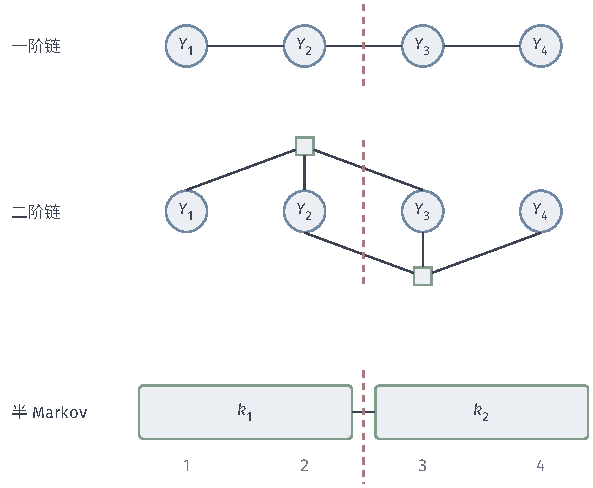
\includegraphics[width=100.404mm]{figures/06-probabilistic-graphical-models/04-models/tikz/pgm-energy-models-crf-scopes/figure.pdf}
  \caption{链、有限阶历史与片段的边界信息。一阶链在切分处保留一个标签，二阶链的跨界三元势需保留两个；半Markov模型则在片段边界汇总。图示$[1,2]$、$[3,4]$是一种候选分段，概率推断还要累加其他合法边界。}
  \label{fig:pgm-energy-models-crf-scopes}
\end{figure}

\paragraph{参数学习}
学习片段特征时还要计算它出现的边缘概率。令$B_b(k)$为边界$b$后、前标签固定为$k$的后缀权重和，取$B_T(k)=1$，按下一片段长度及标签反向汇总。前一片段标签$j$与当前区间$[a,b]$、标签$k$组成的连接，其边缘概率为
\[
  \frac{A_{a-1}(j)
           e^{g(a,b,j,k;\bm{x})}B_b(k)}
       {Z_{\bm{\theta}}(\bm{x})}.
\]
由这些边缘可计算长度、形状和转移特征的期望。完整边界及标签对应式~\eqref{eq:pgm-energy-models-semi-distribution}的直接对数似然；只有粗标签时，相容的未知分段还须在分子中求和。以最优分段替代求和会改成另一训练目标。

若$g_{\bm\theta}(a,b,j,k;\bm x)=\bm\theta^\top\bm G(a,b,j,k;\bm x)$，一条完整标注记录的梯度就是观测分段的特征和减去模型下的特征和期望。上面的连接边缘为每个候选片段提供概率权重，由此累加模型期望，再用梯度方法更新参数。完整标注、固定线性特征的负对数似然仍是凸目标；分子需要汇总未知分段时，一般失去这一保证。

\subsection{多状态链条件随机场}
\label{sec:pgm-dynamic-undirected-factorial-crf}

\paragraph{模型结构}
我们可能同时预测设备的故障类型与运行模式。先确定模式、再将单个预测结果交给故障分类器，会丢掉模式的不确定性，也使后续故障证据无法修正模式判断。\term{动态条件随机场}（dynamic conditional random field, DCRF）在每个时间片设置一组状态变量，并沿序列复用局部结构与参数。\term{因子条件随机场}（factorial CRF, FCRF）使用多条标签链，并增加同一时刻链间的相容关系，是一种代表构造\scite{pgm-dynamic-undirected-sutton2007}。

记第$r$条链的标签为$Y_t^{(r)}\in\{1,\ldots,K\}$，共有$R$条链，片内链间连接为$\mathcal E_c$。一种成对得分为
\begin{equation}
  \begin{aligned}
    F(\bm y;\bm x)={}&\sum_{t,r}a_t^{(r)}(y_t^{(r)};\bm x)
       +\sum_{t=2}^T\sum_r b_t^{(r)}
                (y_{t-1}^{(r)},y_t^{(r)};\bm x)\\
       &+\sum_t\sum_{(r,s)\in\mathcal E_c}
              c_t^{(r,s)}(y_t^{(r)},y_t^{(s)};\bm x).
  \end{aligned}
  \label{eq:pgm-dynamic-undirected-factorial-score}
\end{equation}
条件配分函数汇总全部标签链的联合配置。将片内耦合项去掉，且没有其他跨链作用时，分布才分解成各条独立CRF。因子HMM也组织多条状态链，但通常还为观测建立生成机制；FCRF直接评价给定输入后的标签组合，不需要给读数的相关特征规定联合分布。

\paragraph{推断}
合并$R$个标签得到$K^R$种切片状态，可以精确执行链递推；把转移当作稠密表时，基线成本为$O(TK^{2R})$。原来的因子结构可能允许更有效的消元，但片内与跨片关系组成的环不能直接当成$R$条互不影响的链。推断宽度可承受时使用团树；否则用变分或环消息等方法，并核对目标边缘。消息达到固定点不自动说明边缘正确，也不保证固定点总能达到。

\paragraph{参数学习}
所有标签都完整标注、得分对参数线性时，梯度仍是观测联合特征减去条件模型期望。不同之处在于后者需要耦合图的边缘，而非分别计算各链边缘。若只标注故障类型、没有模式标签，观测似然的分子也要对相容模式求和，数据端与模型端均需推断；不能把当前最可能模式当作完整标签而保持原目标。精确完整标签目标的凸性也不能直接迁移到这种部分标注目标。

\subsection{潜状态条件随机场}
\label{sec:pgm-dynamic-undirected-hidden-crf}

\paragraph{模型结构}
同一种故障可能经历升温、持续过热与恢复阶段，任务标签只写“故障”，没有标注这些内部阶段。多状态链允许同时描述多类状态，潜状态模型进一步把内部阶段视为未观测变量，训练时汇总其不确定性。需要先分清两种输出：给整段序列一个类别，或给每个位置一个标签。

整段类别记为$C\in\{1,\ldots,M\}$，内部状态为$H_t\in\{1,\ldots,K\}$。\term{隐状态条件随机场}（hidden-state CRF, HCRF）的一种链式构造对类别和潜状态共同评分，取
\begin{equation}
  \begin{aligned}
    F_{\bm\theta}(c,\bm h;\bm x)
      &=\eta_c+\sum_t a_{t,c}(h_t;\bm x)
                      +\sum_{t=2}^T b_{t,c}(h_{t-1},h_t;\bm x),\\
    p_{\bm\theta}(c\mid\bm x)
      &=\frac{\sum_{\bm h}\exp F_{\bm\theta}(c,\bm h;\bm x)}
        {\sum_{c'}\sum_{\bm h}\exp F_{\bm\theta}(c',\bm h;\bm x)}.
  \end{aligned}
  \label{eq:pgm-dynamic-undirected-hcrf}
\end{equation}
类别确定待比较的整体解释，潜状态链表达该类别内部的变化。同一类别的概率累加全部相容内部轨迹，不只评价最好的一条。它适合整段已经确定的分类单元，逐点分段还需另行规定输出\scite{pgm-dynamic-undirected-quattoni2007}。

逐点输出$Y_t\in\{1,\ldots,M\}$时，\term{潜动态条件随机场}（latent-dynamic CRF, LDCRF）可以为每个标签$k$指定互不相交的潜状态集合$\mathcal H_k$，全部潜状态组成$\mathcal H=\bigcup_k\mathcal H_k$。潜状态链$p_{\bm\theta}(\bm h\mid\bm x)$采用式~\eqref{eq:pgm-energy-models-chain-score}的单点与相邻得分，将状态空间改为$h_t\in\mathcal H$，并对全部潜状态轨迹归一化。再汇总与标签序列相容的潜状态：
\begin{equation}
  p_{\bm\theta}(\bm y\mid\bm x)
      =\sum_{\bm h:\,h_t\in\mathcal H_{y_t}\ \forall t}
                    p_{\bm\theta}(\bm h\mid\bm x).
  \label{eq:pgm-dynamic-undirected-ldcrf}
\end{equation}
每条潜状态轨迹唯一确定一条标签序列，所以这些事件不重叠，全部标签概率之和为$1$。同一标签集合内的状态切换表达内部阶段，不同集合之间的切换表达类别变化。这一构造同时保留逐点标签与标签内部的动态解释\scite{pgm-dynamic-undirected-morency2007}。

\paragraph{推断}
HCRF对每个类别执行一次潜状态链的前向求和，得到类别权重，再在类别之间归一化。每类$K$个状态、稠密转移下，$M$类查询需$O(MTK^2)$时间。以最大化替代内部求和会改变类别评分：一类有多条中等权重轨迹时，其总概率可能高于另一类的单条最佳轨迹。

LDCRF先计算潜状态边缘，再对集合$\mathcal H_k$求和，得到单位置标签概率。对一条已知标签序列求概率时，将不属于对应集合的状态势置零，前向求和给出相容轨迹权重，再除以不加限制的配分函数。逐点选最大标签边缘与选择概率最大的整段标签序列仍是不同查询；把最佳潜状态轨迹映射成标签，也未必得到后者。

\paragraph{参数学习}
两类模型的训练数据都不含内部状态标注。对线性得分$F_{\bm\theta}=\bm\theta^\top\bm G$，以$\bm O$表示任务输出变量，观测值记为$\bm o$，其似然梯度可写为
\begin{equation}
  \nabla_{\bm\theta}\log p_{\bm\theta}(\bm o\mid\bm x)
    =\mathbb E_{p_{\bm\theta}(\bm H\mid\bm o,\bm x)}
                        \bm G(\bm o,\bm H,\bm x)
      -\mathbb E_{p_{\bm\theta}(\bm O,\bm H\mid\bm x)}
                        \bm G(\bm O,\bm H,\bm x).
  \label{eq:pgm-dynamic-undirected-hidden-gradient}
\end{equation}
HCRF的$\bm o$是一个类别，LDCRF的$\bm o$是一条标签序列。第一项在已知输出下汇总潜状态，第二项汇总所有输出与潜状态；二者对应分子与分母的对数权重导数。对于LDCRF，输出由潜状态唯一决定，第二项可直接在潜状态链上计算。

负对数似然是两个对数求和指数项之差，通常不再凸。潜状态数量、初始化、正则化和局部最优都影响拟合，状态置换还可能保留同一观测分布。潜状态能够丰富标签内部的解释，但仅靠观测分类效果，无法把它们唯一命名为真实故障阶段。

\section{模型关系与比较}
\label{sec:pgm-dynamic-undirected-comparison}

先判断要评价什么分布。联合链和时空随机场为建模状态规定整段概率，可以补全状态或生成配置；条件模型固定读数，只比较可能的任务输出。动态有向模型通常把转移与观测生成分开，动态无向模型通过相容势组合关系，两者在有限链和高斯链中可能表示同一分布。因此，是否有箭头与是否给输入建立生成模型，是两个需要分别判断的选择。

若输出是逐点单标签，线性链CRF提供相邻关系和精确动态规划；需要更长的有限标签历史时，可增加消息记忆。若重点是区间长度、边界与内部形状，半Markov模型直接对片段评分。二者改变不同对象：前者扩大历史作用域，后者改变候选输出的单位，不能仅按名称中的“Markov”归为同一种改进。

多个输出任务彼此依赖时，FCRF保留同片与跨片耦合，避免把前一任务的单个预测当成确定证据；代价是更大的接口或近似推断。内部阶段没有标注时，HCRF和LDCRF在输出概率中汇总潜状态，分别面向整段类别与逐点标签。它们还可以与多状态或片段结构组合，代价要由组合后的图及查询重新分析。

计算比较应区分得分求值、概率归一化、边缘查询与最优输出。单状态离散链有有限状态递推，高斯链有解析矩计算，多变量时空或多标签图则可能需要更宽的消元或近似。隐状态链仍能精确求和，但含潜状态的最优标签查询不等于对全部变量取最大，参数训练也可能失去凸性。

训练和评价都应明确记录单位及可用观测。整段分类、逐点标签错误、完整标签序列错误和片段边界误差回答不同问题；在线预测也不能使用训练或测试时尚未到来的未来读数。按记录分离训练与评价并检查实际查询，比只报告训练目标是否下降更能说明所用模型的效果。

\section{本章小结}
\label{sec:pgm-dynamic-undirected-summary}

相邻时刻的状态可以通过相容权重联系起来，再对整段配置共同归一化。单点边缘相同的模型，仍可能对持续故障给出不同联合概率；三位置离散链说明了这一差别。时间先后不强迫局部权重具有生成方向，链式与高斯式分解也可以与有向表示对应。

模型选择首先取决于需要预测或生成的对象。联合链描述状态分布，时空耦合增加同片关系；条件链预测标签，半Markov模型增加边界与片段，FCRF协调多个输出，潜状态模型汇总未标注的内部解释。它们改变的对象可以组合，归一化与查询成本则需要随接口和因子作用域重新检查。

回到报警判断，若只需已知读数下的标签，可使用条件模型；若还需状态或读数的生成预测，就要明确联合建模的变量及观测机制。无论采用哪种表示，都应分别确认分布合法、所需查询可算、训练目标可求解，以及评价使用的信息是否符合任务。

\paragraph{延展阅读}
Sutton与McCallum的教程可用于复核线性链、条件似然和消息计算；Sarawagi与Cohen的半Markov工作展开片段输出。多状态依赖可继续读Sutton等人的动态条件随机场，潜状态输出可对照Quattoni等人的HCRF与Morency等人的LDCRF。连续链和稀疏时空推断则可接到Rue与Held的高斯随机场教材，重点比较查询对象及精度矩阵结构\scite{pgm-energy-models-sutton2012,pgm-energy-models-sarawagi2004,pgm-dynamic-undirected-sutton2007,pgm-dynamic-undirected-quattoni2007,pgm-dynamic-undirected-morency2007,pgm-undirected-rue2005}。

\chapter{概率生成模型}
\label{chap:pgm-generative}

前面几章的模型主要使用手工选定的简单分布（条件概率表、高斯、线性势），它们可解释、计算常常闭合，但难以直接刻画图像、语音这类维数高、结构复杂的数据。本章讨论怎样用神经网络定义足够灵活且在概率上合法的分布，使分布能够归一化、可以训练，也能采样新样本。主要困难在于，噪声到样本的网络映射本身不构成可计算概率模型；能够生成图片，并不意味着已知这些图片的密度，也就难以直接使用最大似然训练。

本章围绕如何给简单初始分布（通常是标准高斯噪声）逐步赋予复杂结构，讨论三种代表性构造。第一种是\emph{潜变量边缘化}（VAE）：保留多种潜在原因可产生同一观测的多对一关系，观测密度是对潜变量的积分，用变分下界处理不可解析的积分。第二种是\emph{可逆变换}（规范化流）：要求变换是一一对应的双射，因此无需对潜变量求和，只需按变量变换公式追踪每一步的体积伸缩就能精确计算密度。第三种是\emph{逐步去噪}（扩散模型）：人为设计把数据逐步加噪成纯噪声的过程，再学习每一小步的逆过程，将复杂样本生成拆成一系列去噪监督任务。三者能产生相似样本，却在密度可计算性、潜变量含义和采样成本上各有取舍。

生成模型既用于评价给定观测的概率，也用于生成新观测，这两项任务的计算代价可能相差很大。例如，从噪声到图像的网络可以迅速输出样本，而给定图像的密度可能难以求值；采用条件分解的模型可以精确评价完整观测的似然，生成时却可能需要逐个输出分量。图分解、边缘化和近似推断把这些差异落实为具体计算：先确定查询的概率对象，再找出其中未观测的变量，以及需要执行的求和、积分或变量变换。

本章考察三种构造复杂观测分布的机制：潜变量边缘化、可逆变量变换和人工随机过程。每种机制都需要说明分布为何归一化、训练目标如何联系似然，以及生成样本所需的计算。神经网络分别参数化条件分布、可逆映射或局部转移；这些概率角色决定了模型的表达限制、学习误差和查询成本。

\section{复杂观测的概率建模问题}

\label{sec:pgm-generative-common}

本节固定全章共同的概率语言：为数据建立生成分布的含义、最大似然训练的计算对象，以及只能采样而不能求密度的边界情形（如GAN）。设训练样本$\bm{x}_1,\ldots,\bm{x}_n$独立同分布地来自未知分布$p_{\mathrm{data}}$，用参数向量$\bm{\theta}$确定的$p_{\bm{\theta}}$近似数据分布。除特别说明外，观测取值于$\mathbb{R}^{d}$，本章用连续密度描述它们：区域上的概率由密度积分得到，单点密度值可以大于$1$。二值或离散观测则用概率质量函数描述，各个取值的质量直接表示其概率。比较模型似然时，各模型需采用相同的观测表示和测度。

\term{概率生成模型}（probabilistic generative model）为可能出现的观测规定一个分布，并据此生成新观测。对显式密度模型，归一化要求$\int p_{\bm{\theta}}(\bm{x})\,\mathrm{d}\bm{x}=1$。最大似然学习最小化
\begin{equation}
  \label{eq:pgm-generative-nll}
  J(\bm{\theta})
  =-\frac{1}{n}\sum_{i=1}^{n}\log p_{\bm{\theta}}(\bm{x}_i).
\end{equation}
计算该目标需要评价每个观测的对数密度。潜变量模型中的积分可能成为主要障碍；只给出噪声到观测的生成程序时，还需要确认观测密度是否存在，以及如何求值。因此，模型的训练规则、密度评价、采样步骤和潜变量推断各有独立的计算要求。

自回归模型用归一化的一维条件分布按链式法则构成联合分布。给定完整观测后，各条件分布可以直接评价；祖先采样则通常按照分解顺序生成各分量（见第~\ref{sec:pgm-static-directed-autoregressive}节）。以此为基线，下面考察三种计算安排：VAE通过潜变量积分定义观测密度，规范化流用双射的体积变化追踪密度，扩散模型通过多次局部随机转移生成观测。

三种机制使用的概率结构有所不同。VAE采用有向潜变量图；离散扩散采用沿人工噪声索引展开的有向Markov链；规范化流依靠确定性双射和变量变换公式，其计算图记录变换依赖，条件独立性仍需由相应概率模型确定。后文还将介绍概率电路：它通过约束计算图的结构支持精确边缘化和条件查询，补充上述三种机制在查询方面的取舍。

本章用一维目标$X\sim\mathcal{N}(0,5)$贯穿三种机制。独立高斯变量相加、标准高斯缩放和以该分布为起点的前向扩散，分别提供可解析的例子。相同的观测分布使比较集中于潜变量含义、密度计算和随机路径，而复杂数据的表达限制将在各机制中另行讨论。

\paragraph{生成程序与密度评价}
\label{sec:pgm-generative-implicit-boundary}

假设只给出$\bm{Z}\sim p_0$和生成程序$\bm{X}=G_{\bm{\theta}}(\bm{Z})$。对任意可测集合$B$，它已经规定
\begin{equation}
  \label{eq:pgm-generative-pushforward}
  \mathbb{P}_{\bm{\theta}}(\bm{X}\in B)
  =\int \mathbf{1}\{G_{\bm{\theta}}(\bm{z})\in B\}
           p_0(\bm{z})\,\mathrm{d}\bm{z}.
\end{equation}
这种通过采样程序间接规定的分布称为\term{隐式分布}（implicit distribution）。\term{生成对抗网络}（generative adversarial network, GAN）是常见例子：通常的生成器提供样本，却不提供通过变量变换直接评价的观测密度。这里将GAN作为通过生成程序定义分布的例子，相关比较针对密度与采样查询；网络结构与对抗学习见\BookChapterRef{chap:neural-generative-models}{神经网络模型部分的“基于神经网络的生成模型”章}\scite{pgm-generative-goodfellow2014}

密度评价涉及逆像计算，也涉及采用的测度。同维光滑映射即使处处局部可逆，全局多对一时通常仍需累加所有逆像的贡献，普通网络未必支持枚举这些逆像。若基础变量维度低于观测维度，局部Lipschitz生成网络的输出还可能集中于低维集合，在整个观测空间的Lebesgue测度下没有密度。推送公式依然定义合法分布，相应查询需要采用适合该分布的概率表达。

\section{基于潜变量边缘化的分布构造}

\label{sec:pgm-generative-vae}

多个潜在解释可对同一观测作出贡献，观测密度因此是对这些解释的积分。为同时保留灵活的生成分布和可执行的参数学习，下面先建立生成结构，再把边缘积分转成可估计的下界；随后分别讨论推断误差、增加随机层次和加入已知生成条件所改变的对象。

\subsection{生成结构与观测分布}

\label{sec:pgm-generative-latent-model}

潜变量模型的基本想法在第11、13章已反复出现：观测到的复杂现象背后有少数未观测因素在起作用，把这些因素积分掉就得到观测分布。当时用线性高斯等简单形式，积分还能解析完成；一旦把条件分布换成强力的神经网络来刻画“给定潜变量、观测长什么样”，这个积分通常就再也积不出来，而后验$p(\bm z\mid\bm x)$也不再是简单高斯。VAE的贡献正是为这种\emph{非线性}潜变量模型配一套可训练的方案：用一个额外的网络近似后验，再用变分下界（第7章）把难算的积分变成可优化的目标。潜变量模型用未观测因素解释观测中共同变化的部分：先抽取潜变量，再按给定潜变量的条件分布生成观测。将条件分布的均值等参数交给非线性网络，可以描述更复杂的观测关系，但观测似然仍要对潜变量积分。在这种非线性模型中，后验通常无法像线性高斯模型那样解析求出，训练所需的后验计算也随之变难。一个办法是沿用第~\ref{chap:pgm-variational}章的分布近似，再学习一个从观测直接输出近似参数的共享映射，使训练样本和新样本都能复用它。\term{变分自编码器}（variational autoencoder, VAE）为这一生成模型配备可学习的近似后验。生成网络参数化条件分布，推断网络根据观测给出潜变量的近似分布；两者通过变分目标共同训练\scite{kingma2013}

令$\bm{z}\in\mathbb{R}^{k}$，通常取先验$p(\bm{z})=\mathcal{N}(\bm{0},\bm{I}_k)$，再用神经网络输出条件分布$p_{\bm{\theta}}(\bm{x}\mid\bm{z})$的参数。生成联合分布与观测边缘分布为
\begin{equation}
  \label{eq:pgm-generative-vae-joint}
  \begin{aligned}
    p_{\bm{\theta}}(\bm{x},\bm{z})
      &=p(\bm{z})p_{\bm{\theta}}(\bm{x}\mid\bm{z}),\\
    p_{\bm{\theta}}(\bm{x})
      &=\int p(\bm{z})p_{\bm{\theta}}(\bm{x}\mid\bm{z})
          \,\mathrm{d}\bm{z}.
  \end{aligned}
\end{equation}
先验和每个条件分布归一化时，交换非负积分的次序即可证明观测分布归一化。评价某个观测的似然仍需要计算式中的潜变量积分，其难度取决于条件分布的形式和潜变量维数。

对于连续观测，\term{解码器}（decoder）输出给定潜变量时观测分布的参数。常用的各向同性高斯设定为
\begin{equation}
  \label{eq:pgm-generative-gaussian-decoder}
  p_{\bm{\theta}}(\bm{x}\mid\bm{z})
  =\mathcal{N}\bigl(\bm{x};
    \bm{g}_{\bm{\theta}}(\bm{z}),\tau^2\bm{I}_d\bigr),
  \qquad \tau>0.
\end{equation}
其中$\bm{g}_{\bm{\theta}}:\mathbb{R}^{k}\to\mathbb{R}^{d}$给出条件均值，$\tau^2$为条件噪声方差。一次完整生成先抽取$\bm{z}\sim p$，再抽取独立标准高斯噪声$\bm{\eta}$，得到$\bm{x}=\bm{g}_{\bm{\theta}}(\bm{z})+\tau\bm{\eta}$。实际展示也可能只输出条件均值$\bm{g}_{\bm{\theta}}(\bm{z})$；这会省去观测噪声，与式~\eqref{eq:pgm-generative-gaussian-decoder}规定的随机采样对应不同输出。

线性解码器$\bm{g}_{\bm{\theta}}(\bm{z})=\bm{W}\bm{z}+\bm{b}$与独立高斯噪声共同构成线性高斯模型，其中$\bm{W}\in\mathbb{R}^{d\times k}$。将潜变量变换的协方差与噪声协方差相加，得到观测边缘分布（见第~\ref{sec:pgm-static-directed-linear-gaussian}节）：
\[
  p_{\bm{\theta}}(\bm{x})
  =\mathcal{N}\bigl(\bm{x};
    \bm{b},\bm{W}\bm{W}^{\top}+\tau^2\bm{I}_d\bigr).
\]

潜变量后验可以通过配平方求得。对数联合分布中，先验和观测似然的二次项相加，给出后验精度矩阵$\bm{I}_k+\tau^{-2}\bm{W}^{\top}\bm{W}$；线性项进一步确定后验均值：
\begin{equation}
  \label{eq:pgm-generative-linear-posterior}
  \begin{aligned}
    \bm{\Sigma}
      &=\bigl(\bm{I}_k+\tau^{-2}\bm{W}^{\top}\bm{W}\bigr)^{-1},\\
    \bm{m}(\bm{x})
      &=\tau^{-2}\bm{\Sigma}\bm{W}^{\top}(\bm{x}-\bm{b}),\\
    p_{\bm{\theta}}(\bm{z}\mid\bm{x})
      &=\mathcal{N}\bigl(\bm{z};\bm{m}(\bm{x}),\bm{\Sigma}\bigr).
  \end{aligned}
\end{equation}

非线性解码器可以表达弯曲、非高斯的观测分布。此时，$\lVert\bm{x}-\bm{g}_{\bm{\theta}}(\bm{z})\rVert_2^2$通常不再是潜变量的二次式，前述配平方计算便失去适用条件，边缘密度和后验一般需要近似求解。VAE保留式~\eqref{eq:pgm-generative-vae-joint}的生成定义，用近似后验支持参数学习。

\begin{example}[同一观测分布的潜变量解释]
  \label{ex:pgm-generative-gaussian-latent}
  取$Z\sim\mathcal{N}(0,1)$、$E\sim\mathcal{N}(0,1)$且二者独立，令$X=2Z+E$，于是$X\sim\mathcal{N}(0,5)$。观测$x=2$后，
  \[
    p(z\mid x=2)\propto
    \exp\left[-\frac{1}{2}\{z^2+(2-2z)^2\}\right]
    \propto\exp\left[-\frac{5}{2}(z-0.8)^2\right].
  \]
  后验为$\mathcal{N}(0.8,0.2)$。独立观测噪声使多个潜变量取值都可以解释$x=2$，因此给定观测后仍保留潜变量不确定性。后文的Flow则为完整观测规定唯一逆像。
\end{example}

\subsection{ELBO目标与重参数化学习}


\label{sec:pgm-generative-vae-objective}

观测边缘积分难以求值时，可以用近似后验构造证据下界。将式~\eqref{eq:pgm-generative-vae-joint}的联合分解代入一般ELBO，得到条件对数似然的期望减去近似后验与先验的KL散度（见式~\eqref{eq:pgm-variational-elbo}）：
\begin{equation}
  \label{eq:pgm-generative-vae-elbo}
  \begin{aligned}
    \mathcal{L}(\bm{\theta},\bm{\phi};\bm{x})
    ={}&\mathbb{E}_{q_{\bm{\phi}}(\bm{z}\mid\bm{x})}
       [\log p_{\bm{\theta}}(\bm{x}\mid\bm{z})]\\
      &-\operatorname{KL}\bigl(
       q_{\bm{\phi}}(\bm{z}\mid\bm{x})\,\|\,p(\bm{z})\bigr)
      \leq\log p_{\bm{\theta}}(\bm{x}).
  \end{aligned}
\end{equation}

\term{编码器}（encoder）根据观测输出$q_{\bm{\phi}}(\bm{z}\mid\bm{x})$的分布参数。同一组权重$\bm{\phi}$在不同观测之间共享，均值和尺度随输入变化；这构成摊销推断，$\bm{\phi}$对应第~\ref{sec:pgm-variational-amortized}节的$\bm{\omega}$。生成参数$\bm{\theta}$属于观测条件分布。图~\ref{fig:pgm-generative-vae}分别表示两套计算：先验与解码器规定生成联合分布，编码器在训练和观测后推断时提供近似后验。

ELBO中的期望是对$q_{\bm\phi}(\bm z\mid\bm x)$求的，训练时要从这个分布抽样$\bm z$，但抽样操作本身不可导，梯度无法从解码器穿过随机抽样回传给编码器。重参数化技巧把\emph{随机性的来源}和\emph{含参数的确定性变换}分开：不直接从$\mathcal N(m,s^2)$抽$\bm z$，而是先从与参数无关的标准高斯抽$\bm\epsilon$，再令$\bm z=\bm m+\bm s\odot\bm\epsilon$。这样随机性移到不含参数的$\bm\epsilon$上，梯度可沿$m,s$和解码器这条确定路径反传。为让重构期望中的抽样参与梯度计算，图中把近似后验样本表示成独立噪声的可微变换，变换参数由编码器给出。下面以对角高斯说明具体计算。

对有限训练集，VAE实际联合优化生成参数$\bm\theta$与编码器参数$\bm\phi$。在先验固定的设定下，其经验目标函数为
\begin{equation}
  \label{eq:pgm-generative-vae-empirical-objective}
  \min_{\bm\theta,\bm\phi}\;
  J_{\mathrm{VAE}}(\bm\theta,\bm\phi)
  =-\frac1n\sum_{i=1}^{n}
       \mathcal L(\bm\theta,\bm\phi;\bm x_i).
\end{equation}
这仍是对数边缘似然的下界优化：生成网络改变被拟合的分布，编码器改变计算该下界所用的近似后验。两套参数通过同一个重构期望相互联系，不能把编码器的重构映射单独当作完整生成模型。下面将下界的两个部分化为可执行的训练计算。

\begin{figure}[htbp]
  \centering
  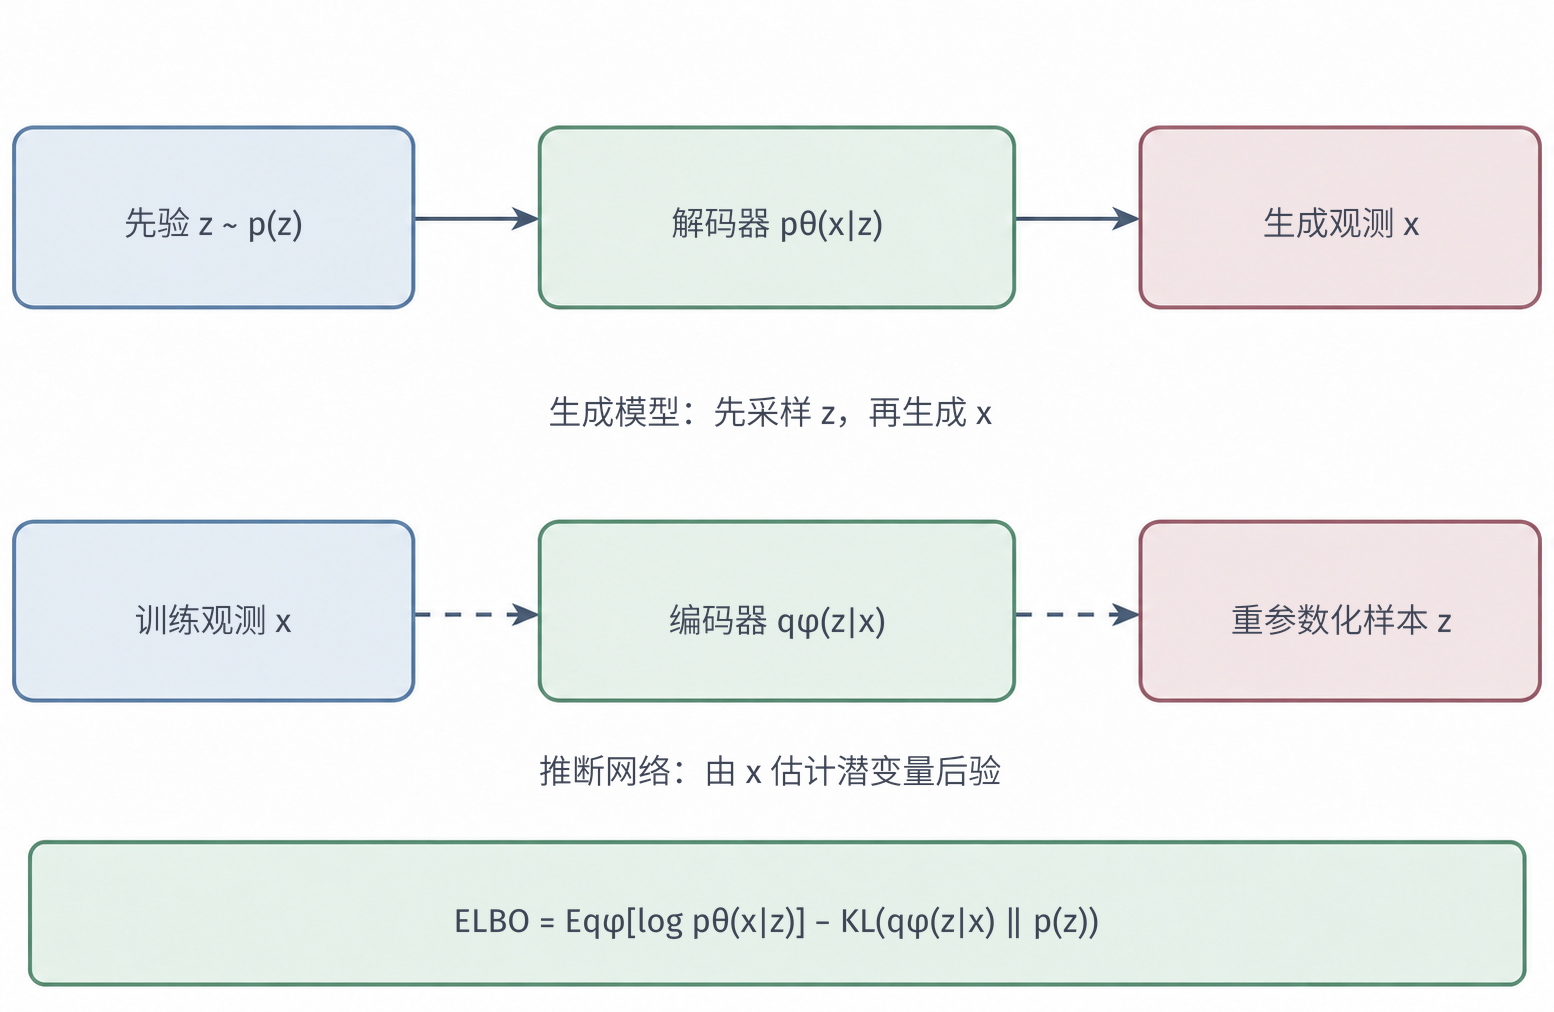
\includegraphics[width=112.000mm]{figures/06-probabilistic-graphical-models/04-models/generated/pgm-generative-vae/figure.png}
  \caption{VAE的生成与近似推断。上行实线表示从先验抽潜变量，再按$p_{\bm\theta}(\bm x\mid\bm z)$抽观测；下行虚线表示由观测构造$q_{\bm\phi}(\bm z\mid\bm x)$。两行分别记录生成分布和推断程序，底部ELBO联系条件似然与近似后验。}
  \label{fig:pgm-generative-vae}
\end{figure}

常用编码器取对角高斯
\[
  q_{\bm{\phi}}(\bm{z}\mid\bm{x})
  =\mathcal{N}\!\left(
    \bm{z};\bm{m}_{\bm{\phi}}(\bm{x}),
    \operatorname{diag}\bigl(\bm{s}_{\bm{\phi}}^2(\bm{x})\bigr)
    \right),
\]
其中每个$s_{\bm{\phi},j}(\bm{x})>0$。网络可以输出对数方差，再经指数变换得到正方差。对标准高斯先验，KL项解析可得：
\begin{equation}
  \label{eq:pgm-generative-diagonal-kl}
  \operatorname{KL}(q_{\bm{\phi}}\,\|\,p)
  =\frac{1}{2}\sum_{j=1}^{k}
     \bigl(m_{\bm{\phi},j}^2+s_{\bm{\phi},j}^2
            -1-\log s_{\bm{\phi},j}^2\bigr).
\end{equation}

式中省略了各分量对观测的依赖。为估计重构期望，抽取独立标准高斯噪声$\bm{\epsilon}$，经$\bm{z}=\bm{m}_{\bm{\phi}}(\bm{x})+\bm{s}_{\bm{\phi}}(\bm{x})\odot\bm{\epsilon}$得到后验样本，其中$\odot$表示逐元素乘法。噪声分布与网络参数无关，样本梯度可沿均值、尺度和解码器组成的可微路径计算。要让样本梯度的期望等于目标梯度，即给出无偏估计，还需交换参数微分与期望；例如，在参数邻域内可微且相应导数受可积函数控制。若还要求估计方差有限，则另需梯度二阶矩有限（见第~\ref{chap:pgm-variational}章）。一次编码器前向计算给出当前观测的近似后验参数，省去了逐样本优化变分参数的步骤。

图~\ref{fig:vae-reparameterization-training}表示重参数化后的训练路径：独立噪声经编码器给出的均值与尺度变换为潜变量，重构项的梯度再通过解码器传回编码器。无条件生成采用先验样本进入解码器。

\begin{figure*}[htbp]
  \centering
  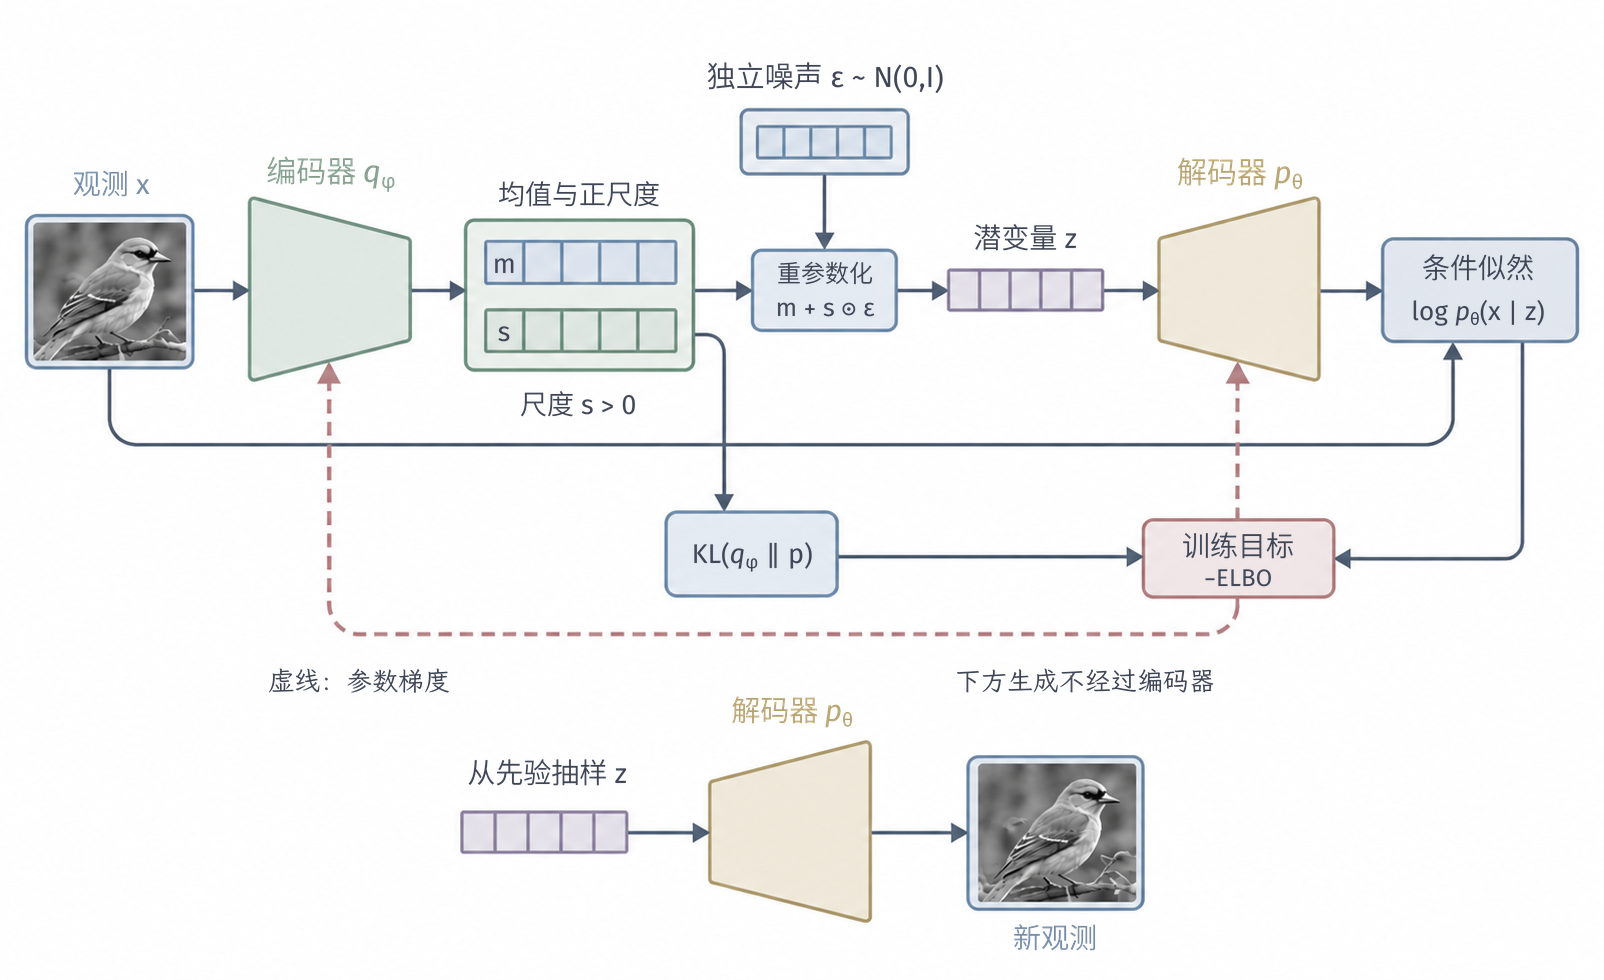
\includegraphics[width=135.805mm]{figures/06-probabilistic-graphical-models/04-models/generated/vae-reparameterization-training/figure.png}
  \caption{对角高斯VAE的重参数化与训练。编码器给出均值$\bm m$和正尺度$\bm s$，独立标准正态噪声经$\bm z=\bm m+\bm s\odot\bm\epsilon$形成潜变量，并进入解码器规定的条件分布。重构对数似然的期望与KL项组成ELBO，图中的负ELBO框表示训练目标。生成阶段从先验抽样，不经过编码器；鸟图为概念插画。}
  \label{fig:vae-reparameterization-training}
\end{figure*}

ELBO中的重构项由观测条件分布确定。对于式~\eqref{eq:pgm-generative-gaussian-decoder}的高斯解码器，负对数似然分解为加权平方误差和方差相关项：
\begin{equation}
  \label{eq:pgm-generative-reconstruction}
  -\log p_{\bm{\theta}}(\bm{x}\mid\bm{z})
  =\frac{\lVert\bm{x}-\bm{g}_{\bm{\theta}}(\bm{z})\rVert_2^2}
          {2\tau^2}
    +\frac{d}{2}\log(2\pi\tau^2).
\end{equation}
固定$\tau$时，最后一项与待学习参数无关。若方差参与学习，对数方差项与平方误差权重共同约束它：增大方差会减轻平方误差的代价，同时提高对数方差代价。删去后一项会改变优化目标。对于二值观测$x_j\in\{0,1\}$，采用给定潜变量后独立的Bernoulli分布，解码器输出参数$\pi_j(\bm{z})$，负对数似然为
\[
  -\sum_{j=1}^{d}
    \bigl[x_j\log\pi_j(\bm{z})
      +(1-x_j)\log(1-\pi_j(\bm{z}))\bigr].
\]

二值交叉熵由此来自Bernoulli观测假设。连续灰度值具有不同的取值空间；对它使用相同表达式时，需说明作为代理损失的含义。离散像素可以采用类别质量函数，也可以将连续条件密度在相应量化区间内积分得到概率质量。

在例~\ref{ex:pgm-generative-gaussian-latent}中，让编码器恰好输出$q(z\mid2)=\mathcal{N}(0.8,0.2)$，可以逐项复核ELBO：
\[
  \begin{aligned}
    \mathbb{E}_{q}(2-2Z)^2&=(2-1.6)^2+4(0.2)=0.96,\\
    \mathbb{E}_{q}\log p(2\mid Z)&=-\tfrac12\log(2\pi)-0.48,\\
    \operatorname{KL}(q\,\|\,p)&=
       \tfrac12\bigl(0.8^2+0.2-1-\log0.2\bigr).
  \end{aligned}
\]
各项相加得到$\mathcal{L}\approx-2.12366$，等于观测对数密度：
\[
  \log\mathcal{N}(2;0,5)
  =-\tfrac12\log(10\pi)-0.4.
\]
将近似后验改为先验时，ELBO降为$-\tfrac12\log(2\pi)-4\approx-4.91894$。两次计算使用相同生成模型，下界差异由近似后验与真实后验的匹配程度引起。

训练时，对小批量观测运行编码器，抽取标准噪声并计算ELBO的随机估计，再更新生成参数和共享编码器参数。停止条件可由计算预算或验证指标确定。设一次编码和解码的代价分别为$C_{\mathrm{enc}}$和$C_{\mathrm{dec}}$；每个观测使用一个潜变量样本时，前向代价约为$O(C_{\mathrm{enc}}+C_{\mathrm{dec}}+k)$，反向传播通常为同阶。增加后验样本可降低部分蒙特卡洛方差，同时增加解码计算。无条件生成只需先验采样和解码；观测后的近似推断只需一次编码器计算。

\subsection{推断误差、潜变量利用与表达限制}
\label{sec:pgm-generative-vae-failure}

VAE用下界替代真实似然，其误差需要分层定位，共有三个互不相同的来源：一是生成模型这个\emph{候选分布族}本身表达力不够；二是即便固定生成模型，我们允许近似后验取的\emph{分布族}（如对角高斯）形状受限；三是用\emph{同一个编码器网络}去对所有样本输出后验参数，未必能对每个样本都给出该族下的最优后验（这是“摊销”带来的代价）。VAE的误差来自生成分布、近似后验和共享编码器三个层次。\term{模型近似误差}（model approximation error）由候选$p_{\bm{\theta}}$与数据分布的差距产生，需通过调整生成族处理。固定生成参数后，近似后验族的形状限制产生\term{近似族误差}（variational approximation error）。逐个观测的最优变分参数若无法由同一编码器同时表示，还会产生\term{摊销误差}（amortization error）。设$\mathcal{Q}$为候选后验族，$\mathcal{L}_{\mathcal{Q}}^*(\bm{x})=\sup_{q\in\mathcal{Q}}\mathcal{L}(\bm{\theta},q;\bm{x})$为固定模型下该族的最优下界，且$q_{\bm{\phi}}(\cdot\mid\bm{x})\in\mathcal{Q}$。下界差距可分解为
\begin{equation}
  \label{eq:pgm-generative-inference-gaps}
  \begin{aligned}
    \log p_{\bm{\theta}}(\bm{x})
      -\mathcal{L}(\bm{\theta},\bm{\phi};\bm{x})
    ={}&\bigl[\log p_{\bm{\theta}}(\bm{x})
             -\mathcal{L}_{\mathcal{Q}}^*(\bm{x})\bigr]\\
       &+\bigl[\mathcal{L}_{\mathcal{Q}}^*(\bm{x})
             -\mathcal{L}(\bm{\theta},\bm{\phi};\bm{x})\bigr].
  \end{aligned}
\end{equation}

第一项为近似族误差，第二项为当前编码器相对于逐观测最优解的差距，两项均非负。第二项还包含编码器优化不足；进一步比较最优共享编码器，可以区分摊销限制与优化误差（见式~\eqref{eq:pgm-variational-amortization-gap}）。增加生成族容量、扩大后验族和改进编码器优化，分别针对这些不同来源的误差。

\paragraph{潜变量利用与后验坍塌}

训练VAE时还会遇到一个典型病态：潜变量似乎“白设了”——编码器对任何输入输出的后验都几乎等于先验，解码器干脆忽略潜变量、退化成一个不依赖$\bm z$的独立模型。这通常发生在解码器过强、不靠潜变量也能拟合数据时：此时使用潜变量带来的重构收益抵不过KL惩罚，优化就停在“后验＝先验”的状态。编码器还可能几乎不携带观测信息。近似后验接近先验的现象称为\term{后验坍塌}（posterior collapse），即$q_{\bm{\phi}}(\bm{z}\mid\bm{x})\approx p(\bm{z})$；部分坐标也可以单独出现这种现象。该定义针对近似后验，真实后验需由生成模型另行判断。以例~\ref{ex:pgm-generative-gaussian-latent}为例，编码器总输出先验时，生成模型在$x=2$处的真实后验仍为$\mathcal{N}(0.8,0.2)$，两者的差异表现为推断误差。

若解码器忽略全部潜变量，即$p_{\bm{\theta}}(\bm{x}\mid\bm{z})=p_{\bm{\theta}}(\bm{x})$，真实后验便等于先验。固定这一生成模型时，近似后验取先验即可使ELBO达到最大。表达力强的解码器可能在利用潜变量之前就充分拟合数据，此时利用潜变量所得的重构收益未必补偿KL代价，训练也可能停留在这一状态。编码器KL接近零因而提供了坍塌线索；判断真实潜变量依赖还需考察解码分布。解码器本身的生成质量则是另一项评价。

编码器在训练数据上产生的潜变量分布，可能与无条件生成采用的先验分布不同。定义\term{聚合后验}（aggregated posterior）
\begin{equation}
  \label{eq:pgm-generative-aggregated-posterior}
  q_{\mathrm{agg}}(\bm{z})
  =\mathbb{E}_{\bm{X}\sim p_{\mathrm{data}}}
       [q_{\bm{\phi}}(\bm{z}\mid\bm{X})],
\end{equation}
即把不同观测的编码分布按数据频率混合。假设相关KL有限，在$\log(q_{\bm{\phi}}/p)$中加减$\log q_{\mathrm{agg}}$，可得
\begin{equation}
  \label{eq:pgm-generative-kl-information}
  \mathbb{E}_{p_{\mathrm{data}}}
    \operatorname{KL}(q_{\bm{\phi}}(\bm{z}\mid\bm{X})\,\|\,p(\bm{z}))
  =I_q(\bm{X};\bm{Z})+
    \operatorname{KL}(q_{\mathrm{agg}}\,\|\,p).
\end{equation}
其中$I_q$是联合分布$p_{\mathrm{data}}(\bm{x})q_{\bm{\phi}}(\bm{z}\mid\bm{x})$下的互信息。逐样本KL同时约束编码中的数据信息和聚合后验与先验的匹配。有限训练后，先验仍可能在编码器很少访问的区域保留明显质量；无条件生成进入这些区域时，解码器的表现会受到训练支持不足的影响。

不同修正分别改变训练路径、生成结构或推断族。将KL系数从小值逐渐提高到$1$，可以调整训练中重构与先验匹配的相对作用；最终保持$\lambda\ne1$时，$\mathbb{E}_q\log p_{\bm{\theta}}(\bm{x}\mid\bm{z})-\lambda \operatorname{KL}(q\,\|\,p)$则成为不同于原ELBO的目标。$\lambda\geq1$时该目标仍不大于原ELBO，$\lambda<1$时缺少相同的下界保证。限制解码器绕过潜变量的信息通路会改变模型结构，扩大后验族主要减小推断差距，学习可评价密度的先验会改变生成模型和KL的比较对象。修正是否改善潜变量利用，需结合这些对象及实际优化结果判断。

\label{sec:pgm-generative-vae-expression}

\paragraph{观测分布与潜变量维度}

潜变量维度决定生成模型可以用多少自由度解释观测变化。即使$k<d$，式~\eqref{eq:pgm-generative-gaussian-decoder}中正方差噪声仍覆盖全部观测维度，使模型具有$d$维密度。去掉噪声后，光滑低维解码器的输出通常集中于低维集合。增大潜变量维度可减轻表示瓶颈，同时增加学习和推断的自由度；这些维度能否承载有效信息，还取决于训练目标与解码器对潜变量的利用。

给定潜变量后若仍存在多种不同观测，固定方差的单一高斯条件似然通过平方误差拟合它们的均值。在有限二阶矩条件下，允许所有只依赖该潜变量的二阶可积预测时，逐坐标的总体最优预测为$\mathbb E[\bm X\mid\bm z]$。这一结论说明平方重构为何趋向条件平均，可参考\BookChapterRef{chap:random-variables}{卷2《数学准备：概率、因果与决策》的“随机变量与概率基础”章}。例如，边缘等概率出现在左右两处时，均值图像会在两处留下较淡的边缘，这提供了模糊重构的一种解释。表达力更强的条件似然可以分别描述这些结果；在简单高斯均值上增加独立噪声，主要改变随机波动，恢复结构仍需相应条件分布。

\subsection{层次VAE与多层潜在解释}
\label{sec:pgm-generative-hierarchical-vae}

\paragraph{潜变量的层次表示}

标准VAE只设一层潜变量、且先验固定为标准高斯，这等于假设所有高层结构都要由解码器一个网络从无结构的高斯噪声里凭空造出来。让潜在因素本身也\emph{分层}——上层因素决定下层因素的分布——可以把“从整体结构到细节”的层级关系显式交给生成模型，积分掉上层后下层的边缘先验也不再局限于简单高斯。增加随机层次的动机是让一组潜在因素本身具有可学习的分布，而不是在一个固定高斯先验中承受全部结构。简单的想法是先抽上层因素，再由它决定下层因素的条件分布；把上层因素积分掉后，下层因素的边缘分布就可以超出原先固定标准高斯的形状。

\term{层次VAE}（hierarchical VAE）通过多层随机潜变量表示依赖，例如$p(\bm{z}_2)p_{\bm{\theta}}(\bm{z}_1\mid\bm{z}_2)p_{\bm{\theta}}(\bm{x}\mid\bm{z}_1)$。每一层都规定条件分布，因此同时增加生成模型的随机依赖和后验耦合；确定性解码网络的层数则属于条件分布内部的参数化。

近似后验也需要同时描述两层潜变量。可以先由观测推断下层因素，再结合它与观测推断上层因素。对于前文的两层例子，若取$q_{\bm{\phi}}(\bm{z}_1,\bm{z}_2\mid\bm{x})=q_{\bm{\phi}}(\bm{z}_1\mid\bm{x})q_{\bm{\phi}}(\bm{z}_2\mid\bm{z}_1,\bm{x})$，ELBO就是
\[
  \mathbb{E}_{q_{\bm{\phi}}}
  \left[
    \log\frac{
      p(\bm{z}_2)p_{\bm{\theta}}(\bm{z}_1\mid\bm{z}_2)
          p_{\bm{\theta}}(\bm{x}\mid\bm{z}_1)}
      {q_{\bm{\phi}}(\bm{z}_1\mid\bm{x})
          q_{\bm{\phi}}(\bm{z}_2\mid\bm{z}_1,\bm{x})}
  \right].
\]
下界继续采用生成联合与变分路径密度比的期望，可通过逐层抽样估计。每层后验都需与相应生成依赖匹配，层次模型因而仍存在推断误差和潜变量利用问题。

训练时，编码器依次给出两层近似条件分布的参数，逐层抽取样本并评价上式的生成项和推断项，再对所有生成参数与编码器参数更新负平均ELBO。可重参数化的连续条件分布允许沿各层计算路径求梯度；不满足这一条件的随机层需改用相应的梯度估计。生成时反过来按$\bm z_2\to\bm z_1\to\bm x$抽样。多层随机状态改变后验依赖和计算，而多层确定性网络只改变某个条件分布的函数形式。

\subsection{条件VAE与剩余随机性}

\label{sec:pgm-generative-vae-conditional}

普通VAE只能\emph{无条件}地随机生成，没法控制“我要一张某类设备的图”。要让生成可指定类别或属性，只需把这个已知条件$\bm m c$同时喂给先验、解码器和后验；潜变量则负责表达“在同一条件下样本之间仍有的差异”。无条件生成无法指定希望得到的类别或属性。若标签、文本属性或其他条件已知，生成目标可以改为在这些条件下描述观测的分布，潜变量则保留同一条件下仍可能出现的变化。

给定标签或其他条件$\bm{c}$时，\term{条件VAE}（conditional VAE）使用条件先验与条件解码分布$p_{\bm{\theta}}(\bm{z}\mid\bm{c})p_{\bm{\theta}}(\bm{x}\mid\bm{z},\bm{c})$，并用$q_{\bm{\phi}}(\bm{z}\mid\bm{x},\bm{c})$近似后验。潜变量可用于表示已知条件之外的剩余变化。

生成时固定$\bm c$，先从条件先验抽取潜变量，再按条件解码分布生成观测；训练时将同一条件同时提供给生成模型和近似后验。将条件联合分布与条件近似后验代入ELBO，即可得到$\log p_{\bm\theta}(\bm x\mid\bm c)$的下界。这里改变的是生成所依据的信息，条件并不消除潜变量积分或后验近似误差。

把每条训练记录写成$(\bm x_i,\bm c_i)$，条件模型的本地学习目标为
\begin{equation}
  \label{eq:pgm-generative-conditional-vae-objective}
  \begin{aligned}
    \min_{\bm\theta,\bm\phi}\; -\frac1n\sum_i
      \bigl\{&\mathbb E_{q_{\bm\phi}(\bm z\mid\bm x_i,\bm c_i)}
        \log p_{\bm\theta}(\bm x_i\mid\bm z,\bm c_i)\\
       &-\operatorname{KL}\bigl(q_{\bm\phi}(\bm z\mid\bm x_i,\bm c_i)
                   \,\|\,p_{\bm\theta}(\bm z\mid\bm c_i)\bigr)\bigr\}.
  \end{aligned}
\end{equation}
固定条件后，近似后验仍解释当前观测的剩余变化；条件先验则规定尚未看到观测时怎样生成这种变化。小批量训练把同一$\bm c_i$送入相应网络，抽取潜变量后计算重构项与KL项，再更新出现于目标中的参数；先验若也含可学习参数，它们同样接受更新。条件没有替我们选择唯一观测，所以生成阶段仍需要潜变量抽样以及条件解码。

\section{基于可逆变换的分布构造}

\label{sec:pgm-generative-flows}

\label{sec:pgm-generative-flow-structure}

VAE里多个潜变量取值都能解释同一观测，密度要靠\emph{积分}（实际用下界近似）。规范化流换了一个思路：干脆让基础噪声与观测\emph{一一对应}、变换完全可逆，于是任何观测都能唯一反推出那个噪声；这样根本不需要积分，只要用微积分里的“变量变换公式”补上变换造成的\emph{局部体积伸缩}（Jacobian行列式），就能得到精确密度。代价是必须精心设计网络，使它既可逆、行列式又好算。潜变量积分把多种可能原因汇成同一观测密度。现在保留同维基础噪声，却要求完整观测能够唯一恢复它；密度计算于是从积分变为局部体积换算。不同Flow结构共同回答怎样让逆变换和体积因子可算，区别主要落在坐标依赖及计算方向。

\subsection{变量变换与最大似然学习}
\label{sec:pgm-generative-flow-learning}

\label{sec:pgm-generative-change-of-variables}

多个潜变量及观测噪声可以产生同一观测，因此VAE通过积分评价观测密度。另一种安排是让完整观测与基础变量一一对应，用变换的体积因子计算密度。\term{规范化流}（normalizing flow, Flow，也译为归一化流）将可评价密度的基础分布经一串可逆变换推送到观测空间，并逐层追踪密度变化\scite{pgm-generative-papamakarios2021}

设$\bm Z\sim p_0$，$\bm X=f_{\bm\theta}(\bm Z)$，基础变量与观测均为$d$维。若变换是开集间的连续可微双射，其逆连续可微且Jacobian行列式非零，变量变换公式给出观测密度：
\begin{equation}
  \label{eq:pgm-generative-flow-density}
  \begin{aligned}
    p_{\bm{\theta}}(\bm{x})
      &=p_0(f_{\bm{\theta}}^{-1}(\bm{x}))
         \left|\det\bm{J}_{f_{\bm{\theta}}^{-1}}(\bm{x})\right|,\\
    \log p_{\bm{\theta}}(\bm{x})
      &=\log p_0(\bm{z})-
         \log\left|\det\bm{J}_{f_{\bm{\theta}}}(\bm{z})\right|.
  \end{aligned}
\end{equation}
其中$\bm z=f_{\bm\theta}^{-1}(\bm x)$为观测的逆像，$\bm J_f$为变换的Jacobian矩阵。行列式修正局部体积变化，保留相应区域上的概率质量，归一化由基础分布和变量变换共同保证：对观测区域积分并换回基础坐标，Jacobian因子相消，就得到原区域逆像上的基础概率。换元所需的光滑双射及积分条件，可参考\BookChapterRef{chap:mathematical-analysis}{数学准备（上）卷的“测度与分析”章}。采用分段光滑网络时，还需验证变量变换的适用条件；几乎处处可微与双射本身尚不足以保证该密度关系。

若$f=f_K\circ\cdots\circ f_1$，令$\bm{h}_0=\bm{z}$、$\bm{h}_{\ell}=f_{\ell}(\bm{h}_{\ell-1})$、$\bm{h}_K=\bm{x}$，链式法则给出
\begin{equation}
  \label{eq:pgm-generative-flow-composition}
  \log p_{\bm{\theta}}(\bm{x})
  =\log p_0(\bm{h}_0)
   -\sum_{\ell=1}^{K}
      \log|\det\bm{J}_{f_{\ell}}(\bm{h}_{\ell-1})|.
\end{equation}
\begin{example}[用缩放得到相同的一维密度]
  \label{ex:pgm-generative-gaussian-flow}
  取$Z\sim\mathcal{N}(0,1)$，令$X=\sqrt{5}Z$，同样得到$\mathcal{N}(0,5)$。给定$x=2$，唯一逆像是$z=2/\sqrt5$，因此
  \[
    \log p(2)=-\tfrac12\log(2\pi)
              -\tfrac12(2/\sqrt5)^2-\log\sqrt5
             \approx-2.12366.
  \]
  该观测密度与VAE例子相同，潜变量关系却不同：这里的完整观测唯一确定基础变量，VAE中则保留$\mathcal{N}(0.8,0.2)$的后验不确定性。观测分布相同而潜变量解释不同，表明仅凭观测似然无法识别生成机制。
\end{example}

标准Flow的基础空间与观测空间同维，变量变换中的Jacobian因而是方阵。坐标重排、分块输出和保留旁路变量可以改变张量形状，同时保留总自由度。丢弃坐标时需对它们边缘化；加入随机变量时则需规定扩展空间上的联合密度。


训练时，从观测沿逆变换恢复基础变量，累积各层对数行列式，便可对式~\eqref{eq:pgm-generative-nll}求梯度。生成时，从基础分布抽样后依次执行正向变换。该训练直接评价模型密度，成本主要取决于逆变换和体积因子的计算：一般稠密$d\times d$矩阵的常规行列式计算需要$O(d^3)$运算，形成完整Jacobian也可能代价较高。因此，网络结构需同时提供可行的逆变换与行列式算法。

连续Flow用于离散观测时，需要将密度转换为量化区间的概率质量。以单位宽度量化为例，量化值$\bm{y}$的质量为$p(\bm{y})=\int_{[0,1)^d}p_{\mathrm{cont}}(\bm{y}+\bm{u})\,\mathrm{d}\bm{u}$。取$\bm{U}$在单位立方体上均匀分布，Jensen不等式使均匀去量化目标$\mathbb{E}_{\bm{U}}\log p_{\mathrm{cont}}(\bm{y}+\bm{U})$成为该对数质量的下界。若预处理还改变观测尺度，相应Jacobian也参与密度换算。

将换元密度代入数据目标，可以突出Flow自身的参数学习问题：
\begin{equation}
  \label{eq:pgm-generative-flow-objective}
  \min_{\bm\theta}\;\frac1n\sum_i
  \left[-\log p_0(\bm z_i)
        +\sum_{\ell=1}^{K}\log\left|
             \det\bm J_{f_\ell}(\bm h_{i,\ell-1})\right|\right],
  \qquad \bm z_i=f_{\bm\theta}^{-1}(\bm x_i).
\end{equation}
基础分布在此固定，参数属于各层变换。一次小批量更新先求逆像，再沿已恢复的中间状态累积基础对数密度和体积项，最后对整个目标反向传播；采用验证负对数似然或给定预算决定停止位置。正向生成只需抽基础噪声并执行各层映射。精确换元免除了潜变量积分，却没有消除非凸优化、有限数据或数值误差。

标准光滑双射也有表达限制。例如，全空间上正密度的基础分布经过处处非奇异的满射变换后，观测密度仍处处为正。这样的流可以将两个高密度区域之间的概率压低，却无法精确表示仅在两个分离区域具有支撑的密度。实现极小连接概率可能需要极端缩放，进而恶化逆变换和密度计算的数值条件。

\subsection{耦合流的可逆结构}
\label{sec:pgm-generative-flow-expression}

变量变换公式虽简单，但一个普通神经网络既不容易求逆、其$d\times d$ Jacobian行列式算起来也是$O(d^3)$，不可行。仿射耦合层的巧思是做一个\emph{分工}：把坐标分成两块，第一块原样不动地透传，第二块在第一块（已知）的\emph{条件}下只做逐元素的缩放和平移；于是逆变换可以先取回第一块、再轻松撤销第二块，而Jacobian因呈三角结构、行列式就是各缩放因子之积，极便宜。一般网络既难求逆，也可能需要形成一个稠密Jacobian。我们可以暂时保留一组坐标，只让它决定其余坐标怎样缩放和平移。逆向时先恢复保留部分，再撤销另一部分的变换；这一计算安排引出仿射耦合。

\label{sec:pgm-generative-invertible-networks}

\term{仿射耦合层}（affine coupling layer）通过保留部分坐标，使逆变换和Jacobian行列式都能直接计算。将全部坐标分为两个非空、不相交的块$A,B$，用保留的$A$块决定$B$块的缩放与平移：
\begin{equation}
  \label{eq:pgm-generative-coupling}
  \begin{aligned}
    \bm{x}_A&=\bm{z}_A,\\
    \bm{x}_B&=\bm{z}_B\odot
       \exp\bigl(\bm{a}_{\bm{\theta}}(\bm{z}_A)\bigr)
          +\bm{b}_{\bm{\theta}}(\bm{z}_A).
  \end{aligned}
\end{equation}
逐元素指数保证缩放因子为正。给定输出，先由保留块恢复$\bm{z}_A=\bm{x}_A$，再计算$\bm{z}_B=(\bm{x}_B-\bm{b}_{\bm{\theta}}(\bm{x}_A))\odot\exp(-\bm{a}_{\bm{\theta}}(\bm{x}_A))$。子网络只负责从已知保留块计算参数，其自身可采用一般的非可逆网络。Real NVP用这类耦合变换构造密度模型\scite{pgm-generative-dinh2017}

按$A,B$的顺序排列坐标，Jacobian为
\begin{equation}
  \label{eq:pgm-generative-coupling-jacobian}
  \begin{aligned}
    \bm{J}_{f}
      &=
        \begin{pmatrix}
          \bm{I}&\bm{0}\\
          *&\operatorname{diag}(\exp\bm{a}_{\bm{\theta}}(\bm{z}_A))
        \end{pmatrix},\\
    \log|\det\bm{J}_{f}|
      &=\sum_{j=1}^{|B|}a_{\bm{\theta},j}(\bm{z}_A).
  \end{aligned}
\end{equation}
星号块记录子网络引入的交叉导数；三角结构使行列式只取决于对角缩放项。图~\ref{fig:pgm-generative-coupling}对应这一计算依赖。设单层子网络代价为$C$，行列式计算额外需要$O(d)$运算，$K$层正向或逆向计算的总代价约为$O(K(C+d))$。

\begin{figure}[htbp]
  \centering
  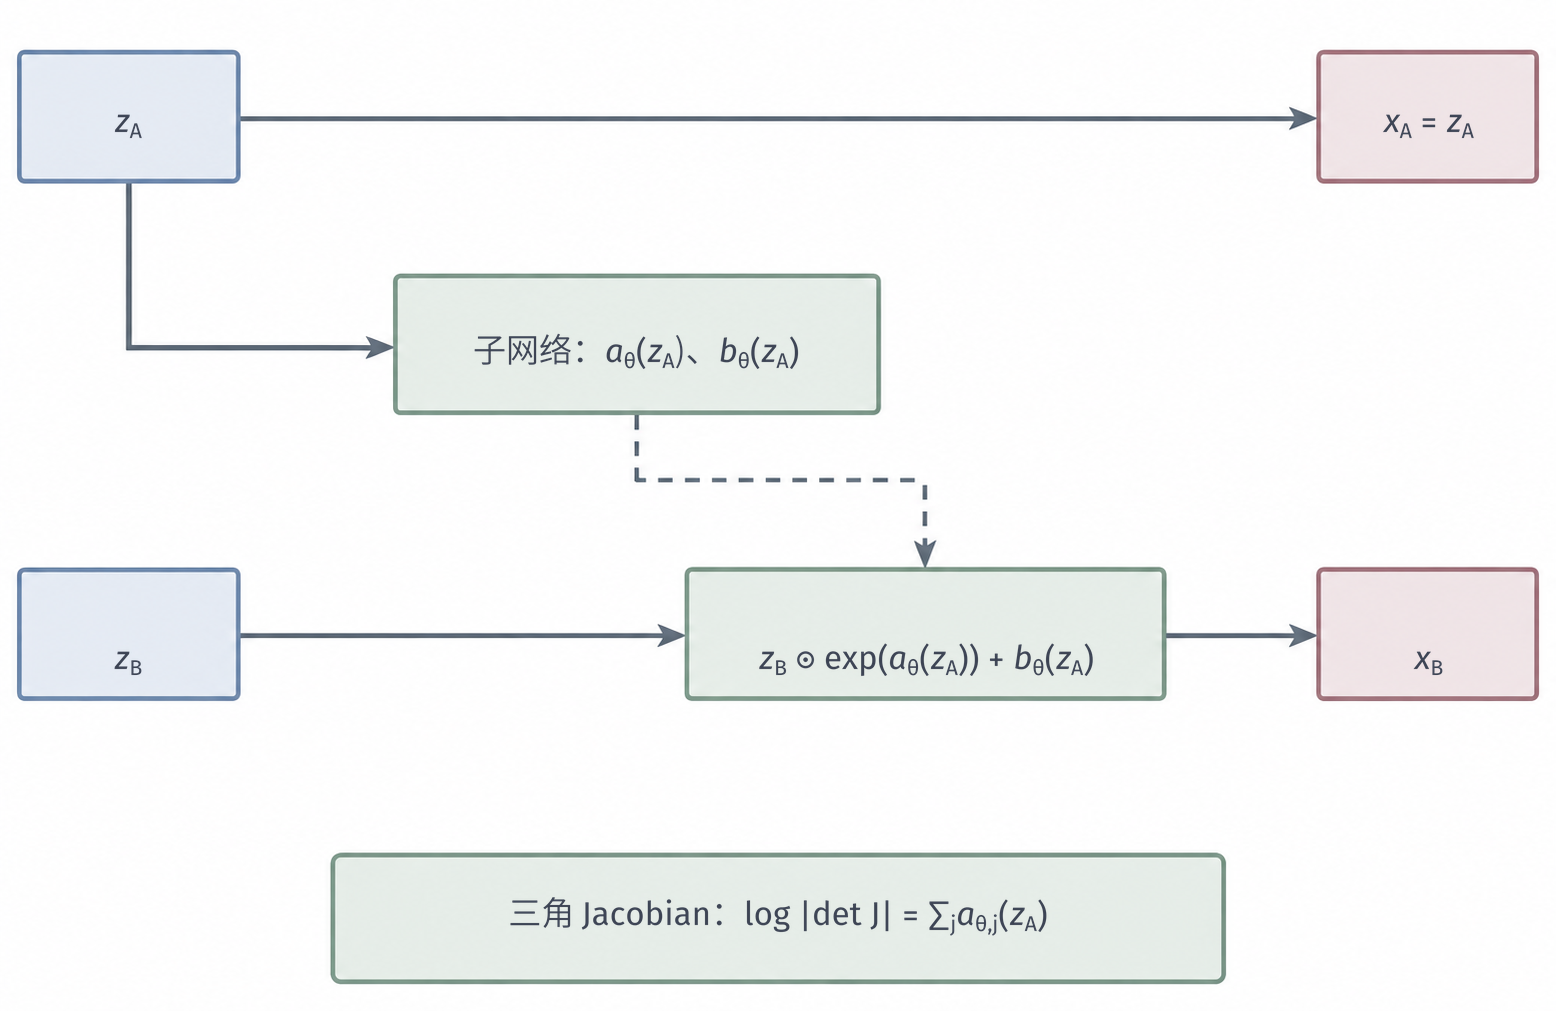
\includegraphics[width=112.000mm]{figures/06-probabilistic-graphical-models/04-models/generated/pgm-generative-coupling/figure.png}
  \caption{仿射耦合层的计算依赖。保留块$\bm z_A$经粗线进入子网络，确定$B$块仿射变换的缩放与平移。Jacobian的下三角结构使对数行列式等于缩放对数之和；逆向计算先恢复$\bm z_A$，再撤销$B$块的平移和缩放。}
  \label{fig:pgm-generative-coupling}
\end{figure}

例如，二维变换$x_1=z_1$、$x_2=2z_2+z_1^2$在$\bm{z}=(1,-1)$处输出$\bm{x}=(1,-1)$，逆变换恢复$z_2=(x_2-x_1^2)/2=-1$。Jacobian为$\left(\begin{smallmatrix}1&0\\2z_1&2\end{smallmatrix}\right)$，行列式恒为$2$。基础分布取二维标准高斯时，该观测的对数密度为$-\log(2\pi)-1-\log2$。非线性项位于Jacobian的非对角块，因此可以改变坐标依赖，同时保留简单的体积因子。

单层保留$A$块，会限制可表达的变换；多层间交换分块或加入可逆混合后，各坐标可以逐步相互影响。

训练仍使用式~\eqref{eq:pgm-generative-flow-objective}，改变的是每层求逆与求体积的算法。二维例中的子网络可以非线性，整体层却因保留块和非零缩放而可逆；增加层数时交替分块，使原先被保留的坐标也能改变。这种结构约束同时决定密度计算成本与能表达的依赖。

\subsection{自回归流的计算方向}
\label{sec:pgm-generative-autoregressive-flow}

另一类让Jacobian好算的办法是借助\emph{坐标顺序}：让第$j$个坐标的变换只依赖它前面的坐标，这样Jacobian天然是下三角、行列式等于对角元之积。这种结构在密度评价和采样两个方向上的代价并不对称，MAF和IAF正是把三角结构放在不同方向而形成互补。\term{自回归流}（autoregressive flow）通过坐标顺序构造三角Jacobian，用前面坐标计算当前可逆变换的参数。与直接参数化条件分布的自回归模型相比，自回归流需要同时考察采样方向和密度评价方向的代价（见第~\ref{chap:pgm-static-directed}章）。\term{掩码自回归流}（masked autoregressive flow, MAF）的一种形式为
\[
  x_j=\mu_j(\bm{x}_{<j})+
       \exp(a_j(\bm{x}_{<j}))z_j,\qquad j=1,\ldots,d,
\]
其中$\bm{x}_{<j}=(x_1,\ldots,x_{j-1})$。评价给定$\bm{x}$时，所有条件输入已知，掩码网络可并行给出各$\mu_j,a_j$，从而恢复$\bm{z}$并求出三角Jacobian的行列式；生成时$\bm{x}_{<j}$尚未齐备，必须顺序恢复坐标。

\term{逆自回归流}（inverse autoregressive flow, IAF）将参数输入改为$\mu_j(\bm{z}_{<j})$和$a_j(\bm{z}_{<j})$。全部基础噪声已知时，输出及对应样本密度可并行计算；给定外部观测后，逆变换则需要逐坐标恢复基础变量。因此，IAF适合生成并评价自身样本，MAF适合评价指定观测的密度，二者的顺序代价分别位于不同方向\scite{pgm-generative-papamakarios2017}

MAF和IAF作为观测空间密度模型时，都把自身逆变换与三角体积项代入式~\eqref{eq:pgm-generative-flow-objective}，差别在给定外部观测后哪些量可以同时计算。若把IAF放进VAE近似后验，则外层目标改为ELBO，生成的是当前观测的潜样本；这一部件角色将在第~\ref{sec:pgm-generative-flow-roles}节展开。直接自回归模型用条件乘积定义观测密度，自回归流则用三角双射定义它，二者共享顺序信息，但不因此成为同一种概率构造。

\subsection{连续规范化流的结构与学习}
\label{sec:pgm-generative-cnf}

离散的流是有限多个可逆层叠起来；若让每一层的改动趋于无穷小、层数趋于无穷，就可以把整个变换描述成一个随连续“时间”演化的\emph{速度场}（常微分方程）。好处是不必再为每层设计三角行列式，只需沿轨迹\emph{累积局部体积的变化率}（速度场的散度）即可。离散Flow把有限个映射复合；当每步接近恒等、并且近似随步长收敛时，可以把移动拆成连续的小步，以速度场描述样本如何迁移。这样不再逐层设计三角行列式，而是累计局部体积的变化率。

连续变换用速度场代替有限层映射。\term{连续规范化流}（continuous normalizing flow, CNF）以常微分方程
\[
  \frac{\mathrm{d}\bm{h}_u}{\mathrm{d}u}
    =\bm{v}_{\bm{\theta}}(\bm{h}_u,u),
  \qquad 0\leq u\leq1,
\]
定义基础变量到观测的映射，起点为$\bm{h}_0=\bm{z}$，终点为$\bm{h}_1=\bm{x}$，$u$表示变换进度。可逆流的一种充分正则设定是：速度场对空间连续可微，满足保证初值问题解唯一性的Lipschitz条件，且解在整个区间正反两向都存在。解的唯一性使不同轨迹在同一进度处保持分离，从而建立一一对应的变换。

记$\rho_u$为$\bm{h}_u$的密度。小步映射的Jacobian为$\bm{I}+\Delta u\,\bm{J}_{\bm{v}}+o(\Delta u)$，结合$\log\det(\bm{I}+\Delta u\,\bm{A})=\Delta u\,\operatorname{tr}\bm{A}+o(\Delta u)$，可从式~\eqref{eq:pgm-generative-flow-density}得到\term{瞬时变量变换公式}（instantaneous change of variables）：
\begin{equation}
  \label{eq:pgm-generative-instantaneous-change}
  \begin{aligned}
    \frac{\mathrm{d}}{\mathrm{d}u}
         \log\rho_u(\bm{h}_u)
       &=-\nabla_{\bm{h}}\!\cdot
          \bm{v}_{\bm{\theta}}(\bm{h}_u,u),\\
    \log p_{\bm{\theta}}(\bm{x})
       &=\log p_0(\bm{z})
         -\int_0^1\nabla_{\bm{h}}\!\cdot
           \bm{v}_{\bm{\theta}}(\bm{h}_u,u)\,\mathrm{d}u.
  \end{aligned}
\end{equation}
散度$\nabla\cdot\bm{v}=\sum_j\partial v_j/\partial h_j$为Jacobian的迹，表示局部体积膨胀率。积分该膨胀率即可追踪密度，因此CNF允许一般的速度场结构，代价转为沿轨迹反复评价速度场与散度。

高维迹计算可以采用随机估计。若随机向量满足$\mathbb{E}\bm{r}=\bm{0}$和$\mathbb{E}\bm{r}\bm{r}^{\top}=\bm{I}$，便有$\operatorname{tr}\bm{A}=\mathbb{E}_{\bm{r}}[\bm{r}^{\top}\bm{A}\bm{r}]$。自动微分通过向量与Jacobian的乘积计算单次估计，FFJORD将这一方法用于连续流\scite{pgm-generative-grathwohl2018}

该恒等式保证固定矩阵下的迹估计无偏，有限样本仍有蒙特卡洛波动。程序还需近似求解状态轨迹和散度积分，因此连续流返回的似然通常同时包含随机估计误差与数值积分误差。正向和逆向计算都依赖求解器，其成本由函数评价次数和速度场的数值性质决定。

在这里约定的生成方向上，CNF的本地目标为
\begin{equation}
  \label{eq:pgm-generative-cnf-objective}
  \min_{\bm\theta}\;\frac1n\sum_i
   \left[-\log p_0(\bm h_{i,0})+
     \int_0^1\nabla_{\bm h}\!\cdot
          \bm v_{\bm\theta}(\bm h_{i,u},u)\,\mathrm du\right],
  \qquad \bm h_{i,1}=\bm x_i.
\end{equation}
每条观测从$u=1$逆向求解到$u=0$，得到基础点及同一路径上的散度积分，再对速度场参数计算梯度。梯度可以通过离散求解计算图传播，或在适用条件下使用连续伴随方法；二者都要面对数值求解与反向误差，不能仅凭连续公式保证程序返回精确梯度。生成则从基础样本向$u=1$积分。连续流的瞬时换元与似然学习可参考Chen等的构造\scite{pgm-generative-chen2018}

有限层可逆映射与ODE流仍有结构差别。若一个离散变换恰好等于同一空间上某个ODE的有限时间解映射，才称它能够嵌入这样的连续流。在前述正则条件下，解映射从恒等映射开始，其Jacobian行列式等于沿途散度积分的指数，因而保持正号。反射$x=-z$是一维合法的离散Flow，导数却恒为$-1$，所以不能由这一维上的上述ODE在有限时间实现。因而近恒等小步的连续化需要条件，任意离散Flow不自动可嵌入同维CNF。接下来要建立的扩散联系，是把特定分数速度场放入CNF。

\section{基于逐步去噪的分布构造}

\label{sec:pgm-generative-diffusion}

\label{sec:pgm-generative-diffusion-structure}

扩散模型走了一条最“绕”、却在实践中极有效的路：不直接学“从噪声一步跳到清晰数据”这一个大跳跃，而是\emph{先反过来}定义一个固定的、不含可学参数的“破坏”过程——把一张真实图片一步步加噪，经过很多步后变成纯高斯噪声；由于每一步怎么加噪是我们自己定的，任意噪声程度的训练样本都能\emph{直接造出来}，于是“从噪声中去掉一点噪”就变成了有标准答案的监督学习任务，相当于自动获得了无限多带标签的去噪训练对。学完每一步的去噪规律后，生成时再从纯噪声出发、一步步反向去噪即可。这样把一个难的生成问题拆解成大量简单的局部去噪问题。对复杂观测，直接拟合从简单噪声到数据的一次映射可能把许多不同变化挤在同一函数中。逐步去噪的想法是先规定怎样逐渐破坏已有样本，再学习每个噪声尺度上怎样生成较清晰的状态。训练数据因而提供大量可构造的局部监督。加噪后同一个状态可能来自多个原样本，逆向学习要描述这些可能性形成的条件分布，不能要求每次找回原来的那一个样本。

\subsection{前向扰动与逆向生成结构}

\label{sec:pgm-generative-forward-reverse}

\term{扩散模型}（diffusion model）用逐步扰动把数据分布与简单噪声分布连接起来，并学习从噪声到数据的局部转移。训练观测提供前向加噪状态，生成则沿相反顺序执行学得的转移。下文的$\bm{x}_t$表示某一噪声尺度下的状态，索引$t$由模型人为构造；真实序列的时间索引另由动态有向模型描述（见第~\ref{chap:pgm-dynamic}章）。

\term{去噪扩散概率模型}（denoising diffusion probabilistic model, DDPM）的一种标准前向过程固定噪声日程$0<\beta_t<1$，$t=1,\ldots,T$，并定义
\begin{equation}
  \label{eq:pgm-generative-forward-chain}
  \begin{aligned}
    q(\bm{x}_{1:T}\mid\bm{x}_0)
      &=\prod_{t=1}^{T}q(\bm{x}_t\mid\bm{x}_{t-1}),\\
    q(\bm{x}_t\mid\bm{x}_{t-1})
      &=\mathcal{N}(\bm{x}_t;
          \sqrt{\alpha_t}\bm{x}_{t-1},\beta_t\bm{I}_d),\\
    \alpha_t&=1-\beta_t,\qquad
    \bar{\alpha}_t=\prod_{s=1}^{t}\alpha_s,\qquad
    \bar{\alpha}_0=1.
  \end{aligned}
\end{equation}
每一步缩小信号并加入独立高斯噪声。条件均值逐步乘以信号衰减系数，条件噪声方差则满足递推$\alpha_t(1-\bar{\alpha}_{t-1})+\beta_t=1-\bar{\alpha}_t$。因此，给定原观测的任意一步分布为
\begin{equation}
  \label{eq:pgm-generative-forward-marginal}
  \begin{aligned}
    q(\bm{x}_t\mid\bm{x}_0)
      &=\mathcal{N}(\bm{x}_t;
          \sqrt{\bar{\alpha}_t}\bm{x}_0,
          (1-\bar{\alpha}_t)\bm{I}_d),\\
    \bm{x}_t&=\sqrt{\bar{\alpha}_t}\bm{x}_0+
              \sqrt{1-\bar{\alpha}_t}\bm{\epsilon},
    \quad \bm{\epsilon}\sim\mathcal{N}(\bm{0},\bm{I}_d).
  \end{aligned}
\end{equation}
训练时可从该条件分布直接抽取任意噪声步，省去之前的逐步扰动计算。式中的标准高斯变量代表当前一步的合成噪声；完整前向路径的跨步依赖仍由式~\eqref{eq:pgm-generative-forward-chain}的逐步独立扰动决定。上述构造及后续目标采用DDPM的固定日程设定\scite{pgm-generative-ho2020}

有限步下，正的$\bar{\alpha}_T$使终点通常仍保留一部分数据结构。生成模型以标准高斯$p(\bm{x}_T)=\mathcal{N}(\bm{0},\bm{I}_d)$作为终端先验，日程需要使前向终点充分接近它。给定原观测时，两者的差距可以通过高斯KL直接计算：
\begin{equation}
  \label{eq:pgm-generative-terminal-kl}
  \begin{aligned}
    &\operatorname{KL}\bigl(
        q(\bm{x}_T\mid\bm{x}_0)\,\|\,p(\bm{x}_T)\bigr)\\
    &\quad=\frac12\left[
       \bar{\alpha}_T\lVert\bm{x}_0\rVert_2^2
       -d\bar{\alpha}_T-d\log(1-\bar{\alpha}_T)
      \right].
  \end{aligned}
\end{equation}
数据二阶矩有限且$\bar{\alpha}_T\to0$时，该条件KL的数据平均趋于零。KL的凸性又使这一平均量控制前向终点边缘$q_T$与先验的KL。有限步下，匹配程度取决于累计信号衰减、数据尺度和观测维度，可用该表达式评价日程选择。

在贯穿例子$X_0\sim\mathcal{N}(0,5)$中，前向边缘可以直接算出：
\begin{equation}
  \label{eq:pgm-generative-gaussian-diffusion}
  q_t(x)=\mathcal{N}(x;0,1+4\bar{\alpha}_t).
\end{equation}
取$\bar{\alpha}_T=0.25$时，终点边缘为$\mathcal{N}(0,2)$，与标准高斯的KL为$\tfrac12(2-1-\log2)\approx0.15343$。取$\bar{\alpha}_T=0.01$时，方差降至$1.04$，KL约为$0.000390$。这里评价的是终点边缘的差距；式~\eqref{eq:pgm-generative-terminal-kl}评价给定原观测的条件差距，其数据平均通常更大。

逆向生成从终端先验抽样，再逐步生成较低噪声状态：
\begin{equation}
  \label{eq:pgm-generative-reverse-joint}
  \begin{aligned}
    p_{\bm{\theta}}(\bm{x}_{0:T})
      &=p(\bm{x}_T)
          \prod_{t=1}^{T}p_{\bm{\theta}}
             (\bm{x}_{t-1}\mid\bm{x}_t),\\
    p_{\bm{\theta}}(\bm{x}_0)
      &=\int p_{\bm{\theta}}(\bm{x}_{0:T})
               \,\mathrm{d}\bm{x}_{1:T}.
  \end{aligned}
\end{equation}
终端先验和每个逆转移归一化时，联合分布及观测边缘随之归一化。中间状态作为与观测同维的潜变量，使离散扩散具有有向潜变量模型的形式。其近似推断路径由固定前向扰动核给出，因此训练可以直接构造路径样本。

\begin{figure}[htbp]
  \centering
  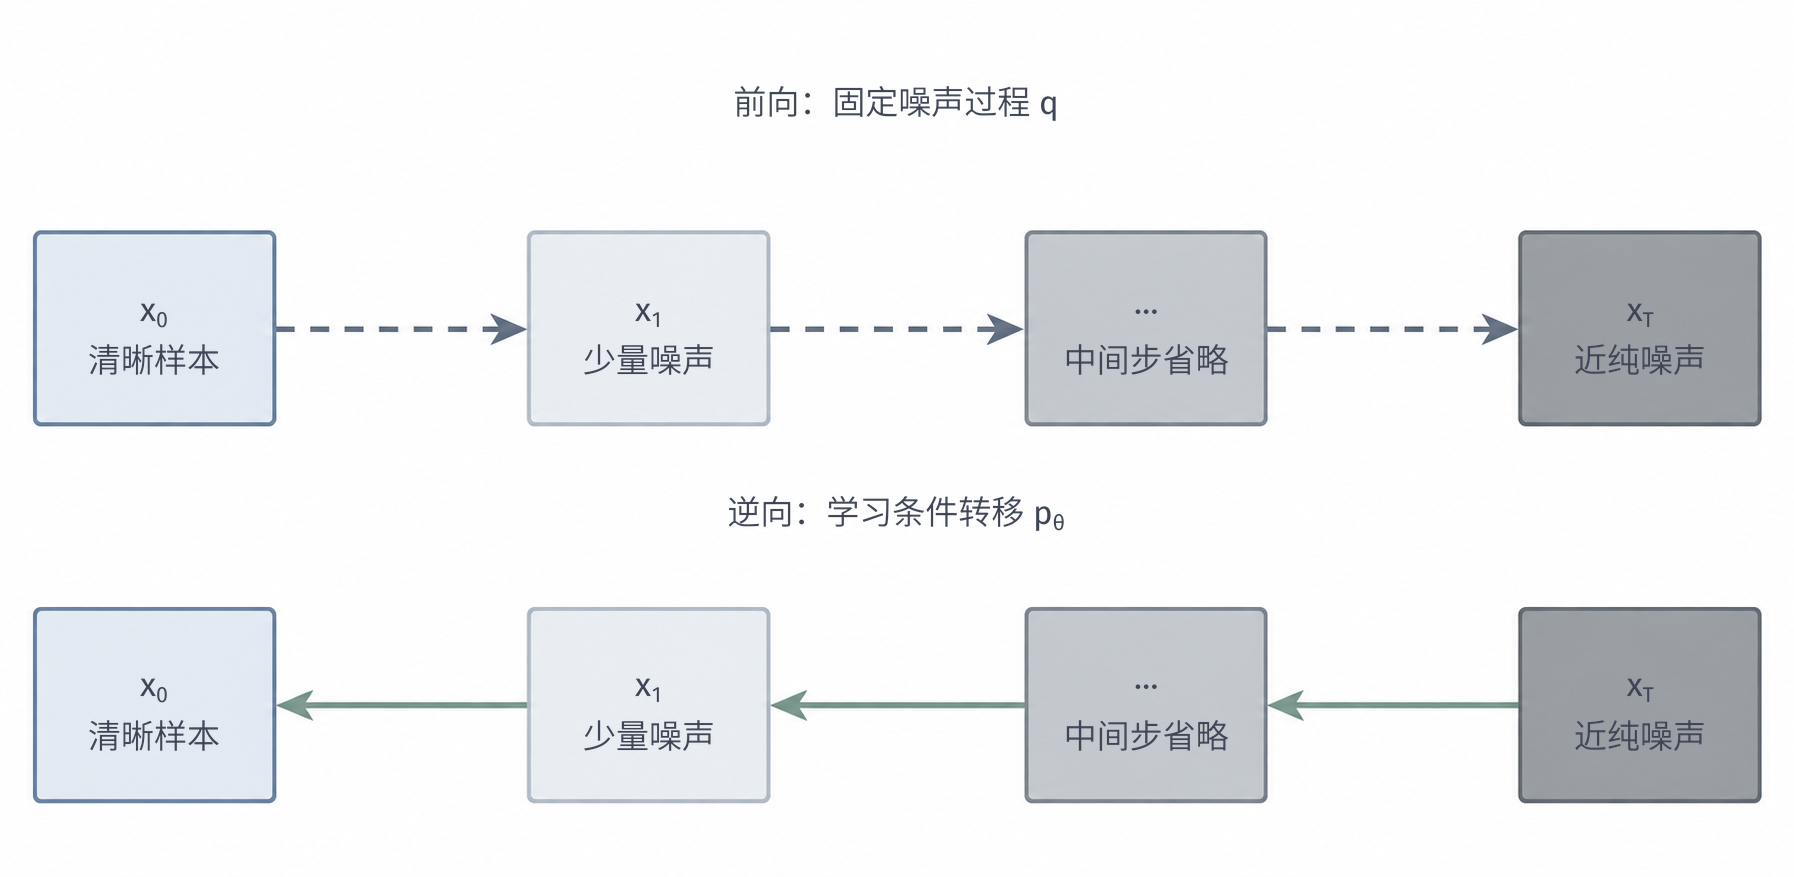
\includegraphics[width=112.000mm]{figures/06-probabilistic-graphical-models/04-models/generated/pgm-generative-diffusion/figure.png}
  \caption{离散扩散的前向扰动与逆向生成。上行按固定日程逐步加噪，下行从终端先验开始执行学得的逆转移。灰度与文字表示状态的噪声程度，相同下标对应相同噪声尺度。两行分别抽样；有限步下的终点匹配由日程和数据尺度决定。}
  \label{fig:pgm-generative-diffusion}
\end{figure}

图~\ref{fig:pgm-generative-diffusion}中的模型逆转移通常采用神经网络参数化的高斯均值与方差。真实逆转移$q(\bm{x}_{t-1}\mid\bm{x}_t)$还需对未知原观测混合，一般具有更复杂的分布形状。后续学习目标中的解析高斯则额外给定原观测，描述$q(\bm{x}_{t-1}\mid\bm{x}_t,\bm{x}_0)$。因此，小步高斯是有限步模型的参数化选择，其逼近误差需要与原观测已知时的解析计算区分。

图~\ref{fig:diffusion-sample-process-illustration}通过样本插画表示噪声尺度的变化。下行以独立终端噪声启动学得的生成链，上行则由给定样本启动固定扰动链。

\begin{figure*}[htbp]
  \centering
  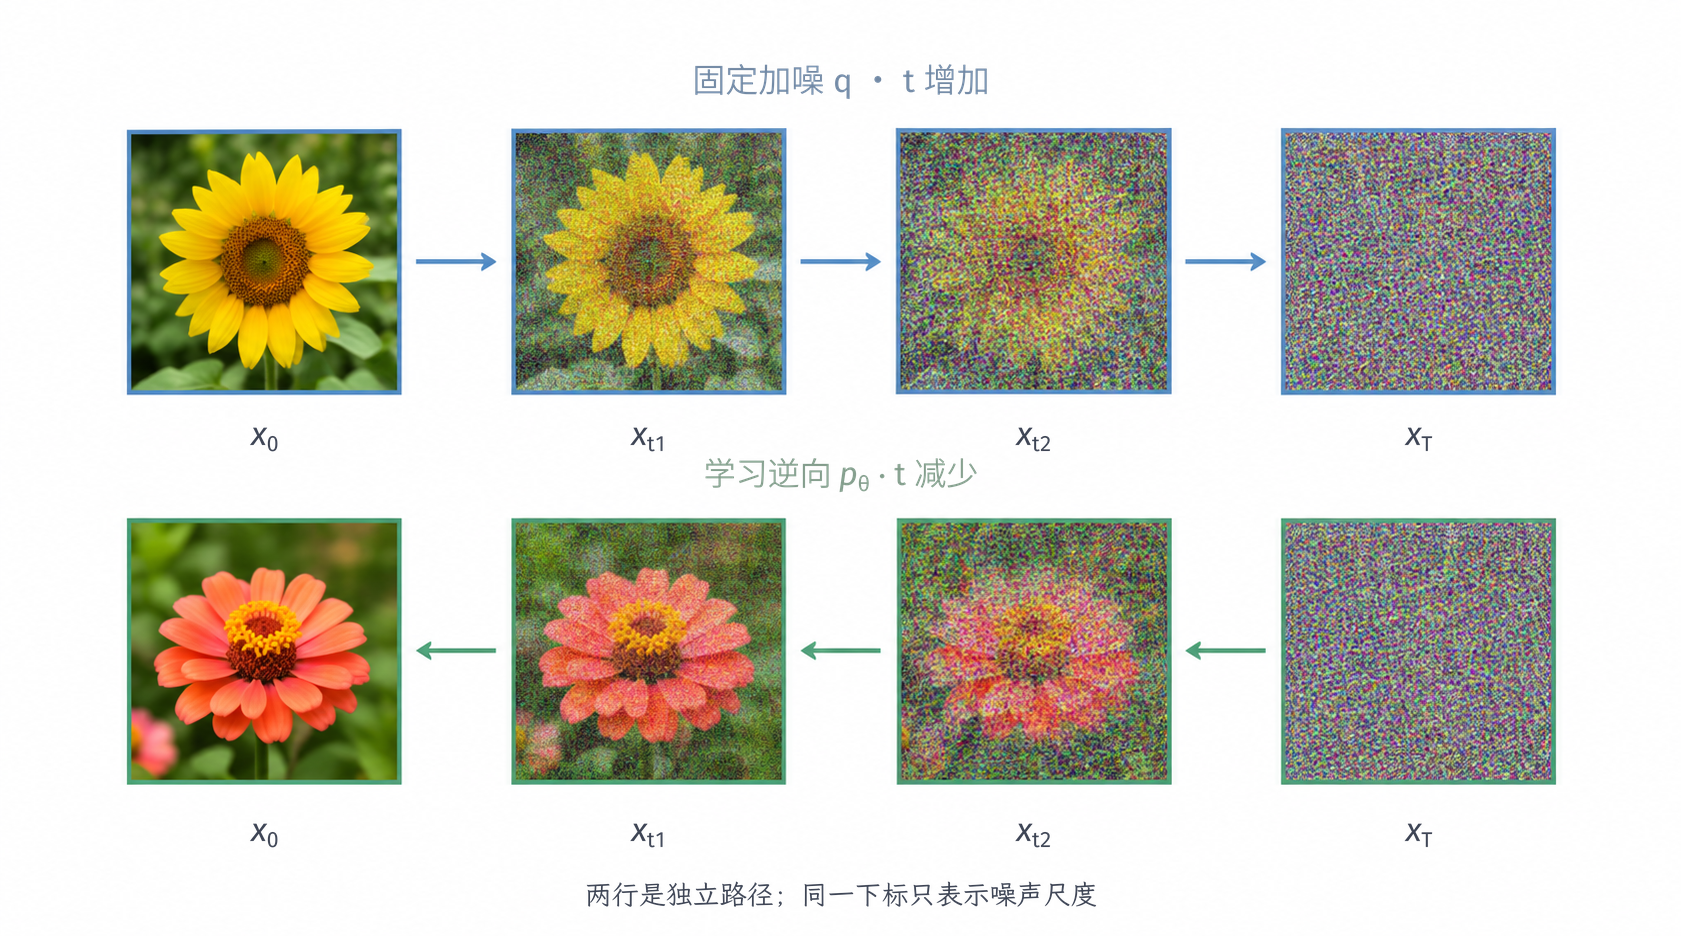
\includegraphics[width=139.534mm]{figures/06-probabilistic-graphical-models/04-models/generated/diffusion-sample-process-illustration/figure.png}
  \caption{扩散链的样本变化示意。上行从左向右逐步扰动观测，下行从右侧独立终端噪声开始向左生成；下标记录噪声尺度。花朵及中间状态为机制插画，用于说明扰动与生成方向。}
  \label{fig:diffusion-sample-process-illustration}
\end{figure*}

至此，固定日程决定前向分布，逆转移网络决定生成族。网络每次读取$(\bm x_t,t)$，输出逆转移均值，或输出能够换算成该均值的噪声预测；方差可以按日程固定，也可以另设受约束的正方差输出。生成参数出现在逆向链中，训练用的前向核则是我们预先选择的计算工具。下面把两者放入一个明确的学习目标。

\subsection{潜路径积分与变分学习目标}

\label{sec:pgm-generative-diffusion-learning}

\label{sec:pgm-generative-diffusion-objective}

逆向生成联合分布的学习可以采用路径变分下界。将观测固定为$\bm{x}_0$，以整条中间路径$\bm{x}_{1:T}$为潜变量，并用前向扰动分布作近似后验，一般ELBO便成为联合与前向路径密度比的期望（见式~\eqref{eq:pgm-variational-elbo}）。记路径下界为$\mathcal{B}_{\mathrm{diff}}(\bm{x}_0)$，其负值为$\mathcal{J}_{\mathrm{diff}}=-\mathcal{B}_{\mathrm{diff}}$：
\begin{equation}
  \label{eq:pgm-generative-path-elbo}
  \begin{aligned}
    \log p_{\bm{\theta}}(\bm{x}_0)
      &\geq\mathcal{B}_{\mathrm{diff}}(\bm{x}_0),\\
    \mathcal{J}_{\mathrm{diff}}(\bm{x}_0)
      &=\mathbb{E}_{q(\bm{x}_{1:T}\mid\bm{x}_0)}
         \left[\log
           \frac{q(\bm{x}_{1:T}\mid\bm{x}_0)}
                {p_{\bm{\theta}}(\bm{x}_{0:T})}
         \right].
  \end{aligned}
\end{equation}

要把这个路径比值化为局部计算，使用$t\geq2$时的Bayes恒等式
\[
  q(\bm{x}_t\mid\bm{x}_{t-1})
  =q(\bm{x}_{t-1}\mid\bm{x}_t,\bm{x}_0)
     \frac{q(\bm{x}_t\mid\bm{x}_0)}
          {q(\bm{x}_{t-1}\mid\bm{x}_0)}.
\]
将该恒等式代入前向路径密度，相邻边缘比值消去，得到同一路径密度的反向分解：
\[
  \begin{aligned}
    q(\bm{x}_{1:T}\mid\bm{x}_0)
      ={}&q(\bm{x}_T\mid\bm{x}_0)\\
         &{}\times\prod_{t=2}^{T}
              q(\bm{x}_{t-1}\mid\bm{x}_t,\bm{x}_0).
  \end{aligned}
\]
再对每个中间变量取条件期望，路径目标便分解为可局部评价的项：
\begin{equation}
  \label{eq:pgm-generative-ddpm-kl}
  \begin{aligned}
    \mathcal{J}_{\mathrm{diff}}(\bm{x}_0)
      ={}&\operatorname{KL}\bigl(
          q(\bm{x}_T\mid\bm{x}_0)\,\|\,p(\bm{x}_T)\bigr)\\
       &+\sum_{t=2}^{T}
         \mathbb{E}_{q(\bm{x}_t\mid\bm{x}_0)}
          \operatorname{KL}\bigl(
           q(\bm{x}_{t-1}\mid\bm{x}_t,\bm{x}_0)
           \,\|\,p_{\bm{\theta}}(\bm{x}_{t-1}\mid\bm{x}_t)
                         \bigr)\\
       &-\mathbb{E}_{q(\bm{x}_1\mid\bm{x}_0)}
          \log p_{\bm{\theta}}(\bm{x}_0\mid\bm{x}_1).
  \end{aligned}
\end{equation}

三部分分别评价终点匹配、逐步逆转移匹配和观测解码。固定日程与先验后，终点项与学习参数无关，求梯度时可以省略，报告完整似然界时仍计入其值。解码项评价已知观测的条件对数似然；它与中间变量的高斯KL具有不同形式，因为原观测在此已经固定。

给定原观测后，前向过程中的高斯结构使中间KL具有解析形式。对$t\geq2$，将$q(\bm{x}_t\mid\bm{x}_{t-1})q(\bm{x}_{t-1}\mid\bm{x}_0)$按待求中间变量配平方，二次项的精度系数为
\[
  \frac{\alpha_t}{\beta_t}
    +\frac{1}{1-\bar{\alpha}_{t-1}}
  =\frac{1-\bar{\alpha}_t}
          {\beta_t(1-\bar{\alpha}_{t-1})}.
\]
线性项为$\sqrt{\alpha_t}\bm{x}_t/\beta_t+\sqrt{\bar{\alpha}_{t-1}}\bm{x}_0/(1-\bar{\alpha}_{t-1})$。精度的倒数给出方差，方差与线性项相乘给出均值，因此条件分布为
\begin{equation}
  \label{eq:pgm-generative-forward-posterior}
  \begin{aligned}
    q(\bm{x}_{t-1}\mid\bm{x}_t,\bm{x}_0)
      &=\mathcal{N}(\bm{x}_{t-1};
          \widetilde{\bm{\mu}}_t,\widetilde{\beta}_t\bm{I}_d),\\
    \widetilde{\beta}_t
      &=\frac{\beta_t(1-\bar{\alpha}_{t-1})}
              {1-\bar{\alpha}_t},\\
    \widetilde{\bm{\mu}}_t
      &=\frac{\sqrt{\bar{\alpha}_{t-1}}\beta_t}
               {1-\bar{\alpha}_t}\bm{x}_0
       +\frac{\sqrt{\alpha_t}(1-\bar{\alpha}_{t-1})}
               {1-\bar{\alpha}_t}\bm{x}_t.
  \end{aligned}
\end{equation}
训练观测已知，可以直接计算这一条件均值作为监督目标。生成时只能使用当前状态、噪声步和给定外部条件，因此模型需要学习从这些输入预测相应均值。

现固定逆转移方差$\sigma_t^2>0$，令$p_{\bm{\theta}}(\bm{x}_{t-1}\mid\bm{x}_t)=\mathcal{N}(\bm{\mu}_{\bm{\theta}}(\bm{x}_t,t),\sigma_t^2\bm{I}_d)$。高斯KL分为均值误差与方差误差：
\begin{equation}
  \label{eq:pgm-generative-gaussian-step-kl}
  \begin{aligned}
    \operatorname{KL}(q\,\|\,p_{\bm{\theta}})
      &=\frac{\lVert\widetilde{\bm{\mu}}_t
                    -\bm{\mu}_{\bm{\theta}}(\bm{x}_t,t)\rVert_2^2}
               {2\sigma_t^2}+C_t,\\
    C_t&=\frac{d}{2}
       \left(\frac{\widetilde{\beta}_t}{\sigma_t^2}
              -1+\log\frac{\sigma_t^2}{\widetilde{\beta}_t}\right).
  \end{aligned}
\end{equation}
固定逆转移方差时，方差项$C_t$与待学习参数无关，常用选择为$\sigma_t^2=\beta_t$或在$t\geq2$时取$\sigma_t^2=\widetilde{\beta}_t$。逆转移方差参与学习时，均值误差权重与方差项都随参数变化，需要共同优化。若逆转移方差依赖当前状态而无待学习参数，方差项仍可在求梯度时省略，其数值则同时依赖状态与噪声步。

\subsection{噪声目标与具体训练步骤}
\label{sec:pgm-generative-noise-training}

利用式~\eqref{eq:pgm-generative-forward-marginal}把$\bm{x}_0$换成$\bm{x}_t$和噪声，后验均值也可写成
\[
  \widetilde{\bm{\mu}}_t
  =\frac{1}{\sqrt{\alpha_t}}
       \left(\bm{x}_t-
          \frac{\beta_t}{\sqrt{1-\bar{\alpha}_t}}\bm{\epsilon}\right).
\]
该形式将均值学习转换为合成噪声预测。用网络$\bm{\epsilon}_{\bm{\theta}}(\bm{x}_t,t)$预测噪声，并据此定义模型均值：
\begin{equation}
  \label{eq:pgm-generative-noise-parameterization}
  \bm{\mu}_{\bm{\theta}}(\bm{x}_t,t)
  =\frac{1}{\sqrt{\alpha_t}}
       \left(\bm{x}_t-
          \frac{\beta_t}{\sqrt{1-\bar{\alpha}_t}}
               \bm{\epsilon}_{\bm{\theta}}(\bm{x}_t,t)\right).
\end{equation}
回到仅随噪声步变化的固定逆转移方差设定，两均值相减时$\bm{x}_t$项抵消。记$\ell_t(\bm{\theta})$为第$t$个中间KL的数据与扰动平均，并仍按式~\eqref{eq:pgm-generative-forward-marginal}抽取$\bm{x}_t$，则
\begin{equation}
  \label{eq:pgm-generative-weighted-denoising}
  \begin{aligned}
    \ell_t(\bm{\theta})
      &=w_t\,\mathbb{E}_{\bm{x}_0,\bm{\epsilon}}
         \lVert\bm{\epsilon}
          -\bm{\epsilon}_{\bm{\theta}}(\bm{x}_t,t)\rVert_2^2+C_t,\\
    w_t&=\frac{\beta_t^2}
              {2\sigma_t^2\alpha_t(1-\bar{\alpha}_t)},
          \qquad t=2,\ldots,T.
  \end{aligned}
\end{equation}
这一权重由固定逆转移方差下的高斯KL推导而来，通常随噪声步变化，因此决定不同噪声尺度对ELBO学习的相对贡献。

\begin{example}[核对一个扩散步的权重]
  \label{ex:pgm-generative-step-weight}
  取便于手算的噪声系数$\beta_1=0.2$、$\beta_2=0.25$，于是$\alpha_2=0.75$、$\bar{\alpha}_1=0.8$、$\bar{\alpha}_2=0.6$。在$t=2$时，给定原观测的条件方差为$\widetilde{\beta}_2=0.25(0.2)/0.4=0.125$。若模型逆转移方差取$\sigma_2^2=0.25$，去噪权重为$w_2=0.25^2/(2\cdot0.25\cdot0.75\cdot0.4)=5/12$。一维噪声预测误差取$0.3$，对应均值差的平方为
  \[
    \frac{0.25^2}{0.75\cdot0.4}(0.3)^2=0.01875,
  \]
  除以$2\sigma_2^2=0.5$得到$0.0375$，与$(5/12)(0.3)^2$一致。再加方差项$C_2=\tfrac12(0.5-1+\log2)\approx0.09657$，便得到完整KL。本例用较大的噪声系数核对均值参数化与去噪权重的代数关系。
\end{example}

DDPM还常用均匀抽步的噪声平方回归作为简化目标。独立抽取$t\sim\operatorname{Unif}\{1,\ldots,T\}$、$\bm{x}_0\sim p_{\mathrm{data}}$和$\bm{\epsilon}\sim\mathcal{N}(\bm{0},\bm{I}_d)$，定义
\begin{equation}
  \label{eq:pgm-generative-simple-loss}
  \mathcal{J}_{\mathrm{simple}}
  =\mathbb{E}_{t,\bm{x}_0,\bm{\epsilon}}
      \lVert\bm{\epsilon}
       -\bm{\epsilon}_{\bm{\theta}}(\bm{x}_t,t)\rVert_2^2.
\end{equation}
该目标为所有噪声步采用相同回归权重，并在$t=1$继续预测噪声。它改变了原ELBO中各尺度的权衡，报告似然下界时需回到完整路径目标。原始DDPM对离散像素以量化区间积分定义解码质量；连续数据采用固定方差高斯解码时，解码负对数似然则包含特定权重的平方误差及常数项。因此，简化噪声损失与这些解码项、逐步加权KL的数值不同\scite{pgm-generative-ho2020}

严格ELBO也可以通过随机抽步优化。对中间步按正概率$\pi_t$抽取$t\in\{2,\ldots,T\}$，用$w_t\lVert\bm{\epsilon}-\bm{\epsilon}_{\bm{\theta}}\rVert_2^2/\pi_t$无偏估计其中依赖参数的求和，并单独计算解码项。均匀抽步时，校正因子为中间步数；报告完整界值还需计入方差常数和终点项。

抽步概率的改变配合重要性校正，可以调整估计方差而保留原目标。直接改变步权重则调整训练准则。若模型表达能力不受限、各尺度可独立拟合，任意正权重都保留逐尺度平方回归的最优条件均值；有限共享网络需在不同尺度间分配容量，权重因而影响实际拟合结果。

对有限数据，将式~\eqref{eq:pgm-generative-simple-loss}中的数据期望换成训练记录的平均，便得到实际小批量训练的经验目标。每次独立抽取记录、噪声步和标准高斯噪声，利用直接扰动公式生成$\bm x_t$，把$(\bm x_t,t)$送入共享网络，再对约定权重的平方误差更新$\bm\theta$。训练不必先逐步构造整条前向路径；被抽到的噪声尺度决定这一轮采用的受扰动输入和监督信号，也影响学习难度。验证目标与生成评价分别记录，并在预先约定的预算或停止条件下结束。

\subsection{学得模型的祖先采样}
\label{sec:pgm-generative-ancestral-generation}

无条件生成不以某条原始观测作为输入或条件。生成从已指定的终端先验出发，依据当前状态计算下一转移，再从该条件分布抽样。由于逆向生成联合本身按这些条件相乘，完整执行下列步骤就是所定义离散模型的祖先采样。

算法~\ref{alg:pgm-generative-ddpm}采用连续观测，逆转移方差均预先固定且为正。全部转移均值由噪声网络按式~\eqref{eq:pgm-generative-noise-parameterization}计算，包括$t=1$的高斯解码分布$p_{\bm{\theta}}(\bm{x}_0\mid\bm{x}_1)$。同一噪声损失因而训练各步均值，解码阶段使用这组共享参数。

\par\noindent\begin{minipage}{\linewidth}
\begin{algorithm}[固定方差DDPM的学习与祖先采样]
  \label{alg:pgm-generative-ddpm}
  \begin{algorithmic}[1]
    \Require 连续观测数据集、固定$\beta_{1:T}$及正的逆转移方差$\sigma_{1:T}^2$
    \Ensure 学得的噪声网络与模型样本
    \State 初始化$\bm{\theta}$，预计算$\alpha_t,\bar{\alpha}_t$
    \For{每个训练小批量，直至停止条件满足}
      \State 为每个观测抽$t\sim\operatorname{Unif}\{1,\ldots,T\}$和标准高斯$\bm{\epsilon}$
      \State 按式~\eqref{eq:pgm-generative-forward-marginal}计算$\bm{x}_t$
      \State 由式~\eqref{eq:pgm-generative-simple-loss}更新参数
    \EndFor
    \State 抽$\bm{x}_T\sim\mathcal{N}(\bm{0},\bm{I}_d)$
    \For{$t=T,T-1,\ldots,2$}
      \State 用噪声网络和式~\eqref{eq:pgm-generative-noise-parameterization}计算$\bm{\mu}_{\bm{\theta}}$
      \State 独立抽$\bm{\xi}_t\sim\mathcal{N}(\bm{0},\bm{I}_d)$，令$\bm{x}_{t-1}=\bm{\mu}_{\bm{\theta}}+\sigma_t\bm{\xi}_t$
    \EndFor
    \State 抽$\bm{x}_0\sim p_{\bm{\theta}}(\bm{x}_0\mid\bm{x}_1)$并返回
  \end{algorithmic}
\end{algorithm}
\end{minipage}\par

算法采用简化训练损失。严格变分学习可将训练步骤替换为带权中间项估计和解码负对数似然。连续高斯解码的末步方差需单独指定正值，因为解析前向后验的$\widetilde{\beta}_1=0$对应已固定的原观测。末步也可以约定输出预测均值，但这种输出省去了正方差解码分布的随机波动。

设一次网络前向代价为$C_{\mathrm{net}}$，随机抽步训练的单样本前向代价约为$O(C_{\mathrm{net}}+d)$，完整祖先采样则为$O(T(C_{\mathrm{net}}+d))$。采样只需保留当前状态；评价全路径变分界还需处理全部项，或采用带校正的随机估计。训练抽步的计算收益因此与多步生成的成本并存。

有限步DDPM的这些转移既决定生成程序，也决定模型边缘密度。跳过其中某步或改成确定性输出，会改变采样规则；只有重新给出相应模型或近似依据，才能判断新输出与原模型的关系。下面先解释已学噪声与密度梯度的联系，再借助连续噪声尺度建立另一种生成描述。

\subsection{从噪声预测到分数估计}
\label{sec:pgm-generative-score-estimation}

预测噪声这件事还有一个更几何的解释：在每个噪声尺度上，它其实等价于在学该尺度分布的\emph{分数函数}，即对数密度对输入的梯度——一个指向“密度往哪个方向上升最快”的向量场。这个视角非常关键，因为它把离散的扩散模型和连续时间理论（反向随机微分方程、概率流）联系了起来。噪声回归还可以理解为密度梯度学习。记前向扰动后的边缘密度为$q_t(\bm{x})$，其\term{分数}（score）$\bm{s}_t^*(\bm{x})=\nabla_{\bm{x}}\log q_t(\bm{x})$给出对数密度局部增加的方向。本章用$q_t$与前向路径记号保持一致，分数模型文献也常将该边缘记为$p_t$。虽然边缘分数未知，高斯扰动的条件分数可以直接计算：
\[
  \nabla_{\bm{x}_t}\log q(\bm{x}_t\mid\bm{x}_0)
  =-\frac{\bm{x}_t-\sqrt{\bar{\alpha}_t}\bm{x}_0}
           {1-\bar{\alpha}_t}
  =-\frac{\bm{\epsilon}}{\sqrt{1-\bar{\alpha}_t}}.
\]
若可以交换微分与积分，对$q_t(\bm{x}_t)=\int q(\bm{x}_t\mid\bm{x}_0)p_{\mathrm{data}}(\bm{x}_0)\,\mathrm{d}\bm{x}_0$求导并除以$q_t(\bm{x}_t)>0$，得到
\begin{equation}
  \label{eq:pgm-generative-denoising-identity}
  \bm{s}_t^*(\bm{x}_t)
  =\mathbb{E}\!\left[
       \nabla_{\bm{x}_t}\log q(\bm{x}_t\mid\bm{X}_0)
       \mid\bm{x}_t\right]
  =-\frac{\mathbb{E}[\bm{\epsilon}\mid\bm{x}_t]}
            {\sqrt{1-\bar{\alpha}_t}}.
\end{equation}
平方回归的总体最优预测为条件均值。因此，令$\bm{s}_{\bm{\theta}}=-\bm{\epsilon}_{\bm{\theta}}/\sqrt{1-\bar{\alpha}_t}$，噪声预测对应各尺度边缘分数的估计。给定受扰动状态后，多种原观测与噪声都可能产生它，回归目标中的随机噪声通过条件平均形成可预测部分。

\term{去噪分数匹配}（denoising score matching, DSM）以已知扰动核的条件分数训练未知边缘分数。令$\bm{a}=\nabla_{\bm{x}_t}\log q(\bm{x}_t\mid\bm{X}_0)$；在平方矩有限时，条件期望的正交分解把训练误差写为
\begin{equation}
  \label{eq:pgm-generative-dsm-decomposition}
  \mathbb{E}\lVert\bm{s}_{\bm{\theta}}-\bm{a}\rVert_2^2
  =\mathbb{E}\lVert\bm{s}_{\bm{\theta}}-\bm{s}_t^*\rVert_2^2
   +\mathbb{E}\lVert\bm{a}-\bm{s}_t^*\rVert_2^2.
\end{equation}
最后一项与网络参数无关，因此最小化条件分数误差等价于最小化边缘分数误差。对当前高斯核，噪声平方误差为条件分数平方误差乘以$(1-\bar{\alpha}_t)$。简化噪声损失与严格ELBO因而对应不同的DSM尺度加权，只有从指定生成模型推导的权重及其余项才组成该模型的ELBO。连续时间分数建模将这些噪声尺度连接起来\scite{pgm-generative-song2021}

把式~\eqref{eq:pgm-generative-noise-parameterization}改用分数表示，还得到
\[
  \bm{\mu}_{\bm{\theta}}(\bm{x}_t,t)
    =\frac{\bm{x}_t+\beta_t\bm{s}_{\bm{\theta}}(\bm{x}_t,t)}
            {\sqrt{\alpha_t}}.
\]
使用真分数时，该式给出真实逆转移的条件均值；转移的完整形状仍由数据分布决定。式~\eqref{eq:pgm-generative-gaussian-diffusion}的一维例子给出真分数$-x_t/(1+4\bar{\alpha}_t)$，代入即可核对均值。

分数也联系能量模型：若$q_t(\bm{x})\propto\exp[-E_t(\bm{x})]$，则$\bm{s}_t^*=-\nabla E_t$，因为归一化常数对空间求导后消失（见第~\ref{chap:pgm-energy-models}章）。一般向量网络近似分数时，还需额外条件才能把它表示为标量能量的梯度；直接评价归一化密度也需要相应密度构造。

\subsection{连续噪声尺度的扰动、学习与逆向生成}

\label{sec:pgm-generative-continuous-diffusion}

细化噪声步后，可以用连续索引$t\in[0,T_{\mathrm{c}}]$描述扰动，$T_{\mathrm{c}}$为终点。本节采用扩散系数仅依赖时间的各向同性设定，使逆向公式具有明确的分数项。设$\bm{W}_t$为$d$维标准\term{布朗运动}（Brownian motion），其不相交区间增量相互独立，长度$\Delta t$的增量服从$\mathcal{N}(\bm{0},\Delta t\,\bm{I}_d)$。前向\term{随机微分方程}（stochastic differential equation, SDE）为
\begin{equation}
  \label{eq:pgm-generative-forward-sde}
  \mathrm{d}\bm{X}_t
  =\bm{b}(\bm{X}_t,t)\,\mathrm{d}t
    +g(t)\,\mathrm{d}\bm{W}_t,
  \qquad \bm{X}_0\sim p_{\mathrm{data}}.
\end{equation}
漂移$\bm{b}$规定确定性的局部移动，$g(t)>0$规定噪声强度。为保证前向解存在且不爆炸，假设系数连续，漂移对空间全局Lipschitz且至多线性增长，噪声系数有界并在所讨论闭区间上有正下界。

使用反向密度公式还需密度和逆过程的正则性：假设$q_t>0$，对时间一阶、对空间二阶连续可微，所用时间区间上$\int\mathbb{E}_{q_t}\lVert\nabla\log q_t(\bm{X}_t)\rVert_2^2\,\mathrm{d}t<\infty$，且反向方程存在不爆炸的解。数据分布本身奇异时，可将这些条件限定于$t\geq\delta>0$的已加噪区间，观测端点另行处理。

与离散DDPM相应的方差保持过程采用$\bm{b}(\bm{x},t)=-\tfrac12\beta(t)\bm{x}$和$g(t)=\sqrt{\beta(t)}$。条件均值的衰减系数为$\exp[-\tfrac12\int_0^t\beta(s)\,\mathrm{d}s]$，条件方差为$1-\exp[-\int_0^t\beta(s)\,\mathrm{d}s]$。有限终点内的累计噪声积分有限时，仍有一部分原信号保留；终点与标准高斯的匹配需要通过累计扰动强度控制。

\paragraph{连续噪声尺度的训练}

条件扰动核可解析时，可以从连续区间抽取噪声尺度，构造受扰动观测，再拟合条件分数$\nabla_{\bm{x}_t}\log q(\bm{x}_t\mid\bm{x}_0)$。式~\eqref{eq:pgm-generative-denoising-identity}和式~\eqref{eq:pgm-generative-dsm-decomposition}在满足条件的每个正噪声尺度上继续说明其边缘分数含义。时间抽样密度与损失权重共同决定训练比重；观测似然评价则需要另外建立密度构造及相应积分计算。

把噪声尺度取在$[\delta,T_{\mathrm c}]$，其中$\delta>0$避开可能奇异的观测端点。为覆盖整个区间，令$r(t)$为指定、归一化且在该区间几乎处处为正的时间抽样密度，$\lambda(t)>0$为尺度权重；二者均不依赖待学习参数。已知可抽样并可评价条件分数的扰动核，且下式的加权平方误差可积时，连续模型的学习目标为
\begin{equation}
  \label{eq:pgm-generative-continuous-dsm-objective}
  \min_{\bm\theta}\;\mathbb E_{
       t\sim r,\,\bm x_0\sim\widehat p_n,\,
       \bm x_t\sim q_t(\cdot\mid\bm x_0)}
    \left[\lambda(t)\left\|
      \bm s_{\bm\theta}(\bm x_t,t)
       -\nabla_{\bm x_t}\log q_t(\bm x_t\mid\bm x_0)
                      \right\|_2^2\right],
\end{equation}
其中$\widehat p_n$表示对训练记录均匀抽样。当前方差保持过程的条件核是均值和方差已知的高斯，所以监督分数可由扰动噪声直接算出。一次更新依次抽记录、连续时间和噪声，计算受扰动状态及目标分数，然后更新共享网络；$r$与$\lambda$共同决定各尺度的训练比重。若$r$在某段子区间为零，目标便只在其支持集上直接监督，不能据此声称覆盖整段尺度。

将抽样梯度用作目标梯度的无偏估计时，仍需交换参数微分与上述联合期望；例如，在参数邻域内可微且导数受可积函数控制。若还要使用有限方差的梯度估计，则需另验梯度二阶矩有限。目标有限、微分交换与梯度方差是分别需要核对的条件。

一般SDE即使能够模拟，也未必有可评价的条件分数；要使用上述去噪目标，还需另行获得这一监督量或采用其他分数学习准则。该目标训练的是密度梯度，其数值本身不是观测对数似然。

记真分数为$\bm{s}_t^*=\nabla_{\bm{x}}\log q_t$。在上述正则条件及反向过程存在的设定下，反向SDE可以沿同一个$t$写成
\begin{equation}
  \label{eq:pgm-generative-reverse-sde}
  \begin{aligned}
    \mathrm{d}\bm{X}_t
    ={}&\bigl[\bm{b}(\bm{X}_t,t)-g(t)^2\bm{s}_t^*(\bm{X}_t)\bigr]
         \,\mathrm{d}t\\
       &+g(t)\,\mathrm{d}\overline{\bm{W}}_t,
    \qquad t:T_{\mathrm{c}}\downarrow0.
  \end{aligned}
\end{equation}
该式沿递减时间积分，$\mathrm{d}t<0$，反向布朗增量的协方差为$|\mathrm{d}t|\bm{I}_d$。实现时可改用递增反向索引$u=T_{\mathrm{c}}-t$，令$\bm{Y}_u=\bm{X}_{T_{\mathrm{c}}-u}$，将时间方向显式写入漂移：
\begin{equation}
  \label{eq:pgm-generative-positive-reverse-time}
  \begin{aligned}
    \mathrm{d}\bm{Y}_u
      ={}&-\bm{b}(\bm{Y}_u,T_{\mathrm{c}}-u)\,\mathrm{d}u\\
         &+g(T_{\mathrm{c}}-u)^2
              \bm{s}_{T_{\mathrm{c}}-u}^*(\bm{Y}_u)\,\mathrm{d}u\\
         &+g(T_{\mathrm{c}}-u)\,\mathrm{d}\bm{B}_u.
  \end{aligned}
\end{equation}
其中$\bm{B}_u$为递增反向索引下的标准布朗运动。该路径反演结果使用真分数及上述正则条件，其证明依赖随机过程反演理论。分数SDE框架还讨论了状态相关扩散系数；相应逆漂移包含扩散矩阵的空间导数，需采用更一般的公式\scite{pgm-generative-song2021}

式~\eqref{eq:pgm-generative-positive-reverse-time}也给出明确的数值一步。令$t=T_{\mathrm{c}}-u$、$\Delta u>0$，用学得分数替代真分数的Euler--Maruyama更新为
\[
  \begin{aligned}
    \bm{y}_{u+\Delta u}
      ={}&\bm{y}_u-\bm{b}(\bm{y}_u,t)\Delta u\\
         &+g(t)^2\bm{s}_{\bm{\theta}}(\bm{y}_u,t)\Delta u
          +g(t)\sqrt{\Delta u}\,\bm{\xi},
  \end{aligned}
\]
每一步独立抽取$\bm{\xi}\sim\mathcal{N}(\bm{0},\bm{I}_d)$。递增反向索引下，分数项为正号，真分数使该部分漂移沿对数密度增加方向移动；式~\eqref{eq:pgm-generative-reverse-sde}则将相同方向放在负时间增量中。精确恢复前向数据分布需要真实终点分布、真分数和精确求解。实际生成中的终端先验近似、分数估计和离散积分分别产生不同误差。

\subsection{确定性采样与少步生成}
\label{sec:pgm-generative-deterministic-sampling}

\label{sec:pgm-generative-diffusion-computation}

扩散模型生成一个样本要顺序跑几十上百步去噪、每步都调用一次网络，采样很慢。于是“怎样用更少的步数生成同样质量的样本”成为一个独立问题；可以改数值步长、改采样规则（如确定性的DDIM），也可以用知识\emph{蒸馏}——训练一个学生网络，用一步去模仿教师的两三步。要注意这些都是更换了生成程序，不再严格等同于原来的随机DDPM链。多步生成反复调用同一网络，减少调用次数因此成为独立的计算问题。改变数值步、改变采样规则和训练额外学生是三种不同操作。先用一个确定性更新说明：当前网络可以复用，但生成规则并不因此保持原DDPM随机链。

\term{去噪扩散隐式模型}（denoising diffusion implicit model, DDIM）给出一组可使用同类噪声预测器的采样构造。取零随机性情形，从噪声尺度$t$跳到较小尺度$s<t$时，先用当前状态估计干净样本，再保持预测噪声方向，重组较低噪声的状态：
\begin{equation}
  \label{eq:pgm-generative-ddim-update}
  \begin{aligned}
    \widehat{\bm x}_0(\bm x_t,t)
      &=\frac{\bm x_t-\sqrt{1-\bar\alpha_t}
                 \bm\epsilon_{\bm\theta}(\bm x_t,t)}
                    {\sqrt{\bar\alpha_t}},\\
    \bm x_s
      &=\sqrt{\bar\alpha_s}\,\widehat{\bm x}_0(\bm x_t,t)
        +\sqrt{1-\bar\alpha_s}\,
                    \bm\epsilon_{\bm\theta}(\bm x_t,t).
  \end{aligned}
\end{equation}
这里采用原日程选出的两个尺度，给定$\bm x_t$与网络后输出确定。与DDPM相比，它同时改变了均值组合和随机性，不能通过简单删除祖先采样的噪声项得到。有限步确定性没有保证映射为双射，也没有自动给出可评价Jacobian；在适当连续极限下与概率流的对应将在第~\ref{sec:pgm-generative-diffusion-flow-relation}节建立\scite{pgm-generative-song2021ddim}

\paragraph{少步采样与蒸馏}

\term{采样蒸馏}（sampling distillation）进一步用一个已训练采样器的多步输出监督另一个少步模型。渐进蒸馏可把两个确定性教师步骤压成一个学生步骤，重复这一过程降低生成时的函数评价次数\scite{pgm-generative-salimans2022}

蒸馏将部分生成计算转移到额外训练，并引入学生对教师映射的近似。学生若需要评价密度，还需给出自身的密度构造与求值机制；采用可逆映射时，可以通过相应的体积变化追踪密度。扩散索引始终表示人为噪声尺度；用于视频等真实时序数据时，可对整个序列或其潜表示加噪，真实时间与噪声尺度各自承担不同的索引角色。

为明确学生究竟学习什么，把固定教师的一步映射记为$D_{t\to s}$，学生一步记为$S_{\bm\psi,t\to r}$，其中$r<s<t$。一种直接的教师映射回归目标是
\begin{equation}
  \label{eq:pgm-generative-distillation-objective}
  \min_{\bm\psi}\;
  \mathbb E_{t,\bm x_t}
    \left\|S_{\bm\psi,t\to r}(\bm x_t)
       -D_{s\to r}\bigl(D_{t\to s}(\bm x_t)\bigr)\right\|_2^2.
\end{equation}
训练状态的抽样分布和尺度配对需预先规定，教师参数在本阶段固定。每轮先计算教师两步目标，再由学生计算一步输出并更新学生参数；完成这一阶段后才可用新学生承担更粗的教师步骤。若学生通过预测干净样本或噪声参数化一步，则还需先按相应更新式换算教师的监督量。这个目标解释多步到少步的映射拟合，不等于原DDPM的路径ELBO；拟合误差、数值误差与调用预算分别评价。

\section{模型关系与选择}

\label{sec:pgm-generative-comparison}

模型选型应先固定概率查询，而非寻找普遍最强的模型：查询可能是精确评价一个观测的密度、快速采样新样本，或推断潜变量、补全缺失坐标。即使拟合同一观测分布，不同结构在这些查询上的代价也可能相差很大——自回归模型似然精确却采样较慢，扩散模型采样方便却只能给出似然下界。完整观测的密度、潜变量与缺失观测的条件分布、新样本的生成是三类不同查询；借助它们可以检验模型间的结构联系是否也带来相同的可用计算：即使两个模型表示相同观测分布，用于推断和生成的内部结构仍可能不同。

前三节分别建立了三种分布构造，现在可以固定同一观测对象，比较它们的潜变量分解、单时刻密度演化和部件角色，再回到查询计算。分布相同、潜变量相同、训练目标相同和能够调用同一算法是不同命题；我们将分别核对生成联合、被汇总变量和实际优化准则，说明每种联系成立到哪一步。

\subsection{潜变量分解与变分目标的联系}
\label{sec:pgm-generative-latent-relations}

VAE把未观测原因积分掉，DDPM把人工噪声路径积分掉。两者先共享一个形式上的边缘化问题。令$\bm z=(\bm x_1,\ldots,\bm x_T)$，则离散扩散的生成分解与变分分布分别为
\begin{equation}
  \label{eq:pgm-generative-ddpm-hierarchical-relation}
  \begin{aligned}
    p_{\bm\theta}(\bm x_0,\bm z)
      &=p(\bm x_T)\prod_{t=1}^{T}
                    p_{\bm\theta}(\bm x_{t-1}\mid\bm x_t),\\
    q(\bm z\mid\bm x_0)
      &=\prod_{t=1}^{T}q(\bm x_t\mid\bm x_{t-1}).
  \end{aligned}
\end{equation}
把这两式代入$\mathbb E_q[\log p_{\bm\theta}(\bm x_0,\bm z)-\log q(\bm z\mid\bm x_0)]$，便得到式~\eqref{eq:pgm-generative-path-elbo}的路径下界；局部KL分解已经在第~\ref{sec:pgm-generative-diffusion-objective}节展开。标准DDPM因此具有特定Markov生成结构和固定扰动推断路径的层次潜变量形式。它的每层与观测同维，日程预先指定；常见层次VAE则可选择不同维数的解释因素，并学习相应编码器。共同ELBO形式没有把人工路径变成已识别的语义因素。



还可以把关系向前接到线性因子模型。保持标准正态潜变量先验$\bm Z\sim\mathcal N(\bm0,\bm I_k)$，在本书FA采用的低维设定$k<d$下，将解码均值限制为$\bm W\bm z+\bm b$，并将条件噪声限制为协方差不依赖$\bm z$的正对角高斯，就回到FA的生成族；进一步设为各向同性噪声，则回到PPCA。VAE用非线性条件网络放宽这一生成参数化，并配备可学习近似后验。线性高斯子族虽可解析积分，采用VAE训练时仍可能因后验族或编码器受限而无法达到相同的最大似然解。因此，生成模型的特例关系不自动给出训练解的等价关系。

\subsection{扩散边缘与连续可逆流的对应}
\label{sec:pgm-generative-diffusion-flow-relation}

同一组密度可以由不同的样本运动产生。连续扩散不断加入局部随机增量，连续流则让每个样本沿确定轨迹移动；要联系二者，需要比较它们怎样改变密度，而不是比较单条路径是否相似。

\subsubsection{从密度守恒推导概率流ODE}
\label{sec:pgm-generative-probability-flow-derivation}

真分数可得时，还可以用确定性流保持前向SDE的各时刻边缘密度。\term{概率流常微分方程}（probability flow ordinary differential equation, probability flow ODE）采用速度场
\begin{equation}
  \label{eq:pgm-generative-probability-flow}
  \frac{\mathrm{d}\bm{X}_t}{\mathrm{d}t}
     =\bm{v}^*(\bm{X}_t,t),
  \qquad
  \bm{v}^*(\bm{x},t)
     =\bm{b}(\bm{x},t)-\frac12g(t)^2\bm{s}_t^*(\bm{x}).
\end{equation}
概率流速度中的分数系数为逆SDE对应系数的一半。给定终点后，ODE轨迹由速度场确定，样本之间的随机性来自终点抽样。下面通过密度守恒说明这一系数。

前向SDE的Fokker--Planck方程描述边缘密度随时间的变化：
\[
  \partial_t q_t
    =-\nabla\cdot(\bm{b}q_t)+\tfrac12g(t)^2\Delta q_t.
\]
利用$q_t\bm{s}_t^*=\nabla q_t$以及$g$不依赖$\bm{x}$，右侧等于
\[
  -\nabla\cdot
       \left[\left(\bm{b}-\tfrac12g(t)^2\bm{s}_t^*\right)q_t\right],
\]
该表达式是速度场$\bm{v}^*$的连续性方程。在适当边界衰减、共同初始密度及密度方程唯一性条件下，两种过程因此具有相同的单时刻边缘。路径分布仍不同：SDE包含沿途随机增量，ODE在给定初始点后采用确定性轨迹。

这里保持的是各时刻对任意区域的概率，而不是SDE样本轨迹。扩散产生的二阶空间项被重新写成依赖当前密度梯度的输运项，所以概率流速度出现$1/2$系数；逆SDE本身的分数系数则来自路径反演。直接去掉逆SDE的布朗增量会留下错误的速度，一般不能保留这些边缘密度。

\subsubsection{概率流是一类连续规范化流}
\label{sec:pgm-generative-probability-flow-cnf}

实际模型用网络$\bm s_{\bm\theta}(\bm x,t)$近似真分数，参数$\bm\theta$在各噪声尺度间共享。使用这一学得分数时，令$\bm{v}_{\bm{\theta}}=\bm{b}-\tfrac12g^2\bm{s}_{\bm{\theta}}$，并指定可评价密度的终端先验$p_{T_{\mathrm{c}}}$。速度场若生成正反两向均存在的可微流，终端分布及逆流便定义ODE密度模型$p_{\bm{\theta}}^{\mathrm{ODE}}$。沿数据到终点的轨迹积分瞬时变量变换公式，可评价这个模型的密度：
\begin{equation}
  \label{eq:pgm-generative-ode-likelihood}
  \begin{aligned}
    \log p_{\bm{\theta}}^{\mathrm{ODE}}(\bm{x}_0)
       &=\log p_{T_{\mathrm{c}}}(\bm{x}_{T_{\mathrm{c}}})
          +\int_0^{T_{\mathrm{c}}}
            \nabla_{\bm{x}}\cdot
            \bm{v}_{\bm{\theta}}(\bm{x}_t,t)\,\mathrm{d}t,\\
    \frac{\mathrm{d}\bm{x}_t}{\mathrm{d}t}
       &=\bm{v}_{\bm{\theta}}(\bm{x}_t,t),
       \qquad \bm{x}_{t=0}=\bm{x}_0.
  \end{aligned}
\end{equation}
瞬时公式表示终点对数密度减去起点对数密度等于负散度积分。移项求起点密度后，式中的散度积分因此取正号。密度评价从数据积分到终点，生成则从终端先验反向积分；两者采用同一速度场。

把一般CNF的速度场具体取为$\bm v_{\bm\theta}=\bm b-\tfrac12g^2\bm s_{\bm\theta}$，就得到这里的模型。第~\ref{sec:pgm-generative-cnf}节以$u=0$表示基础端、$u=1$表示观测端；本节以$t=0$表示观测端、$t=T_{\mathrm c}$表示噪声端。二者只是把生成方向取在相反的索引方向上。在速度场形成双向存在的可微流且终端密度可评价时，扩散对应的概率流ODE就是一类连续规范化流；分数网络通过一个特定参数化规定了CNF速度场\scite{pgm-generative-song2021}

这条结构关系有两层条件。第一层只关心模型是否定义：即便学得分数有偏，只要流及换元条件满足，指定终端先验与逆流仍定义一个合法CNF密度。第二层关心是否与原扩散边缘一致：它还需要真分数、匹配的边界分布，以及满足前述唯一性条件的精确密度演化。第一层成立不推出第二层成立。

学习准则也要分别核对。一般CNF可以直接最小化式~\eqref{eq:pgm-generative-cnf-objective}的观测负对数似然，而扩散分数网络通常最小化式~\eqref{eq:pgm-generative-continuous-dsm-objective}。两种训练都可确定一个速度场，但其有限数据目标和优化计算不同；结构对应不能把DSM值换称为CNF似然值。

\subsubsection{边缘对应的例证与计算边界}
\label{sec:pgm-generative-flow-boundaries}

回到$X_0\sim\mathcal N(0,5)$，可直接核对同边缘关系。对于方差保持过程，令
\begin{equation}
  \label{eq:pgm-generative-vp-gaussian-flow}
  \begin{aligned}
    \bar\alpha(t)&=\exp\left[-\int_0^t\beta(r)\,\mathrm dr\right],
       &c_t&=1+4\bar\alpha(t),\\
    s_t^*(x)&=-x/c_t,
       &\dot c_t&=-\beta(t)(c_t-1).
  \end{aligned}
\end{equation}
将真分数代入概率流速度，可得
\[
  \dot x_t=-\tfrac12\beta(t)x_t+
                    \tfrac12\beta(t)x_t/c_t
           =\tfrac12\frac{\dot c_t}{c_t}x_t,
  \qquad x_t=\sqrt{c_t/5}\,x_0.
\]
因此确定性缩放把初始方差$5$变成$c_t$，恰好等于随机扩散的边缘方差。这里真正相同的是分布：一条SDE轨迹仍不断获得随机增量，ODE轨迹则由初始点确定。

反向启动分布也可以在这个例子中核对。从真实终点$\mathcal N(0,c_{T_{\mathrm c}})$出发，逆缩放恢复$\mathcal N(0,5)$；若改从标准高斯启动，即使速度和积分都精确，也会得到$\mathcal N(0,5/c_{T_{\mathrm c}})$。有限终点的先验近似因而是单独的误差来源。

例如一维速度$v(x,t)=ax$、$T_{\mathrm{c}}=1$、终端密度$\mathcal{N}(0,1)$时，$x_1=e^a x_0$，散度积分为$a$，所以
\[
  \log p^{\mathrm{ODE}}(x_0)
  =-\tfrac12\log(2\pi)-\tfrac12e^{2a}x_0^2+a.
\]
结果等于$\mathcal{N}(0,e^{-2a})$的对数密度。取$a=-\tfrac12\log5$即得到$\mathcal{N}(0,5)$，其中散度积分提供正确的归一化因子。该线性场例子用于核对ODE变量变换的积分方向，速度场由本例单独指定。

式~\eqref{eq:pgm-generative-ode-likelihood}评价的是指定速度场与终端先验所定义的ODE分布。使用近似分数时，同一网络驱动的随机SDE通常定义另一分布，有限步DDPM又由其离散转移定义边缘。因此，三者的似然比较需要先确定模型对象；同边缘结果适用于真分数、匹配终点和精确求解的设定。

DDIM提供另一个连续对应的核对。将式~\eqref{eq:pgm-generative-ddim-update}的第二式除以$\sqrt{\bar\alpha_s}$，再代入第一式，令$\bm y_t=\bm x_t/\sqrt{\bar\alpha_t}$、$\kappa_t=\sqrt{(1-\bar\alpha_t)/\bar\alpha_t}$，便得到有限差分$\bm y_s-\bm y_t=(\kappa_s-\kappa_t)\bm\epsilon_{\bm\theta}(\bm x_t,t)$。这里$\kappa_t$是归一化噪声尺度，区别于逆转移标准差$\sigma_t$。这一差分把当前噪声预测作为两个尺度之间的斜率。

连续化还需要为日程和预测器指定连续时间参数化，有限整数步网络本身不自动提供它。在远离零噪声端点的紧区间上，若变换后的右侧连续且对状态局部Lipschitz，解和数值轨迹保持在共同有界区域，则最大$\kappa$步长趋零时，上述Euler离散收敛到$\mathrm d\bm y/\mathrm d\kappa=\bm\epsilon_{\bm\theta}(\bm x,t)$所规定的ODE\scite{pgm-generative-song2021ddim}

为把它接回当前方差保持过程，采用式~\eqref{eq:pgm-generative-vp-gaussian-flow}中的光滑日程$\bar\alpha(t)$，但不限制观测必须为高斯。在$0<\bar\alpha(t)<1$的正噪声区间，由$\dot{\bar\alpha}=-\beta\bar\alpha$先得到
\[
 \dot\kappa(t)
   =\frac{\beta(t)}{2\sqrt{\bar\alpha(t)}\sqrt{1-\bar\alpha(t)}}.
\]
再对$\bm x=\sqrt{\bar\alpha}\,\bm y$使用乘积与链式法则：
\[
 \dot{\bm x}_t=-\tfrac12\beta(t)\bm x_t
        +\sqrt{\bar\alpha(t)}\,
          \frac{\mathrm d\bm y}{\mathrm d\kappa}\dot\kappa(t).
\]
代入连续化后的噪声预测斜率，便得到
\[
  \frac{\mathrm d\bm x_t}{\mathrm dt}
   =-\tfrac12\beta(t)\bm x_t+
      \frac{\beta(t)}{2\sqrt{1-\bar\alpha(t)}}
                    \bm\epsilon_{\bm\theta}(\bm x_t,t)
   =\bm b(\bm x_t,t)-\tfrac12g(t)^2
                    \bm s_{\bm\theta}(\bm x_t,t).
\]
最后一步使用已建立的噪声与分数换算。因此，连续化后的速度与该分数参数化的概率流速度相同；要进一步得到原扩散的同边缘结论，仍需真分数、边界匹配等条件。有限步DDIM的可逆性和密度也须另行检查，不能只由连续极限推出。

采样成本可以用网络函数评价次数衡量：高阶ODE步骤可能调用网络多次，自适应求解器还可能拒绝试步。随机采样沿途引入噪声，确定性采样在固定终点后便于重复生成与编码；两者的质量需在相同网络、预算和评价准则下比较。减少数值步通常降低计算，同时改变离散化误差。对有限步DDPM，完整执行全部转移对应该离散模型的祖先采样，跳过转移则需另行评价近似误差。

\paragraph{数值积分与密度计算}

密度数值评价沿轨迹计算散度。随机迹估计产生蒙特卡洛误差，有限容差求解器产生轨迹与积分误差，两项计算相互耦合；固定矩阵上的无偏迹估计只处理其中一项性质。减小求解器容差和增加迹样本分别针对数值积分与随机估计，分数偏差和终点失配仍需通过模型学习与日程选择处理。

若把观测端点截断到$\delta>0$，所评价的是截断模型在该噪声尺度的密度，观测空间的概率还需通过后续解码或近似确定。离散像素似然另涉及量化区间质量或去量化下界，比较时需统一预处理及测度。

\subsection{生成与推断部件的组合}
\label{sec:pgm-generative-component-combinations}

模型之间还可以通过替换部件发生联系。观测空间的Flow、潜空间先验和变分后验虽然都用可逆变换，改变的概率对象却不同；潜空间扩散则把整个多步生成模块放在另一个模型内部。下面固定被替换的对象，分别写出结构和目标。

\subsubsection{Flow先验与Flow变分后验}
\label{sec:pgm-generative-flow-roles}

\paragraph{先验与后验的可逆变换}

VAE还可以将固定的高斯先验换成Flow分布，使潜变量先验$p_{\bm{\psi}}(\bm{z})$具有更灵活的形状。这里用$\bm\psi$单独表示先验变换参数，$\bm\theta$继续表示解码参数。生成时仍先抽取潜变量，再执行解码，但访问潜空间的概率随先验变换而改变。同一种可逆变换用于先验时调整生成族，用于后验时调整推断族，二者改善的是不同对象。


规范化流可用于观测分布，也可用于近似后验。作为独立生成模型，它将基础变量变为观测，并由式~\eqref{eq:pgm-generative-flow-density}计算观测密度。用于VAE后验时，它在固定观测下变换简单潜变量分布，构造更灵活的$q_{\bm{\phi}}(\bm{z}\mid\bm{x})$；调整对象是推断族，生成联合分布可以保持原样\scite{pgm-overview-rezende2015}

具体地，从简单条件分布抽取$\bm{u}\sim q_0(\bm{u}\mid\bm{x})$，经$\bm{z}=f_{\bm{\phi}}(\bm{u};\bm{x})$得到后验样本。为简化记号，$q_0$省略了可能包含的编码器参数，这些参数也并入$\bm\phi$。固定观测后，变换关于基础潜变量满足变量变换条件，后验样本密度便为
\begin{equation}
  \label{eq:pgm-generative-flow-posterior}
  \log q_{\bm{\phi}}(\bm{z}\mid\bm{x})
  =\log q_0(\bm{u}\mid\bm{x})
    -\log\left|
       \det\frac{\partial f_{\bm{\phi}}(\bm{u};\bm{x})}
                     {\partial\bm{u}^{\top}}
      \right|.
\end{equation}
将该密度代入$\mathbb{E}_{q_{\bm{\phi}}}[\log p_{\bm{\theta}}(\bm{x},\bm{z})-\log q_{\bm{\phi}}(\bm{z}\mid\bm{x})]$即可构造训练目标。变换后KL通常需要蒙特卡洛估计，所需联合密度和后验样本密度仍可评价。训练评价的正是本次生成的后验样本，因此可以利用IAF在这一方向上的并行计算。

扩大后验族可以收紧VAE下界，观测边缘密度仍由生成联合分布的积分定义。独立Flow则采用唯一编码$\bm{z}=f^{-1}(\bm{x})$，给定完整观测后的基础变量条件分布为点质量，两者的后验对象因此不同。

采用Flow后验扩大$q_{\bm{\phi}}(\bm{z}\mid\bm{x})$的表达范围，主要针对近似族误差。新族包含原族时，理论最优下界至少与原来相同，实际改善仍取决于优化。

若先验由$\bm u\sim p_0$、$\bm z=f_{\bm\psi}(\bm u)$定义，便有$\log p_{\bm\psi}(\bm z)=\log p_0(\bm u)-\log|\det\bm J_{f_{\bm\psi}}(\bm u)|$。将它和可能带Flow的$q_{\bm\phi}$一起放入VAE，可明确组合的经验目标：
\begin{equation}
  \label{eq:pgm-generative-flow-components-objective}
  \min_{\bm\theta,\bm\psi,\bm\phi}
  -\frac1n\sum_i\mathbb E_{q_{\bm\phi}(\bm z\mid\bm x_i)}
  \left[\log p_{\bm\theta}(\bm x_i\mid\bm z)
       +\log p_{\bm\psi}(\bm z)
       -\log q_{\bm\phi}(\bm z\mid\bm x_i)\right].
\end{equation}
这里$\bm\theta$是解码参数，$\bm\psi$是先验Flow参数，$\bm\phi$包含编码器和后验Flow参数；某个部件固定时，就从优化变量中去掉它。小批量训练先生成后验样本，再评价三个对数密度和相应体积项，对实际可学习的部件共同求梯度。生成只调用先验与解码器，观测后推断才调用后验部件。先验形状改变生成族，后验形状改变计算下界的近似族；两者都不自动消去观测边缘积分。

\subsubsection{潜空间扩散与两阶段生成}

\paragraph{潜表示中的扩散}

完整观测维度很高时，每步去噪都要处理全部观测坐标。若编码与解码已经保留任务所需的主要变化，就可以先在较小的潜表示中拟合分布，再将生成结果解码回观测空间，从而减少反复去噪所处理的维度。

\term{潜空间扩散}（latent diffusion）把多步生成放在观测的潜表示中：先学习编码与解码，再在编码得到的潜变量分布上训练扩散模型，最后把生成的潜变量解码为观测。其主要计算收益来自反复去噪的空间更小；原始潜空间扩散工作在预训练自编码表示上构造这一过程\scite{pgm-generative-rombach2022}

若解码器是归一化条件分布$p_{\bm{\psi}}(\bm{x}\mid\bm{z})$，潜空间生成先验为$p_{\bm{\theta}}^{\mathrm{diff}}(\bm{z})$，整体模型为
\begin{equation}
  \label{eq:pgm-generative-latent-diffusion}
  p_{\bm{\theta},\bm{\psi}}(\bm{x})
  =\int p_{\bm{\psi}}(\bm{x}\mid\bm{z})
          p_{\bm{\theta}}^{\mathrm{diff}}(\bm{z})\,\mathrm{d}\bm{z}.
\end{equation}
整体观测密度仍由潜变量积分给出，其计算包含潜空间生成和条件解码两部分。非可逆确定性解码器或主要由感知损失训练的编码过程，需要另行规定观测空间的概率语义，才能评价像素似然。压缩造成的信息损失、潜空间分布的拟合误差和解码族限制分别作用于生成结果；组合收益需连同这些代价一起评价。

两阶段训练分别承担不同任务。以概率表示模型为例，第一阶段可以最小化重构负对数似然加KL正则：
\[
  J_{\mathrm{repr}}(\bm\psi,\bm\phi)
  =\frac1n\sum_i\left[
      \mathbb E_{q_{\bm\phi}(\bm z\mid\bm x_i)}
        [-\log p_{\bm\psi}(\bm x_i\mid\bm z)]
       +\lambda\operatorname{KL}(q_{\bm\phi}(\bm z\mid\bm x_i)\,\|\,p_0)
                 \right].
\]
当$\lambda=1$且采用这里的归一化概率模型时，它是相应负ELBO；若改用感知重构或其他正则，应按实际准则解释表示学习，不能统一称为最大似然。

第二阶段固定已学表示，指定从$q_{\bm\phi}(\bm z\mid\bm x_i)$抽样或取编码器确定输出，然后在由这些潜表示形成的分布上构造$\bm z_t=\sqrt{\bar\alpha_t}\bm z_0+\sqrt{1-\bar\alpha_t}\bm\epsilon$，最小化$\mathbb E\|\bm\epsilon-\bm\epsilon_{\bm\theta}(\bm z_t,t)\|_2^2$。此阶段只更新扩散网络；生成从潜噪声执行逆向生成，再按固定解码器给出观测。两个阶段之间的表示分布由第一阶段决定，它与最初选择的正则先验不必相同，因此第二阶段仍有独立的分布拟合任务。

\subsection{概率查询与计算取舍}

\label{sec:pgm-generative-likelihood-posterior-sampling}

Flow同样将噪声推送为观测，并进一步利用同维可逆变换和可计算体积因子评价密度。VAE与离散扩散则给出可评价的联合分布，把观测密度明确写为潜变量边缘积分，进而构造似然下界。生成程序、密度存在性、密度求值算法和下界估计因此对应不同性质；模型提供哪些查询，可由这些具体概率构造判断。

似然比较需要相同观测表示、测度和预处理。样本中的任务结构、模式覆盖和生成成本则由相应指标分别评价。一维例子中的三种机制都可表达$\mathcal{N}(0,5)$，潜变量关系与生成路径却不同；仅凭观测边缘无法识别这些内部机制。

\label{sec:pgm-generative-hybrids}

VAE中，多个潜变量取值都可能解释同一观测，编码器给出的是这种不确定性的近似；后验族、共享映射与优化共同决定推断误差。标准Flow为完整观测规定唯一逆像，但观测部分坐标缺失时，仍可能需要积分掉未知坐标，唯一逆像并不自动带来高效的缺失值推断。

比较学习目标时也要固定被评价的量。VAE使用观测ELBO；独立Flow直接计算换元密度；DDPM的完整路径ELBO与简化噪声回归取不同权重；连续DSM学习各尺度分数；ODE似然则对指定流计算散度积分。贝叶斯后验、变分近似和确定性逆像分别回答不同对象的查询，不能把其中任何一个仅凭名称换成另一个。

\term{概率电路}（probabilistic circuit, PC）通过计算图的结构约束支持概率查询。叶节点表示可精确评价和边缘化的简单分布，和节点执行加权混合，乘积节点组合不同变量块。查询沿图中的加法与乘法传播，为完整密度和边缘概率提供另一种计算安排\scite{pgm-generative-choi2020}

一种充分设定是将归一化的叶分布逐层组合，并令和节点的权重非负且和为$1$。和节点的各个孩子涉及同一组变量，这一条件称为\term{光滑性}（smoothness），也称完备性。乘积节点的各个孩子涉及互不相交的变量组，这一条件称为\term{可分解性}（decomposability）。这些条件使归一化与边缘化能够沿图逐层计算；条件化还要求分母对应的边缘量为正。

复杂分布可能需要很大的电路表示。MAP和边缘MAP包含最大化，对混合分量的求和与最大化如何交换另需结构条件，因此其计算要求与边缘概率不同。概率电路由此说明，支持完整密度评价和支持大量边缘查询需要不同的结构安排。

在上述固定电路结构下，归一化密度可以直接评价，因此参数学习采用经验负对数似然：
\begin{equation}
  \label{eq:pgm-generative-circuit-objective}
  \min_{\bm\theta}\;J_{\mathrm{PC}}(\bm\theta)
     =-\frac1n\sum_i\log p_{\bm\theta}(\bm x_i).
\end{equation}
约束包括每个和节点的非负归一化权重，以及叶分布的合法参数；例如令$w_{u,j}=\exp(a_{u,j})/\sum_k\exp(a_{u,k})$保证混合权重有效，再用正尺度参数化高斯叶。完整观测先自底向上计算节点值，再自顶向下反传其对对数似然的贡献，更新自由参数。固定混合解释与叶族支持相应更新时，也可采用EM；并非每种电路和叶分布都有同一个闭式M步\scite{pgm-generative-choi2020}

采样时，和节点按权重选择孩子，乘积节点分别生成互不重叠的变量块。条件查询先评价证据；分母应是正且有限的证据质量，或连续证据所对应的边缘密度。连续点证据采用条件密度的解释，不把零概率单点事件直接作概率比值。结构学习另行选择图，而这里的目标和更新只讨论图固定后的参数学习。

\label{sec:pgm-generative-sampling-cost}

VAE先抽取潜变量再执行解码，生成代价取决于解码网络和条件分布的采样过程。离散层Flow按既定层数变换基础噪声，但自回归结构可能把顺序计算放在生成方向。连续Flow与分数ODE则需要数值积分，同样的步数未必对应同样的网络评价次数。

DDPM的训练可以随机抽取噪声步，生成一个样本却需要依次执行逆转移。少步采样和蒸馏主要降低这一重复计算的成本；潜空间扩散则缩小每步去噪所处理的表示。两类改进可以结合，其误差分别来自采样路径近似、学生模型近似以及表示压缩。

自回归模型的完整似然可以直接分解，采样通常仍按坐标顺序进行。因而，密度评价便宜、潜变量推断便宜和样本生成便宜是不同的计算性质，比较时需要固定查询和精度要求。表~\ref{tab:pgm-generative-model-comparison}汇总这些取舍。

\begin{table*}[htbp]
  \centering
  \small
  \begin{tabularx}{\linewidth}{@{}lXXX@{}}
    \toprule
    机制 & 完整观测的似然 & 潜变量与条件查询 & 典型采样代价与限制 \\
    \midrule
    自回归基线
      & 条件分解给出精确似然
      & 一般缺失坐标不一定能高效边缘化
      & 通常按坐标顺序生成；依赖排序 \\
    VAE
      & 通常优化ELBO，边缘似然需额外估计
      & 编码器给出近似后验
      & 先抽潜变量再解码；条件似然决定额外成本 \\
    离散层Flow
      & 逆变换与Jacobian可行时精确
      & 完整观测有唯一逆像；部分观测仍可能需积分
      & 逐层变换；自回归流有方向性成本 \\
    DDPM
      & 路径ELBO可估计；简化损失不是似然值
      & 固定前向路径充当变分分布
      & 多步随机转移；有限终点与参数化有误差 \\
    分数ODE
      & 散度积分定义ODE模型密度
      & 可逆流给出编码，不是随机路径后验
      & 数值积分；精度与函数评价次数相关 \\
    受约束概率电路
      & 可精确评价归一化密度或质量
      & 合适结构下可精确边缘化与条件查询
      & 结构化采样；表示规模可能很大 \\
    \bottomrule
  \end{tabularx}
  \caption{不同生成机制的查询与采样成本。“精确”表示相应模型的数学计算关系可以直接评价，实际实现仍有浮点误差；连续流和分数ODE另需数值积分，并可能使用随机迹估计。概率电路采用正文的光滑性、可分解性及归一化条件。}
  \label{tab:pgm-generative-model-comparison}
\end{table*}

表中的模型联系还可以按关系类型归纳。线性因子到非线性解码器改变生成参数化；层次潜变量到DDPM增加路径和推断核限制；概率流把扩散边缘演化实现为条件成立时的连续可逆流；Flow后验和潜空间扩散则是部件组合。表~\ref{tab:pgm-generative-typed-relations}明确每条关系的操作与边界，不能把这些不同关系理解为同一种模型包含关系。
\begin{table*}[htbp]
  \centering
  \small
  \begin{tabularx}{\linewidth}{@{}lXXX@{}}
    \toprule
    关系两端 & 关系类型 & 具体操作 & 必须保留的边界 \\
    \midrule
    FA/PPCA与VAE & 生成族的特例与扩展 & 保持标准高斯潜先验，将线性均值、固定对角/各向同性噪声放宽为条件网络 & 低维条件及先验须匹配；推断与优化不同，训练解未必相同 \\
    层次潜变量与DDPM & 受约束的路径构造 & 同维Markov潜路径，加固定前向变分核 & 人工路径不是已识别语义因素，简化目标另行加权 \\
    离散Flow与CNF & 有条件的连续化 & 近恒等小步趋于ODE，体积项趋于散度积分 & 任意离散双射不必可嵌入同维ODE \\
    扩散与概率流CNF & 边缘分布的条件对应 & 从密度守恒得到$\bm b-\tfrac12g^2\bm s$ & 同边缘需真分数、边界匹配与演化条件；路径不同 \\
    Flow与VAE & 生成或推断部件组合 & 替换先验或变分后验 & 改变对象不同，观测积分仍在 \\
    扩散与表示模型 & 两阶段部件组合 & 在编码分布上学习扩散，再解码 & 表示损失、潜分布拟合与解码误差分别存在 \\
    \bottomrule
  \end{tabularx}
  \caption{生成模型之间不同类型的关系。每行对应正文已经建立的构造和条件。共享一个密度、一个计算工具或一个部件，不意味着潜变量解释、路径分布和学习目标同时等价。}
  \label{tab:pgm-generative-typed-relations}
\end{table*}

\FloatBarrier
\section{本章小结}

\label{sec:pgm-generative-summary}

概率生成模型通过不同结构协调归一化、密度评价、推断和采样。VAE用潜变量边缘化定义观测密度，以近似后验和ELBO学习参数；规范化流为完整观测建立唯一逆像，用Jacobian追踪局部体积；扩散以人工噪声过程构造潜状态，通过局部去噪目标学习逆向生成。三种机制可以组合，也可以表达相同观测分布，其潜变量含义和查询成本仍各有差异。

训练目标由具体概率构造决定。VAE重构项来自观测似然，后验灵活性影响下界差距；DDPM路径ELBO由终点项、逐步加权KL和解码项组成，均匀噪声回归调整了尺度权衡。连续逆SDE需结合积分方向解释漂移符号，概率流ODE的同边缘结果使用真分数及匹配边界。ODE模型的密度评价另需散度积分，其实现同时受数值求解和随机迹估计影响。

选择模型时，所需查询确定评价重点：潜变量推断关注后验误差，完整密度评价关注逆变换或边缘积分，缺失变量查询关注边缘化结构，低延迟生成关注网络评价次数与顺序依赖。进一步分析表达能力、收敛性和泛化性，可以分别判断候选分布的限制、训练达到目标的条件与成本，以及新观测上的表现。样本质量与这些概率查询各自提供证据，共同说明模型在具体任务中的作用。

训练后的候选分布还需在未参与拟合、配置选择或停止位置选择的独立观测上评价。留出似然或其明确的估计、样本质量和模式覆盖分别回答不同问题；比较时还需记录观测表示、预处理、采样预算与数据分布。网络训练的收敛与泛化分析见\BookChapterRef{chap:neural-network-training}{神经网络模型部分的“神经网络的训练”章}和\BookChapterRef{chap:neural-network-generalization}{“神经网络的泛化”章}。

\paragraph{扩展阅读}
VAE原论文介绍近似后验与变分下界，Rezende与Mohamed讨论用可逆变换扩展变分后验，Sohl-Dickstein等介绍逐步噪声的生成过程。三项工作分别适合进一步考察后验近似、推断族表达能力和多步随机生成；阅读时可将密度求值与采样成本对应到各自的概率构造\scite{kingma2013,pgm-overview-rezende2015,pgm-overview-sohl2015}

